% !TEX root = main.tex

\documentclass[italian]{HKNdocument}

% Pacchetti matematici e grafici avanzati
\usepackage{amsmath, amsfonts, amssymb, amsthm}
\usepackage{pgfplots}
\pgfplotsset{compat=1.18}
\usepackage{tikz}
\usetikzlibrary{calc, patterns, arrows.meta, decorations.pathmorphing, decorations.pathreplacing}

% ridefinizioni ed operatori matematici personalizzati
\providecommand{\tg}{\operatorname{tg}}
\providecommand{\arctg}{\operatorname{arctg}}
\providecommand{\Ker}{\operatorname{Ker}}

% Ambienti personalizzati per teoremi, osservazioni ed esempi
\newtheorem{oss}{Osservazione}
\newtheorem{example}{Esempio}
\newtheorem{examplebreak}{Esempio}
\newtheorem{proposition}{Proposizione}

\courseinfo{
    code = 06BPTMQ,
    name = {Meccanica Razionale},
    teacher = {Prof. Davide Carlo Ambrosi},
    program_level = bachelor,
    program = {Matematica per l'Ingegneria},
    program_en = {Mathematical Engineering},
    start_academic_year = 2025,
    semester = 2,
    completed = false
}

\author{Davide Carbone (non facente parte di HKN)}
\editor{Stefano Bloise}

\begin{document}

\chapter{Oscillatore armonico smorzato}
% (richiede: \usepackage{tikz} \usetikzlibrary{arrows.meta,decorations.pathmorphing})


\textbf{Punto materiale su molla con attrito viscoso}

Consideriamo un punto materiale di massa \(m\) vincolato a muoversi su una retta, collegato a una molla (costante elastica \(k\)) e soggetto ad attrito viscoso (coefficiente \(\tilde{\gamma}\)). Indichiamo con \(x(t)\) lo spostamento dalla posizione di equilibrio, con \(v(t)=\dot x(t)\) la velocità.

\begin{figure}
\centering
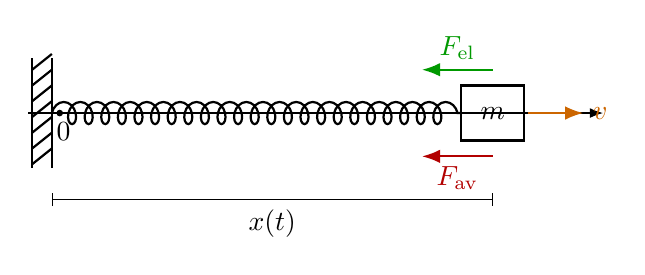
\begin{tikzpicture}[>=Latex,scale=1.0]
  % asse
  \draw[->] (-0.3,0) -- (7.0,0);

  % parete
  \draw[thick] (0, -0.7) -- (0, 0.7);
  \draw[thick] (-0.25, -0.7) -- (-0.25, 0.7);
  \foreach \y in {-0.65,-0.45,...,0.65} {
    \draw[thick] (-0.25,\y) -- (0,\y+0.2);
  }

  % punto di equilibrio
  \fill (0.1,0) circle (1.2pt);
  \node[below] at (0.15,0) {$0$};

  % massa
  \draw[thick] (5.2,-0.35) rectangle (6.0,0.35);
  \node at (5.6,0) {$m$};

  % molla
  \draw[thick,decorate,decoration={coil,aspect=0.7,segment length=6pt,amplitude=4pt}]
    (0,0) -- (5.2,0);

  % frecce forze
  \draw[->,thick,green!60!black] (5.6,0.55) -- (4.7,0.55);
  \node[green!60!black,above] at (5.15,0.55) {$F_{\mathrm{el}}$};

  \draw[->,thick,red!70!black] (5.6,-0.55) -- (4.7,-0.55);
  \node[red!70!black,below] at (5.15,-0.55) {$F_{\mathrm{av}}$};

  % velocità e spostamento
  \draw[->,thick,orange!80!black] (6.05,0.0) -- (6.75,0.0);
  \node[orange!80!black,right] at (6.75,0.0) {$v$};

  \draw[|-|] (0,-1.1) -- (5.6,-1.1);
  \node[below] at (2.8,-1.1) {$x(t)$};
\end{tikzpicture}
\caption{Massa \(m\) collegata a molla e attrito viscoso.}
\end{figure}

\medskip
\textbf{Forze in gioco.}
\begin{itemize}
  \item Forza elastica (legge di Hooke):
  \[
  F_{\mathrm{el}}=-k\,x(t).
  \]
  \item Forza di attrito viscoso:
  \[
  F_{\mathrm{av}}=-\tilde{\gamma}\,v(t)=-\tilde{\gamma}\,\dot x(t).
  \]
\end{itemize}

\textbf{Equazione di Newton.}
Lungo la direzione del moto vale
\[
\sum F = m a \qquad \Longrightarrow \qquad m\,\ddot x(t)=F_{\mathrm{el}}+F_{\mathrm{av}}.
\]
Sostituendo le espressioni delle forze:
\[
m\,\ddot x(t)=-k\,x(t)-\tilde{\gamma}\,\dot x(t).
\]
Dividendo per \(m\):
\[
\ddot x(t)+\frac{\tilde{\gamma}}{m}\,\dot x(t)+\frac{k}{m}\,x(t)=0.
\]

\textbf{Notazioni standard.}
Definiamo
\[
\omega^2=\frac{k}{m},
\qquad
2\gamma=\frac{\tilde{\gamma}}{m}.
\]
Otteniamo infine l’equazione dell’oscillatore armonico smorzato:
\[
\ddot x(t)+2\gamma\,\dot x(t)+\omega^2 x(t)=0.
\]


Nel \textbf{caso (i)} assumiamo
\[
\gamma^2>\omega^2,
\]
quindi le radici dell'equazione caratteristica saranno \emph{reali e distinte}.
\medskip

\inizioapprof

\textbf{Spazio delle soluzioni (campo scalare).}

L'operatore differenziale
\[
L[x]=\ddot x+2\gamma \dot x+\omega^2 x
\]
è lineare. Di conseguenza, l'insieme delle soluzioni reali
\[
\mathcal S_{\mathbb R}
=
\{x:I\to\mathbb R \mid x\in C^2,\ L[x]=0\}
\]
è uno spazio vettoriale su \(\mathbb R\). Inoltre, per teoria standard delle ODE,
\[
\dim_{\mathbb R}(\mathcal S_{\mathbb R})=2:
\]
basta trovare due soluzioni reali linearmente indipendenti per descrivere tutte le soluzioni.

\fineapprof

\medskip

Poiché l'equazione è lineare omogenea a coefficienti costanti, proviamo una soluzione del tipo
\[
x(t)=e^{\lambda t},
\]
con \(\lambda\in\mathbb{C}\). Sostituendo:
\[
\dot x(t)=\lambda e^{\lambda t},
\qquad
\ddot x(t)=\lambda^2 e^{\lambda t}.
\]
Allora
\[
\lambda^2 e^{\lambda t}+2\gamma \lambda e^{\lambda t}+\omega^2 e^{\lambda t}=0.
\]
Poiché \(e^{\lambda t}\neq 0\) per ogni \(t\), otteniamo l'equazione caratteristica
\[
\lambda^2+2\gamma\lambda+\omega^2=0.
\]
Le radici sono
\[
\lambda_{\pm}=-\gamma\pm\sqrt{\gamma^2-\omega^2}.
\]
Nel caso (a) \(\gamma^2-\omega^2>0\), quindi \(\lambda_+\neq \lambda_-\) e \(\lambda_\pm\in\mathbb{R}\).

\medskip
\textbf{Soluzioni fondamentali e combinazione lineare.}
Le funzioni
\[
x_+(t)=e^{\lambda_+ t},
\qquad
x_-(t)=e^{\lambda_- t}
\]
sono due soluzioni reali dell'equazione. Essendo \(\lambda_+\neq\lambda_-\), esse sono linearmente indipendenti su \(\mathbb{R}\).
Per linearità, ogni combinazione lineare reale è ancora soluzione; dunque la soluzione reale generale è
\[
x(t)=A e^{\lambda_+ t}+B e^{\lambda_- t},
\qquad A,B\in\mathbb{R}.
\]

\medskip
\textbf{Nota su esistenza e unicità (dati iniziali reali).}
Assegnati \(x(0)=x_0\in\mathbb{R}\) e \(\dot x(0)=v_0\in\mathbb{R}\), il teorema di Cauchy garantisce esistenza e unicità di una soluzione reale.
In questo caso, la scelta di \(A,B\in\mathbb{R}\) permette di soddisfare univocamente le condizioni iniziali.

\medskip
\textbf{Comportamento asintotico.}
Poiché
\[
\lambda_-=-\gamma-\sqrt{\gamma^2-\omega^2}<0,
\qquad
\lambda_+=-\gamma+\sqrt{\gamma^2-\omega^2}<0
\]
(essendo \(\sqrt{\gamma^2-\omega^2}<\gamma\)), entrambi i termini decadono esponenzialmente e quindi
\[
x(t)\to 0 \qquad \text{per } t\to+\infty.
\]
% Richiede: \usepackage{pgfplots} \pgfplotsset{compat=1.18}

\begin{center}
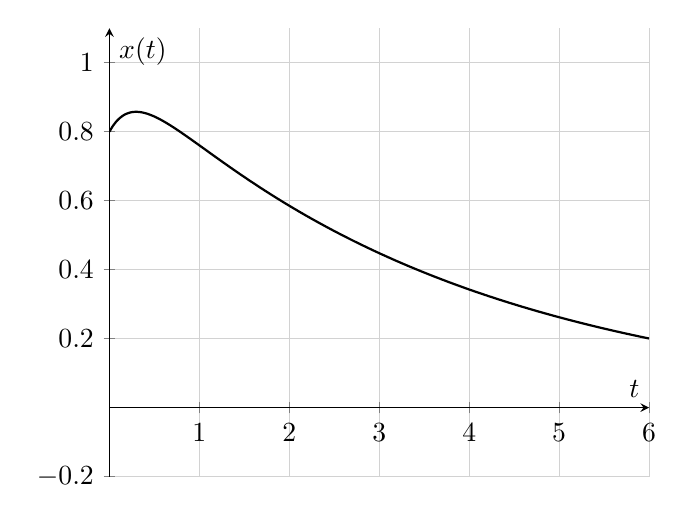
\begin{tikzpicture}
\begin{axis}[
  xlabel={$t$},
  ylabel={$x(t)$},
  axis lines=middle,
  xmin=0, xmax=6,
  ymin=-0.2, ymax=1.1,
  samples=300,
  domain=0:6,
  grid=both,
  grid style={line width=.1pt, draw=gray!25},
  major grid style={line width=.2pt, draw=gray!35},
]
% Caso (a) sovrasmorzato: gamma=2, omega=1 -> lambda_+=-2+sqrt(3), lambda_-=-2-sqrt(3)
% Esempio di soluzione: A=1, B=-0.2 (decadimento senza oscillazioni)
\addplot[thick] {1*exp((-2+sqrt(3))*x) - 0.2*exp((-2-sqrt(3))*x)};
\end{axis}
\end{tikzpicture}
\end{center}
% Richiede: \usepackage{tikz} \usepackage{pgfplots} \pgfplotsset{compat=1.18}


\textbf{Caso (ii): \(\gamma=0\) (oscillatore armonico non smorzato)}

Se \(\gamma=0\), l'equazione diventa
\[
\ddot x+\omega^2 x=0.
\]
Proviamo ancora \(x(t)=e^{\lambda t}\). Sostituendo:
\[
\lambda^2 e^{\lambda t}+\omega^2 e^{\lambda t}=0
\quad\Rightarrow\quad
\lambda^2+\omega^2=0
\quad\Rightarrow\quad
\lambda=\pm i\omega.
\]
Quindi due soluzioni (complesse) sono \(e^{i\omega t}\) ed \(e^{-i\omega t}\), e la soluzione generale (in \(\mathbb{C}\)) è
\[
x(t)=A e^{i\omega t}+B e^{-i\omega t}.
\]

Scriviamo \(A=A_r+iA_i\) e \(B=A_r-iA_i\) (così \(B=\overline{A}\) e \(x(t)\) risulta reale). Allora
\[
x(t)=(A_r+iA_i)e^{i\omega t}+(A_r-iA_i)e^{-i\omega t}.
\]
Usando la formula di Eulero
\[
e^{i\omega t}=\cos(\omega t)+i\sin(\omega t),
\qquad
e^{-i\omega t}=\cos(\omega t)-i\sin(\omega t),
\]
si ottiene
\[
x(t)=(A_r+iA_i)(\cos\omega t+i\sin\omega t)+(A_r-iA_i)(\cos\omega t-i\sin\omega t).
\]
Sviluppando e raccogliendo:
\[
x(t)=2A_r\cos(\omega t)-2A_i\sin(\omega t).
\]
Questa forma si può riscrivere come
\[
x(t)=C\cos(\omega t+\varphi),
\]
dove \(C\) è l'ampiezza e \(\varphi\) la fase (da determinare con le condizioni iniziali), mentre \(\omega\) è un parametro del sistema. Infatti possiamo scrivere
\[
x(t)=2A_r\cos(\omega t)-2A_i\sin(\omega t)
=\sqrt{4A_r^{\,2}+4A_i^{\,2}}
\left(
\frac{A_r}{\sqrt{A_r^{\,2}+A_i^{\,2}}}\cos(\omega t)
-\frac{A_i}{\sqrt{A_r^{\,2}+A_i^{\,2}}}\sin(\omega t)
\right)=
\]
\[
= C\cos(\omega t+\varphi)
\]

\[
\Rightarrow\
\cos\varphi=\frac{A_r}{\sqrt{A_r^{\,2}+A_i^{\,2}}},
\qquad
\sin\varphi=\frac{A_i}{\sqrt{A_r^{\,2}+A_i^{\,2}}},
\qquad
C=\sqrt{4A_r^{\,2}+4A_i^{\,2}}.
\]

\[
\sin\varphi,\ \cos\varphi,\ C\ \text{risultano ben definite perché}
\]

\[
Im\!\left(\frac{A_r}{\sqrt{A_r^{\,2}+A_i^{\,2}}}\right)=[-1,1],
\qquad
Im\!\left(\frac{A_i}{\sqrt{A_r^{\,2}+A_i^{\,2}}}\right)=[-1,1],
\]

\[
Im\!\left(\sqrt{4A_r^{\,2}+4A_i^{\,2}}\right)=[0,+\infty).
\]

Derivando:
\[
\dot x(t)=-C\omega \sin(\omega t+\varphi).
\]
In particolare, imponendo \(x(0)=x_0\) e \(\dot x(0)=v_0\),
\[
x_0=C\cos\varphi,
\qquad
v_0=-C\omega\sin\varphi.
\]
Quindi
\[
\frac{v_0}{x_0}=-\omega\tan\varphi
\quad\Rightarrow\quad
\varphi=\arctan\!\left(-\frac{v_0}{\omega x_0}\right),
\qquad
C=\frac{x_0}{\cos\varphi}.
\]

\begin{center}
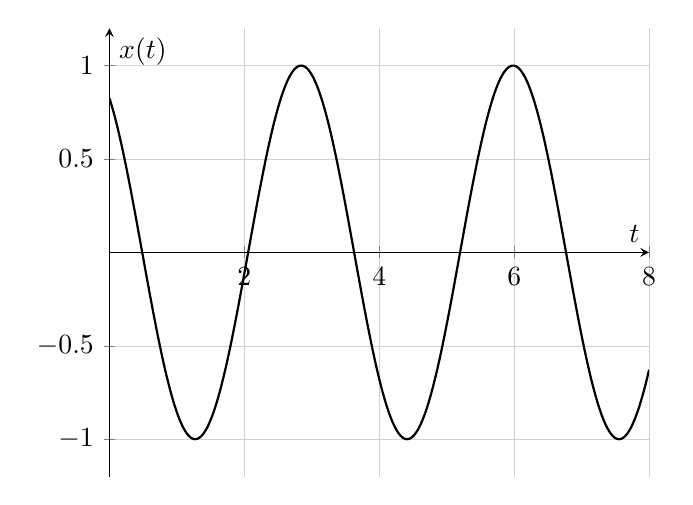
\begin{tikzpicture}
\begin{axis}[
  xlabel={$t$},
  ylabel={$x(t)$},
  axis lines=middle,
  xmin=0, xmax=8,
  ymin=-1.2, ymax=1.2,
  samples=400,
  domain=0:8,
  grid=both,
  grid style={line width=.1pt, draw=gray!25},
  major grid style={line width=.2pt, draw=gray!35},
]
% Esempio: C=1, omega=2, phi=0.6
\addplot[thick] {cos(deg(2*x + 0.6))};
\end{axis}
\end{tikzpicture}
\end{center}


% Richiede: \usepackage{tikz} \usepackage{pgfplots} \pgfplotsset{compat=1.18}


\textbf{Caso (iii): \(\gamma<\omega\) (sottosmorzato)}

Consideriamo
\[
\ddot x(t)+2\gamma\,\dot x(t)+\omega^2 x(t)=0,
\qquad \gamma,\omega>0,
\qquad \gamma<\omega.
\]
Cerchiamo una soluzione del tipo \(x(t)=e^{\lambda t}\). Sostituendo:
\[
\dot x=\lambda e^{\lambda t},\qquad \ddot x=\lambda^2 e^{\lambda t},
\]
si ottiene
\[
\lambda^2 e^{\lambda t}+2\gamma\lambda e^{\lambda t}+\omega^2 e^{\lambda t}=0.
\]
Poiché \(e^{\lambda t}\neq 0\), segue l'equazione caratteristica
\[
\lambda^2+2\gamma\lambda+\omega^2=0.
\]
Le radici sono
\[
\lambda_{\pm}=-\gamma\pm\sqrt{\gamma^2-\omega^2}.
\]
Nel caso \(\gamma<\omega\) vale \(\gamma^2-\omega^2<0\), dunque
\[
\sqrt{\gamma^2-\omega^2}=i\sqrt{\omega^2-\gamma^2}.
\]
Ponendo
\[
\Omega=\sqrt{\omega^2-\gamma^2}>0,
\]
si ottiene
\[
\lambda_{\pm}=-\gamma\pm i\Omega\in\mathbb{C}.
\]

\medskip
\textbf{Soluzione generale (forma complessa).}
Due soluzioni sono \(e^{\lambda_+ t}\) ed \(e^{\lambda_- t}\), quindi
\[
x(t)=A e^{(-\gamma+i\Omega)t}+B e^{(-\gamma-i\Omega)t}.
\]
Raccogliendo \(e^{-\gamma t}\):
\[
x(t)=e^{-\gamma t}\Bigl(A e^{i\Omega t}+B e^{-i\Omega t}\Bigr).
\]

\medskip
\textbf{Passaggio alla forma reale.}
Usiamo le formule di Eulero
\[
e^{i\Omega t}=\cos(\Omega t)+i\sin(\Omega t),\qquad
e^{-i\Omega t}=\cos(\Omega t)-i\sin(\Omega t).
\]
Scegliendo coefficienti tali da ottenere una soluzione reale (equivalentemente, prendendo \(B=\overline{A}\)), l'espressione tra parentesi diventa una combinazione reale di \(\cos(\Omega t)\) e \(\sin(\Omega t)\). Quindi esistono \(C_1,C_2\in\mathbb{R}\) tali che
\[
x(t)=e^{-\gamma t}\Bigl(C_1\cos(\Omega t)+C_2\sin(\Omega t)\Bigr).
\]
Questa forma si riscrive in ampiezza-fase: esistono \(C\ge 0\) e \(\varphi\in\mathbb{R}\) tali che
\[
C_1=C\cos\varphi,\qquad C_2=-C\sin\varphi,
\]
e dunque
\[
x(t)=C e^{-\gamma t}\cos(\Omega t+\varphi).
\]
Questa è un'oscillazione armonica a pulsazione \(\Omega\) con ampiezza modulata dall'inviluppo esponenziale \(e^{-\gamma t}\).

\begin{center}
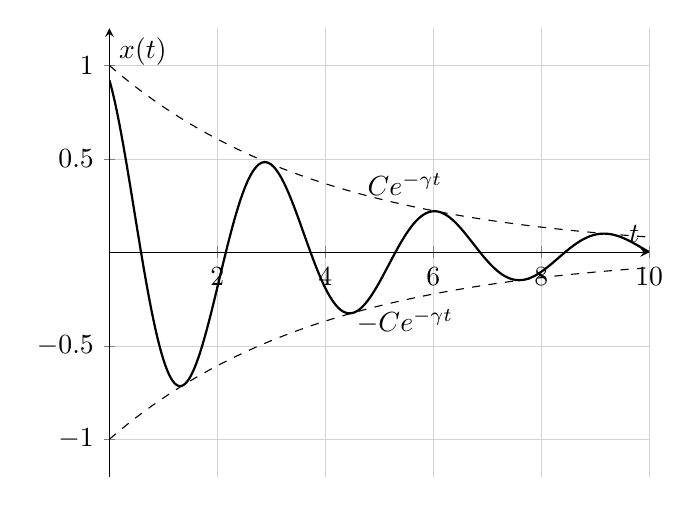
\begin{tikzpicture}
\begin{axis}[
  xlabel={$t$},
  ylabel={$x(t)$},
  axis lines=middle,
  xmin=0, xmax=10,
  ymin=-1.2, ymax=1.2,
  samples=600,
  domain=0:10,
  grid=both,
  grid style={line width=.1pt, draw=gray!25},
  major grid style={line width=.2pt, draw=gray!35},
]
% Esempio numerico: C=1, gamma=0.25, Omega=2, phi=0.4
\addplot[thick] {exp(-0.25*x)*cos(deg(2*x+0.4))};
\addplot[dashed] {exp(-0.25*x)}
  node[pos=0.55, above] {$Ce^{-\gamma t}$};

\addplot[dashed] {-exp(-0.25*x)}
  node[pos=0.55, below] {$-Ce^{-\gamma t}$};
\end{axis}
\end{tikzpicture}
\end{center}
Possiamo riassumere quanto ottenuto finora:
\begin{itemize}
\item \(\gamma=0\) \(\Rightarrow\) nessun attrito: la molla è un oscillatore armonico.

\item \(\gamma>\omega\) \(\Rightarrow\) attrito forte: nessuna oscillazione (oscillatore armonico fortemente smorzato).

\item \(\gamma<\omega\) \(\Rightarrow\) oscillatore che viene smorzato nel tempo dall'attrito \(\bigl(\text{ampiezza}(t)=C e^{-\gamma t}\bigr)\).
\end{itemize}

\begin{oss}{}
Data un'equazione differenziale del \(2^\circ\) ordine possiamo scrivere un sistema di 2 equazioni differenziali del primo ordine ad essa equivalente. Impongo \(x_1=x\), \(x_2=\dot x\).

\[
\ddot x=-2\gamma \dot x-\omega^2 x
\iff
\begin{cases}
\dot x_1=\dot x=x_2,\\
\dot x_2=-2\gamma x_2-\omega^2 x_1.
\end{cases}
\]

\[
\iff\
\frac{d}{dt}
\begin{pmatrix}
x_1\\
x_2
\end{pmatrix}
=
\begin{pmatrix}
0 & 1\\
-\omega^2 & -2\gamma
\end{pmatrix}
\begin{pmatrix}
x_1\\
x_2
\end{pmatrix}.
\]

Notiamo che gli autovalori della matrice
\[
A=
\begin{pmatrix}
0 & 1\\
-\omega^2 & -2\gamma
\end{pmatrix}
\]
sono proprio le radici del polinomio caratteristico di
\[
\ddot x+2\gamma \dot x+\omega^2 x=0,
\qquad\text{ovvero}\qquad
p_A(\lambda)=p(\lambda).
\]
\end{oss}

\textbf{Oscillatore armonico smorzato con forzante periodica}

Consideriamo l’equazione
\[
\ddot{x}+2\gamma \dot{x}+\omega^2 x = F\cos(\Omega t),
\]
dove \(F\) è l’ampiezza della forzante e \(\Omega\) la sua pulsazione.

Poiché l’equazione è lineare, la soluzione generale della non omogenea è somma di una soluzione generale dell’omogenea e di una particolare:
\[
x(t)=x_0(t)+x_p(t),
\]
con
\[
\ddot{x}_0+2\gamma \dot{x}_0+\omega^2 x_0=0,
\qquad
\ddot{x}_p+2\gamma \dot{x}_p+\omega^2 x_p=F\cos(\Omega t).
\]

\medskip
\textbf{Caso \(\gamma=0\).}
L’equazione diventa
\[
\ddot{x}+\omega^2 x = F\cos(\Omega t).
\]
Cerchiamo una particolare del tipo \(x_p(t)=D\cos(\Omega t)\). Allora
\[
\ddot{x}_p(t)=-D\Omega^2\cos(\Omega t),
\]
e sostituendo:
\[
-D\Omega^2\cos(\Omega t)+\omega^2 D\cos(\Omega t)=F\cos(\Omega t)
\quad\Rightarrow\quad
D(\omega^2-\Omega^2)=F.
\]
Quindi, se \(\Omega\neq\omega\),
\[
D=\frac{F}{\omega^2-\Omega^2},
\qquad
x_p(t)=\frac{F}{\omega^2-\Omega^2}\cos(\Omega t).
\]
La soluzione generale è allora
\[
x(t)=C\cos(\omega t+\varphi)+\frac{F}{\omega^2-\Omega^2}\cos(\Omega t),
\]
dove \(C\) e \(\varphi\) si determinano dalle condizioni iniziali. In particolare, imponendo
\(x(0)=x_0\) e \(\dot{x}(0)=v_0\),
\[
x_0=C\cos\varphi+\frac{F}{\omega^2-\Omega^2}\cos(0),
\]
\[
v_0=-\omega C\sin\varphi-\frac{F}{\omega^2-\Omega^2}\,\Omega\sin(0).
\]

\medskip
\textbf{Caso \(\gamma\neq 0\).}
Proviamo una particolare del tipo
\[
x_p(t)=D\cos(\Omega t+\beta).
\]
Allora
\[
\dot{x}_p(t)=-D\Omega\sin(\Omega t+\beta),
\qquad
\ddot{x}_p(t)=-D\Omega^2\cos(\Omega t+\beta).
\]
Sostituendo nell’equazione:
\[
(\omega^2-\Omega^2)D\cos(\Omega t+\beta)-2\gamma\Omega D\sin(\Omega t+\beta)=F\cos(\Omega t).
\]
Usando
\[
\cos(\Omega t+\beta)=\cos(\Omega t)\cos\beta-\sin(\Omega t)\sin\beta,
\]
\[
\sin(\Omega t+\beta)=\sin(\Omega t)\cos\beta+\cos(\Omega t)\sin\beta,
\]
si ottiene
\[
\cos(\Omega t)\,D\bigl[(\omega^2-\Omega^2)\cos\beta-2\gamma\Omega\sin\beta\bigr]
+\sin(\Omega t)\,D\bigl[-(\omega^2-\Omega^2)\sin\beta-2\gamma\Omega\cos\beta\bigr] =
\]
\[
=F\cos(\Omega t)+0\cdot\sin(\Omega t).
\]
Eguagliando i coefficienti di \(\cos(\Omega t)\) e \(\sin(\Omega t)\) si ottiene il sistema
\[
\begin{cases}
D\bigl[(\omega^2-\Omega^2)\cos\beta-2\gamma\Omega\sin\beta\bigr]=F,\\[4pt]
D\bigl[(\omega^2-\Omega^2)\sin\beta+2\gamma\Omega\cos\beta\bigr]=0.
\end{cases}
\]
Dalla seconda equazione:
\[
(\omega^2-\Omega^2)\sin\beta+2\gamma\Omega\cos\beta=0
\quad\Rightarrow\quad
\tan\beta=-\dfrac{2\gamma\Omega}{\omega^2-\Omega^2}
=\dfrac{2\gamma\Omega}{\Omega^2-\omega^2}.
\]
Inoltre, elevando al quadrato e sommando le due equazioni del sistema si ricava
\[
D^2\bigl[(\omega^2-\Omega^2)^2+(2\gamma\Omega)^2\bigr]=F^2
\quad\Rightarrow\quad
D=\frac{F}{\sqrt{(\omega^2-\Omega^2)^2+(2\gamma\Omega)^2}}.
\]

\medskip
\textbf{Soluzione generale (caso \(\gamma<\omega\)).}
Se \(\gamma<\omega\), la soluzione dell’omogenea è
\[
x_0(t)=C\,e^{-\gamma t}\cos\!\bigl(\sqrt{\omega^2-\gamma^2}\,t+\varphi\bigr),
\]
e quindi la soluzione generale della forzata è
\[
x(t)=C\,e^{-\gamma t}\cos\!\bigl(\sqrt{\omega^2-\gamma^2}\,t+\varphi\bigr)
+ D\cos(\Omega t+\beta),
\]
con
\[
D=\frac{F}{\sqrt{(\omega^2-\Omega^2)^2+(2\gamma\Omega)^2}},
\qquad
\tan\beta=\frac{2\gamma\Omega}{\Omega^2-\omega^2}.
\]

\begin{oss}{}
Nel caso \(\gamma>0\) il termine transiente \(x_0(t)\) decade esponenzialmente, quindi
\[
\lim_{t\to+\infty} x(t) = \text{(componente forzata)} \quad\Rightarrow\quad
x(t)\sim D\cos(\Omega t+\beta)\ \ \text{per } t\to+\infty.
\]
In altre parole, il sistema “dimentica” le condizioni iniziali: a regime resta solo l’oscillazione alla frequenza della forzante.
\end{oss}

\chapter{Moti di punti materiali e vincoli.}
\section{Moto di un punto materiale}
\begin{center}
    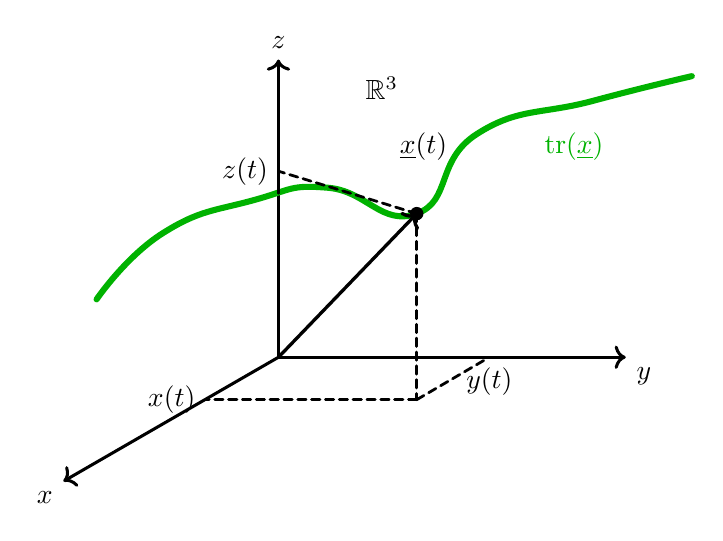
\begin{tikzpicture}[scale=1.05, line cap=round, line join=round]

% --- assi in "prospettiva" (2D) ---
\coordinate (O) at (0,0);
\coordinate (X) at (-2.6,-1.5);
\coordinate (Y) at (4.2,0);
\coordinate (Z) at (0,3.6);

\draw[->,line width=1.1pt] (O) -- (X) node[below left] {$x$};
\draw[->,line width=1.1pt] (O) -- (Y) node[below right] {$y$};
\draw[->,line width=1.1pt] (O) -- (Z) node[above] {$z$};

% --- base per le coordinate in 2D ---
\coordinate (Xhat) at (-0.65,-0.38);
\coordinate (Yhat) at (1,0);
\coordinate (Zhat) at (0,1);

% punto P = a*Xhat + b*Yhat + c*Zhat
\def\xa{1.35}
\def\yb{2.55}
\def\zc{2.25}
\coordinate (P) at ({\xa*(-0.65)+\yb},{\xa*(-0.38)+\zc});

% proiezioni
\coordinate (Px) at ({\xa*(-0.65)},{\xa*(-0.38)});
\coordinate (Py) at (\yb,0);
\coordinate (Pz) at (0,\zc);
\coordinate (Pxy) at ({\xa*(-0.65)+\yb},{\xa*(-0.38)});
\node[black,anchor=west] at (\xa , \yb) {$\underline{x}(t)$};

% --- traiettoria verde (passa ESATTAMENTE per P) ---
\draw[green!70!black,line width=2.2pt]
  plot[smooth,tension=0.85]
  coordinates {(-2.2,0.7) (-1.4,1.5) (-0.3,1.9) (0.6,2.05) (P) (2.4,2.7) (3.8,3.1) (5.0,3.4)};
\node[green!70!black,anchor=west] at (3.1,2.55) { $\operatorname{tr}(\underline{x})$};

% --- vettore posizione ---
\draw[->,line width=1.2pt] (O) -- (P);

% --- punto ---
\fill (P) circle (2.3pt);

% --- proiezioni tratteggiate ---
\draw[densely dashed,line width=1.0pt] (P) -- (Pxy);
\draw[densely dashed,line width=1.0pt] (Pxy) -- (Py) node[below] {$y(t)$};
\draw[densely dashed,line width=1.0pt] (Pxy) -- (Px) node[left] {$x(t)$};
\draw[densely dashed,line width=1.0pt] (P) -- (Pz) node[left] {$z(t)$};
\draw[densely dashed,line width=1.0pt] (Pz) -- (O);

% etichette extra
\node at (1.25,3.25) {$\mathbb{R}^3$};


\end{tikzpicture}
\end{center}
Possiamo modellare il moto di un punto materiale tramite una legge oraria del tipo
\[
\underline{x}(t) = (x(t) , y(t) , z(t))
\]
Matematicamente stiamo descrivendo una curva parametrizzata in $\mathbb{R}^3$ del tipo $\underline{x}:[0 , t_f] \to \mathbb{R}^3$.
\begin{oss}{}
La stessa traccia (traiettoria) può essere percorsa con diverse leggi orarie $\underline{x}(t)$ che matematicamente corrispondono a diverse riparametrizzazioni equivalenti di una curva.
\end{oss}
Possiamo quindi definire la velocità della curva come il vettore tangente alla curva dato da
\[
 \underline{v}(t)= \underline{\dot{x}}(t) =\frac{d\underline{x}}{dt}
=\left(\frac{dx}{dt},\,\frac{dy}{dt},\,\frac{dz}{dt}\right)
\]
e il vettore accelerazione dato da
\[
\frac{d^2\underline{x}}{dt^2}=\underline{a}
=\frac{d\underline{v}}{dt}
=(a_x,a_y,a_z).
\]

\begin{center}
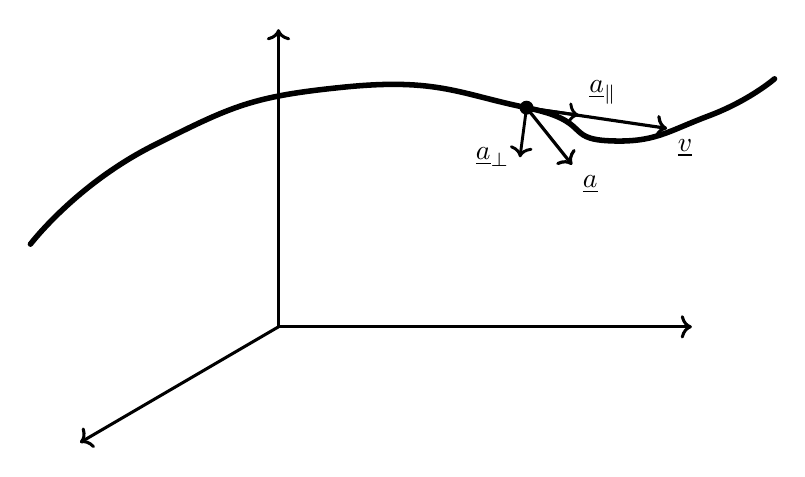
\begin{tikzpicture}[scale=1.05, line cap=round, line join=round]

% --- assi in "prospettiva" (2D) ---
\coordinate (O) at (0,0);
\draw[->,line width=1.1pt] (O) -- (-2.4,-1.4);
\draw[->,line width=1.1pt] (O) -- (5.0,0);
\draw[->,line width=1.1pt] (O) -- (0,3.6);

% --- punto sulla curva ---
\coordinate (P) at (3.0,2.65);
\fill (P) circle (2.4pt);

% --- curva (passa per P) ---
\draw[line width=2.0pt]
  plot[smooth,tension=0.9]
  coordinates {(-3.0,1.0) (-1.5,2.2) (0.8,2.9) (P) (4.0,2.25) (5.2,2.55) (6.0,3.0)};

% --- vettore velocità (tangente) ---
\draw[->,line width=1.15pt] (P) -- ++(1.7,-0.25)
  node[below right] {$\underline{v}$};

% --- accelerazione totale (ancora più piccola) ---
\coordinate (Aend) at ($(P)+(0.55,-0.69)$); % più corta
\draw[->,line width=1.15pt] (P) -- (Aend)
  node[below right] {$\underline{a}$};

% --- componenti: a parallela e a perpendicolare (somma = a) ---
\coordinate (Apar)  at ($(P)+(0.63,-0.09)$);
\coordinate (Aperp) at ($(P)+(-0.08,-0.60)$);

\draw[->,line width=1.05pt] (P) -- (Apar)
  node[above right] {$\underline{a}_{\parallel}$};

\draw[->,line width=1.05pt] (P) -- (Aperp)
  node[left] {$\underline{a}_{\perp}$};

\end{tikzpicture}
\end{center}

Possiamo descrivere un moto in coordinate diverse dalle coordinate cartesiane.\\
Se il moto è nel piano ($z=0$) allora una scelta di coordinate può essere quella delle coordinate polari.
\begin{center}
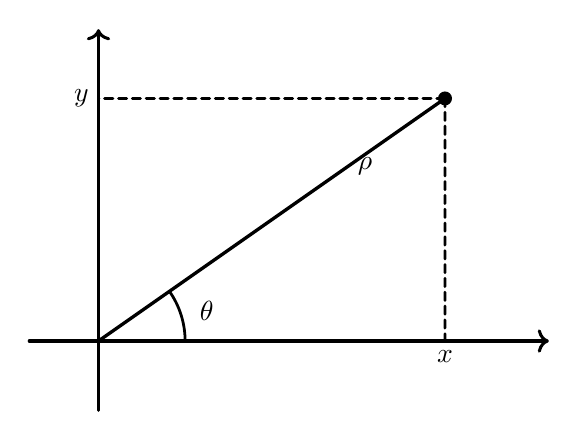
\begin{tikzpicture}[scale=1.1, line cap=round, line join=round]

% assi
\draw[->,line width=1.1pt] (-0.8,0) -- (5.2,0);
\draw[->,line width=1.1pt] (0,-0.8) -- (0,3.6);

% punto finale
\coordinate (P) at (4,2.8);
\fill (P) circle (2.3pt);

% vettore r
\draw[line width=1.2pt] (0,0) -- (P);
\node[ right] at ($(0,0)!0.72!(P)$) {$\rho$};

% proiezioni tratteggiate
\draw[densely dashed,line width=1.0pt] (P) -- (4,0);
\draw[densely dashed,line width=1.0pt] (P) -- (0,2.8);

% etichette assi vicino alle proiezioni
\node[below] at (4,0) {$x$};
\node[left]  at (0,2.8) {$y$};

% angolo theta
\draw[line width=1.0pt] (1,0) arc[start angle=0,end angle=35,radius=1];
\node at (1.25,0.35) {$\theta$};

\end{tikzpicture}
\end{center}

Le coordinate polari sono date da
\[
(\rho(x(t) , y(t)) , \theta(x(t) , y(t))) = (\sqrt{x^2 +y^2} , \operatorname{arctg}(y/x))
\]
o equivalentemente da
\[
\underline{x}(t) = (x(\theta(t) , \rho(t)) ,y(\theta(t) , \rho(t))) = (\rho \cos\theta  , \rho\sin\theta)
\]
Possiamo anche riscrivere $\underline{v}(t)$ attraverso le coordinate polari.
\[
v_x=\frac{dx}{dt}
=\frac{d}{dt}\bigl(\rho\cos\theta\bigr)
=\frac{d\rho}{dt}\cos\theta-\rho\sin\theta\,\frac{d\theta}{dt}
=\dot{\rho}\cos\theta-\rho\sin\theta\,\dot{\theta}.
\]

\[
v_y=\frac{dy}{dt}
=\frac{d}{dt}\bigl(\rho\sin\theta\bigr)
=\dot{\rho}\sin\theta+\rho\dot{\theta}\cos\theta.
\]

\[
\underline{v}=(v_x,v_y)
=
\dot{\rho}
\begin{pmatrix}
\cos\theta\\
\sin\theta
\end{pmatrix}
+
\rho\dot{\theta}
\begin{pmatrix}
-\sin\theta\\
\cos\theta
\end{pmatrix} = \dot{\rho} \cdot \underline{e_\rho} + \rho \dot{\theta} \cdot \underline{e_\theta} , \quad \underline{e_\rho}\cdot \underline{e_\theta}=0
\]

\begin{center}
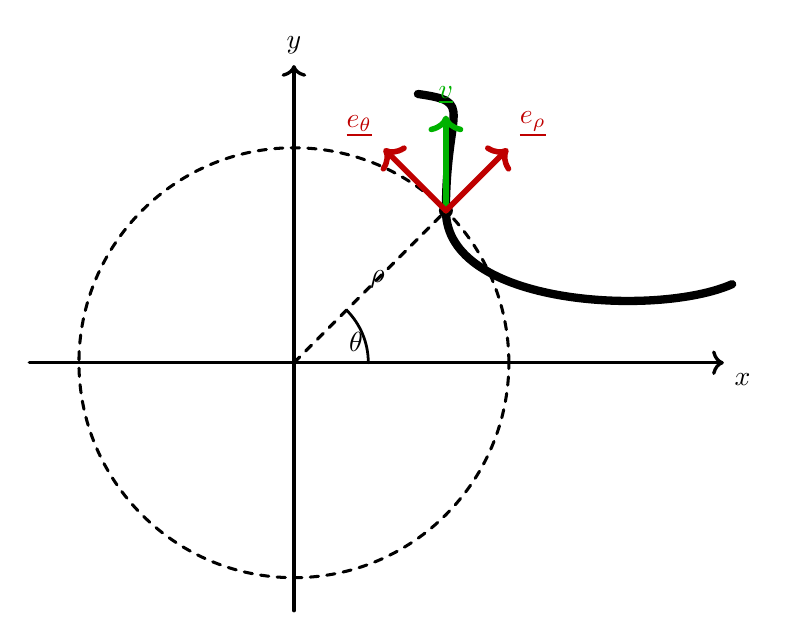
\begin{tikzpicture}[scale=1.05, line cap=round, line join=round]

% assi
\draw[->,line width=1.2pt] (-3.2,0) -- (5.2,0) node[below right] {$x$};
\draw[->,line width=1.2pt] (0,-3.0) -- (0,3.6) node[above] {$y$};

% circonferenza tratteggiata
\pgfmathsetmacro{\R}{2.6}
\draw[dashed, line width=1.1pt] (0,0) circle (\R);

% punto P sulla circonferenza a 45°
\pgfmathsetmacro{\Px}{\R/sqrt(2)}
\pgfmathsetmacro{\Py}{\R/sqrt(2)}
\coordinate (P) at (\Px,\Py);

% raggio tratteggiato
\draw[dashed, line width=1.1pt] (0,0) -- (P);

% punto
\fill (P) circle (2.4pt);

% --- curva nera: due Bézier che si incontrano in P con tangente verticale ---
% scegli due punti finali della curva (a sinistra-alto e a destra-basso)
\coordinate (A) at (1.5,3.25);
\coordinate (B) at (5.3,0.95);

% controlli: quelli vicini a P sono verticali (stesso x = Px) => tangente verticale in P
\coordinate (c1) at (2.2,3.15);            % controllo vicino ad A
\coordinate (c2) at (\Px,\Py+1.25);        % controllo sopra P (verticale)
\coordinate (c3) at (\Px,\Py-1.15);        % controllo sotto P (verticale)
\coordinate (c4) at (4.4,0.55);            % controllo vicino a B

\draw[line width=3.0pt]
  (A) .. controls (c1) and (c2) .. (P)
      .. controls (c3) and (c4) .. (B);

% --- vettori in P ---
% v: tangente alla curva in P (verticale)
\draw[->,green!70!black,line width=2.0pt] (P) -- ++(0,1.15)
  node[above] {$\underline{v}$};

% t: tangente alla circonferenza in P (direzione (-1,1))
\draw[->,red!75!black,line width=2.0pt] (P) -- ++(-0.75,0.75)
  node[above left] {$\underline{e_\theta}$};

% m: radiale (perpendicolare alla circonferenza) in P (direzione (1,1))
\draw[->,red!75!black,line width=2.0pt] (P) -- ++(0.75,0.75)
  node[above right] {$\underline{e_\rho}$};
% angolo \theta (archetto all'origine tra asse x e raggio OP)
\draw[line width=1.0pt] (0.9,0) arc[start angle=0,end angle=45,radius=0.9];
\node at (0.75,0.25) {$\theta$};

% lunghezza \rho sul raggio (etichetta lungo il segmento OP)
\node at ($(0,0)!0.55!(P)$) {$\rho$};
\end{tikzpicture}
\end{center}
\begin{oss}{}
    Il versore $\underline{e_\theta}$ non è tangente alla curva ma alla circonferenza centrata nell'origine di raggio $\rho$ nel punto $\underline{x}(t)$. Di conseguenza non è tangente alla velocità.
\end{oss}
Ricaviamo infine il vettore accelerazione $\underline{a}(t)$ in coordinate polari.
\[
a_x=\frac{dv_x}{dt}
=\frac{d}{dt}\bigl(\dot{\rho}\cos\theta-\rho\,\dot{\theta}\sin\theta\bigr)
=\ddot{\rho}\cos\theta-\dot{\rho}\dot{\theta}\sin\theta-\dot{\rho}\dot{\theta}\sin\theta
-\rho\,\frac{d}{dt}\bigl(\dot{\theta}\sin\theta\bigr)
\]
\[
=\ddot{\rho}\cos\theta-2\dot{\rho}\dot{\theta}\sin\theta
-\rho\Bigl(\ddot{\theta}\sin\theta+(\dot{\theta})^2\cos\theta\Bigr)
\]
\[
=\ddot{\rho}\cos\theta-2\dot{\rho}\dot{\theta}\sin\theta-\rho\,\ddot{\theta}\sin\theta-\rho(\dot{\theta})^2\cos\theta
\]
\[
=\bigl(\ddot{\rho}-\rho(\dot{\theta})^2\bigr)\cos\theta-\bigl(2\dot{\rho}\dot{\theta}+\rho\ddot{\theta}\bigr)\sin\theta.
\]

\[
a_y=\frac{d}{dt}v_y
=\frac{d}{dt}\bigl(\dot{\rho}\sin\theta+\rho\,\dot{\theta}\cos\theta\bigr)
=\ddot{\rho}\sin\theta+\dot{\rho}\dot{\theta}\cos\theta+\dot{\rho}\dot{\theta}\cos\theta
+\rho\,\frac{d}{dt}\bigl(\dot{\theta}\cos\theta\bigr)
\]
\[
=\ddot{\rho}\sin\theta+2\dot{\rho}\dot{\theta}\cos\theta
+\rho\Bigl(\ddot{\theta}\cos\theta-(\dot{\theta})^2\sin\theta\Bigr)
\]
\[
=\ddot{\rho}\sin\theta+2\dot{\rho}\dot{\theta}\cos\theta+\rho\,\ddot{\theta}\cos\theta-\rho(\dot{\theta})^2\sin\theta
\]
\[
=\bigl(\ddot{\rho}-\rho(\dot{\theta})^2\bigr)\sin\theta+\bigl(\rho\ddot{\theta}+2\dot{\rho}\dot{\theta}\bigr)\cos\theta.
\]

\[
\Rightarrow\quad
\underline{a}=(a_x,a_y)
=\bigl(\ddot{\rho}-\rho\dot{\theta}^{\,2}\bigr)\,
\underbrace{\begin{pmatrix}\cos\theta\\ \sin\theta\end{pmatrix}}_{\underline{e}_{\rho}}
+\bigl(\rho\ddot{\theta}+2\dot{\rho}\dot{\theta}\bigr)\,
\underbrace{\begin{pmatrix}-\sin\theta\\ \cos\theta\end{pmatrix}}_{\underline{e}_{\theta}}.
\]

Per un generico moto (e quindi per una generica traiettoria) le coordinate polari non hanno un reale vantaggio, anzi complicano di parecchio le cose. Possono però essere utili per descrivere specifici moti ad esempio il moto circolare di raggio costante $R$.

\begin{itemize}
\item Con le coordinate cartesiane devo avere 2 informazioni per definire
$\underline{x}(t)$, $\underline{v}(t)$, $\underline{a}(t)$.

\item Se uso le coordinate polari $\rho=R$ definisco il moto fornendo solamente un'informazione ovvero $\theta(t)$.
\end{itemize}
\begin{center}
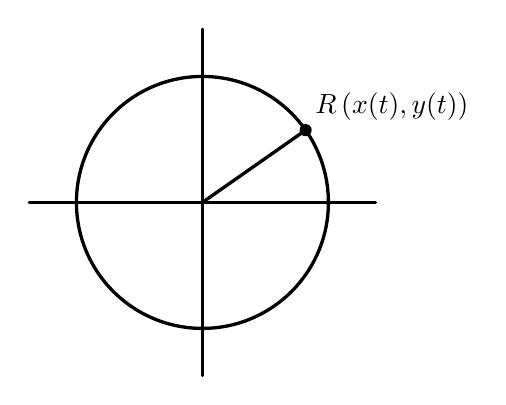
\begin{tikzpicture}[scale=1.0, line cap=round, line join=round]
  \def\R{1.6}
  \def\ang{35}

  % assi
  \draw[line width=1.1pt] (-2.2,0) -- (2.2,0);
  \draw[line width=1.1pt] (0,-2.2) -- (0,2.2);

  % cerchio
  \draw[line width=1.2pt] (0,0) circle (\R);

  % punto e raggio
  \coordinate (P) at ({\R*cos(\ang)},{\R*sin(\ang)});
  \draw[line width=1.2pt] (0,0) -- (P);
  \fill (P) circle (2.2pt);

  % etichetta R(x(t),y(t))
  \node[above right] at (P) {$R\,(x(t),y(t))$};
\end{tikzpicture}
\end{center}
La velocità infatti diventa
\[
\underline{v}=\rho\,\dot{\theta}
\begin{pmatrix}
-\sin\theta\\
\cos\theta
\end{pmatrix}
=R\dot{\theta}\,\underline{t}.
\]
\begin{center}
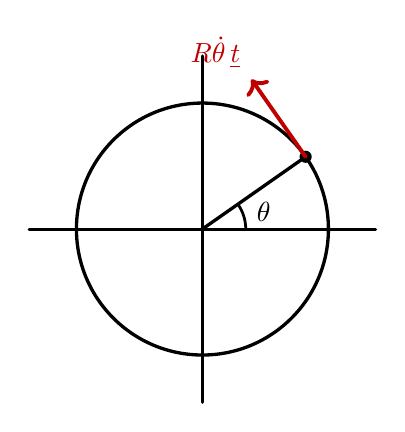
\begin{tikzpicture}[scale=1.0, line cap=round, line join=round]
  \def\R{1.6}
  \def\ang{35}

  % assi
  \draw[line width=1.1pt] (-2.2,0) -- (2.2,0);
  \draw[line width=1.1pt] (0,-2.2) -- (0,2.2);

  % cerchio
  \draw[line width=1.2pt] (0,0) circle (\R);

  % punto e raggio
  \coordinate (P) at ({\R*cos(\ang)},{\R*sin(\ang)});
  \draw[line width=1.2pt] (0,0) -- (P);
  \fill (P) circle (2.2pt);

  % angolo theta
  \draw[line width=1.0pt] (0.55,0) arc[start angle=0,end angle=\ang,radius=0.55];
  \node at (0.78,0.22) {$\theta$};

  % velocità: R dot(theta) t
  \draw[->,red!75!black,line width=1.4pt]
    (P) -- ++({-1.2*sin(\ang)},{1.2*cos(\ang)})
    node[above left] {$R\dot{\theta}\,\underline{t}$};
\end{tikzpicture}
\end{center}
mentre l'accelerazione diventa
\[
\underline{a}
=-R\dot{\theta}^{\,2}
\begin{pmatrix}
\cos\theta\\
\sin\theta
\end{pmatrix}
+R\ddot{\theta}
\begin{pmatrix}
-\sin\theta\\
\cos\theta
\end{pmatrix}
=
-R\dot{\theta}^{\,2}\,\underline{n}+R\ddot{\theta}\,\underline{t}.
\]

\begin{center}
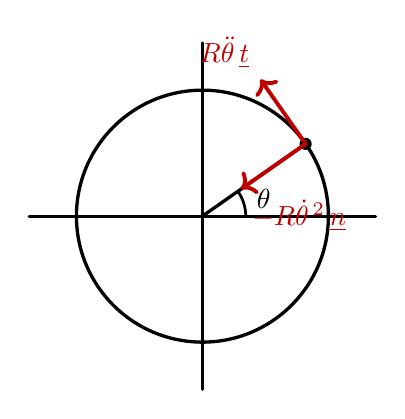
\begin{tikzpicture}[scale=1.0, line cap=round, line join=round]
  \def\R{1.6}
  \def\ang{35}

  % assi
  \draw[line width=1.1pt] (-2.2,0) -- (2.2,0);
  \draw[line width=1.1pt] (0,-2.2) -- (0,2.2);

  % cerchio
  \draw[line width=1.2pt] (0,0) circle (\R);

  % punto e raggio
  \coordinate (P) at ({\R*cos(\ang)},{\R*sin(\ang)});
  \draw[line width=1.2pt] (0,0) -- (P);
  \fill (P) circle (2.2pt);

  % angolo theta
  \draw[line width=1.0pt] (0.55,0) arc[start angle=0,end angle=\ang,radius=0.55];
  \node at (0.78,0.22) {$\theta$};

  % componente tangenziale: R ddot(theta) t
  \draw[->,red!75!black,line width=1.4pt]
    (P) -- ++({-1.0*sin(\ang)},{1.0*cos(\ang)})
    node[above left] {$R\ddot{\theta}\,\underline{t}$};

  % componente normale: -R dot(theta)^2 m (verso il centro)
  \draw[->,red!75!black,line width=1.4pt]
    (P) -- ++({-1.0*cos(\ang)},{-1.0*sin(\ang)})
    node[below right] {$-R\dot{\theta}^{\,2}\,\underline{n}$};
\end{tikzpicture}
\end{center}
\begin{oss}{}
 $\ddot{\theta}(t)$ potrebbe essere negativo e quindi $R\ddot{\theta}\,\underline{t}$ potrebbe avere direzione $-\underline{t}$.
\end{oss}

\begin{oss}{}
    In questo caso i versori $\underline{e_\theta}, \underline{e_\rho}$ corrispondono (a meno del verso) con i versori $\underline{n} , \underline{t}$ normale e tangente alla curva.
\end{oss}

\section{Introduzione ai vincoli e loro classificazione}
Nel paragrafo precedente abbiamo introdotto la descrizione cinematica di un punto materiale. Consideriamo ora un insieme di $n$ punti materiali detto sistema di punti materiali. Ogni punto del sistema è descritto da una legge oraria
\[
\underline{x_i} (t) = (x_i(t) , y_i(t) , z_i(t)) \quad \forall i = 1 \ldots , n
\]
In generale, un sistema di $n$ punti  materiali non è completamente libero: i punti sono spesso soggetti a restrizioni geometriche o cinematiche, dette vincoli, che ne limitano i moti ammissibili legando tra loro le coordinate.\\
Queste condizioni e relazioni sul moto vengono dette $\textbf{vincoli}$.
\begin{example}{}
    Consideriamo un punto che si muove di moto piano. La sua traiettoria è descritta da una curva del tipo
    \[
    \underline{x}(t) = (x(t) , y(t) , z(t))
    \]
    e dal vincolo $z = 0$. Per descrivere il moto del punto sono quindi sufficienti 2 informazioni che in questo caso corrispondono a $(x(t) , y(t))$.
\end{example}

\begin{example}{}
    Possiamo rivedere l'esempio del moto circolare nell'ottica dei vincoli. Abbiamo 1 punto che si muove con traiettoria $(x(t) , y(t) , z(t))$ e 2 vincoli ovvero
    \[
    \begin{cases}
        z = 0 \\
        x^2 + y^2 = R^2
    \end{cases}
    \]
    Il sistema può essere descritto da una sola coordinata $\theta(t)$
\end{example}

\begin{example}{}
Consideriamo $2$ punti materiali nello spazio:
\[
\bigl(x_1(t),y_1(t),z_1(t)\bigr), \qquad \bigl(x_2(t),y_2(t),z_2(t)\bigr).
\]
In assenza di vincoli, per descrivere il sistema servono $6$ coordinate (tre per ciascun punto).

Supponiamo ora di imporre il vincolo che la distanza tra i due punti sia fissata e pari a $d$. Il vincolo si scrive come
\[
\bigl(x_1-x_2\bigr)^2+\bigl(y_1-y_2\bigr)^2+\bigl(z_1-z_2\bigr)^2=d^2.
\]
Il sistema può essere descritto da 5 coordinate.
\end{example}

\begin{example}{}
Consideriamo un punto materiale nello spazio:
\[
\bigl(x(t),y(t),z(t)\bigr).
\]
In assenza di vincoli, per descrivere il sistema servono $3$ coordinate.

Supponiamo ora che il punto sia vincolato a muoversi su una superficie sferica di raggio $R$. Il vincolo si scrive come
\[
x^2+y^2+z^2=R^2.
\]
Il sistema può essere descritto da 2 coordinate.
\end{example}

\begin{example}{}
Consideriamo il moto di due punti materiali sul piano con distanza fissata tra di loro:
\[
\bigl(x_1(t),y_1(t),z_1(t)\bigr),\qquad \bigl(x_2(t),y_2(t),z_2(t)\bigr).
\]
I vincoli sono
\[
z_1=0,\qquad z_2=0,\qquad (x_1-x_2)^2+(y_1-y_2)^2=d^2.
\]

Possiamo usare coordinate ``convenienti'': ad esempio scegliere come coordinate indipendenti
\[
(x_1(t),\,y_1(t),\,\theta(t)),
\]
dove $\theta(t)$ è l'angolo che il segmento che unisce i due punti forma con l'asse $x$ e dove $x_1 , y_1$ sono le coordinate nel piano del centro del segmento che li congiunge.

\medskip

\begin{center}
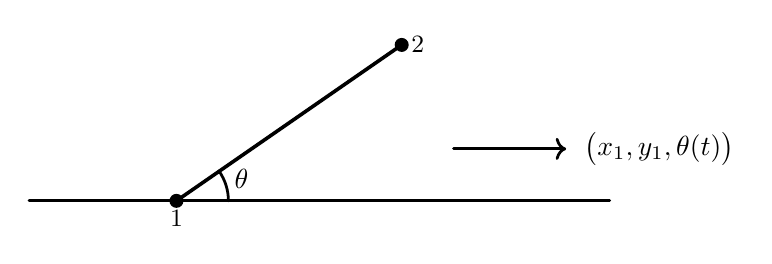
\begin{tikzpicture}[scale=1.1, line cap=round, line join=round]

% asse orizzontale
\draw[line width=1.1pt] (-0.5,0) -- (6.2,0);

% punti 1 e 2
\coordinate (P1) at (1.2,0);
\coordinate (P2) at (3.8,1.8);

\fill (P1) circle (2.3pt) node[below] {\small $1$};
\fill (P2) circle (2.3pt) node[right] {\small $2$};

% segmento tra i punti
\draw[line width=1.3pt] (P1) -- (P2);

% angolo theta in P1
\draw[line width=1.0pt] (1.8,0) arc[start angle=0,end angle=35,radius=0.6];
\node at (1.95,0.25) {$\theta$};

% freccia e testo (x1,y1,theta(t))
\draw[->,line width=1.0pt] (4.4,0.6) -- (5.7,0.6);
\node[anchor=west] at (5.8,0.6) {$\bigl(x_1,y_1,\theta(t)\bigr)$};

\end{tikzpicture}
\end{center}
\end{example}

Dopo aver visto alcuni esempi introduttivi presentiamo una classificazione dei vincoli.
\begin{itemize}
\item \textbf{Monolatero posizionale:}
\[
g(x_1,x_2,\dots,x_m,t)\ge 0.
\]

\item \textbf{Monolatero posizionale indipendente dal tempo:}
\[
g(x_1,x_2,\dots,x_m)\ge 0.
\]

\item \textbf{Bilatero posizionale:}
\[
g(x_1,\dots,x_m,t)=0.
\]

\item \textbf{Bilatero posizionale indipendente dal tempo:}
\[
g(x_1,\dots,x_m)=0.
\]
\end{itemize}

\begin{example}{}
(\textbf{Monolatero posizionale}) Un punto vincolato a rimanere nel semispazio superiore:
\[
z(t)\ge 0.
\]
\end{example}

\begin{example}{}
(\textbf{Bilatero posizionale, dipendente dal tempo}) Un punto vincolato a stare su una circonferenza di raggio $R(t)$, dove $R(t)$ è una legge nota:
\[
g\bigl((x(t),y(t)),t\bigr)=x^2(t)+y^2(t)-R^2(t)=0.
\]
\end{example}

\begin{example}{}
(\textbf{Monolatero posizionale, dipendente dal tempo}) Un punto vincolato a stare all'esterno (o sul bordo) della circonferenza di raggio $R(t)$:
\[
x^2(t)+y^2(t)-R^2(t)\ge 0.
\]
\end{example}

\begin{itemize}
\item \textbf{Vincoli dipendenti dalla velocità non integrabili:}
\[
g(v_1,\dots,v_m)=0.
\]
\end{itemize}

\begin{oss}{}
Esistono vincoli sulla velocità ma \emph{integrabili} che sono in realtà vincoli posizionali.
\end{oss}

\begin{example}{}
Un punto materiale con coordinate $(x,y,z)$ soggetto al vincolo
\[
v_z=0.
\]
Poiché
\[
v_z=\frac{dz}{dt},
\]
segue che
\[
\frac{dz}{dt}=0 \;\Rightarrow\; z=\text{costante},
\]
cioè il moto è piano.
\end{example}

Dato un sistema di punti materiali
\[
\bigl(\underline{x}_1(t),\dots,\underline{x}_m(t)\bigr),
\]
diciamo che il sistema è soggetto a \textbf{vincoli olonomi} se i vincoli sono \emph{posizionali, bilateri e indipendenti}.
Supponiamo che ci siano $s$ vincoli olonomi, espressi da $s$ relazioni indipendenti
\[
g_k\bigl(\underline{x}_1,\dots,\underline{x}_m,t\bigr)=0,
\qquad k=1,\dots,s.
\]

Poiché ciascun punto in $\mathbb{R}^3$ richiede $3$ coordinate, le coordinate cartesiane complessive sono $3m$.
L'imposizione di $s$ vincoli olonomi indipendenti riduce di $s$ il numero di coordinate indipendenti; conviene quindi passare a un insieme di
\textbf{coordinate lagrangiane} (o \textbf{coordinate libere}) tra loro indipendenti, che descrivono completamente il sistema.

In altre parole, si effettua un cambiamento di variabili del tipo
\[
(\underline{x}_1(t),\dots,\underline{x}_m(t))
\ \longrightarrow\
\bigl(q_1(t),q_2(t),\dots,q_{3m-s}(t)\bigr),
\]
dove le $q_\alpha(t)$ sono coordinate indipendenti e il numero
\[
3m-s
\]
rappresenta i \textbf{gradi di libertà} del sistema.

\textbf{Schema riassuntivo:}
\[
\underbrace{3m}_{\text{coordinate cartesiane totali}}
\ -\
\underbrace{s}_{\text{vincoli olonomi indipendenti}}
\ =\
\underbrace{3m-s}_{\text{gradi di libertà (coordinate libere)}}.
\]
\begin{oss}{}
Le $\{\underline{x}_i\}$ sono tra loro dipendenti, mentre le $\{q_i\}$ sono tra loro indipendenti.
\end{oss}

\begin{oss}{}
Scrivere la velocità in coordinate cartesiane è facile:
\[
\underline{v}=\frac{d\underline{x}}{dt}
=\left(\frac{dx}{dt},\,\frac{dy}{dt},\,\frac{dz}{dt}\right).
\]
Mentre scriverla in coordinate libere non è banale: abbiamo visto il caso del moto circolare.
\end{oss}

\begin{oss}{}
Le coordinate libere sono funzioni delle posizioni cartesiane e viceversa:
\[
q_i=q_i\bigl(\underline{x}_1,\dots,\underline{x}_m,t\bigr)
\qquad \Longleftrightarrow \qquad
\underline{x}_i=\underline{x}_i\bigl(q_1,\dots,q_{3m-s},t\bigr).
\]
\end{oss}

\begin{example}{}
(\textbf{Coordinate polari come coordinata libera}).
Consideriamo un punto materiale con coordinate cartesiane $(x(t),y(t),z(t))$ soggetto ai vincoli
\[
x^2(t)+y^2(t)=R^2,
\qquad
z(t)=0.
\]
Il punto è quindi vincolato a muoversi su una circonferenza di raggio $R$ nel piano $z=0$.

In assenza di vincoli servirebbero $3$ coordinate per descrivere la posizione del punto. Qui abbiamo $2$ vincoli olonomi indipendenti, quindi i gradi di libertà sono
\[
3-2=1.
\]
È naturale scegliere come coordinata libera un angolo $\theta(t)$ (coordinate polari), ad esempio
\[
q_1(t)=\theta(t)=\arctg\!\left(\frac{y(t)}{x(t)}\right),
\]
così che il moto del punto sia descritto completamente dall'evoluzione temporale di $\theta(t)$.
\end{example}

\section{Corpo rigido}
Consideriamo un insieme di $m$ punti materiali vincolati a stare tra loro a distanza fissata:
\[
\{\underline{x}_i\}_{i=1,\dots,m},
\qquad
\|\underline{x}_i-\underline{x}_j\|=d_{ij}\quad \forall\, i,j.
\]
Diciamo che il sistema forma un corpo rigido.
\textbf{Conta dei gradi di libertà di un corpo rigido (passo per passo).}
Consideriamo $m$ punti materiali nello spazio
\[
\underline{x}_1,\dots,\underline{x}_m\in\mathbb{R}^3,
\qquad
\underline{x}_i=(x_i,y_i,z_i),
\]
e imponiamo vincoli bilateri e posizionali di distanza fissata (corpo rigido)
\[
g_{ij}(\underline{x})=\|\underline{x}_i-\underline{x}_j\|^2-d_{ij}^2=0,
\qquad 1\le i<j\le m.
\]
Il numero totale di equazioni $g_{ij}=0$ è $\binom{m}{2}$, ma esse \emph{non} sono tutte indipendenti.
Per contare correttamente i gradi di libertà si procede in modo costruttivo.

\medskip
\textbf{Passo 1: primo punto $\underline{x}_1$.}
\[
\underline{x}_1 \ \text{ha}\ 3\ \text{coordinate}, \qquad \text{vincoli aggiunti: }0
\quad\Longrightarrow\quad
\Delta \text{g.d.l.}=3.
\]

\medskip
\textbf{Passo 2: aggiungo $\underline{x}_2$ e impongo $d_{12}$.}
Aggiungo $3$ coordinate per $\underline{x}_2$ e un vincolo scalare
\[
\|\underline{x}_2-\underline{x}_1\|^2=d_{12}^2.
\]
Quindi
\[
\Delta \text{g.d.l.}=3-1=2,
\qquad
\text{totale fin qui }=3+2=5.
\]

\medskip
\textbf{Passo 3: aggiungo $\underline{x}_3$ e impongo $d_{13}$ e $d_{23}$.}
Aggiungo $3$ coordinate per $\underline{x}_3$ e due vincoli scalari
\[
\|\underline{x}_3-\underline{x}_1\|^2=d_{13}^2,
\qquad
\|\underline{x}_3-\underline{x}_2\|^2=d_{23}^2.
\]
In condizioni generiche (distanze coerenti e punti non degeneri) questi due vincoli sono indipendenti, dunque
\[
\Delta \text{g.d.l.}=3-2=1,
\qquad
\text{totale fin qui }=5+1=6.
\]

\medskip
\textbf{Passo 4: aggiungo $\underline{x}_4$ e impongo le distanze verso $1,2,3$.}
Aggiungo $3$ coordinate per $\underline{x}_4$ e tre vincoli scalari
\[
\|\underline{x}_4-\underline{x}_1\|^2=d_{14}^2,\qquad
\|\underline{x}_4-\underline{x}_2\|^2=d_{24}^2,\qquad
\|\underline{x}_4-\underline{x}_3\|^2=d_{34}^2.
\]
In condizioni generiche questi tre vincoli sono indipendenti, quindi
\[
\Delta \text{g.d.l.}=3-3=0,
\qquad
\text{totale resta }6.
\]

\medskip
\textbf{Passo generale: aggiungo $\underline{x}_k$ con $k\ge 4$.}
Ogni nuovo punto aggiunge $3$ coordinate e può essere determinato imponendo $3$ vincoli di distanza verso tre punti già fissati
(ad esempio $1,2,3$), per cui
\[
\Delta \text{g.d.l.}=3-3=0.
\]

\medskip
\textbf{Conclusione.}
Per un corpo rigido in $\mathbb{R}^3$ (con almeno tre punti non allineati) i gradi di libertà sono 6.

\chapter{Richiami di Algebra Lineare, rototraslazioni e formula fondamentale del moto dei corpi rigidi}
\begin{definition}{}
Una matrice $A\in\mathbb{R}^{n\times n}$ si dice \emph{ortogonale} se
\[
A^{\mathsf T}A=I_n
\]
(equivalentemente $AA^{\mathsf T}=I_n$), cioè se le sue colonne (e righe) formano un insieme ortonormale.
\end{definition}

\begin{oss}{}
Se $A$ è ortogonale, allora
\[
\det(A)=\pm 1.
\]
infatti ricordando che $\det(A) = \det(A^T)$ e la formula di Binet $\det(AB) = \det(A) \det(B)$ otteniamo
\[
\det(A^T A) = \det(A) \det(A^T) = \det(A)^2 = \det(I) = 1 \Rightarrow \det(A) = \pm 1
\]
Con la classica identificazione $\operatorname{End}(\mathbb{R}^n) \cong \mathbb{R}^{n \times n }$ tramite $A \to L_A: \mathbb{R}^n \to \mathbb{R}^n , \underline{x} \mapsto A\underline{x}$ chiamiamo le matrici ortogonali con determinante 1 rotazioni e le matrici ortogonali con determinante -1 riflessioni.
\end{oss}

\begin{example}{}
Consideriamo
\[
A=
\begin{pmatrix}
0 & 1 & 0\\
1 & 0 & 0\\
0 & 0 & 1
\end{pmatrix}.
\]
Si ha $A^{\mathsf T}A=I$ e $\det(A)=-1$, quindi $A$ è ortogonale ma non è una rotazione (inverte l'orientazione).

L'applicazione lineare associata $L_A(\underline{x})=A\underline{x}$ scambia le prime due coordinate e lascia invariata la terza:
\[
L_A(x,y,z)=(y,x,z).
\]
Geometricamente, è la riflessione rispetto al piano $x=y$ (equivalentemente: scambia gli assi $x$ e $y$ e lascia fisso l'asse $z$).
\end{example}

\begin{example}{}
Consideriamo
\[
A=
\begin{pmatrix}
1 & 0 & 0\\
0 & 1 & 0\\
0 & 0 & -1
\end{pmatrix}.
\]
Anche in questo caso $A^{\mathsf T}A=I$ e $\det(A)=-1$, quindi $A$ è ortogonale e inverte l'orientazione.

L'applicazione lineare associata $L_A(\underline{x})=A\underline{x}$ lascia invariati $x$ e $y$ e cambia segno a $z$:
\[
L_A(x,y,z)=(x,y,-z).
\]
Geometricamente, è la riflessione rispetto al piano $z=0$ (piano $xy$).
\end{example}
Noi siamo interessati per lo più alle \emph{rotazioni}, ovvero alle matrici A tali che $\det(A) = 1$.

\begin{example}{}
Sia
\[
R=
\begin{pmatrix}
\cos\theta & -\sin\theta & 0\\
\sin\theta & \cos\theta  & 0\\
0          & 0           & 1
\end{pmatrix}.
\]
Si ha $\det R=1$ e
\[
RR^{\mathsf T}
=
\begin{pmatrix}
\cos\theta & -\sin\theta & 0\\
\sin\theta & \cos\theta  & 0\\
0          & 0           & 1
\end{pmatrix}
\begin{pmatrix}
\cos\theta & \sin\theta & 0\\
-\sin\theta& \cos\theta & 0\\
0          & 0          & 1
\end{pmatrix}
=
\begin{pmatrix}
1&0&0\\
0&1&0\\
0&0&1
\end{pmatrix}.
\]
È la rotazione attorno all'asse $z$ di un angolo $\theta$ in senso antiorario.

\begin{center}
\begin{tikzpicture}[scale=1.05, line cap=round, line join=round]
  % assi 3D in prospettiva (lasciati identici ai tuoi)
  \coordinate (O) at (0,0);
  \draw[->,line width=1.1pt] (O) -- (-2.2,-1.3) node[below left] {$x$};
  \draw[->,line width=1.1pt] (O) -- (3.4,0) node[below right] {$y$};
  \draw[->,line width=1.1pt] (O) -- (0,3.2) node[above] {$z$};

  % archetto di rotazione nel piano xy (Sdraiato sul pavimento!)
  % Parte vicino all'asse x (angolo 210) e va verso l'asse y (angolo 340)
  \draw[->,line width=1.0pt, red] (-1.1,-0.65) arc[start angle=210,end angle=340, x radius=1.3, y radius=0.6];

  % Etichetta theta posizionata correttamente
  \node[red] at (0.2, -0.8) {$\theta$};

  % Opzionale ma consigliato: freccia di omega sull'asse z
  \draw[->,line width=1.2pt, blue] (O) -- (0,1.8) node[right] {$\underline{\omega}$};
\end{tikzpicture}
\end{center}


\inizioapprof Calcoliamo autovalori e autospazi di $R$.
\[
\det(R-\lambda I)=
\begin{vmatrix}
\cos\theta-\lambda & -\sin\theta & 0\\
\sin\theta & \cos\theta-\lambda & 0\\
0 & 0 & 1-\lambda
\end{vmatrix}
\]
\[
=(1-\lambda)
\begin{vmatrix}
\cos\theta-\lambda & -\sin\theta\\
\sin\theta & \cos\theta-\lambda
\end{vmatrix}
=(1-\lambda)\bigl[(\cos\theta-\lambda)^2+\sin^2\theta\bigr]
\]
\[
=(1-\lambda)\bigl[\cos^2\theta+\lambda^2-2\cos\theta\,\lambda+\sin^2\theta\bigr]
=(1-\lambda)\bigl[\lambda^2-2\cos\theta\,\lambda+1\bigr]
=p(\lambda).
\]
Quindi $p(\lambda)=0$ se e solo se $\lambda_1=1$ oppure $\lambda^2-2\cos\theta\,\lambda+1=0$.
Il discriminante è
\[
\Delta=4\cos^2\theta-4=4(\cos^2\theta-1)=-4\sin^2\theta=i^2\,4\sin^2\theta,
\]
e dunque
\[
\lambda_{2,3}=\frac{2\cos\theta\pm 2i|\sin\theta|}{2}
=\cos\theta\pm i|\sin\theta|.
\]

Concludiamo quindi che:
\begin{itemize}
\item se $\theta=2k\pi$ allora $\lambda_1=\lambda_2=\lambda_3=1$;
\item se $\theta=(2k+1)\pi$ allora $\lambda_1=1$ e $\lambda_2=\lambda_3=-1$;
\item mentre se $\theta\neq k\pi$ allora $\lambda_1=1$ è l'unico autovalore reale.
\end{itemize}

Calcoliamo gli autospazi.
\begin{itemize}
\item $\theta\neq k\pi \ \Rightarrow\ E_1(R)=\Ker(R-I)$ con
\[
R-I=
\begin{pmatrix}
\cos\theta-1 & -\sin\theta & 0\\
\sin\theta & \cos\theta-1 & 0\\
0 & 0 & 0
\end{pmatrix},
\]
da cui il sistema
\[
(\cos\theta-1)x-\sin\theta\,y=0,\qquad y=0,\qquad z\in\mathbb{R},
\]
e quindi
\[
E_1(R)=\mathrm{span}\!\left\{\begin{pmatrix}0\\0\\1\end{pmatrix}\right\}.
\]
Ovvero l'unico sottospazio che viene mandato in se stesso è l'asse $z$, che è l'asse di rotazione.

\item $\theta=2k\pi \ \Rightarrow\ E_1(R)=\Ker(R-I)$ con $R-I=0$, quindi
\[
E_1(R)=\mathbb{R}^3.
\]
In questo caso non c'è rotazione e tutto lo spazio viene mandato in se stesso.

\item $\theta=(2k+1)\pi \ \Rightarrow\ E_1(R)=\Ker(R-I)$ e $E_{-1}(R)=\Ker(R+I)$.
In particolare
\[
R-I=
\begin{pmatrix}
-2&0&0\\
0&-2&0\\
0&0&0
\end{pmatrix}
\quad\Rightarrow\quad
E_1(R)=\mathrm{span}\!\left\{\begin{pmatrix}0\\0\\1\end{pmatrix}\right\},
\]
e
\[
R+I=
\begin{pmatrix}
0&0&0\\
0&0&0\\
0&0&-2
\end{pmatrix}
\quad\Rightarrow\quad
E_{-1}(R)=\mathrm{span}\!\left\{\begin{pmatrix}1\\0\\0\end{pmatrix},
\begin{pmatrix}0\\1\\0\end{pmatrix}\right\}.
\]
Otteniamo quindi che $R$ in questo caso mantiene fisso l'asse $z$ (asse di rotazione) e riflette i vettori sul piano $xy$ lungo la loro direzione.
\end{itemize}

\begin{oss}{}
Da $R$ possiamo ottenere le rotazioni attorno agli assi $x$ e $y$ semplicemente moltiplicando a destra $R$ per le matrici
\[
T_x=
\begin{pmatrix}
0&1&0\\
0&0&1\\
1&0&0
\end{pmatrix},
\qquad
T_y=
\begin{pmatrix}
0&0&1\\
1&0&0\\
0&1&0
\end{pmatrix}.
\]
\end{oss}
\fineapprof
\begin{oss}{}
Essendo $R^{-1}=R^{\mathsf T}$ allora $R^{\mathsf T}$ è una rotazione attorno all'asse $z$ di un angolo $\theta$ in senso orario.
\end{oss}
\end{example}

\begin{definition}{}
Sia $A\in\mathbb{R}^{n\times n}$.
\begin{itemize}
\item $A$ si dice \emph{simmetrica} se $A^{\mathsf T}=A$.
\item $A$ si dice \emph{antisimmetrica} se $A^{\mathsf T}=-A$.
\end{itemize}
\end{definition}

Applichiamo i richiami di Algebra Lineare al corpo rigido.\\
\inizioapprof
Per caratterizzare la configurazione del corpo rigido ne scelgo un punto che a $t=0$ avrà posizione $\underline{x}_0$.

Nel tempo il punto si muove e il corpo rigido ruota attorno al punto:
\begin{enumerate}[label=\roman*)]
\item $\underline{x}_p(t)$;
\item fisso una matrice di rotazione attorno a $\underline{x}_p(t)$.
\end{enumerate}
Notiamo che servono 6 informazioni: le 3 coordinate di $\underline{x}_p(t)$ e 3 coefficienti per $R$.
\\Una matrice generica $3\times 3$ ha $9$ coefficienti liberi. Una matrice di rotazione deve invece soddisfare i vincoli
\[
R^{\mathsf T}R=I,\qquad \det R=1,
\]
cioè appartenere a $SO(3)$.

Scrivendo $R=(\underline r_1\,|\,\underline r_2\,|\,\underline r_3)$, la condizione $R^{\mathsf T}R=I$ equivale a dire che le colonne sono ortonormali:
\[
\langle \underline r_i,\underline r_j\rangle=\delta_{ij}.
\]
Questa condizione impone $6$ vincoli indipendenti:
\begin{itemize}
\item $3$ vincoli di norma: $\|\underline r_1\|=1,\ \|\underline r_2\|=1,\ \|\underline r_3\|=1$;
\item $3$ vincoli di ortogonalità: $\underline r_1\cdot \underline r_2=0,\ \underline r_1\cdot \underline r_3=0,\ \underline r_2\cdot \underline r_3=0$.
\end{itemize}
Di conseguenza, il numero di parametri continui liberi passa da $9$ a
\[
9-6=3.
\]
Il vincolo $\det R=1$ seleziona la componente delle rotazioni (escludendo le riflessioni), ma non cambia il conteggio dei gradi di libertà continui.

\medskip
\textbf{Interpretazione geometrica.}
Una rotazione nello spazio è determinata da $3$ parametri (ad esempio tre angoli), quindi $R$ dipende da $3$ gradi di libertà.\\
\fineapprof
Scegliamo la matrice $R(t)$ variabile nel tempo tale che moltiplicata a sinistra per  il vettore $\underline{x_q}(0) - \underline{x_p}(0)$ dia la posizione del punto $q$ rispetto al punto $p$ all'istante $t$, ovvero il vettore $\underline{x_q}(t) - \underline{x_p}(t)$. In formule
\[
\underline{x}_q(t)=\underline{x}_p(t)+R\bigl(\underline{x}_q(0)-\underline{x}_p(0)\bigr).
\]

\begin{oss}{}
    Per avere $\underline{x_q}(t = 0) = \underline{x_q}(0)$ necessariamente si deve avere $R(0) = I$.
\end{oss}

\begin{center}
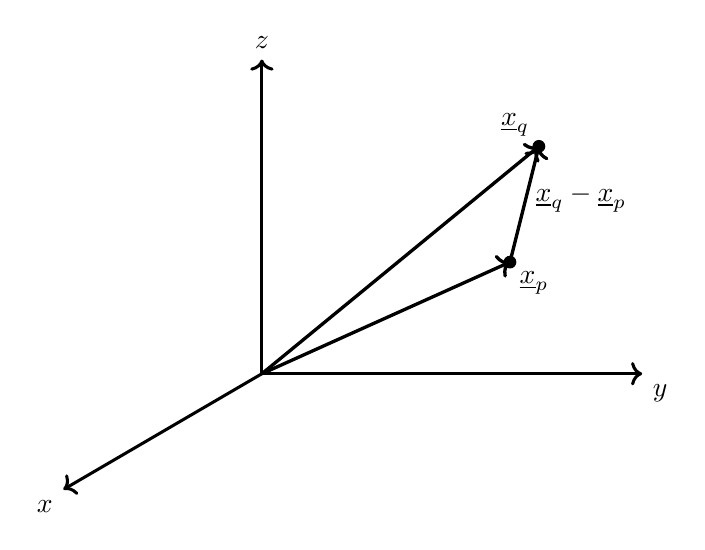
\begin{tikzpicture}[scale=1.05, line cap=round, line join=round]

% assi in prospettiva
\coordinate (O) at (0,0);
\draw[->,line width=1.1pt] (O) -- (-2.4,-1.4) node[below left] {$x$};
\draw[->,line width=1.1pt] (O) -- (4.6,0) node[below right] {$y$};
\draw[->,line width=1.1pt] (O) -- (0,3.8) node[above] {$z$};

% punti
\coordinate (Xp) at (3.0,1.35);
\coordinate (Xq) at (3.35,2.75);

% vettori posizione
\draw[->,line width=1.2pt] (O) -- (Xp);
\draw[->,line width=1.2pt] (O) -- (Xq);

% vettore differenza x_q - x_p
\draw[->,line width=1.2pt] (Xp) -- (Xq);

% punti marcati
\fill (Xp) circle (2.2pt);
\fill (Xq) circle (2.2pt);

% etichette
\node[below right] at (Xp) {$\underline{x}_p$};
\node[above left]  at (Xq) {$\underline{x}_q$};
\node[right] at ($(Xp)!0.55!(Xq)$) {$\underline{x}_q-\underline{x}_p$};

\end{tikzpicture}
\end{center}

determiniamo la velocità:
\[
(\underline{x}_q-\underline{x}_p)(t)=R\bigl(\underline{x}_q(0)-\underline{x}_p(0)\bigr)
\]
\[
\Rightarrow\quad
R^{\mathsf T}(\underline{x}_q-\underline{x}_p)(t)=\underline{x}_q(0)-\underline{x}_p(0)
\]
\[
\Rightarrow\quad
\frac{d\underline{x}_q}{dt}(t)=\frac{d\underline{x}_p}{dt}+\frac{d}{dt}\Bigl(R\bigl(\underline{x}_q(0)-\underline{x}_p(0)\bigr)\Bigr)
\]
\[
\Rightarrow\quad
\underline{v}_q=\underline{v}_p+\dot{R}R^{\mathsf T}(\underline{x}_q-\underline{x}_p).
\]
(dove $R=(r_{ij})$)

\medskip

$R(t)$ e $R^{\mathsf T}(t)$ sono funzioni del tempo e $RR^{\mathsf T}=I$.
Quindi
\[
\frac{d}{dt}(RR^{\mathsf T})=0
\ \Longleftrightarrow\
\dot{R}R^{\mathsf T}+R\dot{R}^{\mathsf T}=0
\ \Longleftrightarrow\
\dot{R}R^{\mathsf T}=-R\dot{R}^{\mathsf T}=-(\dot{R}R^{\mathsf T})^{\mathsf T}.
\]
\[
\Rightarrow\quad \dot{R}R^{\mathsf T}\ \text{è antisimmetrica, cioè}\quad
\dot{R}R^{\mathsf T}=
\begin{pmatrix}
0 & -\omega_z & \omega_y\\
\omega_z & 0 & -\omega_x\\
-\omega_y & \omega_x & 0
\end{pmatrix}.
\]

Quindi la velocità si può scrivere come
\[
\underline{v}_q=\underline{v}_p+
\begin{pmatrix}
0 & -\omega_z & \omega_y\\
\omega_z & 0 & -\omega_x\\
-\omega_y & \omega_x & 0
\end{pmatrix}
\begin{pmatrix}
x_q-x_p\\
y_q-y_p\\
z_q-z_p
\end{pmatrix}
=
\underline{v}_p+
\begin{pmatrix}
\omega_y(z_q-z_p)-\omega_z(y_q-y_p)\\
\omega_z(x_q-x_p)-\omega_x(z_q-z_p)\\
\omega_x(y_q-y_p)-\omega_y(x_q-x_p)
\end{pmatrix}.
\]

\[
\underline{v}_q=\underline{v}_p+\underline{\omega}\wedge(\underline{x}_q-\underline{x}_p),
\qquad
\underline{\omega}=
\begin{pmatrix}
\omega_x\\
\omega_y\\
\omega_z
\end{pmatrix}
\quad\text{(velocità angolare).}
\]

\[
\text{\emph{Formula fondamentale del moto dei corpi rigidi}.}
\]

\begin{oss}{}
$\underline{x}_p$ e $\underline{x}_q$ sono due punti qualsiasi del corpo rigido.
\end{oss}

\begin{oss}{}
In generale $\underline{\omega}=\bigl(\omega_x(t),\omega_y(t),\omega_z(t)\bigr)$, ma se vincoliamo il moto nel piano allora
\[
\underline{\omega}=(0,0,\omega(t)).
\]
\end{oss}
Possiamo derivare nel tempo la formula fondamentale ottenendo
\[
\frac{d}{dt}\left(\underline{v_q}\right)
=
\frac{d}{dt}\left(\underline{v_p}\right)
+
\frac{d}{dt}\left(\underline{\omega}\wedge\left(\underline{x_q}-\underline{x_p}\right)\right)
=
\]

\[
=
\underline{a_p}
+
\frac{d}{dt}\left(\underline{\omega}\right)\wedge\left(\underline{x_q}-\underline{x_p}\right)
+
\underline{\omega}\wedge\frac{d}{dt}\left(\underline{x_q}-\underline{x_p}\right)
=
\]

\[
=
\underline{a_p}
+
\underline{\alpha}\wedge\left(\underline{x_q}-\underline{x_p}\right)
+
\underline{\omega}\wedge\left(\underline{v_q}-\underline{v_p}\right)
=
\]

\[
=
\underline{a_p}
+
\underline{\alpha}\wedge\left(\underline{x_q}-\underline{x_p}\right)
+
\underline{\omega}\wedge\left(\underline{v_p}+\underline{\omega}\wedge\left(\underline{x_q}-\underline{x_p}\right)-\underline{v_p}\right)
=
\]

\[
=
\underline{a_p}
+
\underline{\alpha}\wedge\left(\underline{x_q}-\underline{x_p}\right)
+
\underline{\omega}\wedge\left(\underline{\omega}\wedge\left(\underline{x_q}-\underline{x_p}\right)\right)
\]
ovvero

\[
\underline{a_q}
=
\underline{a_p}
+
\underline{\alpha}\wedge\left(\underline{x_q}-\underline{x_p}\right)
+
\underline{\omega}\wedge\left(\underline{\omega}\wedge\left(\underline{x_q}-\underline{x_p}\right)\right)
\]

\chapter{Moti piani}
Un moto piano di un corpo rigido è caratterizzato dai vincoli
\[
\omega_x=\omega_y=0
\]
\[
z_p=k\in\mathbb{R}\qquad \forall\, p \in\mathcal{R}
\]

In particolare mostriamo che i vincoli olonomi
\[
\omega_x=\omega_y=0
\]
\[
z_q=0,\qquad q\in\mathcal{R}
\]
bastano per descrivere il sistema. Sia $p$ un punto del corpo rigido che ha componente $z_p=0$ nel nostro sistema di riferimento scelto. Sia $q$ un altro punto del corpo rigido. Mostriamo che $z_q=k\in\mathbb{R}$. Impostando la legge fondamentale si ottiene
\[
\underline{v}_q=\underline{v}_p+\underline{\omega}\wedge(\underline{x}_q-\underline{x}_p)
\]
e applicando i vincoli $z_p=0$, $\omega_x=\omega_y=0$ si ha
\[
\underline{\omega}=
\begin{pmatrix}
0\\
0\\
\omega_z
\end{pmatrix},
\qquad
\underline{x}_p=
\begin{pmatrix}
x_p\\
y_p\\
0
\end{pmatrix},
\qquad
\underline{x}_q=
\begin{pmatrix}
x_q\\
y_q\\
z_q
\end{pmatrix}
\]
\[
\underline{v}_p=
\begin{pmatrix}
v_{p,x}\\
v_{p,y}\\
0
\end{pmatrix},
\qquad
\underline{v}_q=
\begin{pmatrix}
v_{q,x}\\
v_{q,y}\\
v_{q,z}
\end{pmatrix}
\]
da cui
\[
\underline{v}_q=
\begin{pmatrix}
v_{q,x}\\
v_{q,y}\\
v_{q,z}
\end{pmatrix}
=
\begin{pmatrix}
v_{p,x}\\
v_{p,y}\\
0
\end{pmatrix}
+
\begin{pmatrix}
0\\
0\\
\omega_z
\end{pmatrix}
\wedge
\begin{pmatrix}
x_q-x_p\\
y_q-y_p\\
z_q
\end{pmatrix}
=
\]
\[
=
\begin{pmatrix}
v_{p,x}\\
v_{p,y}\\
0
\end{pmatrix}
+
\begin{vmatrix}
\hat{\imath} & \hat{\jmath} & \hat{k}\\
0 & 0 & \omega_z\\
x_q-x_p & y_q-y_p & z_q
\end{vmatrix}
=
\begin{pmatrix}
v_{p,x}\\
v_{p,y}\\
0
\end{pmatrix}
+\hat{\imath}\bigl(-\omega_z(y_q-y_p)\bigr)
+\hat{\jmath}\bigl(\omega_z(x_q-x_p)\bigr)
+\hat{k}\cdot 0
\]
\[
=
\begin{pmatrix}
v_{p,x}\\
v_{p,y}\\
0
\end{pmatrix}
+
\begin{pmatrix}
\omega_z y_p-\omega_z y_q\\
\omega_z x_q-\omega_z x_p\\
0
\end{pmatrix}
=
\begin{pmatrix}
v_{p,x}+\omega_z y_p-\omega_z y_q\\
v_{p,y}+\omega_z x_q-\omega_z x_p\\
0
\end{pmatrix}.
\]

In particolare
\[
v_{q,z}=0 \;\;\Rightarrow\;\; z_q=k\in\mathbb{R}.
\]
Un corpo rigido vincolato ad un moto piano ha quindi $6-3=3$ gradi di libertà.\\
Possiamo ad esempio descriverlo attraverso le coordinate libere
\[
x_{p}(t) , y_{p}(t) , w_z(t)  \quad p \in \mathcal{R}
\]

\begin{examplebreak}{}
Consideriamo un'asta rigida con un estremo $O$ vincolato nell'origine degli assi e costretto ad un moto piano.

\begin{figure}
\begin{tikzpicture}[scale=1.2]
    % assi
    \draw[->] (0,-3.2) -- (0,1.2) node[above] {$y$};
    \draw[->] (-0.2,0) -- (3.4,0) node[right] {$x$};

    % origine
    \fill (0,0) circle (2pt);
    \node[below left] at (0,0) {$O$};

    % asta
    \coordinate (P) at (1.55,-2.35);
    \draw[line width=0.9pt] (0,0) -- (P);

    % punto P
    \fill (P) circle (2pt);
    \node[right] at (P) {$P$};

    % arco theta
    \draw[->] (0,-1.15) arc[start angle=-90,end angle=-56,radius=1.15];
    \node[left] at (0.33,-1.45) {$\theta$};

    % arco l

    \node[right] at (1.1,-1.05) {$l$};

    % velocità vp
    \draw[->,red,line width=0.9pt] (P) -- ++(1.2,0.75);
    \node[red,right] at (2.75,-1.58) {$\underline{v}_p$};
\end{tikzpicture}
\end{figure}

Oltre ai vincoli del moto piano possiamo impostare
\[
x_O(t)=y_O(t)=0.
\]

Il corpo rigido ha quindi $3-2=1$ grado di libertà. Scegliamo come coordinata libera $\theta(t)$, l'angolo formato dall'asta con l'asse $y$, come illustrato in figura.

Impostiamo la legge fondamentale con $q=O$, da cui
\[
\underline{x}_q=
\begin{pmatrix}
0\\
0\\
0
\end{pmatrix},
\qquad
\underline{v}_q=\underline{0},
\]
e quindi
\[
\underline{v}_p=\underline{v}_q+\underline{\omega}\wedge(\underline{x}_p-\underline{x}_q)
=\underline{\omega}\wedge \underline{x}_p.
\]

Tenendo in considerazione che
\[
\underline{\omega}=
\begin{pmatrix}
0\\
0\\
\dot{\theta}
\end{pmatrix},
\qquad
\underline{x}_p=
\begin{pmatrix}
x_p\\
y_p\\
0
\end{pmatrix},
\]
allora
\[
\underline{v}_p=
\begin{pmatrix}
0\\
0\\
\dot{\theta}
\end{pmatrix}
\wedge
\begin{pmatrix}
x_p\\
y_p\\
0
\end{pmatrix}
=
\begin{vmatrix}
\hat{\imath} & \hat{\jmath} & \hat{k}\\
0 & 0 & \dot{\theta}\\
x_p & y_p & 0
\end{vmatrix}
=
\hat{\imath}(-y_p\dot{\theta})-\hat{\jmath}(-x_p\dot{\theta}),
\]
cioè
\[
\underline{v}_p=
\begin{pmatrix}
-y_p\dot{\theta}\\
x_p\dot{\theta}\\
0
\end{pmatrix}.
\]

Pertanto
\[
\underline{v}_p=(-y_p\dot{\theta},\,x_p\dot{\theta},\,0)^T
=
\|\underline{\omega}\|\,\|\underline{x}_p\|\,\hat{u}_{\perp}
=
l\,|\dot{\theta}|\,\hat{u}_{\perp},
\]
dove nell'ultimo passaggio
\[
l=\left\|
\begin{pmatrix}
x_p\\
y_p
\end{pmatrix}
\right\|
=d\!\left(
\begin{pmatrix}
x_p\\
y_p
\end{pmatrix},
\underline{0}\right)
\]
è costante perché il corpo è rigido e vincolato.

Nel penultimo passaggio abbiamo usato la regola della mano destra e la relazione
\[
\|\underline{v}_1\wedge \underline{v}_2\|
=
\|\underline{v}_1\|\,\|\underline{v}_2\|\sin\varphi.
\]
\end{examplebreak}
\begin{examplebreak}{}
Consideriamo ora una situazione fisica simile al precedente esempio. Questa volta però l'estremo $O$ dell'asta non è vincolato nell'origine degli assi, ma è mobile su una guida orizzontale posta lungo l'asse $x$.

\begin{figure}
\begin{tikzpicture}[scale=1.2]
    % assi
    \draw[->] (-0.8,0) -- (5.6,0) node[right] {$x$};
    \draw[->] (0,-3.2) -- (0,1.2) node[above] {$y$};

    % guida orizzontale
    \draw[line width=0.9pt] (0.9,0) -- (5.1,0);
    \node at (4.55,0.55) {\small guida orizzontale};

    % punto O
    \coordinate (O) at (2.0,0);
    \fill (O) circle (2pt);
    \node[above right] at (O) {$O$};

    % punto P
    \coordinate (P) at (3.2,-1.6);
    \fill (P) circle (2pt);
    \node[below left] at (P) {$P$};

    % asta
    \draw[line width=0.9pt] (O) -- (P);

    % proiezioni tratteggiate
    \draw[dashed] (O) -- (2.0,-2.6);
    \draw[dashed] (P) -- (3.2,0);
    \draw[dashed] (P) -- (5.0,-1.6);

    % etichetta s
    \node at (2.72,-0.78) {$s$};

    % arco theta a sinistra
    \draw[->] (2.0,-0.8) arc[start angle=-90,end angle=-53,radius=0.8];
    \node at (2.28,-1.15) {$\theta$};

    % arco theta a destra
    \draw[->] (3.85,-1.6) arc[start angle=0,end angle=37,radius=0.65];
    \node at (3.95,-1.15) {$\theta$};

    % velocità
    \draw[->,red,line width=0.9pt] (P) -- ++(1.0,0.75);
    \node[red,right] at (4.18,-0.95) {$\hat{u}_\perp$};

    % etichette varie
    \node at (2.45,0.6) {\small cerniera};
\end{tikzpicture}
\end{figure}

L'asta è soggetta quindi ai vincoli del moto piano e al vincolo
\[
y_O(t)=0.
\]

Ha dunque $3-1=2$ gradi di libertà. Usiamo le coordinate libere $x_O(t)$ e $\theta(t)$, ovvero la posizione lungo l'asse $x$ di $O$ e l'angolo $\theta(t)$ analogo all'esempio precedente.

Supponiamo $x_O(t)$ e $\theta(t)$ noti. Determiniamo $\underline{v}_p(t)$ per ogni $p$ e per ogni $t$.

Per la legge fondamentale della cinematica del corpo rigido,
\[
\underline{v}_p(t)=\underline{v}_O+\underline{\omega}\wedge(\underline{x}_p-\underline{x}_O).
\]

Poiché il moto è piano,
\[
\underline{\omega}=
\begin{pmatrix}
0\\
0\\
\dot{\theta}(t)
\end{pmatrix},
\qquad
\underline{v}_O=
\begin{pmatrix}
\dot{x}_O(t)\\
0\\
0
\end{pmatrix}.
\]

Inoltre
\[
\underline{x}_p-\underline{x}_O=
\begin{pmatrix}
x_p-x_O\\
y_p\\
0
\end{pmatrix}.
\]

Allora
\[
\underline{v}_p(t)=
\begin{pmatrix}
\dot{x}_O(t)\\
0\\
0
\end{pmatrix}
+
\begin{pmatrix}
0\\
0\\
\dot{\theta}(t)
\end{pmatrix}
\wedge
\begin{pmatrix}
x_p-x_O\\
y_p\\
0
\end{pmatrix}.
\]

Sviluppando il prodotto vettoriale,
\[
\underline{v}_p(t)=
\begin{pmatrix}
\dot{x}_O(t)\\
0\\
0
\end{pmatrix}
+
\begin{vmatrix}
\hat{\imath} & \hat{\jmath} & \hat{k}\\
0 & 0 & \dot{\theta}(t)\\
x_p-x_O & y_p & 0
\end{vmatrix}
=
\begin{pmatrix}
\dot{x}_O(t)-y_p\dot{\theta}(t)\\
(x_p-x_O)\dot{\theta}(t)\\
0
\end{pmatrix}.
\]

Quindi
\[
\underline{v}_p(t)
=
\dot{x}_O(t)\,\hat{\imath}
-y_p\dot{\theta}(t)\,\hat{\imath}
+(x_p-x_O)\dot{\theta}(t)\,\hat{\jmath}.
\]

Se indichiamo con
\[
s=
d\!\left(
\begin{pmatrix}
x_p\\
y_p
\end{pmatrix},
\begin{pmatrix}
x_O\\
0
\end{pmatrix}
\right)
\]
la distanza tra $P$ e $O$, che è costante perché l'asta è rigida, allora il termine rotazionale può essere scritto come
\[
s\,\dot{\theta}\,\hat{u}_\perp.
\]

Pertanto si ottiene
\[
\underline{v}_p(t)=\dot{x}_O(t)\,\hat{\imath}+s\,\dot{\theta}\,\hat{u}_\perp.
\]
\end{examplebreak}

\section{Moto di puro rotolamento}
\begin{definition}{}
Diciamo che due corpi rigidi che sono in contatto in un punto $P$ sono sottoposti ad un \emph{vincolo di puro rotolamento} se
\[
{}^{1}\underline{v}_P(t) = {}^{2}\underline{v}_P(t),
\]
dove ${}^{1}\underline{v}_P(t)$ è la velocità del punto di contatto $P$ vista dal corpo $1$ e ${}^{2}\underline{v}_P(t)$ è la velocità dello stesso punto vista dal corpo $2$.
\end{definition}

\begin{oss}{}
\begin{center}
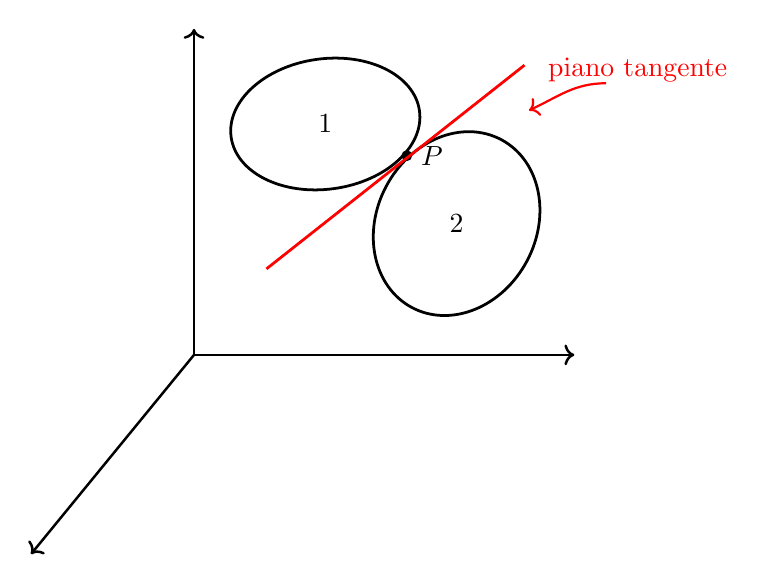
\begin{tikzpicture}[scale=1.15]

% terna cartesiana
\draw[->, line width=0.9pt] (0,0) -- (4.2,0);
\draw[->, line width=0.9pt] (0,0) -- (0,3.6);
\draw[->, line width=0.9pt] (0,0) -- (-1.8,-2.2);

% corpi rigidi stilizzati
\draw[line width=1pt] (1.45,2.55) ellipse [x radius=1.05, y radius=0.72, rotate=8];
\draw[line width=1pt] (2.9,1.45) ellipse [x radius=0.88, y radius=1.05, rotate=-28];

% punto di contatto
\fill (2.35,2.2) circle (1.7pt);
\node[right] at (2.4,2.2) {$P$};

% etichette corpi
\node at (1.45,2.55) {$1$};
\node at (2.9,1.45) {$2$};

% piano tangente (rappresentato da una retta nel disegno)
\draw[red, line width=1pt] (0.8,0.95) -- (3.65,3.2);
\node[red] at (4.9,3.15) {piano tangente};
\draw[red,->,line width=0.8pt] (4.55,3.0) to[out=180,in=25] (3.7,2.7);

\end{tikzpicture}
\end{center}

In un punto di contatto $P$ fra due corpi rigidi, le componenti delle velocità dei due corpi perpendicolari al piano tangente in $P$ devono essere concordi. In caso contrario, i due corpi tenderebbero a compenetrarsi, il che è incompatibile con il vincolo di contatto.
\end{oss}

\begin{examplebreak}{}
Moto di un disco in un piano orizzontale fermo.

\begin{figure}
\centering
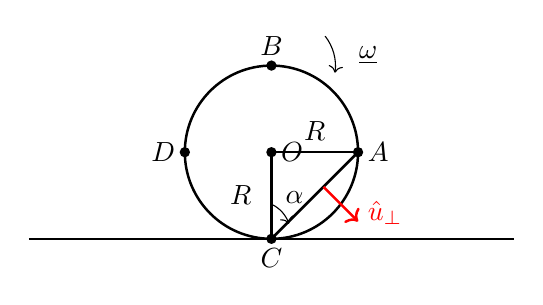
\begin{tikzpicture}[scale=1.1]
    % piano
    \draw[line width=0.9pt] (-2.8,0) -- (2.8,0);

    % disco
    \draw[line width=0.9pt] (0,1) circle (1);

    % punti
    \fill (0,1) circle (1.7pt);
    \fill (1,1) circle (1.7pt);
    \fill (0,0) circle (1.7pt);
    \fill (0,2) circle (1.7pt);
    \fill (-1,1) circle (1.7pt);

    \node[right] at (0,1) {$O$};
    \node[right] at (1,1) {$A$};
    \node[below] at (0,0) {$C$};
    \node[above] at (0,2) {$B$};
    \node[left] at (-1,1) {$D$};

    % raggi
    \draw[line width=0.9pt] (0,1) -- (1,1);
    \draw[line width=0.9pt] (0,1) -- (0,0);
    \draw[line width=0.9pt] (0,0) -- (1,1);

    % etichette
    \node[left] at (-0.12,0.5) {$R$};
    \node[above] at (0.5,1.02) {$R$};

    % angolo alpha
    \draw[->] (0,0.4) arc[start angle=65,end angle=18,radius=0.38];
    \node[right] at (0.05,0.48) {$\alpha$};

    % omega
    \draw[->] (0.62,2.34) arc[start angle=38,end angle=-8,radius=0.56];
    \node[right] at (0.9,2.12) {$\underline{\omega}$};

    % u_perp
    \draw[->,red,line width=0.9pt] (0.6,0.6) -- (1,0.2);
    \node[red,right] at (1,0.3) {$\hat{u}_{\perp}$};
\end{tikzpicture}
\end{figure}

Chiamiamo $C$ il punto di contatto con il piano al tempo $t$.

Impongo $\underline{v}_C(t)=0$. Toglie $2$ gradi di libertà e ne resta $1$.

Descriviamo il moto usando
\[
\underline{\omega}=\dot{\theta}\,\hat{k}.
\]

Definisco $\underline{\omega}$ positivo in senso orario (uso $(0,0,-1)^T$
nella base).

Scelgo di utilizzare la formula fondamentale del moto dei corpi rigidi con $x_q=x_C$.
Sotto ipotesi di puro rotolamento $\underline{v}_C=(0,0,0)$.
Calcoliamo la velocità di $O$.
\[
\underline{v}_O=0+R\dot{\theta}\,\hat{\imath}
\qquad
\underline{v}_B=0+2R\dot{\theta}\,\hat{\imath}
\]

\[
\underline{v}_A=\underline{v}_O+\underline{\omega}\wedge(\underline{x}_A-\underline{x}_O)
=R\dot{\theta}\,\hat{\imath}-\dot{\theta}R\,\hat{\jmath}
=\dot{\theta}R(\hat{\imath}-\hat{\jmath})
=
\dot{\theta}R
\begin{pmatrix}
1\\
-1\\
0
\end{pmatrix}
\]
\[
\underline{v}_D=R\dot{\theta}\,\hat{\imath}+R\dot{\theta}\,\hat{\jmath}
=
R\dot{\theta}
\begin{pmatrix}
1\\
1\\
0
\end{pmatrix}
\]

Possiamo anche calcolare $\underline{v}_A$ a partire da $C$.
\[
\underline{v}_A=
\underline{\omega}\wedge(\underline{x}_A-\underline{x}_C)
=
-\frac{R}{\sin\alpha}\,\dot{\theta}\,\hat{\jmath}
=
\sqrt{2}\,R\dot{\theta}\,\hat{u}_{\perp}
=
\sqrt{2}\,R\dot{\theta}
\begin{pmatrix}
\frac{1}{\sqrt{2}}\\[4pt]
-\frac{1}{\sqrt{2}}\\[4pt]
0
\end{pmatrix}
=
R\dot{\theta}
\begin{pmatrix}
1\\
-1\\
0
\end{pmatrix}
\]
\end{examplebreak}

\begin{examplebreak}{}
Consideriamo un disco che rotola senza strisciare su un carrello che trasla orizzontalmente.

\begin{figure}
\begin{tikzpicture}[scale=1.15]
    % assi
    \draw[->] (-0.3,0) -- (6.4,0) node[right] {$x$};
    \draw[->] (0,-0.3) -- (0,3.8) node[above] {$y$};

    % carrello appoggiato sull'asse x
    \draw[line width=0.9pt] (1.2,0) -- (5.4,0);
    \fill (1.5,0) circle (1.6pt);
    \fill (5.1,0) circle (1.6pt);
    \node[above] at (1.5,0) {$A$};
    \node[above] at (5.1,0) {$B$};

    % piedini/ruote simmetrici e dritti sotto il carrello
    \draw[line width=0.9pt] (2.2,0) -- (2.05,-0.22) -- (2.35,-0.22) -- cycle;
    \draw[line width=0.9pt] (4.2,0) -- (4.05,-0.22) -- (4.35,-0.22) -- cycle;

    % disco tangente al carrello
    \def\R{1}
    \coordinate (C) at (3.3,0);
    \coordinate (O) at (3.3,1.0);
    \draw[line width=0.9pt] (O) circle (\R);

    % centro e punto di contatto
    \fill (O) circle (1.5pt);
    \fill (C) circle (1.5pt);
    \node[right] at (3.35,1.02) {$O$};
    \node[below] at (3.3,-0.02) {$C$};
\end{tikzpicture}
\end{figure}

Abbiamo due corpi rigidi, quindi in totale $6$ gradi di libertà.

I vincoli sono:
\[
y_A=0,\qquad y_B=0,
\]
e il vincolo di puro rotolamento nel punto di contatto $C$,
\[
\underline{v}_C^{\text{disco}}=\underline{v}_C^{\text{carrello}}.
\]

In totale otteniamo $4$ vincoli, dunque rimangono
\[
6-4=2
\]
gradi di libertà.

Scegliamo come coordinate libere
\[
x_A,\qquad \theta.
\]

Applicando la formula fondamentale della cinematica del corpo rigido al disco, con polo in $C$, si ha
\[
\underline{v}_O=\underline{v}_C+\underline{\omega}\wedge(\underline{x}_O-\underline{x}_C).
\]
Poiché il carrello trasla orizzontalmente,
\[
\underline{v}_C=\dot{x}_A\,\hat{\imath},
\]
mentre, essendo
\[
\underline{\omega}=\dot{\theta}\,\hat{k},
\qquad
\underline{x}_O-\underline{x}_C=R\,\hat{\jmath},
\]
segue
\[
\underline{v}_O=\dot{x}_A\,\hat{\imath}+\dot{\theta}\,\hat{k}\wedge R\,\hat{\jmath}
=\dot{x}_A\,\hat{\imath}+R\dot{\theta}\,\hat{\imath}.
\]
Quindi
\[
\underline{v}_O=(\dot{x}_A+R\dot{\theta})\,\hat{\imath}.
\]
\end{examplebreak}

\begin{oss}{}
Il vincolo di puro rotolamento in questo caso è integrabile.
\end{oss}
\begin{oss}{}
    Sull'asse verticale del disco la velocità dovuta al puro rotolamento aumenta linearmente con la distanza da C.
    \begin{center}
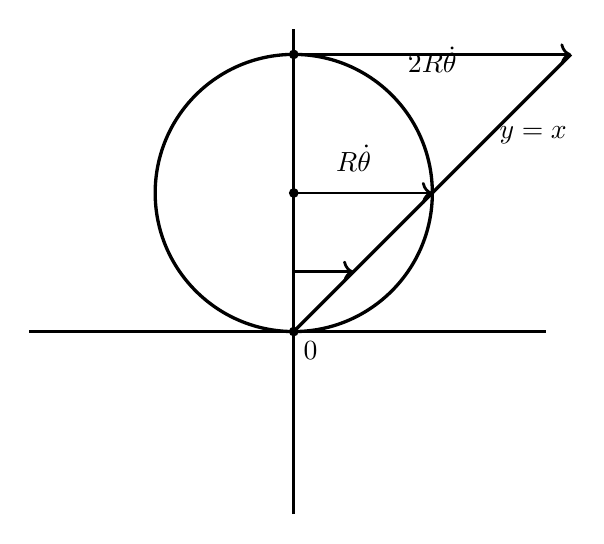
\begin{tikzpicture}[scale=0.8]
    % parametri
    \def\R{2.2}
    \pgfmathsetmacro{\rt}{sqrt(2)*\R}

    % piano orizzontale
    \draw[line width=1.1pt] (-4.2,0) -- (4.0,0);

    % asse verticale
    \draw[line width=1.1pt] (0,-2.9) -- (0,4.8);

    % disco
    \draw[line width=1.2pt] (0,\R) circle (\R);

    % punti notevoli
    \fill (0,0) circle (2.2pt);
    \node[below right] at (0,0) {$0$};

    \fill (0,\R) circle (2.2pt);
    \fill (0,2*\R) circle (2.2pt);

    % retta obliqua
    \draw[line width=1.2pt] (0,0) -- ({\R * 2},{\R * 2});
    \node[right] at (\rt,\rt) {$y=x$};



    % frecce orizzontali
    \draw[->, line width=1pt] (0,0.95) -- (0.95,0.95);
    \draw[->, line width=1pt] (0,\R) -- ({\R},{\R});
    \draw[->, line width=1pt] (0,{\R * 2}) -- ({\R * 2},{\R * 2});

    % etichette
    \node at (0.95,\R+0.55) {$R\dot{\theta}$};
    \node[above] at (2.2,3.95) {$2R\dot{\theta}$};
\end{tikzpicture}
\end{center}
\end{oss}

\begin{theorem}{}
    La velocità angolare   è univocamente determinata dal moto del corpo rigido. In particolare non cambia da punto a punto del corpo rigido.
\end{theorem}
\begin{proof}
Siano $\underline{\omega}_1$ e $\underline{\omega}_2$ due vettori velocità angolare associati allo stesso atto di moto, valutati a partire da due poli di riferimento diversi $q_1$ e $q_2$.

Per un generico punto $p$ del corpo rigido possiamo scrivere:
\[
\underline{v}_p=\underline{v}_{q_1}+\underline{\omega}_1\wedge(\underline{x}_p-\underline{x}_{q_1})
\]
\[
\underline{v}_p=\underline{v}_{q_2}+\underline{\omega}_2\wedge(\underline{x}_p-\underline{x}_{q_2})
\]

Sottraiamo le 2 equazioni:
\[
\underline{0}=\underline{v}_{q_1}-\underline{v}_{q_2}
+\underline{\omega}_1\wedge(\underline{x}_p-\underline{x}_{q_1})
-\underline{\omega}_2\wedge(\underline{x}_p-\underline{x}_{q_2})
\]

Esprimiamo $\underline{v}_{q_2}$ rispetto a $q_1$ tramite la formula fondamentale:
\[
\underline{v}_{q_2}=\underline{v}_{q_1}+\underline{\omega}_1\wedge(\underline{x}_{q_2}-\underline{x}_{q_1})
\]

Sostituendo nell'espressione precedente:
\[
\underline{0}
=
\underline{v}_{q_1}
-
\Bigl(\underline{v}_{q_1}+\underline{\omega}_1\wedge(\underline{x}_{q_2}-\underline{x}_{q_1})\Bigr)
+\underline{\omega}_1\wedge(\underline{x}_p-\underline{x}_{q_1})
-\underline{\omega}_2\wedge(\underline{x}_p-\underline{x}_{q_2})
\]

Sviluppando i prodotti vettoriali:
\[
\Rightarrow\quad
\underline{0}
=
-\underline{\omega}_1\wedge \underline{x}_{q_2}
+\underline{\omega}_1\wedge \underline{x}_{q_1}
+\underline{\omega}_1\wedge \underline{x}_p
-\underline{\omega}_1\wedge \underline{x}_{q_1}
-\underline{\omega}_2\wedge \underline{x}_p
+\underline{\omega}_2\wedge \underline{x}_{q_2}
\]

Semplificando i termini opposti:
\[
\Rightarrow\quad
\underline{0}
=
-\underline{\omega}_1\wedge \underline{x}_{q_2}
+\underline{\omega}_1\wedge \underline{x}_p
-\underline{\omega}_2\wedge \underline{x}_p
+\underline{\omega}_2\wedge \underline{x}_{q_2}
\]

Raccogliendo a fattor comune i prodotti vettoriali:
\[
\Rightarrow\quad
\underline{0}
=
\underline{\omega}_1\wedge(\underline{x}_p-\underline{x}_{q_2})
-\underline{\omega}_2\wedge(\underline{x}_p-\underline{x}_{q_2})
\]

\[
\Rightarrow\quad
\underline{0}
=
(\underline{\omega}_1-\underline{\omega}_2)\wedge(\underline{x}_p-\underline{x}_{q_2})
\qquad \forall\,\underline{x}_p
\]

Poiché questa relazione deve valere per ogni punto $p$, e quindi per un generico vettore $(\underline{x}_p-\underline{x}_{q_2})$, l'unica soluzione possibile affinché il prodotto vettoriale sia sempre nullo è che il primo fattore sia nullo:
\[
\Rightarrow\quad
\underline{\omega}_1-\underline{\omega}_2=0
\iff
\underline{\omega}_1=\underline{\omega}_2
\]
\end{proof}

\begin{example}{}
\begin{center}
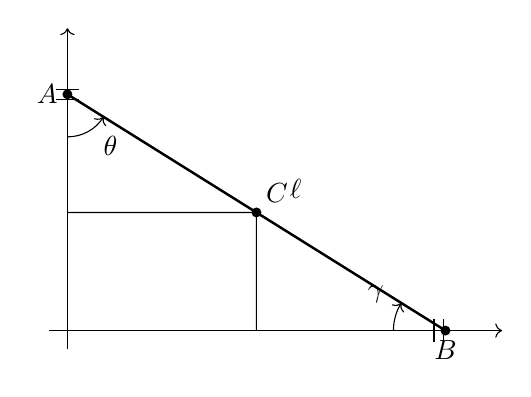
\begin{tikzpicture}[scale=1.2]
    % assi
    \draw[->] (-0.2,0) -- (4.6,0);
    \draw[->] (0,-0.2) -- (0,3.2);

    % punti
    \coordinate (A) at (0,2.5);
    \coordinate (B) at (4,0);
    \coordinate (C) at (2,1.25);

    % asta
    \draw[line width=0.9pt] (A) -- (B);

    % proiezioni di C
    \draw (C) -- (0,1.25);
    \draw (C) -- (2,0);

    % punti marcati
    \fill (A) circle (1.5pt);
    \fill (B) circle (1.5pt);
    \fill (C) circle (1.5pt);

    % etichette
    \node[left] at (A) {$A$};
    \node[below] at (B) {$B$};
    \node[above right] at (C) {$C$};
    \node[right] at (2.25,1.5) {$\ell$};

    % vincoli in A e B
    \draw (-0.12,2.55) -- (0.12,2.55);
    \draw (-0.12,2.45) -- (0.12,2.45);

    \draw (3.88,-0.12) -- (3.88,0.12);
    \draw (3.98,-0.12) -- (3.98,0.12);

    % angolo theta
    \draw[->] (0,2.05) arc[start angle=-90,end angle=-32,radius=0.45];
    \node[right] at (0.28,1.95) {$\theta$};

    % angolo gamma
    \draw[->] (3.45,0) arc[start angle=180,end angle=148,radius=0.55];
    \node[left] at (3.45,0.38) {$\gamma$};
\end{tikzpicture}
\end{center}

I vincoli sono
\[
\begin{cases}
x_A=0 \qquad \forall t,\\
y_B=0 \qquad \forall t,
\end{cases}
\]
da cui si ha $3-2 = 1$ grado di libertà.

Come coordinata libera posso scegliere:
\[
\theta(t),\ \gamma(t),\ x_B(t),\ y_A(t),\ x_C(t),\ y_C(t).
\]

Usiamo $\theta(t)$.

\[
\begin{cases}
x_C=\dfrac{\ell}{2}\sin\theta,\\[6pt]
y_C=\dfrac{\ell}{2}\cos\theta
\end{cases}
\qquad \Longrightarrow \qquad
\underline{v}_C=
\begin{pmatrix}
\dfrac{\ell}{2}\cos\theta\,\dot{\theta}\\[6pt]
-\dfrac{\ell}{2}\sin\theta\,\dot{\theta}
\end{pmatrix}.
\]
\end{example}



\begin{example}{}
    Studiamo il seguente sistema
\begin{center}
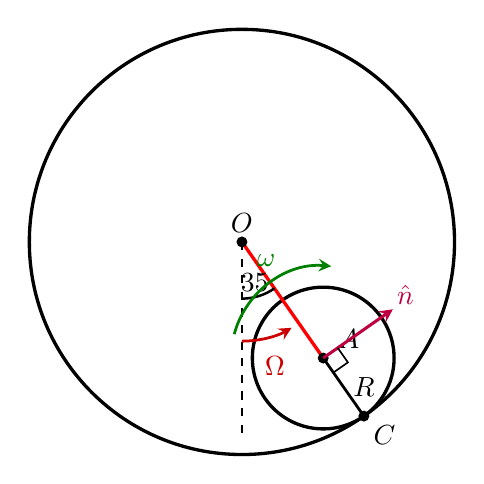
\begin{tikzpicture}[scale=0.9, >=stealth]

% parametri
\def\Rbig{3}
\def\Rsmall{1}
\def\theta{35} % angolo dal verticale verso destra

% centri (usando le coordinate polari dirette di TikZ)
\coordinate (O) at (0,0);
\coordinate (A) at ({-90+\theta}:2*\Rsmall); % distanza 2R
\coordinate (C) at ({-90+\theta}:3*\Rsmall); % distanza 3R

% circonferenza fissa
\draw[line width=1.2pt] (O) circle (\Rbig);

% disco piccolo (riempito di bianco per coprire l'asse e pulire il disegno)
\draw[line width=1.2pt, fill=white] (A) circle (\Rsmall);

% segmento OA in rosso e AC in nero
\draw[red, line width=1.2pt] (O) -- (A);
\draw[line width=1pt] (A) -- (C);

% tratteggio verticale
\draw[dashed, thick] (O) -- (0,-2.8);

% punti
\fill (O) circle (2.2pt) node[above] {$O$};
\fill (A) circle (2.2pt) node[above right, xshift=2pt] {$A$};
\fill (C) circle (2.2pt) node[below right] {$C$};

% etichetta R
\node[right] at ($(A)!0.5!(C)$) {$R$};

% --- CORREZIONE VERSORE \hat{n} ---
% Disegnato perpendicolare all'asta, con il simbolo di angolo retto
\draw[->, line width=1.1pt, purple] (A) -- ++(\theta:1.2) node[above right, inner sep=1pt] {$\hat{n}$};
% Simboletto angolo retto
\draw[line width=0.6pt] ($(A)+({-90+\theta}:0.25)$) -- ++(\theta:0.25) -- ++({90+\theta}:0.25);


% --- CORREZIONE ROTAZIONI E ANGOLO ---
% angolo theta (minuscolo, coerente col testo!)
\draw[line width=0.9pt] (0,-0.8) arc[start angle=-90, end angle={-90+\theta}, radius=0.8];
\node at ({-90+\theta/2}:0.6) {$\theta$};

% freccia Omega dell'asta (ora abbraccia la cerniera in modo fluido)
\draw[->, line width=1pt, red!80!black] (0,-1.4) arc[start angle=-90, end angle={-90+\theta-5}, radius=1.4];
\node[red!80!black, below] at ({-90+\theta/2}:1.55) {$\Omega$};

% freccia omega del disco (ruota perfettamente attorno ad A)
\draw[->, line width=1pt, green!50!black] ($(A)+({90+\theta+40}:1.3)$) arc[start angle={90+\theta+40}, end angle={90+\theta-40}, radius=1.3];
\node[green!50!black, above] at ($(A)+(90+\theta:1.4)$) {$\omega$};

\end{tikzpicture}
\end{center}


Consideriamo una guida circolare fissa di raggio $3R$.

In $C$ imponiamo il puro rotolamento.

Chiamiamo
\begin{itemize}
    \item $\omega$ velocità angolare del disco,
    \item $\Omega$ velocità angolare dell'asta.
\end{itemize}

Ad una prima analisi verrebbe da imporre i $6$ vincoli
\begin{itemize}
    \item $x_O^{\text{asta}}=y_O^{\text{asta}}=0$,
    \item $\underline{v}_C=\underline{0}$,
    \item $x_A^{\text{asta}}(t)=x_A^{\text{disco}}(t)$,
    \item $y_A^{\text{asta}}(t)=y_A^{\text{disco}}(t)$,
\end{itemize}
che però non possono essere indipendenti, perché altrimenti il sistema avrebbe $0$ gradi di libertà.

Possiamo mostrare la dipendenza riscrivendo $\underline{v}_C$ nella base del diedro di Frenet associato alla guida.

Stiamo imponendo che
\[
\underline{v}_C=0\cdot \hat{\imath}+0\cdot \hat{\jmath}
\]
e cambiando base possiamo scrivere
\[
\underline{v}_C=0\cdot \underline{T}+0\cdot \underline{N}
\]
dal momento che il vettore nullo ha coordinate $(0,0)$ in ogni base.

A questo punto notiamo che l'insieme dei vincoli
\[
x_A^{\text{asta}}(t)=x_A^{\text{disco}}(t),
\qquad
y_A^{\text{asta}}(t)=y_A^{\text{disco}}(t),
\qquad
x_O^{\text{asta}}=y_O^{\text{asta}}=0
\]
già impongono che la componente lungo $\underline{n}$ di $\underline{v}_C$ sia nulla e quindi
\[
\underline{v}_C=\underline{0}
\]
dà solo $1$ vincolo aggiuntivo.

Il sistema ha dunque
\[
6-5=1
\]
grado di libertà.

Scelgo come coordinata libera l'angolo $\theta(t)$ che l'asta forma con il diametro verticale della guida.

Notiamo che
\[
\Omega=\dot{\theta}.
\]
Dobbiamo essere in grado di ricavare anche $\omega$ in funzione di $\dot{\theta}$.

\[
\underline{v}_A^{\text{asta}}
=
\underline{v}_O+\underline{\Omega}\wedge(\underline{x}_A-\underline{x}_O)
=
0+\Omega\,2R\,\hat{n}
\]

\[
\underline{v}_A^{\text{disco}}
=
\underline{v}_C+\underline{\omega}\wedge(\underline{x}_A-\underline{x}_C)
=
0+\omega R\,\hat{n}
\]

Usando
\[
\underline{x}_A^{\text{asta}}=\underline{x}_A^{\text{disco}}
\]
si ottiene
\[
\underline{v}_A^{\text{disco}}=\underline{v}_A^{\text{asta}}
\]
e quindi
\[
\omega R=2R\,\Omega
\quad\Rightarrow\quad
\omega=2\Omega=2\dot{\theta}.
\]
\end{example}

\chapter{Il Teorema di Mozzi}
Se in un moto di un corpo rigido poniamo
\[
\underline{\omega}=\text{cost.}
\]
allora esiste unico un asse di rotazione fisso. Possiamo avere due casi:

\begin{itemize}
    \item[(i)] i punti $q$ lungo l'asse di rotazione sono fermi
    \[
    \underline{v}_q=0
    \]
    e allora
    \[
    \underline{v}_p=\underline{\omega}\wedge(\underline{x}_p-\underline{x}_q).
    \]
    I punti del corpo rigido descrivono nello spazio traiettorie circolari di raggio uguale alla distanza di $\underline{x}_p$ dall'asse di rotazione.

    \item[(ii)] punti $\underline{x}_q$ lungo l'asse con velocità parallela all'asse.

    La traiettoria di $\underline{x}_p$ è un'elica; se $\underline{v}_q$ è costante l'elica è di passo fissato, altrimenti ha passo variabile.
\end{itemize}

\begin{lemma}{}
Dati due vettori $\underline{a} \ne \underline{0},\underline{b} \in \mathbb{R}^3$, se $\underline{a}\cdot \underline{b} = 0$ allora la relazione
\[
\underline{a}\wedge \underline{x}=\underline{b}
\]
individua una retta.
\end{lemma}
\begin{proof}
Fissiamo
\[
\underline{a}=(a_1,a_2,a_3)\in\mathbb{R}^3.
\]
Consideriamo l'applicazione lineare
\[
L:\mathbb{R}^3\to\mathbb{R}^3,
\qquad
\underline{x}\longmapsto \underline{a}\wedge \underline{x}.
\]

Rappresentiamo $L$ tramite una matrice $A\in\mathbb{R}^{3,3}$ attraverso la base canonica in partenza e in arrivo.
\[
A=\bigl([L(e_1)]_{\mathcal E},\ [L(e_2)]_{\mathcal E},\ [L(e_3)]_{\mathcal E}\bigr)
\]

\[
L(e_1)=
\begin{pmatrix}
a_1\\
a_2\\
a_3
\end{pmatrix}
\wedge
\begin{pmatrix}
1\\
0\\
0
\end{pmatrix}
=
\begin{vmatrix}
\hat{\imath} & \hat{\jmath} & \hat{k}\\
a_1 & a_2 & a_3\\
1 & 0 & 0
\end{vmatrix}
=
\hat{\jmath}(a_3)-\hat{k}(a_2)
=
\begin{pmatrix}
0\\
a_3\\
-a_2
\end{pmatrix}
\]

\[
L(e_2)=
\begin{pmatrix}
a_1\\
a_2\\
a_3
\end{pmatrix}
\wedge
\begin{pmatrix}
0\\
1\\
0
\end{pmatrix}
=
\begin{vmatrix}
\hat{\imath} & \hat{\jmath} & \hat{k}\\
a_1 & a_2 & a_3\\
0 & 1 & 0
\end{vmatrix}
=
-a_3\hat{\imath}+a_1\hat{k}
=
\begin{pmatrix}
-a_3\\
0\\
a_1
\end{pmatrix}
\]

\[
L(e_3)=
\begin{pmatrix}
a_1\\
a_2\\
a_3
\end{pmatrix}
\wedge
\begin{pmatrix}
0\\
0\\
1
\end{pmatrix}
=
\begin{vmatrix}
\hat{\imath} & \hat{\jmath} & \hat{k}\\
a_1 & a_2 & a_3\\
0 & 0 & 1
\end{vmatrix}
=
a_2\hat{\imath}-a_1\hat{\jmath}
=
\begin{pmatrix}
a_2\\
-a_1\\
0
\end{pmatrix}
\]

\[
\Rightarrow\quad
A=
\begin{pmatrix}
0 & -a_3 & a_2\\
a_3 & 0 & -a_1\\
-a_2 & a_1 & 0
\end{pmatrix}
\]

$L$ è quindi rappresentata da una matrice antisimmetrica ovvero
\[
A^T=-A
\iff
A=-A^T
\]

\[
\Rightarrow\quad
\det(A)=\det(A^T)=\det(-A^T)=-\det(A)
\iff
\det(A)=0
\]

Abbiamo quindi ottenuto che $L_A$ (e quindi $L$) non è una mappa iniettiva. Di conseguenza il nucleo di $L_A$ ha dimensione maggiore o uguale a $1$. Il caso
\[
\dim(\ker L_A)=3
\]
è assurdo perché implica
\[
\operatorname{Im}(L_A)=\{0\}
\]
ovvero
\[
\underline{a}=0.
\]
Il caso
\[
\dim(\ker L_A)=2
\]
è altrettanto problematico perché implica che
\[
\dim(\operatorname{Im}(L_A))=1
\]
ovvero che tutti i prodotti vettoriali di $\underline{a}$ con $\underline{x}\in\mathbb{R}^3$ stanno su una retta. Limitiamoci a
\[
\dim(\ker L_A)=1.
\]
Allora se
\[
\underline{b}\in\operatorname{Im}(L_A)
\]
le soluzioni di
\[
A\underline{x}=\underline{b}
\]
sono quindi un affine di $\ker(L_A)$ e quindi una retta.\\
Notiamo che per costruzione del prodotto vettoriale $\operatorname{Ker}(L) = \operatorname{span}(\underline{a})$ ovvero la  retta trovata è affine e con vettore direttore $\underline{a}$.\\
Notiamo infine che se $\underline{a} \ne \underline{0}$ allora
\[
\underline{b} \in \operatorname{Im}(L_A) \Leftrightarrow \underline{a} \cdot \underline{b} = 0
\]
per le proprietà del prodotto vettoriale
\end{proof}
\begin{oss}{}
Per trovare la retta individuata da
\[
\underline{a}\wedge \underline{x}=\underline{b}
\qquad \text{con } \underline{a}\neq \underline{0}
\quad \text{e} \quad
\underline{a}\cdot \underline{b}=0
\]
in forma parametrica possiamo procedere come segue.

Se
\[
L:\mathbb{R}^3\to\mathbb{R}^3,
\qquad
\underline{x}\mapsto \underline{a}\wedge \underline{x},
\]
allora
\[
L^{-1}(\{\underline{b}\})=\underline{x}_0+\ker(L)=\underline{x}_0+\mathrm{Span}\{\underline{a}\},
\qquad
\text{con } \underline{x}_0\in L^{-1}(\{\underline{b}\}).
\]

Per concludere basta notare che
\[
\underline{x}_0=-\frac{\underline{a}\wedge \underline{b}}{\|\underline{a}\|^2}
\]
fa al caso nostro. Infatti
\[
L\left(-\frac{\underline{a}\wedge \underline{b}}{\|\underline{a}\|^2}\right)
=
-\frac{1}{\|\underline{a}\|^2}\Bigl(\underline{a}\wedge(\underline{a}\wedge \underline{b})\Bigr)
=
-\frac{1}{\|\underline{a}\|^2}\Bigl(\underline{a}\,(\underline{a}\cdot \underline{b})-\underline{b}\,(\underline{a}\cdot \underline{a})\Bigr)
=
-\frac{1}{\|\underline{a}\|^2}\cdot\bigl(-\underline{b}\,\|\underline{a}\|^2\bigr)
=
\underline{b}.
\]

Dunque la retta si scrive in forma parametrica come
\[
\underline{x}_t=t\,\underline{a}-\frac{\underline{a}\wedge \underline{b}}{\|\underline{a}\|^2},
\qquad
t\in\mathbb{R}.
\]

\end{oss}

\begin{theorem}{}[di Mozzi]
    La traiettoria di un punto di un corpo rigido che si muove di un moto qualsiasi è istantaneamente elicoidale.
\end{theorem}
\begin{proof}
Per ogni moto possiamo scrivere
\[
\underline{v}_p=\underline{v}_q+\underline{\omega}\wedge(\underline{x}_p-\underline{x}_q)
\]

Decomponiamo lungo la direzione parallela e perpendicolare a $\underline{\omega}$
\[
\underline{v}_q=\underline{v}_q^{\parallel}+\underline{v}_q^{\perp}
\]

\[
\underline{v}_q^{\parallel}
=
\left(
\underline{v}_q\cdot
\left(
\frac{\underline{\omega}}{\|\underline{\omega}\|}
\right)
\right)
\frac{\underline{\omega}}{\|\underline{\omega}\|}
\]

\[
\underline{v}_q^{\perp}=\underline{v}_q-\underline{v}_q^{\parallel}
\]

L'idea è quella di riuscire a far vedere che il moto del generico punto $\underline{x}_q$ o $\underline{x}_p$ è composto da una velocità parallela all'asse di rotazione più una velocità perpendicolare all'asse che produca un moto circolare attorno l'asse stesso. Un punto dell'asse  $\underline{x}_r$ deve quindi soddisfare la seguente condizione che impone proprio la velocità di un moto circolare attorno all'asse.
\[
\underline{v}_q^{\perp}
=
\underline{\omega}\wedge(\underline{x}_q-\underline{x}_r)
\iff
\underline{\omega}\wedge \underline{x}_r
=
-\underline{v}_q^{\perp}
+
\underline{\omega}\wedge \underline{x}_q
\]

Per il lemma gli $\underline{x}_r$ individuano una retta affine di direzione $\underline{\omega}$. Sostituisco
\[
\underline{v}_q^{\perp}
=
\underline{\omega}\wedge(\underline{x}_q-\underline{x}_r)
\]
in
\[
\underline{v}_p=\underline{v}_q^{\parallel}+\underline{v}_q^{\perp}+\underline{\omega}\wedge(\underline{x}_p-\underline{x}_q)
\]

\[
\underline{v}_p
=
\underline{v}_q^{\parallel}
+
\underline{\omega}\wedge(\underline{x}_q-\underline{x}_r)
+
\underline{\omega}\wedge(\underline{x}_p-\underline{x}_q)
=
\]

\[
=
\underline{v}_q^{\parallel}
+
\underline{\omega}\wedge(\underline{x}_p-\underline{x}_r)
\]

Il moto trovato è un moto elicoidale e l'insieme dei punti $\{\underline{x}_r\}$ è detto asse di Mozzi.
\end{proof}
\begin{oss}{}
    $\underline{x_r}$ non è necessariamente un punto del corpo.
\end{oss}
\begin{oss}{}
La velocità $\underline{v}_{q}^{\parallel}$ usata a fine dimostrazione in
\[
\underline{v}_{p}=\underline{v}_{q}^{\parallel}+\underline{\omega}\wedge\left(\underline{x}_{p}-\underline{x}_{r}\right)
\]
è la velocità istantanea di ogni punto dell'asse. Infatti, se $\underline{x}_{p}=\underline{x}_{s}$ è un punto dell'asse, otteniamo
\[
\underline{v}_{s}=\underline{v}_{q}^{\parallel}+\underline{\omega}\wedge\left(\underline{x}_{s}-\underline{x}_{r}\right).
\]
E dal momento che
\[
\underline{x}_{s}-\underline{x}_{r}\parallel \underline{\omega}
\]
otteniamo
\[
\underline{v}_{s}=\underline{v}_{q}^{\parallel}.
\]

In particolare tutti i punti dell'asse di Mozzi hanno stessa velocità istantanea, che coincide con la proiezione della velocità di un qualsiasi punto $\underline{x}_{q}$ lungo l'asse.

\end{oss}
\begin{oss}{}
    La descrizione del moto non dipende dal punto dell'asse scelto. Infatti se $\underline{x_{r_1}}$ e $\underline{x_{r_2}}$ sono due punti dell'asse parallelo a $\underline{\omega}$ e $\underline{x_p}$ è un punto qualsiasi si ha che
    \[
        \underline{\omega} \wedge (\underline{x_p} - \underline{x_{r_1}}) =  \underline{\omega} \wedge (\underline{x_p} - \underline{x_{r_2}})
    \]

    \begin{center}
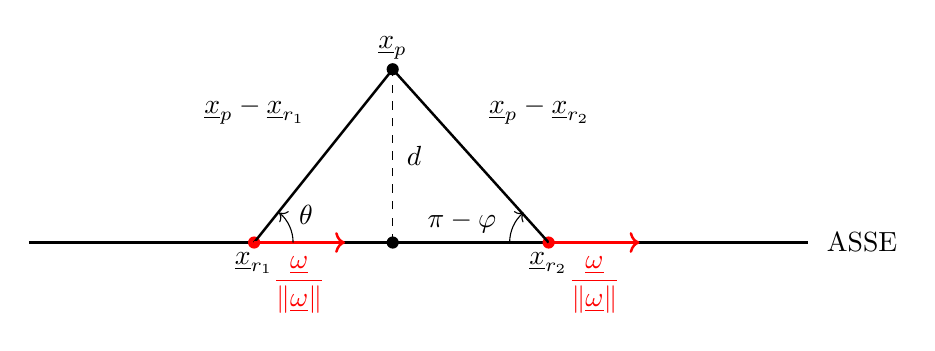
\begin{tikzpicture}[scale=1.1]
    % asse
    \draw[line width=0.9pt] (-4.2,0) -- (4.8,0);
    \node[right] at (4.9,0) {ASSE};

    % punti sull'asse
    \coordinate (R1) at (-1.6,0);
    \coordinate (R2) at (1.8,0);
    \coordinate (M) at (0,0);
    \coordinate (P) at (0,2.0);

    \fill[red] (R1) circle (2pt);
    \fill[red] (R2) circle (2pt);
    \fill (M) circle (2pt);
    \fill (P) circle (2pt);

    % segmenti
    \draw[line width=0.9pt] (R1) -- (P);
    \draw[line width=0.9pt] (R2) -- (P);
    \draw[dashed] (M) -- (P);

    % etichette punti
    \node[below] at (R1) {$\underline{x}_{r_1}$};
    \node[below] at (R2) {$\underline{x}_{r_2}$};
    \node[above] at (P) {$\underline{x}_p$};

    % etichette segmenti
    \node[above left] at (-0.9,1.25) {$\underline{x}_p-\underline{x}_{r_1}$};
    \node[above right] at (1.0,1.25) {$\underline{x}_p-\underline{x}_{r_2}$};

    % distanza d
    \node[right] at (0.05,1.0) {$d$};

    % frecce w/|w|
    \draw[red,->,line width=0.9pt] (-1.6,0) -- (-0.55,0);
    \draw[red,->,line width=0.9pt] (1.8,0) -- (2.85,0);
    \node[red,below] at (-1.08,-0.05) {$\dfrac{\underline{\omega}}{\|\underline{\omega}\|}$};
    \node[red,below] at (2.33,-0.05) {$\dfrac{\underline{\omega}}{\|\underline{\omega}\|}$};

    % angoli
    \draw[->] (-1.15,0) arc[start angle=0,end angle=50,radius=0.45];
    \node at (-1.0,0.32) {$\theta$};

    \draw[->] (1.35,0) arc[start angle=180,end angle=130,radius=0.45];
    \node at (0.8,0.24) {$\pi - \varphi$};
\end{tikzpicture}
\end{center}

Infatti, calcolando la differenza tra i due termini si ottiene:
\[
\underline{\omega}\wedge(\underline{x}_p-\underline{x}_{r_1}) - \underline{\omega}\wedge(\underline{x}_p-\underline{x}_{r_2}) = \underline{\omega}\wedge(\underline{x}_{r_2}-\underline{x}_{r_1}) = \underline{0}
\]
poiché $\underline{x}_{r_1}$ e $\underline{x}_{r_2}$ appartengono allo stesso asse, il vettore $(\underline{x}_{r_2}-\underline{x}_{r_1})$ è parallelo a $\underline{\omega}$. Di conseguenza, i due prodotti vettoriali sono identici.
\end{oss}


\begin{oss}{}
    Possiamo ricavare i punti dell'asse in forma parametrica tramite
\[
\underline{\omega}\wedge \underline{x}_r
=
-\underline{v}_q^{\perp}+\underline{\omega}\wedge \underline{x}_q
\qquad \Rightarrow \qquad
\underline{x}_r
=
t\,\underline{\omega}
-
\frac{\underline{\omega}\wedge\left(-\underline{v}_q^{\perp}+\underline{\omega}\wedge \underline{x}_q\right)}{\|\underline{\omega}\|^2},
\qquad t\in\mathbb{R}.
\]

Oppure in forma cartesiana utilizzando il fatto che
\[
\underline{v}_r \parallel \underline{\omega}
\qquad \forall\,\underline{x}_r
\text{ appartenente all'asse}
\]
tramite
\[
\frac{v_r^x}{\omega_x}
=
\frac{v_r^y}{\omega_y}
=
\frac{v_r^z}{\omega_z}.
\]

Dove $v_r^x$, $v_r^y$, $v_r^z$ devono essere espresse in funzione di
$x_r$, $y_r$, $z_r$, ad esempio utilizzando la formula fondamentale della cinematica.
\end{oss}

\begin{oss}{}
Nel caso di moti piani
\[
\underline{\omega}=(0,0,\omega_z)
\]
l'asse di Mozzi è ortogonale al piano del moto e ha un punto sul piano del moto. Intorno a questo punto $\bar{q}$, detto centro di istantanea rotazione, il moto è istantaneamente solo rotazionale:
\[
\underline{v}_p=\underline{\omega}\wedge(\underline{x}_p-\underline{x}_{\bar{q}}).
\]
Questo infatti è soggetto al vincolo $z_{\overline{q}} = 0 \Rightarrow \underline{v}_{\overline{q}} = 0$ essendo tutta la velocità di $\overline{q}$ diretta lungo l'asse $z$.
\end{oss}
\begin{example}{}
    Vogliamo studiare la posizione dell'asse di Mozzi di una trottola. Supponiamo che
la trottola sia a regime e che quindi abbia velocità angolare perpendicolare
al piano. Possiamo quindi studiare il moto come moto piano e cercare il centro
di istantanea rotazione.

\begin{figure}
\centering
\begin{minipage}{0.34\textwidth}
\centering
\begin{tikzpicture}[scale=1.2]
  % assi
  \draw[->] (0,0) -- (2.2,0) node[right] {$u$};
  \draw[->] (0,0) -- (0,2.2) node[above] {$z$};
  \draw[->] (0,0) -- (-1.3,-1.3) node[below] {$x$};

  % trottola
  \draw (-0.5,0.95) .. controls (-0.25,1.15) and (0.25,1.15) .. (0.5,0.95);
  \draw (-0.5,0.95) .. controls (-0.2,0.72) and (0.2,0.72) .. (0.5,0.95);
  \draw (-0.5,0.95) -- (-0.2,0.25);
  \draw (0.5,0.95) -- (0.2,0.25);
  \draw (-0.2,0.25) -- (0.2,0.25);
  \draw (-0.2,0.25) -- (0,-0.45);
  \draw (0.2,0.25) -- (0,-0.45);
  \fill (0,-0.45) circle (1.2pt);
  \node[below right] at (0,-0.45) {$c$};

  % omega
  \draw[red,->,line width=0.9pt] (0.25,1.05) -- (0.25,2.0);
  \node[red,right] at (0.25,1.65) {$\omega$};
\end{tikzpicture}
\end{minipage}
\hfill
\begin{minipage}{0.48\textwidth}
\centering
\begin{tikzpicture}[scale=1.2]
  % assi
  \draw[->] (-0.2,0) -- (3.2,0) node[right] {$x$};
  \draw[->] (0,-1.2) -- (0,2.2) node[above] {$u$};

  % disco
  \draw (1.45,1.25) circle (0.65);
  \fill (1.45,1.25) circle (1.1pt);
  \node[below right] at (1.45,1.25) {$c$};

  % velocità
  \draw[->,line width=0.9pt] (1.45,1.25) -- (1.1,1.72);
  \node[above left] at (1.23,1.55) {$\underline{v}_c$};

  % omega
  \draw[red,->,line width=0.9pt] (2.02,2.02) arc[start angle=20,end angle=160,radius=0.63];
  \node[red] at (1.45,2.25) {$\omega$};
\end{tikzpicture}
\end{minipage}
\end{figure}

Sia $\underline{x}_I$ il centro di istantanea rotazione. Sappiamo che
$\underline{v}_I=\underline{v}_p^{\parallel}=0 \ \forall p$. Allora
\[
0=\underline{v}_c+\omega\wedge(\underline{x}_I-\underline{x}_c)
\]
\[
\Rightarrow\quad
0=\hat{k}\wedge \underline{v}_c+\hat{k}\wedge\bigl(\omega\wedge(\underline{x}_I-\underline{x}_c)\bigr)
\]
\[
\Rightarrow\quad
0=\hat{k}\wedge \underline{v}_c+\omega\cdot \|\underline{x}_I-\underline{x}_c\|\cdot
\hat{k}\wedge\left(\hat{k}\wedge
\frac{\underline{x}_I-\underline{x}_c}{\|\underline{x}_I-\underline{x}_c\|}\right)
\]
ora dal momento che $ \frac{\underline{x}_I-\underline{x}_c}{\|\underline{x}_I-\underline{x}_c\|}$ ha coordinata lungo $\hat k$ nulla risulta che
\[
\Rightarrow\quad
0=\hat{k}\wedge \underline{v}_c-\omega\cdot \|\underline{x}_I-\underline{x}_c\|\cdot
\frac{\underline{x}_I-\underline{x}_c}{\|\underline{x}_I-\underline{x}_c\|}
=
\hat{k}\wedge \underline{v}_c-\omega\cdot(\underline{x}_I-\underline{x}_c)
\]
\[
\Rightarrow\quad
\underline{x}_I-\underline{x}_c=\frac{\hat{k}\wedge \underline{v}_c}{\omega}
\qquad \Rightarrow \qquad
\underline{x}_I=\underline{x}_c+\frac{\hat{k}\wedge \underline{v}_c}{\omega}.
\]

Abbiamo quindi ottenuto che $\underline{x}_I$ sta sulla retta perpendicolare a
$\underline{v}_c$ e passante per $\underline{x}_c$. Il verso dipende dal segno di $\omega$.

\begin{figure}
\centering
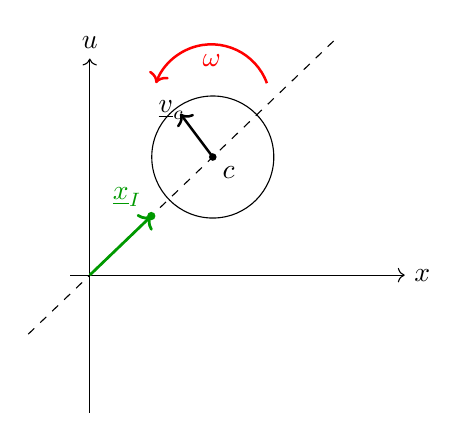
\begin{tikzpicture}[scale=1.25]
  % assi
  \draw[->] (-0.2,0) -- (3.2,0) node[right] {$x$};
  \draw[->] (0,-1.4) -- (0,2.2) node[above] {$u$};

  % retta tratteggiata
  \draw[dashed] (-0.625 , -0.6) -- (2.5,2.4);

  % disco
  \draw (1.25,1.2) circle (0.62);
  \fill (1.25,1.2) circle (1.1pt);
  \node[below right] at (1.25,1.2) {$c$};

  % velocità
  \draw[->,line width=0.9pt] (1.25,1.2) -- (0.92,1.64);
  \node[above left] at (1.06,1.48) {$\underline{v}_c$};

  % omega
  \draw[red,->,line width=0.9pt] (1.8,1.95) arc[start angle=20,end angle=160,radius=0.6];
  \node[red] at (1.24,2.18) {$\omega$};

  % x_I
  \coordinate (XI) at (0.625,0.6);
  \draw[green!60!black,->,line width=1pt] (0,0) -- (XI);
  \fill[green!60!black] (XI) circle (1.2pt);
  \node[green!60!black,above left] at (XI) {$\underline{x}_I$};
\end{tikzpicture}
\end{figure}

Più nello specifico la distanza dal centro $c$ vale
\[
\|\underline{x}_I-\underline{x}_c\|
=
\left\|\frac{\hat{k}\wedge \underline{v}_c}{\omega}\right\|
=
\frac{\|\hat{k}\wedge \underline{v}_c\|}{|\omega|}
=
\frac{\|\underline{v}_c\|}{|\omega|}
\qquad
(\hat{k}\perp \underline{v}_c).
\]

E quindi nel caso in cui $\underline{v}_c=0$ l'asse di Mozzi coincide con
l'asse verticale di simmetria della trottola.

In generale il centro di istantanea rotazione può essere un punto interno
alla trottola, sul bordo o esterno.
\end{example}
\begin{examplebreak}{}
    Troviamo il centro di istantanea rotazione del sistema caratterizzato dai vincoli $x_A = y_B = 0$ che ha quindi un solo grado di libertà.
\begin{center}
\begin{tikzpicture}[scale=1.15]
    % assi
    \draw[->] (-0.6,0) -- (5.2,0);
    \draw[->] (0,-0.6) -- (0,3.6);

    % punti
    \coordinate (A) at (0,2.7);
    \coordinate (B) at (4.0,0);
    \coordinate (Q) at (4.0,2.7);

    % asta
    \draw[line width=0.9pt] (A) -- (B);
    \node at (2.15,1.65) {$\ell$};

    % tratteggi
    \draw[dashed] (A) -- (Q);
    \draw[dashed] (B) -- (Q);

    % punti marcati
    \fill (A) circle (1.8pt);
    \fill (B) circle (1.8pt);
    \fill (Q) circle (1.8pt);

    % etichette
    \node[left] at (A) {$\underline{x}_A$};
    \node[below] at (B) {$\underline{x}_B$};
    \node[above] at (Q) {$\underline{x}_q$};

    % velocità
    \draw[->,red,line width=0.9pt] (A) -- ++(0,-1.0);
    \node[red,left] at (-0.05,1.75) {$\underline{v}_A$};

    \draw[->,red,line width=0.9pt] (B) -- ++(1.0,0);
    \node[red,above] at (4.55,0.05) {$\underline{v}_B$};
\end{tikzpicture}
\end{center}



\[
\underline{v}_A=\underline{\omega}\wedge(\underline{x}_A-\underline{x}_q)
\qquad\Rightarrow\qquad
\underline{x}_A-\underline{x}_q \text{ è parallelo a } \hat{\imath}
\]

\[
\underline{v}_B=\underline{\omega}\wedge(\underline{x}_B-\underline{x}_q)
\qquad\Rightarrow\qquad
\underline{x}_B-\underline{x}_q \text{ è parallelo a } \hat{\jmath}
\]

In particolare
\[
\underline{x}_A-\underline{x}_q\in \operatorname{span}\{\hat{\imath}\}
\qquad\text{e}\qquad
\underline{x}_B-\underline{x}_q\in \operatorname{span}\{\hat{\jmath}\}.
\]

Ovvero
\[
\underline{x}_q\in \underline{x}_A+\operatorname{span}\{\hat{\imath}\},
\qquad
\underline{x}_q\in \underline{x}_B+\operatorname{span}\{\hat{\jmath}\},
\]
ovvero
\[
\underline{x}_q\in
\bigl(\underline{x}_A+\operatorname{span}\{\hat{\imath}\}\bigr)
\cap
\bigl(\underline{x}_B+\operatorname{span}\{\hat{\jmath}\}\bigr).
\]

Ma dal momento che
\[
\operatorname{span}\{\hat{\jmath}\}\cap \operatorname{span}\{\hat{\imath}\}=\{0\},
\]
$\underline{x}_q$ è l'unico vettore nell'intersezione dei due affini e può essere individuato geometricamente come in figura o analiticamente dai vincoli
\[
y=y_A
\qquad\text{e}\qquad
x=x_B.
\]
\end{examplebreak}

\chapter{Dinamica del corpo rigido}
Consideriamo un punto materiale con posizione
\[
\underline{x}(t)=\bigl(x(t),y(t),z(t)\bigr).
\]

Per avere una forma analitica di $\underline{x}(t)$ dobbiamo passare dalla legge di Newton
\[
m\,\ddot{\underline{x}}=\underline{f}\bigl(\underline{x},\dot{\underline{x}},t\bigr),
\]
Dato un corpo dotato di massa inerziale $m$ quest'ultima è quindi la costante di proporzionalità tra accelerazione e risultante delle forze.

\begin{oss}{}
$\underline{f}$ non dipende mai da $\ddot{\underline{x}}$. Questa è un'evidenza fisica.
\end{oss}

Consideriamo un insieme di $n$ punti materiali. Per ogni punto possiamo scrivere
\[
m_i\,\ddot{\underline{x}}_i=\underline{f}_i\bigl(x_1,\dots,x_n,\dot{x}_1,\dots,\dot{x}_n,t\bigr).
\]

\begin{oss}{}
Nelle $\{\underline{f}_i\}$ sono comprese anche le forze vincolari, che pur non essendo funzioni esplicite di
\[
(x_1,\dots,x_n,\dot{x}_1,\dots,\dot{x}_n,t),
\]
ne dipendono comunque in maniera implicita.
\end{oss}\begin{example}{}
Consideriamo un sistema di $3$ punti materiali vincolati attraverso due aste rigide di lunghezza $d_1,d_2$ e due molle di rigidezza $K_1,K_2$, disposti come in figura.

\begin{figure}
\centering
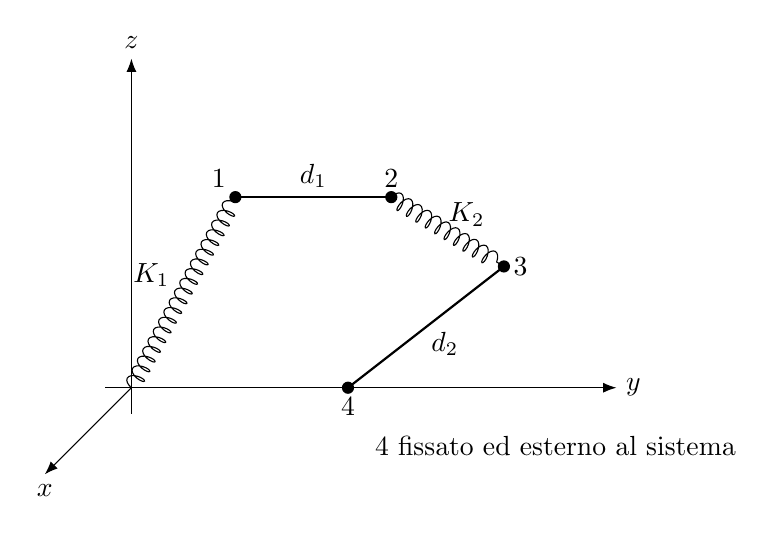
\begin{tikzpicture}[scale=1.1, >=Latex]

% assi
\draw[->] (-0.3,0) -- (5.6,0) node[right] {$y$};
\draw[->] (0,-0.3) -- (0,3.8) node[above] {$z$};
\draw[->] (0,0) -- (-1.0,-1.0) node[below] {$x$};

% punti
\coordinate (O) at (0,0);
\coordinate (P1) at (1.2,2.2);
\coordinate (P2) at (3.0,2.2);
\coordinate (P3) at (4.3,1.4);
\coordinate (P4) at (2.5,0);

% punti materiali
\fill (P1) circle (2pt) node[above left] {$1$};
\fill (P2) circle (2pt) node[above] {$2$};
\fill (P3) circle (2pt) node[right] {$3$};
\fill (P4) circle (2pt) node[below] {$4$};

% molla K1 tra O e P1
\draw[decorate, decoration={coil, aspect=0.45, segment length=4pt, amplitude=3pt}]
  (O) -- (P1);
\node[left] at (0.55,1.3) {$K_1$};

% asta rigida d1 tra P1 e P2
\draw[thick] (P1) -- (P2);
\node[above] at (2.1,2.2) {$d_1$};

% molla K2 tra P2 e P3
\draw[decorate, decoration={coil, aspect=0.45, segment length=4pt, amplitude=3pt}]
  (P2) -- (P3);
\node[right] at (3.55,2.0) {$K_2$};

% asta rigida d2 tra P4 e P3
\draw[thick] (P4) -- (P3);
\node[below right] at (3.35,0.75) {$d_2$};


% nota punto 4
\node[below right] at (2.7,-0.45) {$4$ fissato ed esterno al sistema};

\end{tikzpicture}
\end{figure}

Imponiamo il vincolo olonomo
\[
\lvert \underline{x}_1-\underline{x}_2\rvert=d_1=\text{cost}.
\]
Come tutti i vincoli olonomi, esso comporta una reazione vincolare, cioè una forza incognita che permette il soddisfacimento del vincolo.

Allo stesso modo imponiamo
\[
\lvert \underline{x}_3-\underline{x}_4\rvert=d_2=\text{cost}.
\]

Detta $\underline{f}_i$ la risultante delle forze agenti sul punto $i$-esimo, abbiamo
\[
\underline{f}_1=-K_1(\underline{x}_1-\underline{0})+\underline{f}_{12},
\]
dove $-K_1(\underline{x}_1-\underline{0})$ è una forza attiva esterna, mentre $\underline{f}_{12}$ è una forza interna vincolare.

Inoltre
\[
\underline{f}_2=\underline{f}_{21}-K_2(\underline{x}_2-\underline{x}_3),
\]
dove $\underline{f}_{21}$ è una forza interna vincolare, mentre $-K_2(\underline{x}_2-\underline{x}_3)$ è una forza attiva interna.

Infine
\[
\underline{f}_3=-K_2(\underline{x}_3-\underline{x}_2)+\underline{f}_{34},
\]
dove $-K_2(\underline{x}_3-\underline{x}_2)$ è una forza attiva interna, mentre $\underline{f}_{34}$ è una forza esterna vincolare.

Notiamo che
\[
\underline{f}_{23}=-K_2(\underline{x}_2-\underline{x}_3)
              =K_2(\underline{x}_3-\underline{x}_2)
              =-\underline{f}_{32},
\]
quindi tali forze soddisfano il principio di azione e reazione.
\end{example}

\begin{example}{}
Descriviamo la dinamica di un moto piano di un punto. Imponiamo il vincolo
\[
z_P=0.
\]

\begin{figure}
\centering
\begin{tikzpicture}[scale=1.1, >=Latex]
  % piano vincolante
  \draw (-2.2,0) -- (3.2,0);
  \draw (-1.0,1.6) -- (3.2,1.6);
  \draw (-2.2,0) -- (-1.0,1.6);

  % punto P
  \fill (0.2,0.8) circle (2pt) node[right] {$P$};

  % asse verticale delle forze
  \draw[->] (0.2,0.8) -- (0.2,2.0);
  \node[right] at (0.2,1.85) {$\underline{R}$};

  \draw[->] (0.2,0.8) -- (0.2,-0.4);
  \node[right] at (0.2,-0.25) {$m\underline{g}$};
\end{tikzpicture}
\end{figure}

Se
\[
m\,\ddot{\underline{x}}_P=0,
\]
allora c'è una forza esterna vincolare $\underline{R}$ dovuta al vincolo $z_P=0$ che annulla $m\underline{g}$, ovvero
\[
\underline{R}=m\underline{g}.
\]
\end{example}

\section{Prima equazione cardinale del moto di un corpo rigido}
Consideriamo un sistema di $n$ particelle caratterizzate ognuna da una posizione $\underline{x}_i$ e da una massa $m_i$.

\begin{definition}{}
Si dice centro di massa del sistema
\[
\underline{x}_G = \frac{\sum_{i=1}^{n} m_i \,\underline{x}_i}{\sum_{i=1}^{n} m_i}.
\]
\end{definition}

\begin{definition}{}
Si dice vettore posizione del punto $i$-esimo rispetto al centro di massa
\[
\underline{x}_i' = \underline{x}_i - \underline{x}_G.
\]
\end{definition}

\begin{figure}[H]
\centering
\begin{tikzpicture}[scale=1.2, >=Latex]

% assi 3D
\draw[->] (-1.0,0,0) -- (3.0,0,0) node[right] {$x$};
\draw[->] (0,-1.0,0) -- (0,3.0,0) node[above] {$y$};
\draw[->] (0,0,-1.0) -- (0,0,3.0) node[above] {$z$};

% punti e vettori
\coordinate (O) at (0,0,0); % origine
\coordinate (X1) at (2,2,1);  % primo punto
\coordinate (X2) at (1.5,3,2); % secondo punto

% vettori
\draw[->,red] (O) -- (X1) node[midway, below right] {$\underline{x}_i$}; % vettore x1
\draw[->,blue] (O) -- (X2) node[midway, above right] {$\underline{x}_G$}; % vettore x2

% vettore differenza
\draw[->,green] (X2) -- (X1) node[midway, above right] {$\underline{x}_i'$}; % differenza tra i vettori

\end{tikzpicture}
\end{figure}

\begin{oss}{}
\[
\sum_{i=1}^{n} m_i \,\underline{x}_i' = \sum_{i=1}^{n} m_i \,(\underline{x}_i - \underline{x}_G) = \sum_{i=1}^{n} m_i \, \underline{x}_i - \sum_{i=1}^{n} m_i \,\underline{x}_G
\]
\[
\underline{x}_G'
=
\frac{\sum_{i=1}^{n} m_i \underline{x}_i'}{\sum_{i=1}^{n} m_i}
=
\frac{\sum_{i=1}^{n} m_i(\underline{x}_i-\underline{x}_G)}{\sum_{i=1}^{n} m_i}
\]
\[
=
\frac{\sum_{i=1}^{n} m_i \underline{x}_i}{\sum_{i=1}^{n} m_i}
-
\frac{\sum_{i=1}^{n} m_i \underline{x}_G}{\sum_{i=1}^{n} m_i}
=
\underline{x}_G-\underline{x}_G
=
\underline{0}
\]

Questo è ovvio perché la posizione del centro di massa calcolato in un sistema di riferimento che ha l'origine nel centro di massa è l'origine stessa.
\end{oss}

Consideriamo il sistema di $n$ punti materiali di posizioni $\underline{x}_i$ e masse $m_i$ sottoposti a forze di risultante $\underline{f}_i$. Allora per ogni punto vale:
\[
m_i \underline{\ddot{x}}_i = \underline{f}_i.
\]
Sommiamo su tutti i punti:
\[
\sum_{i=1}^{n} m_i \underline{\ddot{x}}_i = \sum_{i=1}^{n} m_i \frac{d^2}{dt^2} \left( \underline{x}_G + \underline{x}_i' \right) = \frac{d^2}{dt^2} \left( \sum_{i=1}^{n} m_i \underline{x}_G + \sum_{i=1}^{n} m_i \underline{x}_i' \right)
\]

\[
= m \frac{d^2}{dt^2} \underline{x}_G = \frac{d}{dt} \left( m \underline{v}_G \right)
\]

Ora, dette $\underline{f}_i^{\text{est}}$ e $\underline{f}_i^{\text{int}}$ rispettivamente la risultante delle forze esterne che agiscono su $i$ e la risultante delle forze interne che agiscono su $i$, possiamo scrivere:
\[
\underline{f}_i = \underline{f}_i^{\text{est}} + \underline{f}_i^{\text{int}} = \underline{f}_i^{\text{est}} + \sum_{\substack{j=1 \\ j \neq i}}^{n} \underline{f}_{ij}
\]
Allora otteniamo
\[
\sum_{i=1}^{n} m_i \underline{\ddot{x}}_i = \sum_{i=1}^{n} \underline{f}_i = \sum_{i=1}^{n} \underline{f}_i^{\text{est}} + \sum_{i=1}^{n} \sum_{\substack{j=1 \\ j \neq i}}^{n} \underline{f}_{ij} = \sum_{i=1}^{n} \underline{f}_i^{\text{est}}
\]
Dal momento che $\sum_{i=1}^{n} \sum_{\substack{j=1 \\ j \neq i}}^{n} \underline{f}_{ij} = \underline{0}$ per il principio di azione e reazione (le forze interne si annullano a due a due!).\\
Otteniamo infine
\[
\frac{d}{dt} \left( m \underline{v}_G \right) = \sum_{i=1}^{n} \underline{f}_i^{\text{est}}.
\]
detta \textbf{prima equazione cardinale del moto di un corpo rigido.}

\begin{oss}{}
Il centro di massa di un corpo rigido si comporta come un punto materiale sottoposto solo alle forze esterne.
\end{oss}


\begin{example}{}
    Considero un disco piano che si muove di moto di puro strisciamento con il suo centro vincolato ad una molla orizzontale.

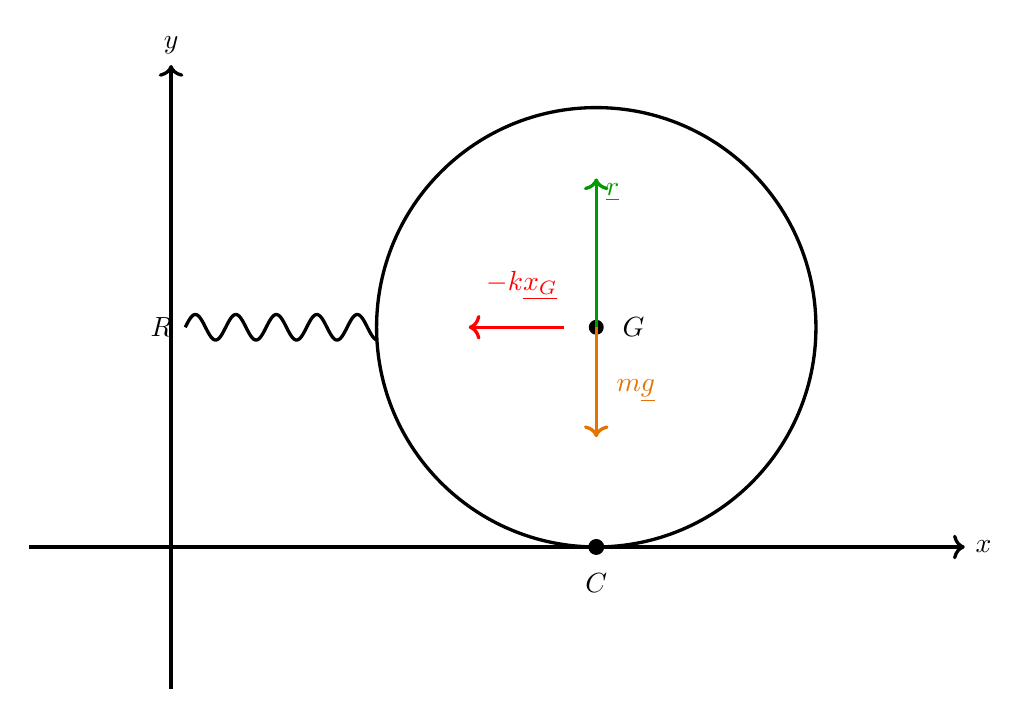
\begin{tikzpicture}[scale=0.9]
  % assi
  \draw[very thick, ->] (-2,0) -- (11.2,0) node[right] {$x$};
  \draw[very thick, ->] (0,-2) -- (0,6.8) node[above] {$y$};

  % disco
  \draw[very thick] (6,3.1) circle (3.1);

  % punto di contatto C
  \fill (6,0) circle (3.2pt);
  \node[below=6pt] at (6,0) {$C$};

  % centro G
  \fill (6,3.1) circle (3pt);
  \node[right=6pt] at (6,3.1) {$G$};

  % molla orizzontale verso l'asse y
  \draw[very thick]
    plot[smooth, samples=200, domain=0:2.7]
    ({0.2+\x},{3.1 + 0.18*sin(deg(11*\x))});
  \node[left] at (0.15,3.1) {$R$};

  % forza elastica
  \draw[red, very thick, ->] (5.55,3.1) -- (4.2,3.1);
  \node[red, above] at (4.95,3.35) {$-k\underline{x_G}$};

  % reazione vincolare r
  \draw[green!60!black, very thick, ->] (6,3.1) -- (6,5.2);
  \node[green!60!black, right] at (6,5.0) {$\underline{r}$};

  % peso mg
  \draw[orange!90!black, very thick, ->] (6,3.1) -- (6,1.55);
  \node[orange!90!black, right] at (6.15,2.2) {$m\underline{g}$};
\end{tikzpicture}

I vincoli sono quindi
\[
\dot{x}_C = 0 \quad x_C = x_G
\]
che portano il sistema ad un grado di libertà. Ai vincoli è associata una forza vincolare $\underline{r}$, inoltre possiamo far confluire tutta la massa nel centro di massa e applicare lì la forza peso
\[
m\underline{g} = \sum_{i=1}^m m_i \underline{g}.
\]
Abbiamo quindi
\[
m \underline{\ddot{x}_G} = -k \underline{x_G} + \underline{r} + m\underline{g}
\]
e dal momento che
\[
\underline{\ddot{x}_G} = \ddot{x}_G \hat{i} \quad \text{e} \quad -k \underline{x_G}= -k x_G \hat{i}
\]
allora necessariamente
\[
\underline{r} = -m\underline{g}.
\]
\end{example}

\begin{oss}{}
In generale non è possibile disaccoppiare traslazione del centro di massa e rotazione.

\begin{center}
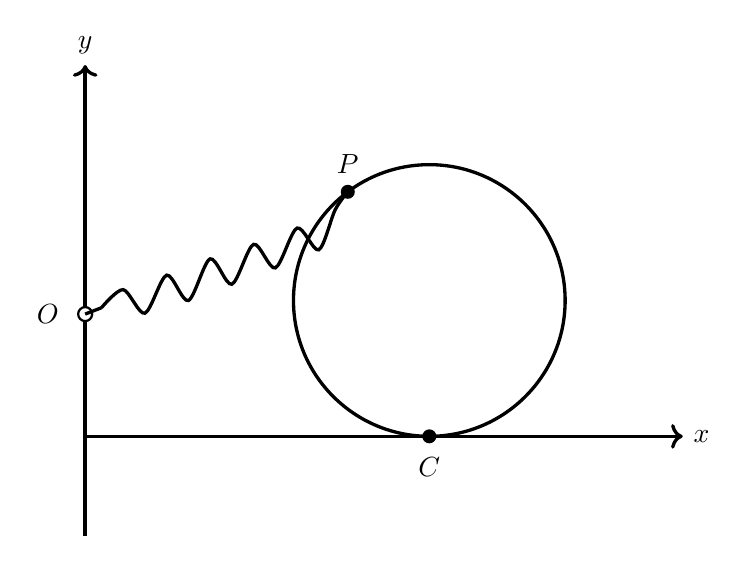
\begin{tikzpicture}[scale=1.15]
  % assi
  \draw[very thick,->] (0,-1.1) -- (0,4.1) node[above] {$y$};
  \draw[very thick,->] (0,0) -- (6.6,0) node[right] {$x$};

  % disco
  \def\R{1.5}
  \coordinate (G) at (3.8,1.5);
  \coordinate (C) at (3.8,0);
  \coordinate (O) at (0,1.35);
  \coordinate (P) at (2.9,2.7);

  \draw[very thick] (G) circle (\R);

  % punti
  \filldraw[fill=white,draw=black,line width=0.8pt] (O) circle (2.2pt);
  \node[left=6pt] at (O) {$O$};

  \fill (P) circle (2.2pt);
  \node[above=3pt] at (P) {$P$};

  \fill (C) circle (2.2pt);
  \node[below=4pt] at (C) {$C$};

  % molla
  \draw[very thick]
    (O) -- (0.18,1.42)
    plot[smooth] coordinates {
      (0.18,1.42) (0.42,1.62) (0.66,1.36) (0.90,1.78)
      (1.14,1.50) (1.38,1.96) (1.62,1.68) (1.86,2.12)
      (2.10,1.86) (2.34,2.30) (2.58,2.06) (2.76,2.50)
      (2.90,2.70)
    };
\end{tikzpicture}
\end{center}

Rilassando il moto di puro strisciamento imponendo solo
\[
y_C^{\text{Disco}}=0
\]
istantaneamente e considerando il caso in cui la molla non è orizzontale si ottiene
\[
m\ddot{\underline{x}}_G=\underline{f}^{\mathrm{ext}}=-k\bigl(\underline{x}_P-\underline{x}_O\bigr)
\]
che dipende da \(\underline{\omega}\) dal momento che \(\underline{x}_P\) dipende da \(\underline{\omega}\) attraverso
\[
\underline{v}_P=\underline{v}_C+\underline{\omega}\wedge\bigl(\underline{x}_P-\underline{x}_C\bigr).
\]
\end{oss}


\begin{example}{}
Consideriamo un sistema costituito da una persona su una barca e dalla barca. Supponiamo inizialmente che sia la barca che la persona siano fermi rispetto ad un sistema di riferimento fisso posto sulla superficie dell'acqua. Inoltre sul sistema non agisce una risultante non nulla di forze esterne.

\begin{center}
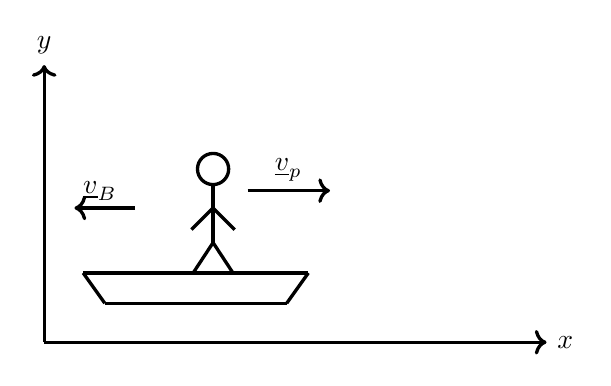
\begin{tikzpicture}[scale=1.1]
  % assi
  \draw[very thick,->] (0,0) -- (5.8,0) node[right] {$x$};
  \draw[very thick,->] (0,0) -- (0,3.2) node[above] {$y$};

  % barca
  \draw[very thick] (0.45,0.8) -- (3.05,0.8);
  \draw[very thick] (0.70,0.45) -- (2.80,0.45);
  \draw[very thick] (0.45,0.8) -- (0.70,0.45);
  \draw[very thick] (3.05,0.8) -- (2.80,0.45);

  % omino
  \draw[very thick] (1.95,2.0) circle (0.18);
  \draw[very thick] (1.95,1.82) -- (1.95,1.15);
  \draw[very thick] (1.95,1.55) -- (1.70,1.30);
  \draw[very thick] (1.95,1.55) -- (2.20,1.30);
  \draw[very thick] (1.95,1.15) -- (1.72,0.80);
  \draw[very thick] (1.95,1.15) -- (2.18,0.80);

  % velocità
  \draw[very thick,->] (2.35,1.75) -- (3.30,1.75);
  \node[above] at (2.82,1.75) {$\underline{v}_p$};

  \draw[very thick,->] (1.05,1.55) -- (0.35,1.55);
  \node[left] at (0.95,1.75) {$\underline{v}_B$};
\end{tikzpicture}
\end{center}

Si ha quindi
\[
\underline{f}^{\mathrm{est}}
=
\frac{d}{dt}\,m\underline{v}_G
=
\frac{d}{dt}\left(m_p\underline{v}_p + m_B\underline{v}_B\right)
=
\underline{0}.
\]

Quindi
\[
\left\{
\begin{aligned}
m_p \frac{dv_{p,x}}{dt} &= -m_B \frac{dv_{B,x}}{dt},\\
m_p \frac{dv_{p,y}}{dt} &= -m_B \frac{dv_{B,y}}{dt},
\end{aligned}
\right.
\qquad\Longrightarrow\qquad
\left\{
\begin{aligned}
m_p v_{p,x} &= -m_B v_{B,x} + C_1,\\
m_p v_{p,y} &= -m_B v_{B,y} + C_2.
\end{aligned}
\right.
\]

E imponendo
\[
\underline{v}_B = \underline{v}_p = \underline{0}
\]
si ottiene \(C_1 = C_2 = 0\), ovvero
\[
\underline{v}_p = -\frac{m_B}{m_p}\,\underline{v}_B.
\]
\end{example}



\section{Seconda equazione cardinale del moto di un corpo rigido}


Vogliamo ora introdurre la dinamica rotazionale. Partiamo dal caso più semplice. Consideriamo un punto materiale dotato della quantità di moto \(m\underline{v}\), possiamo scrivere la legge di Newton nella forma
\[
\frac{d}{dt}(m\underline{v}) = \underline{f}(\underline{x}, \underline{v}, t)
\]
A partire da quest'ultima  dimostriamo che, definito \( \underline{x} \wedge \underline{f}(\underline{x}, \underline{v}, t) \) il momento della risultante delle forze rispetto all'origine vale
\[
\frac{d}{dt}(\underline{x} \wedge m\underline{v}) = \underline{x} \wedge \underline{f}(\underline{x}, \underline{v}, t),
\]
dove \( \underline{x} \wedge m\underline{v} \) è detto momento della quantità di moto rispetto all'origine o momento angolare rispetto all'origine. Infatti
\[
\frac{d}{dt} (\underline{x} \wedge m \underline{v}) = \underline{v} \wedge m\underline{v} + \underline{x} \wedge \frac{d}{dt}(m\underline{v}) = \underline{v} \wedge m\underline{v} + \underline{x} \wedge \underline{f} = \underline{x} \wedge \underline{f}.
\]
Se \( \underline{x}_0 \) è un punto fisso si dimostra in modo analogo che
\[
\frac{d}{dt} \left( (\underline{x} - \underline{x}_0) \wedge m\underline{v} \right) = (\underline{x} - \underline{x}_0) \wedge \underline{f}.
\]

Infine, se \( \underline{x}_0(t) \) non è fisso vale
\[
\frac{d}{dt} \left( (\underline{x}(t) - \underline{x}_0(t)) \wedge m\underline{v} \right) = (\underline{x}(t) - \underline{x}_0(t)) \wedge \underline{f} - \underline{v}_0 \wedge m\underline{v}.
\]
Infatti
\[
\frac{d}{dt}
\left[
(\underline{x}(t)-\underline{x}_0(t))\wedge m\underline{v}
\right]
=
\frac{d}{dt}
(\underline{x}(t)-\underline{x}_0(t))
\wedge m\underline{v}
+
(\underline{x}(t)-\underline{x}_0(t))
\wedge
\frac{d}{dt}(m\underline{v})
\]
\[
=
(\underline{v}-\underline{v}_0)\wedge m\underline{v}
+
(\underline{x}(t)-\underline{x}_0(t))\wedge \underline{f}
\]
\[
=
\underline{v}\wedge m\underline{v}
-
\underline{v}_0\wedge m\underline{v}
+
(\underline{x}(t)-\underline{x}_0(t))\wedge \underline{f}
\]
\[
=
(\underline{x}(t)-\underline{x}_0(t))\wedge \underline{f}
-
\underline{v}_0\wedge m\underline{v}
\]

Dimostriamo il seguente lemma di calcolo vettoriale che ci servirà nel seguito.
\begin{lemma}{}
Siano \( \underline{a}, \underline{b}, \underline{c} \in \mathbb{R}^3 \). Allora
\[
\underline{a} \wedge (\underline{b} \wedge \underline{c}) = \underline{b} (\underline{a} \cdot \underline{c}) - \underline{c} (\underline{b} \cdot \underline{a}).
\]
\end{lemma}
\inizioapprof
\begin{proof}
Siano \(\underline{a}=(a_1,a_2,a_3)\), \(\underline{b}=(b_1,b_2,b_3)\), \(\underline{c}=(c_1,c_2,c_3)\).

\[
\underline{b}\wedge \underline{c}=
\left|
\begin{array}{ccc}
\hat{\imath} & \hat{\jmath} & \hat{k}\\
b_1 & b_2 & b_3\\
c_1 & c_2 & c_3
\end{array}
\right|
=
\hat{\imath}(b_2c_3-b_3c_2)-\hat{\jmath}(b_1c_3-c_1b_3)+\hat{k}(b_1c_2-c_1b_2)
\]
\[
=
(b_2c_3-b_3c_2,\;c_1b_3-b_1c_3,\;b_1c_2-c_1b_2)
\]

\[
\Rightarrow\ \underline{a}\wedge(\underline{b}\wedge \underline{c})=
\left|
\begin{array}{ccc}
\hat{\imath} & \hat{\jmath} & \hat{k}\\
a_1 & a_2 & a_3\\
b_2c_3-b_3c_2 & c_1b_3-b_1c_3 & b_1c_2-c_1b_2
\end{array}
\right|
=
\]

\[
=
\hat{\imath}(a_2b_1c_2-a_2c_1b_2-a_3c_1b_3+a_3b_1c_3)
-\hat{\jmath}(a_1b_1c_2-a_1c_1b_2-a_3b_2c_3+a_3b_3c_2)+
\]
\[
+\hat{k}(a_1c_1b_3-a_1b_1c_3-a_2b_2c_3+a_2b_3c_2)=
\]

\[
=
(a_2b_1c_2-a_2c_1b_2-a_3c_1b_3+a_3b_1c_3,\;
a_1c_1b_2-a_1b_1c_2+a_3b_2c_3-a_3b_3c_2,\;
\]
\[
,a_1c_1b_3-a_1b_1c_3-a_2b_2c_3+a_2b_3c_2)=
\]

\[
=
\bigl(
b_1[a_2c_2+a_3c_3+a_1c_1]-c_1[a_1b_1+a_2b_2+a_3b_3],\;
b_2[a_1c_1+a_2c_2+a_3c_3]-c_2[a_1b_1+a_2b_2+a_3b_3],\;
\]
\[
,b_3[a_1c_1+a_2c_2+a_3c_3]-c_3[a_1b_1+a_2b_2+a_3b_3]
\bigr)=
\]

\[
=
(b_1\cdot \underline{a}\cdot \underline{c}-c_1\cdot \underline{a}\cdot \underline{b},\;
b_2\cdot \underline{a}\cdot \underline{c}-c_2\cdot \underline{a}\cdot \underline{b},\;
b_3\cdot \underline{a}\cdot \underline{c}-c_3\cdot \underline{a}\cdot \underline{b})
=
\underline{b}\cdot \underline{a}\cdot \underline{c}-\underline{c}\cdot \underline{a}\cdot \underline{b}
\]
\end{proof}
\fineapprof
Consideriamo un sistema di \(n\) particelle ognuna caratterizzata da posizione \(\underline{x}_i\), velocità \(\underline{v}_i\) e massa \(m_i\).

Per ogni particella scriviamo l'equazione del momento della quantità di moto per il punto \(i\)-esimo rispetto a \(O\).
\[
\frac{d}{dt}\left(\underline{x}_i\wedge m_i\,\underline{v}_i\right)=\underline{x}_i\wedge \underline{f}_i.
\]

Decompongo
\[
\underline{x}_i=\underline{x}_G+\underline{x}_i'
\quad\Rightarrow\quad
\underline{v}_i=\underline{v}_G+\underline{v}_i'
\]

\[
\Rightarrow\quad
\frac{d}{dt}\left((\underline{x}_G+\underline{x}_i')\wedge m_i(\underline{v}_G+\underline{v}_i')\right)
=
(\underline{x}_G+\underline{x}_i')\wedge \underline{f}_i
\]

Sommando per tutti i punti e usando la linearità della derivata si ottiene
\[
\frac{d}{dt}\sum_{i=1}^{n}(\underline{x}_G+\underline{x}_i')\wedge m_i(\underline{v}_G+\underline{v}_i')
=
\sum_{i=1}^{n}(\underline{x}_G+\underline{x}_i')\wedge \underline{f}_i
\]

Nel membro di destra evidenzio le forze interne ed esterne in \(\underline{f}_i\)

\[
\sum_{i=1}^{n}\underline{x}_i\wedge \underline{f}_i
=
\sum_{i=1}^{n}\underline{x}_i\wedge \underline{f}_i^{\mathrm{ext}}
+
\sum_{i=1}^{n}\underline{x}_i\wedge \sum_{\substack{j=1\\ i\neq j}}^{n}\underline{f}_{ij}
\overset{\textcolor{red}{(1)}}{=}
\sum_{i=1}^{n}\underline{x}_i\wedge \underline{f}_i^{\mathrm{ext}}
+
\]

\[
+\sum_{\{i,j\}}(\underline{x}_i-\underline{x}_j)\wedge \underline{f}_{ij}
\overset{\textcolor{red}{(2)}}{=}
\sum_{i=1}^{n}\underline{x}_i\wedge \underline{f}_i^{\mathrm{ext}}
\]

Dove in \(\textcolor{red}{(1)}\) abbiamo usato il principio di azione-reazione e in \(\textcolor{red}{(2)}\) il fatto che \(\underline{x}_i-\underline{x}_j \parallel \underline{f}_{ij}\).\\
Nel termine di sinistra
\[
\sum_{i=1}^{n}(\underline{x}_G+\underline{x}_i')\wedge(\underline{v}_G+\underline{v}_i')m_i
=
\sum_{i=1}^{n}(\underline{x}_G\wedge m_i\underline{v}_G)
+
\sum_{i=1}^{n}\underline{x}_G\wedge m_i\underline{v}_i'
+
\sum_{i=1}^{n}\underline{x}_i'\wedge m_i\underline{v}_G
+
\sum_{i=1}^{n}\underline{x}_i'\wedge m_i\underline{v}_i'
\]
\[
=
\underline{x}_G\wedge m\underline{v}_G
+
\underline{x}_G\wedge\underbrace{\left(\sum_{i=1}^{n}m_i\underline{v}_i'\right)}_{0}
+
\underbrace{\left(\sum_{i=1}^{n}m_i\underline{x}_i'\right)}_{0}\wedge\underline{v}_G
+
\sum_{i=1}^{n}\underline{x}_i'\wedge m_i\underline{v}_i'
=
\underline{x}_G\wedge m\underline{v}_G
+
\sum_{i=1}^{n}\underline{x}_i'\wedge m_i\underline{v}_i'
\]
Quindi
\[
\frac{d}{dt}\left(\underline{x}_G\wedge m\underline{v}_G+\sum_{i=1}^{n}\underline{x}_i'\wedge m_i\underline{v}_i'\right)
=
\sum_{i=1}^{n}\underline{x}_i\wedge \underline{f}_i^{\mathrm{ext}}
\]

Uso l'ipotesi di un corpo rigido ovvero uso la formula fondamentale nel sistema di riferimento del centro di massa rispetto al centro di massa
\[
\underline{v}_i'=\underline{\omega}\wedge \underline{x}_i'
\]
\[
\sum_{i=1}^{n}\underline{x}_i'\wedge (m_i\underline{v}_i')
=
\sum_{i=1}^{n}\underline{x}_i'\wedge (m_i\underline{\omega}\wedge \underline{x}_i')
=
\]
\[
=
\sum_{i=1}^{n}\Bigl[\underline{\omega}\bigl(\underline{x}_i'\cdot m_i\underline{x}_i'\bigr)-m_i\underline{x}_i'\bigl(\underline{\omega}\cdot \underline{x}_i'\bigr)\Bigr]
\qquad (3)
\]

Questa relazione è lineare in \(\underline{\omega}\).
Vogliamo quindi scriverla come un operatore lineare che agisce su \(\underline{\omega}\).
Scriviamo \(\underline{\omega}\cdot \underline{x}_i'=\omega_x x_i'+\omega_y y_i'+\omega_z z_i'\) da cui
\[
\underline{x}_i'(\underline{\omega}\cdot \underline{x}_i')
=
\begin{pmatrix}
\omega_x (x_i')^2+\omega_y (x_i'y_i')+\omega_z (x_i'z_i')\\
\omega_x x_i'y_i'+\omega_y (y_i')^2+\omega_z (y_i'z_i')\\
\omega_x x_i'z_i'+\omega_y (z_i'y_i')+\omega_z (z_i')^2
\end{pmatrix}
\]

Scriviamo quindi la prima componente di \((3)\)
\[
\sum_{i=1}^{n} \omega_x m_i\,\underline{x}_i'\cdot \underline{x}_i'
-
m_i\bigl(\omega_x(x_i')^2+\omega_y(x_i'y_i')+\omega_z(x_i'z_i')\bigr)
=
\]
\[
=
\omega_x\sum_{i=1}^{n} m_i\bigl((x_i')^2+(y_i')^2+(z_i')^2\bigr)
-
\sum_{i=1}^{n} x_i' m_i \bigl(\omega_x x_i'+\omega_y y_i'+\omega_z z_i'\bigr)
=
\]
\[
=
\omega_x\sum_{i=1}^{n} m_i\bigl((y_i')^2+(z_i')^2\bigr)
-
\omega_y\sum_{i=1}^{n} m_i\,x_i' y_i'
-
\omega_z\sum_{i=1}^{n} m_i\,x_i' z_i'
=
\]
\[
=
\left(
\sum_{i=1}^{n} m_i\bigl((y_i')^2+(z_i')^2\bigr),
\;
-\sum_{i=1}^{n} m_i\,x_i' y_i',
\;
-\sum_{i=1}^{n} m_i\,x_i' z_i'
\right)\cdot
\begin{pmatrix}
\omega_x\\
\omega_y\\
\omega_z
\end{pmatrix}
\]

Le altre componenti si ottengono in modo analogo e sono
\[
\left(
-\sum_{i=1}^{n} m_i\,y_i' x_i',
\;
\sum_{i=1}^{n} m_i\bigl((x_i')^2+(z_i')^2\bigr),
\;
-\sum_{i=1}^{n} m_i\,y_i' z_i'
\right)\cdot
\begin{pmatrix}
\omega_x\\
\omega_y\\
\omega_z
\end{pmatrix}
\]
\[
\left(
-\sum_{i=1}^{n} m_i\,z_i' x_i',
\;
-\sum_{i=1}^{n} m_i\,y_i' z_i',
\;
\sum_{i=1}^{n} m_i\bigl((x_i')^2+(y_i')^2\bigr)
\right)\cdot
\begin{pmatrix}
\omega_x\\
\omega_y\\
\omega_z
\end{pmatrix}
\]
Definiamo la matrice d'inerzia (o tensore d'inerzia) come
\[
I_G=
\left(
\begin{array}{ccc}
\displaystyle \sum_{i=1}^{n} m_i\bigl((y_i')^2+(z_i')^2\bigr)
&
\displaystyle -\sum_{i=1}^{n} m_i\,x_i'y_i'
&
\displaystyle -\sum_{i=1}^{n} m_i\,x_i'z_i'
\\[1.2em]
\displaystyle -\sum_{i=1}^{n} m_i\,y_i'x_i'
&
\displaystyle \sum_{i=1}^{n} m_i\bigl((x_i')^2+(z_i')^2\bigr)
&
\displaystyle -\sum_{i=1}^{n} m_i\,y_i'z_i'
\\[1.2em]
\displaystyle -\sum_{i=1}^{n} m_i\,z_i'x_i'
&
\displaystyle -\sum_{i=1}^{n} m_i\,y_i'z_i'
&
\displaystyle \sum_{i=1}^{n} m_i\bigl((x_i')^2+(y_i')^2\bigr)
\end{array}
\right)
\]

A questo punto possiamo scrivere quindi il momento angolare come
\[
\sum_{i=1}^{n}\underline{x}_i'\wedge m_i\underline{v}_i'
=
I_G\underline{\omega}
\]

\(I_G\) dipende da come le masse \(m_i\) sono distribuite nel corpo rigido.

La seconda equazione cardinale del moto dei corpi rigidi si scrive
\[
\frac{d}{dt}\left(\underline{x}_G\wedge m\underline{v}_G+I_G\underline{\omega}\right)
=
\sum_{i=1}^{n}\underline{x}_i\wedge \underline{f}_i^{\mathrm{ext}}
\]

\begin{oss}{}
  $I^{i j}_G$ aumenta quanto più le masse sono distanti dal centro di massa, cioè $I^{i j}_G$ misura quanto la massa è distribuita attorno a $\overline{x}_G$.
\end{oss}


\begin{oss}{}
\(I_G\) è una matrice simmetrica e quindi ha autospazi a due a due ortogonali e autovalori reali.
La matrice \(I_G\) è quindi la matrice associata attraverso la base
\[
\{e_{1,\underline{x_G}},e_{2,\underline{x_G}},e_{3,\underline{x_G}}\}
\]
di \(T_{\underline{x_G}}\mathbb{R}^3\) all'applicazione
\[
I_G:T_{\underline{x_G}}\mathbb{R}^3\to T_{\underline{x_G}}\mathbb{R}^3
\]
che manda \(\underline{\omega}\) applicato in \(\underline{x_G}\) nel momento angolare sempre applicato in \(\underline{x_G}\).

Se scelgo come base quella di autovettori \(I_G\) è diagonale
\[
I_G=
\left(
\begin{array}{ccc}
\displaystyle \sum_{i=1}^{n} m_i\bigl((y_i')^2+(z_i')^2\bigr) & 0 & 0\\[1em]
0 & \displaystyle \sum_{i=1}^{n} m_i\bigl((x_i')^2+(z_i')^2\bigr) & 0\\[1em]
0 & 0 & \displaystyle \sum_{i=1}^{n} m_i\bigl((x_i')^2+(y_i')^2\bigr)
\end{array}
\right)
\]

e
\[
\lambda_1=\sum_{i=1}^{n} m_i\bigl((y_i')^2+(z_i')^2\bigr),
\qquad
\lambda_2=\sum_{i=1}^{n} m_i\bigl((x_i')^2+(z_i')^2\bigr),
\qquad
\lambda_3=\sum_{i=1}^{n} m_i\bigl((x_i')^2+(y_i')^2\bigr)
\]
sono gli autovalori di \(I_G\) solo se le \(x_i',y_i',z_i'\) sono le coordinate di un punto rispetto alla base di autovettori.

Gli autospazi di \(I_G\) vengono detti assi principali d'inerzia. Se \(\underline{\omega}\) appartiene ad un asse principale d'inerzia il moto risulta molto più semplice da descrivere come vedremo in seguito.

Notiamo che gli autovalori di \(I_G\), detti momenti principali d'inerzia, sono tutti positivi quindi in particolare \(I_G\) è definita positiva.
\end{oss}


\begin{oss}{}
In una descrizione continua definisco una densità di massa \(\rho(\underline{x})\) nel corpo rigido
\[
\rho(\underline{x})=\lim_{dv\to 0}\frac{dm}{dv}
\qquad
dm=\rho\, dv
\]

Allora se prima
\[
m=\sum_{i=1}^{n} m_i
\]
ora
\[
m=\int_{\Omega} dm=\int_{\Omega}\rho\, dv
\]

e
\[
\underline{x}_G=\frac{\sum m_i\,\underline{x}_i}{\sum m_i}
\]
diventa
\[
\underline{x}_G=\frac{\int_{\Omega}\underline{x}\,\rho(\underline{x})\, dv}{m}
\]

Infine
\[
(I_G)_{11}=\sum_{i=1}^{n} m_i\bigl((y_i')^2+(z_i')^2\bigr)
\rightarrow
(I_G)_{11}=\int_{\Omega}(y^2+z^2)\rho\, dv
\]

dove nell'integrale l'origine degli assi è il centro di massa.
\end{oss}

\begin{oss}{}
In un moto piano caratterizzato da
\[
\underline{v}_G=\left(v_G^x,v_G^y\right)
\qquad
\underline{\omega}=(0,0,\omega)
\]

La prima equazione cardinale rimane
\[
\frac{d}{dt}\left(m\underline{v}_G\right)=\sum_{i=1}^{n}\underline{f}_i^{\mathrm{ext}}
\]

Mentre la seconda nel caso di velocità angolare
\[
\underline{\omega}=
\begin{pmatrix}
0\\
0\\
\omega
\end{pmatrix}
\]
e base di autovettori diventa
\[
\frac{d}{dt}\left(\underline{x}_G\wedge m\underline{v}_G+
\begin{pmatrix}
0\\
0\\
I_G^{zz}\omega
\end{pmatrix}
\right)
=
\sum_{i=1}^{n}\underline{x}_i\wedge \underline{f}_i^{\mathrm{ext}}
\]

con \(I_G=I_G^{zz}\), \(\omega\) scalari.
\end{oss}

\begin{example}{}
Parallelepipedo di lati \((a,b,c)\)
\[
\rho=\text{cost}
\]

\begin{center}
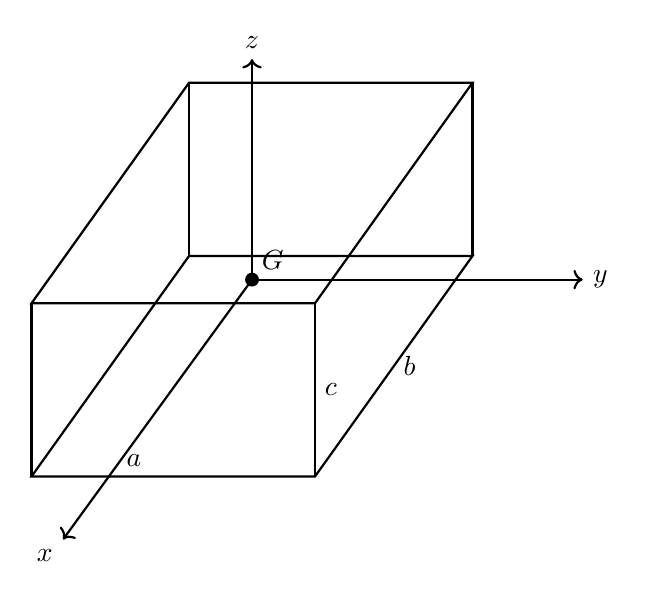
\begin{tikzpicture}[scale=1]
  % centro di massa
  \coordinate (G) at (0,0);

  % direzioni degli spigoli
  \coordinate (ex) at (-2.0,-2.8);
  \coordinate (ey) at (3.6,0);
  \coordinate (ez) at (0,2.2);

  % vertici del parallelepipedo
  \coordinate (A) at ($(G)+0.5*(ex)-0.5*(ey)-0.5*(ez)$);
  \coordinate (B) at ($(G)-0.5*(ex)-0.5*(ey)-0.5*(ez)$);
  \coordinate (C) at ($(G)-0.5*(ex)+0.5*(ey)-0.5*(ez)$);
  \coordinate (D) at ($(G)+0.5*(ex)+0.5*(ey)-0.5*(ez)$);
  \coordinate (E) at ($(G)+0.5*(ex)-0.5*(ey)+0.5*(ez)$);
  \coordinate (F) at ($(G)-0.5*(ex)-0.5*(ey)+0.5*(ez)$);
  \coordinate (H) at ($(G)-0.5*(ex)+0.5*(ey)+0.5*(ez)$);
  \coordinate (I) at ($(G)+0.5*(ex)+0.5*(ey)+0.5*(ez)$);

  % parallelepipedo
  \draw[thick] (A)--(B)--(C)--(D)--cycle;
  \draw[thick] (E)--(F)--(H)--(I)--cycle;
  \draw[thick] (A)--(E);
  \draw[thick] (B)--(F);
  \draw[thick] (C)--(H);
  \draw[thick] (D)--(I);

  % punto G
  \fill (G) circle (2.5pt);
  \node[above right] at (G) {$G$};

  % assi nel centro di massa
  \draw[thick,->] (G) -- ($(G)+(0,2.8)$) node[above] {$z$};
  \draw[thick,->] (G) -- ($(G)+(4.2,0)$) node[right] {$y$};
  \draw[thick,->] (G) -- ($(G)+(-2.4,-3.3)$) node[below left] {$x$};

  % etichette lati
  \node[below] at ($(G)+0.75*(ex)$) {$a$};
  \node[right] at ($(D)!0.5!(C)$) {$b$};
  \node[right] at ($(I)!0.5!(D)$) {$c$};
\end{tikzpicture}
\end{center}

\[
(I_G)_{11}
=
\int_{\Omega}(y^2+z^2)\rho\, dv
=
\int_{-\frac{a}{2}}^{\frac{a}{2}}
\int_{-\frac{b}{2}}^{\frac{b}{2}}
\int_{-\frac{c}{2}}^{\frac{c}{2}}
\rho\,(y^2+z^2)\,dz\,dy\,dx
=
\]

\[
=
\rho
\int_{-\frac{a}{2}}^{\frac{a}{2}}
\int_{-\frac{b}{2}}^{\frac{b}{2}}
\left[
y^2z+\frac{z^3}{3}
\right]_{-\frac{c}{2}}^{\frac{c}{2}}
\,dy\,dx
=
\]

\[
=
\rho
\int_{-\frac{a}{2}}^{\frac{a}{2}}
\int_{-\frac{b}{2}}^{\frac{b}{2}}
y^2\frac{c}{2}
+\frac{c^3}{8}\frac{1}{3}
+y^2\frac{c}{2}
+\frac{c^3}{8}\frac{1}{3}
\,dy\,dx
=
\]

\[
=
\frac{m}{abc}\cdot a
\int_{-\frac{b}{2}}^{\frac{b}{2}}
y^2c+\frac{c^3}{12}
\,dy
=
\frac{m}{bc}\cdot
\left[
\frac{y^3}{3}c+\frac{c^3}{12}y
\right]_{-\frac{b}{2}}^{\frac{b}{2}}
=
\]

\[
=
\frac{m}{bc}\cdot 2
\left(
\frac{b^3}{8}\cdot\frac{c}{3}
+
\frac{c^3}{12}\cdot\frac{b}{2}
\right)
=
\frac{2m}{bc}
\left(
\frac{b^3c}{24}
+
\frac{c^3b}{24}
\right)
=
\]

\[
=
\frac{m}{bc}
\left(
\frac{b^3c}{12}
+
\frac{c^3b}{12}
\right)
=
m\left(
\frac{b^2}{12}
+
\frac{c^2}{12}
\right)
=
\frac{m(b^2+c^2)}{12}
\]

\[
\Rightarrow\quad
I_G=
\left(
\begin{array}{ccc}
\dfrac{m(b^2+c^2)}{12} & 0 & 0 \\[0.8em]
0 & \dfrac{m(a^2+c^2)}{12} & 0 \\[0.8em]
0 & 0 & \dfrac{m(a^2+b^2)}{12}
\end{array}
\right)
\]

Gli assi paralleli ai lati sono quindi gli assi principali d'inerzia.
\end{example}







\begin{example}{}
\(I_G\) di un disco di raggio \(R\) e densità superficiale
\[
\rho=\frac{m}{\pi R^2}
\]

\[
I_G^{zz}=I_G=\int_{\Omega}(y^2+x^2)\rho\, dx\,dy
=
\int_{0}^{R} r\int_{0}^{2\pi} r^2\rho\, d\theta\,dr
=
\int_{0}^{R} r^3\rho\,2\pi\,dr
=
\]

\[
=
\frac{m}{\pi R^2}\cdot 2\pi \cdot \left[\frac{r^4}{4}\right]_{0}^{R}
=
\frac{2m}{R^2}\cdot \frac{R^4}{4}
=
\frac{1}{2}mR^2
\]
\end{example}


\begin{example}{}
Nell'esempio precedente abbiamo calcolato \(I_G\) per un disco piano.
Facciamolo anche per un anello di raggio \(R\) e massa \(m\).

Modellizziamo l'anello come una circonferenza di raggio \(R\).
Non possiamo utilizzare un integrale doppio perché integrare su un insieme di
misura di Peano-Jordan nulla darebbe un integrale nullo.

Definiamo
\[
\lambda=\frac{m}{2\pi R}
\]
densità lineare costante. Allora, dette
\[
\gamma(t)=(R\cos t,\;R\sin t),
\]
si ha
\[
\gamma'(t)=(-R\sin t,\;R\cos t),
\qquad
\|\gamma'(t)\|=\sqrt{R^2\sin^2 t+R^2\cos^2 t}=R.
\]

Si ha quindi
\[
I_G=\int_{\gamma}(x^2+y^2)\lambda\,ds
=\int_0^{2\pi} R^2(\sin^2 t+\cos^2 t)\cdot \lambda \cdot R\,dt
=\int_0^{2\pi} R^2\cdot \frac{m}{2\pi R}\cdot R\,dt
\]
\[
=R^2m\cdot \frac{2\pi}{2\pi}=mR^2.
\]

Il momento d'inerzia di un anello, a parità di massa e raggio, è doppio rispetto
a quello di un disco. Questo vuol dire che per ottenere lo stesso moto bisogna
applicare un momento più alto nell'anello rispetto al disco. Intuitivamente
questo ha senso perché l'anello ha una configurazione di massa mediamente più
distante dal centro di massa rispetto al disco.

Nella prima equazione cardinale invece non ci sono differenze tra i due, a
riprova del fatto che il centro di massa si muove indipendentemente dalla
configurazione di massa del corpo rigido.
\end{example}



Vogliamo ora ottenere la seconda legge cardinale per un polo qualsiasi.
Consideriamo un sistema di \(n\) punti materiali legati dai vincoli del corpo
rigido e caratterizzato da \(m_i,\ \underline{x}_i\), \(\forall i=1,\dots,n\).
Sia inoltre un polo \(\underline{x}_p(t)\in\mathbb{R}^3\).

Per ogni punto vale
\[
m_i\,\underline{\ddot{x}}_i=\underline{f}_i.
\]
Allora
\[
\underline{x}_p\wedge m_i\,\frac{d}{dt}\bigl(\underline{v}_i\bigr)
=
\underline{x}_p\wedge \underline{f}_i.
\]

Sommando su \(i\) otteniamo
\[
\sum_{i=1}^n \underline{x}_p\wedge m_i\,\frac{d}{dt}\bigl(\underline{v}_i\bigr)
=
\underline{x}_p\wedge \frac{d}{dt}\bigl(m\,\underline{v}_G\bigr)
=
\underline{x}_p\wedge \sum_{i=1}^n \underline{f}_i^{\mathrm{ext}}.
\]

La sottraggo alla seconda equazione cardinale
\[
\frac{d}{dt}\Bigl(\underline{x}_G\wedge m\,\underline{v}_G+I_G\underline{\omega}\Bigr)
-
\underline{x}_p\wedge \frac{d}{dt}\bigl(m\,\underline{v}_G\bigr)
=
\sum_{i=1}^n (\underline{x}_i-\underline{x}_p)\wedge \underline{f}_i^{\mathrm{ext}}.
\]

Deriviamo la quantità \(\underline{x}_p\wedge m\,\underline{v}_G\) nel tempo
\[
\frac{d}{dt}\Bigl(\underline{x}_p\wedge m\,\underline{v}_G\Bigr)
=
\underline{v}_p\wedge m\,\underline{v}_G
+
\underline{x}_p\wedge \frac{d}{dt}\bigl(m\,\underline{v}_G\bigr)
\]
\[
\Rightarrow\quad
-
\underline{x}_p\wedge \frac{d}{dt}\bigl(m\,\underline{v}_G\bigr)
=
\underline{v}_p\wedge m\,\underline{v}_G
-
\frac{d}{dt}\Bigl(\underline{x}_p\wedge m\,\underline{v}_G\Bigr).
\]

Sostituendo in alto si ottiene
\[
\frac{d}{dt}\Bigl(\underline{x}_G\wedge m\,\underline{v}_G+I_G\underline{\omega}\Bigr)
+
\underline{v}_p\wedge m\,\underline{v}_G
-
\frac{d}{dt}\Bigl(\underline{x}_p\wedge m\,\underline{v}_G\Bigr)
=
\sum_{i=1}^n (\underline{x}_i-\underline{x}_p)\wedge \underline{f}_i^{\mathrm{ext}}.
\]

Riorganizzando i termini si ottiene la seconda legge cardinale della dinamica
del corpo rigido rispetto a un polo qualsiasi
\[
\frac{d}{dt}\Bigl((\underline{x}_G-\underline{x}_p)\wedge m\,\underline{v}_G
+
I_G\underline{\omega}\Bigr)
=
\sum_{i=1}^n (\underline{x}_i-\underline{x}_p)\wedge \underline{f}_i^{\mathrm{ext}}
-
\underline{v}_p\wedge m\,\underline{v}_G.
\]

Se indichiamo con
\[
\underline{L}_{G,p}=(\underline{x}_G-\underline{x}_p)\wedge m\,\underline{v}_G
\]
il momento angolare del centro di massa rispetto al polo \(p\) e
\[
\underline{M}_{i,p}^{\mathrm{ext}}=(\underline{x}_i-\underline{x}_p)\wedge \underline{f}_i^{\mathrm{ext}}
\]
il momento delle forze esterne agenti su \(\underline{x}_i\) rispetto al polo \(p\),
l'equazione diventa
\[
\frac{d}{dt}\Bigl(\underline{L}_{G,p}+I_G\underline{\omega}\Bigr)
=
\sum_{i=1}^n \underline{M}_{i,p}^{\mathrm{ext}}
-
\underline{v}_p\wedge m\,\underline{v}_G.
\]


\begin{oss}{}
Il termine \(\underline{v}_p \wedge m\,\underline{v}_G\) si annulla se:
\begin{enumerate}[label=\roman*)]
    \item \(\underline{v}_p \parallel \underline{v}_G\);
    \item \(\underline{x}_p\) è un polo fisso;
    \item \(\underline{x}_p=\underline{x}_G\), ovvero il polo è il centro di massa.
\end{enumerate}

Spesso quindi si sceglie \(\underline{x}_p=\underline{x}_G\) e in tal caso ritroviamo
\[
\frac{d}{dt}\bigl(I_G\underline{\omega}\bigr)
=
\sum_{i=1}^{n} (\underline{x}_i-\underline{x}_G)\wedge \underline{f}_i^{\mathrm{ext}}
\qquad \Longleftrightarrow \qquad
\frac{d}{dt}\Bigl(\underline{x}_G\wedge m\,\underline{v}_G+I_G\underline{\omega}\Bigr)
=
\sum_{i=1}^{n} \underline{x}_i\wedge \underline{f}_i^{\mathrm{ext}}.
\]

\medskip

La prima equazione cardinale non dipende da poli o punti di applicazione
delle forze. La seconda invece varia a seconda del polo e dei punti di
applicazione delle forze.
\end{oss}

\section{Coppia di forze di momento M}
\begin{definition}{}
Una coppia di forze è definita da due forze che hanno
\begin{itemize}
    \item stesso modulo;
    \item verso opposto;
    \item agiscono su rette parallele.
\end{itemize}
\end{definition}
\begin{center}
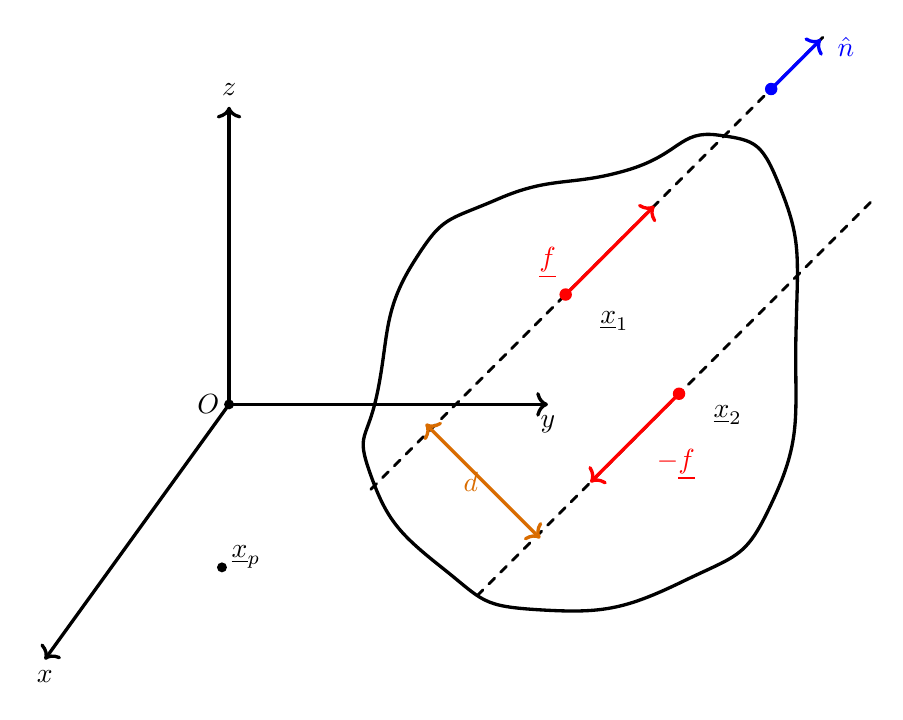
\begin{tikzpicture}[scale=0.9, line cap=round, line join=round]

% Assi
\coordinate (O) at (0,0);
\fill (O) circle (2pt);
\node[left] at (O) {$O$};

\draw[->, very thick] (O) -- (0,4.2) node[above] {$z$};
\draw[->, very thick] (O) -- (4.5,0) node[below] {$y$};
\draw[->, very thick] (O) -- (-2.6,-3.6) node[below] {$x$};

% Punto x_p
\fill (-0.1,-2.3) circle (2pt);
\node[right] at (-0.1,-2.15) {$\underline{x}_p$};

% Contorno del corpo
\draw[very thick]
plot[smooth cycle, tension=0.9] coordinates {
    (2.1,0.2)
    (2.6,2.0)
    (3.8,2.9)
    (5.6,3.3)
    (6.9,3.8)
    (7.8,3.0)
    (8.0,1.0)
    (7.7,-1.3)
    (6.4,-2.5)
    (4.4,-2.9)
    (3.0,-2.3)
    (2.0,-1.0)
};

% Rette parallele tratteggiate
\draw[dashed, line width=1pt] (2.0,-1.2) -- (8.4,5.2);
\draw[dashed, line width=1pt] (3.5,-2.7) -- (9.1,2.9);

% Versore m con punto blu
\fill[blue] (7.65,4.45) circle (2.5pt);
\draw[->, very thick, blue] (7.65,4.45) -- (8.35,5.15);
\node[blue, right] at (8.45,5.05) {$\hat n$};

% Forza superiore
\fill[red] (4.75,1.55) circle (2.5pt);
\draw[->, very thick, red] (4.75,1.55) -- (6,2.8);
\node[red, left] at (4.75,2.0) {$\underline{f}$};
\node[black, below right] at (5.1,1.45) {$\underline{x}_1$};

% Forza inferiore
\fill[red] (6.35,0.15) circle (2.5pt);
\draw[->, very thick, red] (6.35,0.15) -- (5.1,-1.1);
\node[red, right] at (5.9,-0.85) {$-\underline{f}$};
\node[black, right] at (6.7,-0.15) {$\underline{x}_2$};

% Distanza d tra le rette

\draw[<->, very thick, orange!85!black] (4.39, -1.89) -- (2.775 ,  -0.275);
\node[orange!85!black, left] at (3.65,-1.1) {$d$};

\end{tikzpicture}
\end{center}

Calcoliamo il momento delle forze generato dalla coppia di forze rispetto al polo $\underline{x}_p$:
\[
\underline{M}
=
(\underline{x}_1-\underline{x}_p)\wedge f\,\hat n
+
(\underline{x}_2-\underline{x}_p)\wedge (-f\,\hat n)
=
(\underline{x}_1-\underline{x}_2)\wedge f\,\hat n
\]

Quindi il momento generato da una coppia di forze è indipendente dal polo e dipende soltanto dal prodotto dell'intensità della forza e la distanza tra le rette di applicazione. Infatti
\[
\|\underline{M}\| = f\,\|\underline{x}_1-\underline{x}_2\|\sin\alpha = fd
\]

Il vettore $\underline{M}$ è ortogonale al piano su cui giacciono le forze.
È quindi lecito parlare di \textbf{coppia di forze di momento $M$ con verso orario/antiorario}.

\begin{example}{}
Consideriamo un disco che rotola nel piano soggetto ad un momento $M$ orario. Il disco ha massa $m$ e raggio $R$.

\begin{figure}
\centering
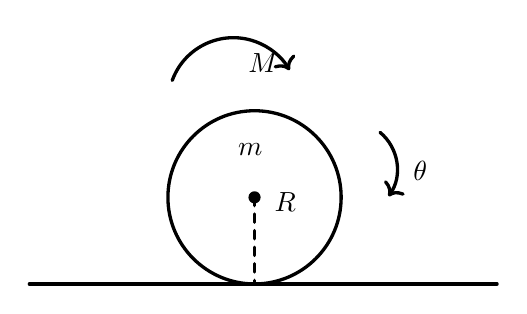
\begin{tikzpicture}[scale=1.1, line cap=round, line join=round]

% Suolo
\draw[very thick] (-2.6,0) -- (2.8,0);

% Disco
\def\R{1.0}
\coordinate (C) at (0,\R);
\draw[very thick] (C) circle (\R);

% Centro e massa
\fill (C) circle (2pt);
\node at (-0.05,1.55) {$m$};

% Raggio tratteggiato
\draw[dashed, very thick] (C) -- (0,0);
\node[right] at (0.12,0.95) {$R$};

% Momento M in senso orario sopra il disco
\draw[->, very thick] (-0.95,2.35) arc[start angle=160,end angle=30,radius=0.75];
\node at (0.1,2.55) {$M$};

% Rotazione theta a destra in senso orario
\draw[->, very thick] (1.45,1.75) arc[start angle=50,end angle=-35,radius=0.55];
\node[right] at (1.72,1.3) {$\theta$};

\end{tikzpicture}
\end{figure}

Applichiamo la seconda legge cardinale scegliendo come polo il punto di contatto $C$:
\[
\frac{d}{dt}\bigl(I_C\omega\bigr)=\sum_{i=1}^{n}(\underline{x}_i-C)\wedge \underline{f}_i
\]

Dal momento che ci è stato dato un momento $\underline{M}$ possiamo supporre che questo venga generato da una coppia di forze parallele e quindi il suo valore sia indipendente dal polo scelto:
\[
\underline{M}
=
\sum_{i=1}^{n}(\underline{x}_i-\underline{x}_p)\wedge \underline{f}_i
=
(\underline{x}_1-\underline{x}_p)\wedge \underline{f}
+
(\underline{x}_2-\underline{x}_p)\wedge (-\underline{f})
\qquad \forall\,\underline{x}_p.
\]

In particolare, scegliendo $\underline{x}_p=C$ e ricordando che per il teorema di Huygens-Steiner il momento d'inerzia di un disco rispetto al punto di contatto è $I_C = I_G + mR^2 = \frac{1}{2}mR^2 + mR^2 = \frac{3}{2}mR^2$, possiamo scrivere:
\[
\frac{d}{dt}\left(\frac{3}{2}mR^2\dot{\theta}\right)=M
\qquad \Longrightarrow \qquad
\frac{3}{2}mR^2\ddot{\theta}=M
\]
\end{example}
\section{Il Teorema di Huygens}

Il seguente teorema è utile per corpi rigidi che ruotano attorno a punti o
assi fissi. Enunciamo e dimostriamo una versione del teorema per moti piani.
\begin{theorem}{}[Teorema di Huygens]
Consideriamo un corpo rigido nel piano che ruota attorno ad un punto fisso
\(\underline{x}_p\). Allora la seconda equazione cardinale rispetto al polo
\(\underline{x}_p\) si scrive nella forma
\[
\frac{d}{dt}\bigl(I_p\underline{\omega}\bigr)
=
\sum_{i=1}^{n} (\underline{x}_i-\underline{x}_p)\wedge \underline{f}_i^{\mathrm{ext}}
\]
con
\[
I_p=I_G+ma^2,
\qquad
a^2=\|\underline{x}_p-\underline{x}_G\|^2.
\]
\end{theorem}

\begin{proof}
Scriviamo la seconda equazione cardinale rispetto al polo \(\underline{x}_p\)
\[
\frac{d}{dt}\Bigl((\underline{x}_G-\underline{x}_p)\wedge m\underline{v}_G+I_G\underline{\omega}\Bigr)
=
\sum_{i=1}^{n} (\underline{x}_i-\underline{x}_p)\wedge \underline{f}_i^{\mathrm{ext}}
-
\underline{v}_p\wedge m\underline{v}_G.
\]

Notiamo che \(\underline{v}_p=\underline{0}\), quindi
\[
-\underline{v}_p\wedge m\underline{v}_G=\underline{0}.
\]

Inoltre uso la formula fondamentale della cinematica per \(\underline{x}_p\) e
\(\underline{x}_G\)
\[
\underline{v}_G=\underline{v}_p+\underline{\omega}\wedge(\underline{x}_G-\underline{x}_p)
=
\underline{\omega}\wedge(\underline{x}_G-\underline{x}_p).
\]

Sostituendo si ottiene
\[
\frac{d}{dt}\Bigl((\underline{x}_G-\underline{x}_p)\wedge
m\bigl(\underline{\omega}\wedge(\underline{x}_G-\underline{x}_p)\bigr)
+
I_G\underline{\omega}\Bigr)
=
\sum_{i=1}^{n} (\underline{x}_i-\underline{x}_p)\wedge \underline{f}_i^{\mathrm{ext}}.
\]

Uso la formula
\[
\underline{a}\wedge(\underline{b}\wedge \underline{a})
=
\underline{b}\,(\underline{a}\cdot \underline{a})
-
\underline{a}\,(\underline{a}\cdot \underline{b})
\]
con
\[
\underline{a}=\underline{x}_G-\underline{x}_p,
\qquad
\underline{b}=m\underline{\omega}.
\]
Allora
\[
(\underline{x}_G-\underline{x}_p)\wedge
m\bigl(\underline{\omega}\wedge(\underline{x}_G-\underline{x}_p)\bigr)
=
m\underline{\omega}\,\|\underline{x}_G-\underline{x}_p\|^2
-
(\underline{x}_G-\underline{x}_p)\bigl(m\underline{\omega}\cdot(\underline{x}_G-\underline{x}_p)\bigr).
\]
Poiché \(\underline{\omega}\perp(\underline{x}_G-\underline{x}_p)\), il secondo
termine si annulla e quindi
\[
(\underline{x}_G-\underline{x}_p)\wedge
m\bigl(\underline{\omega}\wedge(\underline{x}_G-\underline{x}_p)\bigr)
=
m\underline{\omega}\,\|\underline{x}_G-\underline{x}_p\|^2.
\]

Allora
\[
\frac{d}{dt}\Bigl(m\|\underline{x}_G-\underline{x}_p\|^2\underline{\omega}
+
I_G\underline{\omega}\Bigr)
=
\sum_{i=1}^{n} (\underline{x}_i-\underline{x}_p)\wedge \underline{f}_i^{\mathrm{ext}}.
\]

Imponendo
\[
I_p=m\|\underline{x}_G-\underline{x}_p\|^2+I_G
\]
otteniamo
\[
\frac{d}{dt}\bigl(I_p\underline{\omega}\bigr)
=
\sum_{i=1}^{n} (\underline{x}_i-\underline{x}_p)\wedge \underline{f}_i^{\mathrm{ext}}.
\]
\end{proof}


\section{Esempi applicativi}
\begin{example}{}
Consideriamo un'asta con un estremo fissato, massa \(m\) e lunghezza \(\ell\).

\begin{figure}
\centering
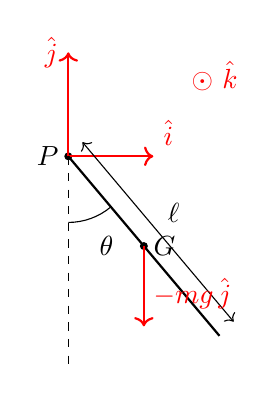
\begin{tikzpicture}[scale=1.2]
    % punto P
    \fill (0,0) circle (1.2pt);
    \node[left] at (0,0) {\(P\)};

    % assi
    \draw[red,->,thick] (0,0) -- (0.9,0) node[above right] {\(\hat{i}\)};
    \draw[red,->,thick] (0,0) -- (0,1.1) node[left] {\(\hat{j}\)};
    \node[red] at (1.55,0.85) {\(\odot\ \hat{k}\)};

    % verticale tratteggiata
    \draw[dashed] (0,0) -- (0,-2.2);

    % asta
    \draw[thick] (0,0) -- (1.6,-1.9);
    \draw[<->] (0.15,0.15) -- node[above right] {\(\ell\)} (1.75,-1.75);

    % centro di massa G
    \fill (0.8,-0.95) circle (1.2pt);
    \node[right] at (0.8,-0.95) {\(G\)};

    % forza peso
    \draw[red,->,thick] (0.8,-0.95) -- (0.8,-1.8);
    \node[right,red] at (0.8,-1.45) {\(-mg\,\hat{j}\)};

    % angolo theta
    \draw (0,-0.7) arc[start angle=-90,end angle=-50,radius=0.7];
    \node[left] at (0.58,-0.95) {\(\theta\)};
\end{tikzpicture}
\end{figure}

Imponiamo i vincoli
\[
\underline{x}_p=(k_1,k_2,0).
\]
Il sistema ha quindi \(3-2=1\) grado di libertà. Scriviamo la seconda legge
cardinale rispetto al polo \(p\):
\[
\frac{d}{dt}\bigl(I_p\dot{\theta}\bigr)
=
\frac{d}{dt}\bigl((I_G+ma^2)\dot{\theta}\bigr)
=
\frac{d}{dt}\left(\left(\frac{m\ell^2}{12}+m\left(\frac{\ell}{2}\right)^2\right)\dot{\theta}\right)
=
(\underline{x}_G-\underline{x}_p)\wedge(-mg\,\hat{j}).
\]

\[
\Rightarrow\quad
\frac{d}{dt}\left(\left(\frac{m\ell^2}{12}+\frac{m\ell^2}{4}\right)\dot{\theta}\right)
=
-\frac{\ell}{2}\,mg\,\sin(\pi-\theta)\,\hat{k}
=
-\frac{\ell}{2}\,mg\,\sin\theta\,\hat{k}.
\]

\[
\Rightarrow\quad
\frac{d}{dt}\left(\frac{m\ell^2}{3}\dot{\theta}\right)
=
-\frac{\ell}{2}\,mg\,\sin\theta
\Rightarrow
\frac{\ell}{3}\ddot{\theta}
=
-\frac{g}{2}\sin\theta
\Rightarrow
\ddot{\theta}
=
-\frac{3}{2}\frac{g}{\ell}\sin\theta.
\]

L'ultima equazione differenziale si risolve con il metodo delle funzioni
ellittiche.

Notiamo che la soluzione \(\theta(t)\) non può dipendere dalla massa.

Sotto l'ipotesi delle piccole oscillazioni \(\left(\theta\ll \frac{\pi}{2}\right)\)
allora
\[
\sin\theta=\theta+o(\theta^2),
\]
cioè possiamo linearizzare il problema:
\[
\ddot{\theta}
=
-\frac{3}{2}\frac{g}{\ell}\theta,
\qquad
\omega^2=\frac{3}{2}\frac{g}{\ell}
\]
\[
\Rightarrow\quad
\ddot{\theta}+\omega^2\theta=0
\Rightarrow
\lambda^2+\omega^2=0
\Rightarrow
\lambda=\pm i\omega.
\]

\[
\Rightarrow\quad
\theta(t)=A\cos(\omega t+\varphi),
\qquad
A \text{ e } \varphi \text{ fissate dalle condizioni iniziali.}
\]


\begin{oss}{}
Avremmo potuto ricavare \(\theta(t)\) anche attraverso la prima equazione
cardinale. Partiamo da
\[
\begin{cases}
x_G=\dfrac{\ell}{2}\sin\theta\\[4pt]
y_G=-\dfrac{\ell}{2}\cos\theta
\end{cases}
\qquad \Rightarrow \qquad
\begin{cases}
v_G^x=\dot{\theta}\,\dfrac{\ell}{2}\cos\theta\\[4pt]
v_G^y=\dot{\theta}\,\dfrac{\ell}{2}\sin\theta
\end{cases}
\qquad \Rightarrow \qquad
\begin{cases}
a_G^x=\dfrac{\ell}{2}\cos\theta\,\ddot{\theta}-\dfrac{\ell}{2}\sin\theta\,\dot{\theta}^2\\[4pt]
a_G^y=\dfrac{\ell}{2}\sin\theta\,\ddot{\theta}+\dfrac{\ell}{2}\cos\theta\,\dot{\theta}^2
\end{cases}
\]

\[
\Rightarrow
\begin{cases}
m\left[\dfrac{\ell}{2}\cos\theta\,\ddot{\theta}-\dfrac{\ell}{2}\sin\theta\,\dot{\theta}^2\right]=R_x\\[8pt]
m\left[\dfrac{\ell}{2}\sin\theta\,\ddot{\theta}+\dfrac{\ell}{2}\cos\theta\,\dot{\theta}^2\right]=-mg+R_y
\end{cases}
\]

dove
\[
\underline{R}=R_x\hat{i}+R_y\hat{j}
\]
è la reazione vincolare dovuta al vincolo in \(\underline{x}_p\), il cui momento
rispetto a \(\underline{x}_p\) è nullo e che quindi abbiamo ignorato nei calcoli
precedenti.

Se al sistema di equazioni che abbiamo trovato aggiungiamo
\[
\frac{d}{dt}\bigl(I_G\dot{\theta}\bigr)=-\underline{x}_G\wedge \underline{R}
\qquad \Longleftrightarrow \qquad
\frac{d}{dt}\left(\frac{m\ell^2}{12}\dot{\theta}\,\hat{k}\right)
=
-\left[\frac{\ell}{2}R_x\cos\theta+\frac{\ell}{2}R_y\sin\theta\right]\hat{k}
\]
otteniamo \(3\) equazioni indipendenti per le \(3\) incognite scalari
\(\theta\), \(R_x\), \(R_y\).

È indubbiamente evidente la facilità del primo procedimento rispetto a
quest'ultimo.
\end{oss}

\end{example}


\begin{example}{}
Consideriamo un disco di massa \(m\) e raggio \(R\) vincolato a muoversi
in un piano verticale. Al centro di massa del disco è attaccata una
molla a riposo. Il disco si muove di puro rotolamento rispetto al
terreno. Sia \(K\) la costante elastica della molla.

\begin{figure}
\centering
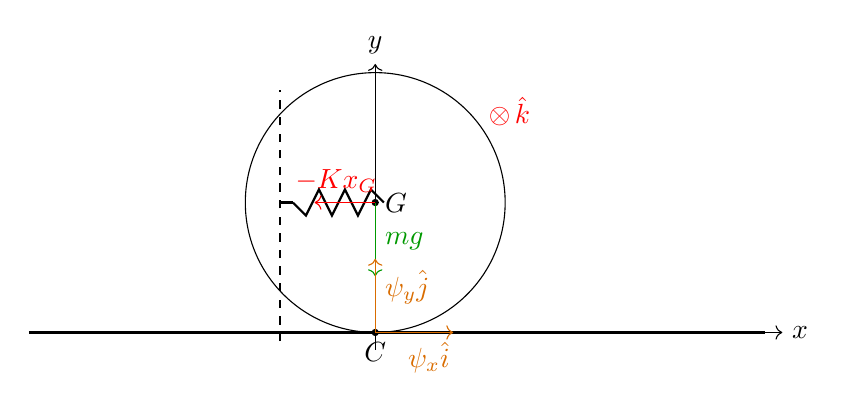
\begin{tikzpicture}[scale=1.1]
    % terreno
    \draw[thick] (-4,0) -- (4.5,0);
    \draw[->] (0,0) -- (4.7,0) node[right] {\(x\)};

    % asse y
    \draw[->] (0,-0.2) -- (0,3.1) node[above] {\(y\)};

    % disco
    \draw (0,1.5) circle (1.5);

    % centro e punto di contatto
    \fill (0,1.5) circle (1.2pt);
    \node[right] at (0,1.5) {\(G\)};
    \fill (0,0) circle (1.2pt);
    \node[below] at (0,0) {\(C\)};

    % linea tratteggiata
    \draw[dashed] (-1.1,-0.1) -- (-1.1,2.8);

    % molla
    \draw[thick] (-1.1,1.5) -- (-0.95,1.5);
    \draw[thick] (-0.95,1.5) -- (-0.8,1.35) -- (-0.65,1.65) -- (-0.5,1.35) -- (-0.35,1.65) -- (-0.2,1.35) -- (-0.05,1.65) -- (0.1,1.5);

    % versore k entrante
    \node[red] at (1.55,2.55) {\(\otimes\,\hat{k}\)};

    % forza elastica
    \draw[red,->] (0,1.5) -- (-0.7,1.5);
    \node[red,above] at (-0.45,1.5) {\(-Kx_G\)};

    % peso
    \draw[green!60!black,->] (0,1.5) -- (0,0.65);
    \node[green!60!black,right] at (0,1.05) {\(mg\)};

    % reazioni vincolari
    \draw[orange!85!black,->] (0,0) -- (0.9,0);
    \node[orange!85!black,below] at (0.62,0) {\(\psi_x\hat{i}\)};

    \draw[orange!85!black,->] (0,0) -- (0,0.85);
    \node[orange!85!black,right] at (0,0.52) {\(\psi_y\hat{j}\)};
\end{tikzpicture}
\end{figure}

Impongo i vincoli di puro rotolamento
\[
\underline{v}_C=\underline{0}
\quad \Rightarrow \quad
v_C^x=v_C^y=0
\quad \Rightarrow \quad
\text{il sistema ha } 3-2=1 \text{ grado di libertà.}
\]

In un moto di puro rotolamento vale
\[
\dot{x}_G=R\dot{\theta}
\quad \Rightarrow \quad
x_G=R\theta+C.
\]
Per la nostra configurazione \(C=0\).

Impostiamo la prima legge cardinale
\[
\begin{cases}
m\ddot{x}_G=-Kx_G+\psi_x,\\[4pt]
m\ddot{y}_G=-mg+\psi_y.
\end{cases}
\]

Dal momento che le forze lungo \(\hat{j}\) sono parallele al braccio non c'è
momento. Lo stesso vale per la forza elastica che ha braccio nullo.
Nella seconda equazione cardinale rispetto a \(G\) rimane solo
\[
(\underline{x}_C-\underline{x}_G)\wedge \psi_x\hat{i}
=
-R\psi_x\hat{k}
\quad \Rightarrow \quad
\frac{d}{dt}\bigl(I_G\dot{\theta}\bigr)=-R\psi_x.
\]

Dobbiamo quindi risolvere il sistema
\[
\begin{cases}
m\ddot{x}_G=-Kx_G+\psi_x,\\[4pt]
m\ddot{y}_G=-mg+\psi_y,\\[4pt]
\dfrac{d}{dt}\bigl(I_G\dot{\theta}\bigr)=-R\psi_x.
\end{cases}
\]

Ma
\[
x_G=R\theta,\qquad \ddot{y}_G=0,\qquad I_G=\frac{mR^2}{2}
\]
e quindi
\[
\begin{cases}
mR\ddot{\theta}=-KR\theta+\psi_x,\\[4pt]
0=-mg+\psi_y,\\[4pt]
\dfrac{mR}{2}\ddot{\theta}=-R\psi_x.
\end{cases}
\]

Sistema di \(3\) equazioni nelle \(3\) incognite \(\psi_x,\psi_y,\theta\).
\end{example}


\begin{example}{}
Consideriamo un'asta di lunghezza \(\ell\) e massa \(m\) collegata all'estremo
superiore ad una molla di costante elastica \(K\).
\begin{center}
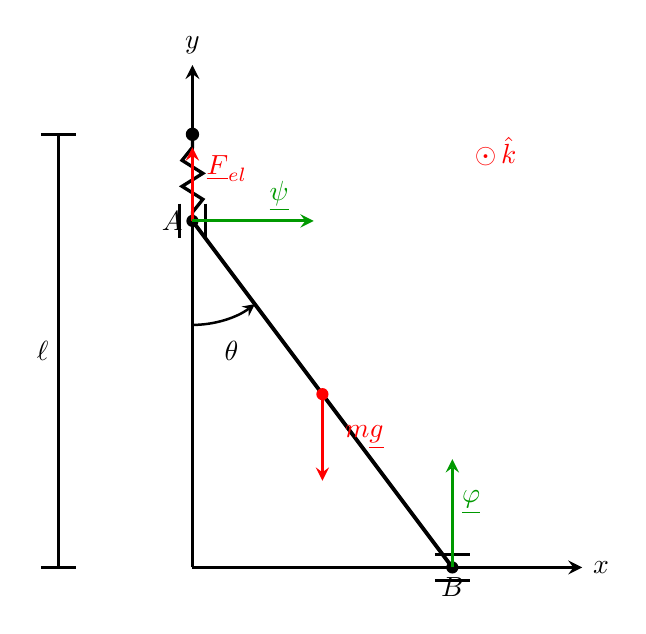
\begin{tikzpicture}[scale=1.1, >=stealth]
    % assi
    \draw[->,line width=1.2pt] (0,0) -- (4.5,0) node[right] {$x$};
    \draw[->,line width=1.2pt] (0,0) -- (0,5.8) node[above] {$y$};

    % Punti calcolati con terna pitagorica 3-4-5 per un rigore matematico assoluto!
    % Lunghezza asta = 5, quota soffitto \ell = 5
    \coordinate (A) at (0,4);
    \coordinate (B) at (3,0);
    \coordinate (G) at ($(A)!0.5!(B)$);
    \coordinate (S1) at (0,5); % Soffitto a quota 5

    % quota \ell (altezza 5)
    \draw[line width=1.2pt] (-1.55,0) -- (-1.55,5.0);
    \draw[line width=1.2pt] (-1.75,0) -- (-1.35,0);
    \draw[line width=1.2pt] (-1.75,5.0) -- (-1.35,5.0);
    \node[left] at (-1.55,2.5) {$\ell$};

    % guida verticale in A
    \draw[line width=1.3pt] (-0.15,4.2) -- (-0.15,3.8);
    \draw[line width=1.3pt] ( 0.15,4.2) -- ( 0.15,3.8);

    % guida orizzontale in B
    \draw[line width=1.3pt] (2.8, 0.15) -- (3.2, 0.15);
    \draw[line width=1.3pt] (2.8,-0.15) -- (3.2,-0.15);

    % asta
    \draw[line width=1.4pt] (A) -- (B);

    % molla disegnata a zig-zag proporzionato tra Soffitto(5.0) e A(4.0)
    \fill (S1) circle (2.2pt);
    \draw[line width=1.2pt] (S1) -- (0,4.85) -- (-0.12,4.7) -- (0.12,4.55) -- (-0.12,4.4) -- (0.12,4.25) -- (0,4.1) -- (A);

    % punti A, B, G
    \fill (A) circle (2pt);
    \fill (B) circle (2pt);
    \fill[red] (G) circle (2pt);

    \node[left] at (A) {$A$};
    \node[below] at (B) {$B$};

    % forze attive
    \draw[->,red,line width=1.1pt] (A) -- ++(0,0.85);
    \node[red,right] at ($(A)+(0.05,0.6)$) {$\underline{F}_{el}$};

    \draw[->,red,line width=1.1pt] (G) -- ++(0,-1.0);
    \node[red,right] at ($(G)+(0.15,-0.5)$) {$m\underline{g}$};

    % reazioni vincolari incognite
    \draw[->,green!60!black,line width=1.1pt] (A) -- ++(1.4,0);
    \node[green!60!black,above] at ($(A)+(1.0,0)$) {$\underline{\psi}$};

    \draw[->,green!60!black,line width=1.1pt] (B) -- ++(0,1.25);
    \node[green!60!black,right] at ($(B)+(0,0.75)$) {$\underline{\varphi}$};

    % angolo theta: posizionato e calcolato in modo esatto
    % Con i cateti a 3 e 4, l'angolo d'inclinazione è di circa 53.13 gradi
    \draw[->,line width=0.9pt] (0,2.8) arc[start angle=-90,end angle=-53.13,radius=1.2];
    \node at (0.45, 2.5) {$\theta$};

    % versore k uscente
    \node[red] at (3.5,4.8) {$\odot\,\hat{k}$};

\end{tikzpicture}
\end{center}


L'asta è soggetta ai vincoli
\[
x_A=0,\qquad y_B=0
\]
e ha quindi \(3-2=1\) grado di libertà. Inoltre la molla è a riposo per
\(\theta=0\). Scegliamo \(\theta(t)\) come coordinata libera.

Le forze attive sono
\[
\underline{F}_{el}=K(\ell-\ell\cos\theta)\,\hat{j},
\qquad
-mg\,\hat{j}.
\]

Le forze vincolari incognite sono \(\psi\,\hat{i}\) applicata in \(A\) e
\(\varphi\,\hat{j}\) applicata in \(B\).

Impostiamo la prima equazione cardinale
\[
\frac{d}{dt}\bigl(m\underline{v}_G\bigr)=\sum_{i=1}^{n}\underline{f}_i^{\mathrm{ext}}.
\]

Poiché
\[
\begin{cases}
x_G=\dfrac{\ell}{2}\sin\theta,\\[4pt]
y_G=\dfrac{\ell}{2}\cos\theta,
\end{cases}
\qquad \Rightarrow \qquad
\begin{cases}
\dot{x}_G=\dfrac{\ell}{2}\cos\theta\,\dot{\theta},\\[4pt]
\dot{y}_G=-\dfrac{\ell}{2}\sin\theta\,\dot{\theta},
\end{cases}
\]
si ha
\[
\begin{cases}
\ddot{x}_G=\dfrac{\ell}{2}\bigl(\cos\theta\,\ddot{\theta}-\sin\theta\,\dot{\theta}^{2}\bigr),\\[6pt]
\ddot{y}_G=-\dfrac{\ell}{2}\bigl(\sin\theta\,\ddot{\theta}+\cos\theta\,\dot{\theta}^{2}\bigr).
\end{cases}
\]

Allora otteniamo
\[
\begin{cases}
\psi(t)=m\ddot{x}_G
=
m\,\dfrac{\ell}{2}\bigl(\cos\theta\,\ddot{\theta}-\sin\theta\,\dot{\theta}^{2}\bigr),\\[10pt]
-mg+K(\ell-\ell\cos\theta)+\varphi
=
m\ddot{y}_G
=
-\,m\,\dfrac{\ell}{2}\bigl(\sin\theta\,\ddot{\theta}+\cos\theta\,\dot{\theta}^{2}\bigr).
\end{cases}
\]

Da cui
\[
\varphi(t)
=
-\,m\,\frac{\ell}{2}\bigl(\sin\theta\,\ddot{\theta}+\cos\theta\,\dot{\theta}^{2}\bigr)
+mg-K\ell(1-\cos\theta).
\]

Serve determinare \(\theta(t)\). Proviamo a farlo tramite la seconda equazione
cardinale con polo in \(G\):
\[
\frac{d}{dt}\bigl(I_G\dot{\theta}\bigr)
=
\sum_{i=1}^{n}(\underline{x}_i-\underline{x}_G)\wedge \underline{f}_i^{\mathrm{ext}},
\qquad
I_G=\frac{m\ell^{2}}{12}.
\]

Quindi
\[
\frac{m\ell^{2}}{12}\,\ddot{\theta}\,\hat{k}
=
(\underline{x}_A-\underline{x}_G)\wedge K\ell(1-\cos\theta)\,\hat{j}
+
(\underline{x}_A-\underline{x}_G)\wedge \psi\,\hat{i}
+
(\underline{x}_B-\underline{x}_G)\wedge \varphi\,\hat{j}.
\]

Ovvero
\[
\frac{m\ell^{2}}{12}\,\ddot{\theta}
=
-\,\frac{\ell}{2}\,K\ell(1-\cos\theta)\sin(2\pi-\theta)
-\,\frac{\ell}{2}\,\psi\sin\!\left(\frac{3}{2}\pi-\theta\right)
+\,\frac{\ell}{2}\,\varphi\sin(\pi-\theta),
\]
cioè
\[
\frac{m\ell^{2}}{12}\,\ddot{\theta}
=
-\,\frac{\ell}{2}\,K\ell(1-\cos\theta)\sin\theta
+\,\frac{\ell}{2}\,\psi\cos\theta
+\,\frac{\ell}{2}\,\varphi\sin\theta.
\]

A questo punto dovremmo sostituire \(\varphi(t)\) e \(\psi(t)\) e trovare
\(\theta(t)\), ma diventa complesso. Cerchiamo un polo diverso.

Alla fine della lezione sul teorema di Mozzi avevamo trovato il centro di
istantanea rotazione del sistema
\[
\underline{x}_D=x_B\,\hat{i}+y_A\,\hat{j}.
\]

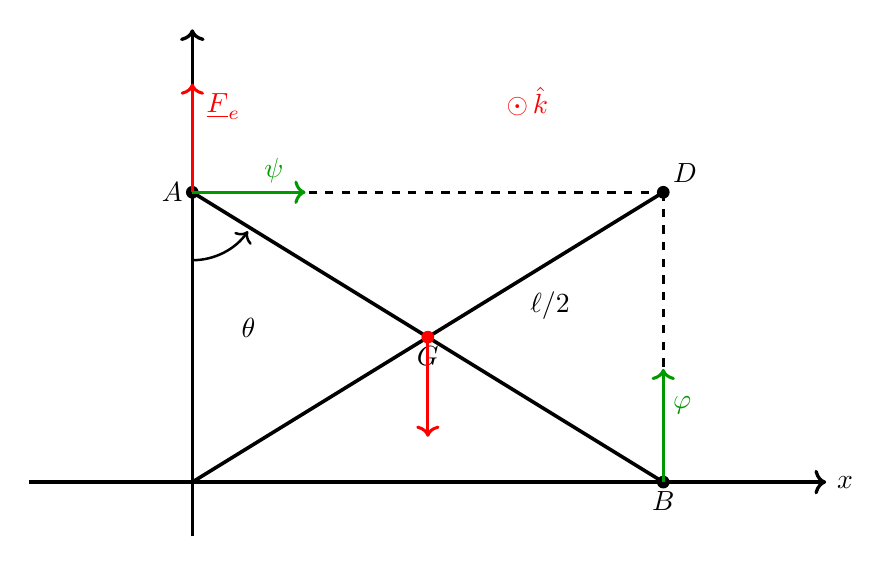
\begin{tikzpicture}[scale=1.15]
    % punti
    \coordinate (O) at (0,0);
    \coordinate (A) at (0,3.2);
    \coordinate (B) at (5.2,0);
    \coordinate (D) at (5.2,3.2);
    \coordinate (G) at ($(A)!0.5!(B)$);

    % assi
    \draw[->,line width=1.2pt] (-1.8,0) -- (7.0,0) node[right] {$x$};
    \draw[->,line width=1.2pt] (0,-0.6) -- (0,5.0);

    % asta e diagonale
    \draw[line width=1.3pt] (A) -- (B);
    \draw[line width=1.3pt] (O) -- (D);

    % tratteggi
    \draw[dashed,line width=1pt] (A) -- (D);
    \draw[dashed,line width=1pt] (D) -- (B);

    % punti
    \fill (A) circle (2pt);
    \fill (B) circle (2pt);
    \fill (D) circle (2pt);
    \fill[red] (G) circle (2pt);

    % etichette
    \node[left] at (A) {$A$};
    \node[below] at (B) {$B$};
    \node[above right] at (D) {$D$};
    \node[below] at (G) {$G$};

    % forza elastica
    \draw[->,red,line width=1.1pt] (A) -- ++(0,1.2);
    \node[red,right] at ($(A)+(0.05,0.95)$) {$\underline{F}_e$};

    % reazione psi in A
    \draw[->,green!60!black,line width=1.1pt] (A) -- ++(1.25,0);
    \node[green!60!black,above] at ($(A)+(0.9,0)$) {$\psi$};

    % reazione phi in B
    \draw[->,green!60!black,line width=1.1pt] (B) -- ++(0,1.25);
    \node[green!60!black,right] at ($(B)+(0,0.85)$) {$\varphi$};

    % peso in G
    \draw[->,red,line width=1.1pt] (G) -- ++(0,-1.1);

    % angolo theta
    \draw[->,line width=0.9pt] (0,2.45) arc[start angle=270,end angle=325,radius=0.75];
    \node at (0.62,1.7) {$\theta$};

    % scritta l/2
    \node at (3.95,1.95) {$\ell/2$};

    % versore k uscente
    \node[red] at (3.7,4.2) {$\odot\,\hat{k}$};
\end{tikzpicture}
\\Scriviamo la seconda equazione cardinale rispetto a \(D\):
\[
\frac{d}{dt}\Bigl((\underline{x}_G-\underline{x}_D)\wedge m\underline{v}_G
+I_G\underline{\omega}\Bigr)
=
(\underline{x}_B-\underline{x}_D)\wedge \varphi\,\hat{j}
+
(\underline{x}_A-\underline{x}_D)\wedge \psi\,\hat{i}
\]
\[
\qquad
+
(\underline{x}_A-\underline{x}_D)\wedge K\ell(1-\cos\theta)\,\hat{j}
+
(\underline{x}_G-\underline{x}_D)\wedge (-mg\,\hat{j})
-
\underline{v}_D\wedge m\underline{v}_G.
\]

Utilizziamo
\[
\underline{v}_G=\underline{\omega}\wedge(\underline{x}_G-\underline{x}_D)
\]
nel primo membro:
\[
\frac{d}{dt}\Bigl((\underline{x}_G-\underline{x}_D)\wedge
m\bigl(\underline{\omega}\wedge(\underline{x}_G-\underline{x}_D)\bigr)
+I_G\underline{\omega}\Bigr)
=
\frac{d}{dt}\Bigl(m\|\underline{x}_G-\underline{x}_D\|^{2}\underline{\omega}
+I_G\underline{\omega}\Bigr).
\]

Quindi
\[
\frac{d}{dt}\Bigl[\bigl(I_G+m\|\underline{x}_G-\underline{x}_D\|^{2}\bigr)
\dot{\theta}\,\hat{k}\Bigr]
=
\frac{d}{dt}\Bigl[\left(\frac{m\ell^{2}}{12}+m\left(\frac{\ell}{2}\right)^{2}\right)
\dot{\theta}\,\hat{k}\Bigr]
\]
\[
=
-\,\ell\sin\theta\cdot K\ell(1-\cos\theta)\,\hat{k}
+
\frac{\ell}{2}mg\sin\theta\,\hat{k}.
\]

Pertanto
\[
\frac{m\ell^{2}}{3}\,\ddot{\theta}
=
-\,K\ell^{2}\sin\theta(1-\cos\theta)
+
\frac{\ell}{2}mg\sin\theta.
\]

Questa equazione non si può risolvere analiticamente ma va risolta in modo
numerico.
\end{example}

\chapter{Statica del corpo rigido e moti per inerzia}
\section{Statica}

L'obiettivo della statica è trovare le \textbf{configurazioni di equilibrio di un sistema}.
Le configurazioni d'equilibrio sono caratterizzate dalle condizioni
\[
\underline{v}_G = 0,
\qquad
\underline{\omega} = 0,
\qquad
\begin{cases}
\displaystyle \sum_{i=1}^{n} \underline{f}_i^{\mathrm{ext}} = 0, \\[1ex]
\displaystyle \sum_{i=1}^{n} \underline{x}_i \wedge \underline{f}_i^{\mathrm{ext}} = 0.
\end{cases}
\]

\begin{example}{}
Studiamo la statica del seguente sistema

\begin{figure}
\centering
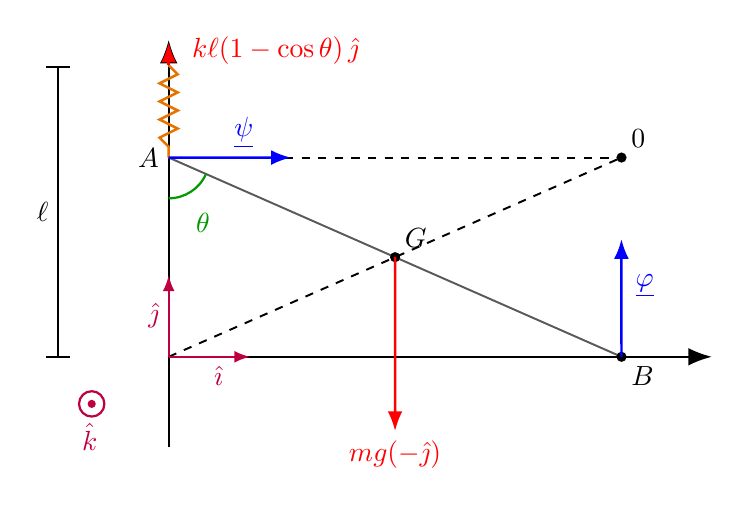
\begin{tikzpicture}[scale=1.15]
  % assi
  \draw[-{Latex[length=3mm]}, line width=0.8pt] (-0.2,-1.0) -- (-0.2,3.5);
  \draw[-{Latex[length=3mm]}, line width=0.8pt] (-0.2,0) -- (5.8,0);

  % punti principali
  \coordinate (A) at (-0.2,2.2);
  \coordinate (O) at (4.8,2.2);
  \coordinate (B) at (4.8,0);
  \coordinate (P) at (-0.2,0);
  \coordinate (G) at (2.3,1.1);

  % segmenti del sistema
  \draw[dashed, line width=0.7pt] (A) -- (O);
  \draw[dashed, line width=0.7pt] (P) -- (O);
  \draw[line width=0.7pt, gray!70!black] (A) -- (B);

  % punti
  \fill (O) circle (1.6pt);
  \fill (B) circle (1.6pt);
  \fill (G) circle (1.6pt);

  % etichette punti
  \node[left] at (A) {$A$};
  \node[above right] at (O) {$0$};
  \node[below right] at (B) {$B$};
  \node[above right] at (G) {$G$};

  % molla
  \draw[orange!90!black, line width=0.9pt]
    (-0.2,2.2) -- (-0.2,2.32)
    -- (-0.30,2.42) -- (-0.10,2.52)
    -- (-0.30,2.62) -- (-0.10,2.72)
    -- (-0.30,2.82) -- (-0.10,2.92)
    -- (-0.30,3.02) -- (-0.10,3.12)
    -- (-0.2,3.22);

  % forza elastica
  \draw[-{Latex[length=2.5mm]}, red, line width=0.9pt] (-0.2,3.22) -- (-0.2,3.47);
  \node[red, right] at (-0.05,3.38) {$k\ell(1-\cos\theta)\,\hat{\jmath}$};

  % psi
  \draw[-{Latex[length=2.5mm]}, blue, line width=0.9pt] (A) -- (1.15,2.2);
  \node[blue, above] at (0.63,2.2) {$\underline{\psi}$};

  % phi
  \draw[-{Latex[length=2.5mm]}, blue, line width=0.9pt] (B) -- (4.8,1.3);
  \node[blue, right] at (4.85,0.78) {$\underline{\varphi}$};

  % peso
  \draw[-{Latex[length=2.5mm]}, red, line width=0.9pt] (G) -- (2.3,-0.82);
  \node[red, below] at (2.3,-0.82) {$mg(-\hat{\jmath})$};

  % angolo theta
  \draw[green!60!black, line width=0.8pt] (-0.2,1.75) arc[start angle=-90,end angle=-24,radius=0.45];
  \node[green!60!black] at (0.18,1.48) {$\theta$};

  % triedro
  \draw[-{Latex[length=2mm]}, purple, line width=0.8pt] (-0.2,0) -- (0.7,0);
  \node[purple, below] at (0.35,0) {$\hat{\imath}$};

  \draw[-{Latex[length=2mm]}, purple, line width=0.8pt] (-0.2,0) -- (-0.2,0.9);
  \node[purple, left] at (-0.2,0.45) {$\hat{\jmath}$};

  \draw[purple, line width=0.8pt] (-1.05,-0.52) circle (0.14);
  \fill[purple] (-1.05,-0.52) circle (0.045);
  \node[purple, below left] at (-0.88,-0.63) {$\hat{k}$};

  % quota l
  \draw[line width=0.8pt] (-1.42,0) -- (-1.42,3.2);
  \draw[line width=0.8pt] (-1.55,0) -- (-1.29,0);
  \draw[line width=0.8pt] (-1.55,3.2) -- (-1.29,3.2);
  \node[left] at (-1.42,1.6) {$\ell$};
\end{tikzpicture}
\end{figure}

Imponiamo i vincoli della statica con polo $\underline{x}_0$ per i momenti
\[
\left\{
\begin{aligned}
\underline{\psi} + k\ell(1-\cos\theta)\,\hat{\jmath} + \underline{\varphi} - mg\,\hat{\jmath} &= 0 \\
(\underline{x}_A-\underline{x}_0)\wedge k\ell(1-\cos\theta)\,\hat{\jmath} + (\underline{x}_G-\underline{x}_0)\wedge -mg\,\hat{\jmath} &= 0
\end{aligned}
\right.
\qquad \Rightarrow \qquad
\]
\[
\Rightarrow
\left\{
\begin{aligned}
\psi &= 0 \\
k\ell(1-\cos\theta)+\varphi-mg &= 0 \\
(-\ell\sin\theta)\,k\ell(1-\cos\theta)\,\hat{k} + \frac{\ell}{2}mg\sin\theta\,\hat{k} &= 0
\end{aligned}
\right.
\]

\[
\Rightarrow
\left\{
\begin{aligned}
\psi &= 0 \\
k\ell(1-\cos\theta)+\varphi-mg &= 0 \\
-k\ell\sin\theta(1-\cos\theta)+\frac{mg}{2}\sin\theta &= 0
\end{aligned}
\right.
\]

Se pongo $\theta=\pi \wedge \theta\neq 0$ allora
\[
-k\ell(1-\cos\theta)+\frac{mg}{2}=0
\;\Rightarrow\;
k\ell\cos\theta=k\ell-\frac{mg}{2}
\;\Rightarrow\;
\cos\theta=1-\frac{mg}{2k\ell}
\]

Dal momento che \qquad $-1<\cos\theta<1$ \qquad allora
\[
-1<1-\frac{mg}{2k\ell}<1
\;\Leftrightarrow\;
-2<-\frac{mg}{2k\ell}<0
\;\Leftrightarrow\;
0<\frac{mg}{2k\ell}<2
\;\Leftrightarrow\;
0<mg<2k\ell
\;\Leftrightarrow\;
\frac{mg}{k\ell}<4
\]

Se $\dfrac{mg}{k\ell}<4$ la condizione \qquad $\cos\theta=1-\dfrac{mg}{2k\ell}$ \qquad dà 2 angoli \qquad $\theta_1,\theta_2$.

Una configurazione di equilibrio si ottiene anche per \qquad $\theta_3=0$ \quad e \quad $\theta_4=\pi$.

Notiamo che $\theta_3,\theta_4$ non sono vincolate a condizioni sui dati del sistema e quindi sono condizioni di equilibrio per ogni istanza del problema.

Notiamo infine che $\psi$ e $\varphi$ sono incognite e sono unicamente determinate da $\theta$.
\end{example}

\section{Moti per inerzia}

La condizione di staticità per il corpo rigido può essere considerata come un caso particolare di moto per inerzia. Diciamo che un corpo rigido si muove per inerzia se sussistono le condizioni
\[
\frac{d}{dt}\, m\underline{v_G} = 0
\qquad
\frac{d}{dt}\left(I_G \underline{\omega}\right) = 0
\]

\begin{example}{}
Consideriamo un sistema formato da un uomo seduto su una sedia che regge una ruota. Ipotizziamo che l'uomo faccia girare la ruota attorno ad un suo asse principale d'inerzia (asse di simmetria) con velocità angolare costante in modulo. Sia $G$ il centro di massa del sistema.

\begin{center}
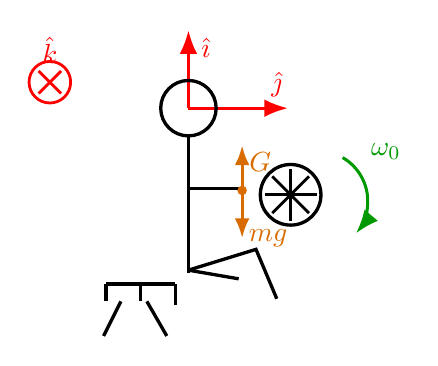
\begin{tikzpicture}[scale=1.1]
  % asse k uscente/entrante dal foglio
  \draw[red, line width=1pt] (-1.6,2.75) circle (0.24);
  \draw[red, line width=1pt] (-1.73,2.62)--(-1.47,2.88);
  \draw[red, line width=1pt] (-1.73,2.88)--(-1.47,2.62);
  \node[red] at (-1.6,3.12) {$\hat{k}$};

  % assi i e j
  \draw[red, -{Latex[length=3mm]}, line width=1.1pt] (0,2.45)--(0,3.35);
  \node[red] at (0.2,3.15) {$\hat{\imath}$};
  \draw[red, -{Latex[length=3mm]}, line width=1.1pt] (0,2.45)--(1.15,2.45);
  \node[red] at (1.02,2.72) {$\hat{\jmath}$};

  % uomo
  \draw[line width=1.2pt] (0,2.45) circle (0.32);
  \draw[line width=1.2pt] (0,2.13)--(0,0.55);
  \draw[line width=1.2pt] (0,1.52)--(0.62,1.52);
  \draw[line width=1.2pt] (0,0.58)--(0.78,0.82)--(1.02,0.25);
  \draw[line width=1.2pt] (0,0.58)--(0.58,0.48);
  \draw[line width=1.2pt] (-0.15,0.42)--(-0.15,0.18);
  \draw[line width=1.2pt] (-0.15,0.42)--(-0.55,0.42);
  \draw[line width=1.2pt] (-0.55,0.42)--(-0.55,0.22);
  \draw[line width=1.2pt] (-0.55,0.42)--(-0.95,0.42);
  \draw[line width=1.2pt] (-0.95,0.42)--(-0.95,0.22);
  \draw[line width=1.2pt] (-0.78,0.22)--(-0.98,-0.18);
  \draw[line width=1.2pt] (-0.48,0.22)--(-0.25,-0.18);

  % linea verticale arancione, G e mg
  \draw[orange!85!black, {Latex[length=2.5mm]}-{Latex[length=2.5mm]}, line width=1.1pt] (0.62,0.95)--(0.62,2.02);
  \fill[orange!85!black] (0.62,1.50) circle (0.055);
  \node[orange!85!black] at (0.83,1.83) {$G$};
  \node[orange!85!black] at (0.92,0.95) {$mg$};

  % ruota
  \draw[line width=1.2pt] (1.18,1.45) circle (0.35);
  \fill (1.18,1.45) circle (0.05);
  \foreach \a in {0,45,...,315}{
    \draw[line width=1pt] (1.18,1.45)--++(\a:0.3);
  }

  % freccia angolare
  \draw[green!60!black, -{Latex[length=3mm]}, line width=1.1pt]
    (1.78,1.88) arc[start angle=60,end angle=-40,radius=0.58];
  \node[green!60!black] at (2.28,1.95) {$\omega_0$};
\end{tikzpicture}
\end{center}

Dal momento che l'asse di rotazione è un asse principale d'inerzia allora
\[
I_G^{\text{ruota}}\underline{\omega}_0=\omega_0 I_G^{\text{ruota}}\hat{k}=\omega_0 I_G^{\text{ruota},zz}\hat{k}
\]

ovvero il momento angolare ha direzione $\hat{k}$. In particolare, a patto di continuare a effettuare la rotazione attorno ad un asse principale, il momento angolare ha stessa direzione della velocità angolare ad ogni istante $t$, anche se quest'ultima cambia direzione.

L'uomo è inizialmente fermo e quindi $\omega_1=0$ e $I_G^{\text{uomo}}\underline{\omega}_1=0$.

I momenti delle forze esterne al sistema in direzione $\hat{\imath}$ sono nulli e quindi il momento angolare totale in direzione $\hat{\imath}$ deve essere costante ovvero uguale a
\[
\left[\left(I_G^{\text{ruota}}\underline{\omega}_0+I_G^{\text{uomo}}\underline{\omega}_1\right)\cdot\hat{\imath}\right]\hat{\imath}=0
\]

Ad un istante $t>0$ l'uomo inclina la ruota di un angolo $\theta$ facendola girare sempre alla stessa velocità.

\begin{center}
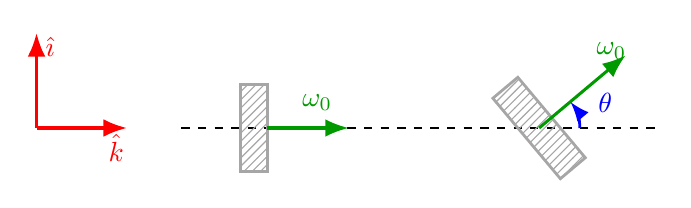
\begin{tikzpicture}[scale=1.15]
  % assi
  \draw[red, -{Latex[length=3mm]}, line width=1.1pt] (0,0)--(0,1.05);
  \node[red] at (0.15,0.9) {$\hat{\imath}$};
  \draw[red, -{Latex[length=3mm]}, line width=1.1pt] (0,0)--(1.0,0);
  \node[red] at (0.88,-0.22) {$\hat{k}$};

  % linea tratteggiata
  \draw[dashed, line width=1pt] (1.6,0)--(6.9,0);

  % ruota iniziale
  \draw[gray!70, line width=1pt, pattern=north east lines, pattern color=gray!70]
    (2.25,-0.48) rectangle (2.55,0.48);
  \draw[green!60!black, -{Latex[length=3mm]}, line width=1.1pt] (2.55,0)--(3.45,0);
  \node[green!60!black] at (3.1,0.28) {$\omega_0$};

  % ruota inclinata
  \begin{scope}[shift={(5.55,0)}, rotate=40]
    \draw[gray!70, line width=1pt, pattern=north east lines, pattern color=gray!70]
      (-0.18,-0.58) rectangle (0.18,0.58);
  \end{scope}

  % nuova velocità angolare
  \draw[green!60!black, -{Latex[length=3mm]}, line width=1.1pt] (5.55,0)--++(40:1.25);
  \node[green!60!black] at (6.35,0.85) {$\omega_0$};

  % angolo theta
  \draw[blue, -{Latex[length=2.5mm]}, line width=1pt] (6.0,0) arc[start angle=0,end angle=40,radius=0.45];
  \node[blue] at (6.28,0.28) {$\theta$};
\end{tikzpicture}
\end{center}

Allora
\[
I_G^{\text{ruota}}\underline{\omega}_0=\omega_0 I_G^{\text{ruota},zz}\cos\theta\,\hat{k}+\omega_0 I_G^{\text{ruota},zz}\sin\theta\,\hat{\imath}
\]

Per quanto detto prima il momento angolare totale lungo $\hat{\imath}$ deve rimanere nullo ovvero
\[
I_G^{\text{ruota},zz}\omega_0\sin\theta+I_G^{\text{uomo},xx}\omega_1=0
\qquad\Rightarrow\qquad
\omega_1=-\frac{I_G^{\text{ruota},zz}\omega_0\sin\theta}{I_G^{\text{uomo},xx}}
\]

L'uomo inizia quindi a girare in senso orario.

\end{example}

\begin{example}{}
Per lo stesso motivo dell'esempio precedente un pattinatore allarga le gambe e braccia per rallentare e le chiude per andare più veloce. Infatti
\[
I_G^1 \omega_1 = I_G^2 \omega_2
\]
con
\[
I_G^1 > I_G^2 \Rightarrow \omega_2 > \omega_1
\]
\end{example}

Analizziamo meglio i vincoli del moto per inerzia.
\[
\frac{d}{dt}\left(m\underline{v}_G\right)=0 \Leftrightarrow m\frac{d}{dt}\underline{v}_G=0
\Rightarrow
\left\{
\begin{aligned}
m\frac{d}{dt}v_G^x &= 0\\
m\frac{d}{dt}v_G^y &= 0\\
m\frac{d}{dt}v_G^z &= 0
\end{aligned}
\right.
\Rightarrow
\left\{
\begin{aligned}
v_G^x &= C_x \in \mathbb{R}\\
v_G^y &= C_y \in \mathbb{R}\\
v_G^z &= C_z \in \mathbb{R}
\end{aligned}
\right.
\Rightarrow
\underline{v}_G(t)=\underline{v}_G(0)\qquad \forall\ t
\]

Lo stesso non si può fare con il secondo infatti
\[
\frac{d}{dt}\left(I_G\omega\right)=0 \not\Rightarrow I_G\frac{d}{dt}(\omega)=0
\]

dal momento che $I_G$ è in realtà una funzione del tempo perché questa dipende dalla distribuzione delle masse dato un orientamento del corpo rigido.

Ad esempio
\[
I_G^{11}=\sum_{i=1}^{n}m_i\left(y_i^2+z_i^2\right)
\]
dipende dall'orientamento del corpo rigido rispetto al sistema di assi coordinati.

La soluzione è quella di usare un sistema di assi coordinati mobili solidali al corpo così che la matrice d'inerzia sia costante.

Al tempo $t=0$ scelgo gli assi $\hat{\imath}(t),\hat{\jmath}(t),\hat{k}(t)$ orientati come gli assi principali d'inerzia. Così possiamo scrivere per ogni istante $t$
\[
I_G=
\begin{pmatrix}
I_G^{xx} & 0 & 0\\
0 & I_G^{yy} & 0\\
0 & 0 & I_G^{zz}
\end{pmatrix}
\qquad
\omega=
\begin{pmatrix}
\omega_x\\
\omega_y\\
\omega_z
\end{pmatrix}
\qquad \Rightarrow \qquad
I_G\omega = I_G^{xx}\omega_x\,\hat{\imath}(t)+I_G^{yy}\omega_y\,\hat{\jmath}(t)+I_G^{zz}\omega_z\,\hat{k}(t)
\]

Prima di andare avanti ci serve la seguente.

\begin{lemma}{}[Formula di Poisson]
Sia $O$ un punto di un corpo rigido e sia $\{O,\underline{e}_1,\underline{e}_2,\underline{e}_3\}$ un qualsiasi riferimento ortonormale solidale al corpo rigido. Allora $\forall i=1,\ldots,3$ vale
\[
\dot{\underline{e}}_i=\underline{\omega}\wedge\underline{e}_i
\]
\end{lemma}
\inizioapprof
\begin{proof}
Consideriamo $\{O,\underline{e}_1,\underline{e}_2,\underline{e}_3\}$ e un punto $P$ del corpo tale che
\[
\underline{x}_P-\underline{x}_O=\underline{e}_i
\]
Allora vale
\[
\underline{v}_P=\underline{v}_O+\underline{\omega}\wedge\underline{e}_i
\qquad\Rightarrow\qquad
\underline{v}_P-\underline{v}_O=\underline{\omega}\wedge\underline{e}_i
\]
Ma
\[
\frac{d}{dt}\,\underline{e}_i=\frac{d}{dt}\left(\underline{x}_P-\underline{x}_O\right)=\underline{v}_P-\underline{v}_O
\]
allora
\[
\dot{\underline{e}}_i=\underline{\omega}\wedge\underline{e}_i \quad \forall i = 1 , \ldots , 3.
\]


\end{proof}
\fineapprof
Riscriviamo il vincolo
\[
\frac{d}{dt}\left(I_G\underline{\omega}\right)=
\frac{d}{dt}\left(I_G^{xx}\omega_x\hat{\imath}(t)+I_G^{yy}\omega_y\hat{\jmath}(t)+I_G^{zz}\omega_z\hat{k}(t)\right)=
\]
\[
= I_G^{xx}\dot{\omega}_x\hat{\imath}
+ I_G^{xx}\omega_x\frac{d\hat{\imath}}{dt}
+ I_G^{yy}\dot{\omega}_y\hat{\jmath}
+ I_G^{yy}\omega_y\frac{d\hat{\jmath}}{dt}
+ I_G^{zz}\dot{\omega}_z\hat{k}
+ I_G^{zz}\omega_z\frac{d\hat{k}}{dt}
=0
\]

Per la formula di Poisson si ha che
\[
\frac{d\hat{\imath}}{dt}=\underline{\omega}\wedge\hat{\imath}
\qquad
\frac{d\hat{\jmath}}{dt}=\underline{\omega}\wedge\hat{\jmath}
\qquad
\frac{d\hat{k}}{dt}=\underline{\omega}\wedge\hat{k}
\]

Semplifichiamo la notazione : \quad $I_G^{xx}=I_1 \qquad I_G^{yy}=I_2 \qquad I_G^{zz}=I_3$

\[
\Rightarrow\quad
I_1\dot{\omega}_x\hat{\imath}
+I_1\omega_x(\underline{\omega}\wedge\hat{\imath})
+I_2\dot{\omega}_y\hat{\jmath}
+I_2\omega_y(\underline{\omega}\wedge\hat{\jmath})
+I_3\dot{\omega}_z\hat{k}
+I_3\omega_y(\underline{\omega}\wedge\hat{k})
=0
\]

e dal momento che
\[
\underline{\omega}\wedge\hat{\imath}
=
\begin{vmatrix}
\hat{\imath} & \hat{\jmath} & \hat{k}\\
\omega_x & \omega_y & \omega_z\\
1 & 0 & 0
\end{vmatrix}
= \omega_z\hat{\jmath}-\omega_y\hat{k}
\qquad
\underline{\omega}\wedge\hat{\jmath}
=
\begin{vmatrix}
\hat{\imath} & \hat{\jmath} & \hat{k}\\
\omega_x & \omega_y & \omega_z\\
0 & 1 & 0
\end{vmatrix}
= -\omega_z\hat{\imath}+\omega_x\hat{k}
\]
\[
\underline{\omega}\wedge\hat{k}
=
\begin{vmatrix}
\hat{\imath} & \hat{\jmath} & \hat{k}\\
\omega_x & \omega_y & \omega_z\\
0 & 0 & 1
\end{vmatrix}
= \omega_y\hat{\imath}-\omega_x\hat{\jmath}
\]

\[
\Rightarrow\quad
I_1\dot{\omega}_x\hat{\imath}
+I_1\omega_x(\omega_z\hat{\jmath}-\omega_y\hat{k})
+I_2\dot{\omega}_y\hat{\jmath}
+I_2\omega_y(-\omega_z\hat{\imath}+\omega_x\hat{k})
+I_3\dot{\omega}_z\hat{k}
+
+I_3\omega_z(\omega_y\hat{\imath}-\omega_x\hat{\jmath})
=0
\]

\[
\Rightarrow
\left\{
\begin{aligned}
I_1\dot{\omega}_x - I_2\omega_y\omega_z + I_3\omega_y\omega_z &= 0\\
I_2\dot{\omega}_y + I_1\omega_x\omega_z - I_3\omega_x\omega_z &= 0\\
I_3\dot{\omega}_z - I_1\omega_x\omega_y + I_2\omega_x\omega_y &= 0
\end{aligned}
\right.
\qquad \Rightarrow \qquad
\left\{
\begin{aligned}
\dot{\omega}_x &= \omega_y\omega_z\,\frac{I_2-I_3}{I_1}\\
\dot{\omega}_y &= \omega_x\omega_z\,\frac{I_3-I_1}{I_2}\\
\dot{\omega}_z &= \omega_x\omega_y\,\frac{I_1-I_2}{I_3}
\end{aligned}
\right.
\]

Abbiamo ottenuto quelle che chiamiamo \textbf{equazioni del moto per inerzia di un corpo rigido}.\\
 Queste sono 3 equazioni differenziali accoppiate che in generale si risolvono numericamente. Il problema si può risolvere analiticamente quando un corpo ha un asse di simmetria, ovvero quando $I_1=I_2=I$. Allora il sistema diventa
\[
\left\{
\begin{aligned}
\dot{\omega}_x &= \omega_0\omega_y\,\frac{I-I_3}{I}\\[4pt]
\dot{\omega}_y &= \omega_0\omega_x\,\frac{I_3-I}{I}\\[4pt]
\dot{\omega}_z &= 0 \qquad \Rightarrow \qquad \omega_z=\omega_0
\end{aligned}
\right.
\]

Vogliamo arrivare ad un'equazione disaccoppiata
\[
\ddot{\omega}_x=\omega_0\dot{\omega}_y\,\frac{I-I_3}{I}
=\omega_0\omega_0\omega_x\,\frac{I_3-I}{I}\cdot\frac{I-I_3}{I}
=-\omega_0^2\left(\frac{I-I_3}{I}\right)^2\omega_x
\]

L'equazione è quella di un oscillatore armonico semplice e posto
\[
\Omega=\omega_0\frac{I-I_3}{I}
\]
ha soluzione
\[
\omega_x(t)=A\cos(\Omega t+\psi)
\qquad \Rightarrow \qquad
\dot{\omega}_y(t)=\omega_0A\cos(\Omega t+\psi)\frac{I_3-I}{I}
\qquad \Rightarrow
\]
\[
\Rightarrow \qquad
\omega_y(t)=A\sin(\Omega t+\psi)\cdot \omega_0\cdot\frac{I_3-I}{I}\cdot\frac{1}{\Omega}
= A\sin(\Omega t+\psi)
\]

ovvero detto $\omega_z=\omega_0$
\[
\left\{
\begin{aligned}
\omega_x &= A\cos(\Omega t+\psi)\\
\omega_y &= A\sin(\Omega t+\psi)
\end{aligned}
\right.
\]

Notiamo che se consideriamo $\{O , \hat{i'} , \hat{j'} , \hat{k'}\}$ sistema di riferimento fisso e accoppiamo le equazioni e le condizioni
\[
\left\{
\begin{aligned}
\dot{\omega}_x &= \omega_y\omega_z\,\frac{I_2-I_3}{I_1} , \quad  \dot{\omega}_y = \omega_x\omega_z\,\frac{I_3-I_1}{I_2}, \quad \dot{\omega}_z = \omega_x\omega_y\,\frac{I_1-I_2}{I_3}\\
& \underline{\omega}(0) = (\omega_{x0} , \omega_{y0} , \omega_{z0}),\\
\hat{\dot{i}} &= \underline{\omega} \wedge \hat{i}, \quad  \hat{\dot{j}} = \underline{\omega} \wedge \hat{j}, \quad  \hat{\dot{k}} = \underline{\omega} \wedge \hat{k}\\
\hat{i} (0) &= i_{x'0} \hat{i'} + i_{y'0} \hat{j'} + i_{z'0} \hat{k'} \\
\hat{j} (0) &= j_{x'0} \hat{i'} + j_{y'0} \hat{j'} + j_{z'0} \hat{k'} \\
\hat{k} (0) &= k_{x'0} \hat{i'} + k_{y'0} \hat{j'} + k_{z'0} \hat{k'}\\
\underline{v}_G(t) &= \underline{v}_G(0) \quad \forall t
\end{aligned}
\right.
\]
otteniamo una descrizione completa del moto.

\subsection{Stabilità del moto per inerzia di un corpo rigido}
Un'altra condizione che rende risolvibile il sistema in modo analitico è la condizione iniziale
\[
\underline{\omega}(0)=(0,0,\omega_0)
\qquad
\text{(oppure } \underline{\omega}(0)=(\omega_0,0,0),\ \underline{\omega}(0)=(0,\omega_0,0)\text{).}
\]
Vogliamo quindi risolvere il problema di Cauchy
\[
\left\{
\begin{aligned}
\dot{\omega}_x &= \omega_y\omega_z\cdot \frac{I_y-I_z}{I_x} \\
\dot{\omega}_y &= \omega_x\omega_z\cdot \frac{I_z-I_x}{I_y} \\
\dot{\omega}_z &= \omega_x\omega_y\cdot \frac{I_x-I_y}{I_z} \\
\underline{\omega}(0) &= (0,0,\omega_0)
\end{aligned}
\right.
\]

Consideriamo la possibile soluzione
\[
\underline{\omega}(t)=(0,0,\omega_0).
\]
Notiamo che soddisfa il problema di Cauchy infatti
\[
\underline{\omega}(0)=(0,0,\omega_0)
\]
\[
\dot{\omega}_x(t)=0=\omega_y(t)\cdot\omega_z(t)\cdot\frac{I_y-I_z}{I_x}
=0\cdot\omega_0\cdot\frac{I_y-I_z}{I_x}=0
\]
\[
\dot{\omega}_y(t)=0=\omega_x(t)\cdot\omega_z(t)\cdot\frac{I_z-I_x}{I_y}
=0\cdot\omega_0\cdot\frac{I_z-I_x}{I_y}=0
\]
\[
\dot{\omega}_z(t)=0=\omega_x(t)\cdot\omega_y(t)\cdot\frac{I_x-I_y}{I_z}
=0\cdot 0\cdot\frac{I_x-I_y}{I_z}=0
\]

Per l'unicità della soluzione di un problema di Cauchy allora
\[
\underline{\omega}(t)=(0,0,\omega_0)
\]
è l'unica possibile soluzione.


Imponendo quindi la velocità angolare iniziale lungo un asse principale d'inerzia si ottiene un moto semplice da descrivere.
Nella realtà imporre questo tipo di condizione è molto difficile. Vogliamo studiare quindi come piccole perturbazioni della condizione iniziale influenzino la soluzione del sistema. Per fare ciò introduciamo in maniera non rigorosa il concetto di stabilità. Ritorneremo su una trattazione di stabilità più rigorosa nelle prossime lezioni.

\begin{definition}{}
Diciamo che $\underline{\omega}^{*}(t)=(0,0,\omega_0)$ è stabile se assegnando condizioni iniziali ``vicine'' a $\underline{\omega}(0)=(0,0,\omega_0)$ otteniamo una soluzione $\underline{\omega}(t)$ ``vicina'' a $\underline{\omega}^{*}(t)$.
\end{definition}

Per studiare se la soluzione è stabile, consideriamo una condizione iniziale perturbata
\[
\underline{\omega}(0)=(\omega_x^0,\omega_y^0,\omega_0)
\qquad \text{con} \qquad
|\omega_y^0|,\,|\omega_x^0| \ll |\omega_0|.
\]

Scriviamo le equazioni per il problema perturbato nei primi istanti del moto. Suppongo che
\[
\left\{
\begin{aligned}
\omega_x(t) &= \omega'_x(t) \\
\omega_y(t) &= \omega'_y(t) \\
\omega_z(t) &= \omega_0 + \omega'_z(t)
\end{aligned}
\right.
\]

Sostituendo nel sistema si ottiene
\[
\left\{
\begin{aligned}
\dot{\omega}'_x &= \omega'_y(\omega_0+\omega'_z)\,\frac{I_y-I_z}{I_x} \\
\dot{\omega}'_y &= (\omega_0+\omega'_z)\omega_x\,\frac{I_z-I_x}{I_y} \\
\dot{\omega}'_z &= \omega'_x\omega'_y\,\frac{I_x-I_y}{I_z}
\end{aligned}
\right.
\]

Dal momento che stiamo supponendo tutte le funzioni continue per un $t$ sufficientemente piccolo possiamo dire che
\[
|\omega'_x(t)| \ll |\omega_0|,
\qquad
|\omega'_y(t)| \ll |\omega_0|
\]
allora trascuriamo i termini che non contengono $\omega_0$
\[
\left\{
\begin{aligned}
\dot{\omega}'_x &= \omega'_y\,\omega_0\,\frac{I_y-I_z}{I_x} \\
\dot{\omega}'_y &= \omega_0\,\omega'_x\,\frac{I_z-I_x}{I_y} \\
\dot{\omega}'_z &= 0
\end{aligned}
\right.
\]


Derivo la prima equazione e sostituisco la seconda
\[
\ddot{\omega}'_x
=
\dot{\omega}'_y\,\omega_0\,\frac{I_y-I_z}{I_x}
=
\omega_0\,\omega'_x\cdot\frac{I_z-I_x}{I_y}\cdot\omega_0\,\frac{I_y-I_z}{I_x}
=
\frac{\omega_0^2}{I_xI_y}(I_z-I_x)(I_y-I_z)\,\omega'_x
\]

Se
\[
a=(I_z-I_x)(I_y-I_z)<0
\]
allora ho l'equazione dell'oscillatore armonico. In questo caso quindi la perturbazione è limitata dai dati iniziali e quindi possiamo dire che $\underline{\omega}(t)$ è stabile.

Se $a>0$ abbiamo una crescita esponenziale nella perturbazione e quindi possiamo dire che $\underline{\omega}(t)$ è instabile.

\begin{itemize}
    \item $a<0$ se $I_z$ è il più piccolo o il più grande tra i momenti d'inerzia.
    \item $a>0$ se $I_z$ è intermedio tra gli altri due.
\end{itemize}


\section{Il problema del gommista}
Supponiamo di avere una ruota vincolata a ruotare attorno ad un asse che non è principale d'inerzia. Denotiamo il versore dell'asse principale d'inerzia con \(\hat{k}'\) e con \(\underline{\omega}\) la velocità angolare della ruota. L'asse di rotazione è fisso e \(\underline{\omega}\) costante, tale che \(\underline{\omega} \wedge \hat{k}' \neq \underline{0}\).\\

\begin{center}
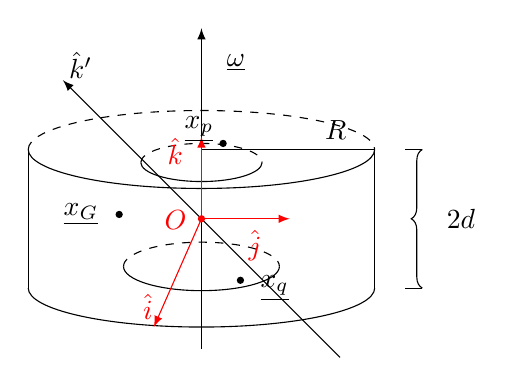
\begin{tikzpicture}[scale=1.1, >=latex]

% cilindro
\draw (-2,0.8) arc[start angle=180,end angle=360,x radius=2,y radius=0.45];
\draw (-2,-0.8) arc[start angle=180,end angle=360,x radius=2,y radius=0.45];
\draw (-2,0.8) -- (-2,-0.8);
\draw (2,0.8) -- (2,-0.8);
\draw[dashed] (-2,0.8) arc[start angle=180,end angle=0,x radius=2,y radius=0.45];

% ellissi interne
\draw (-0.7,0.65) arc[start angle=180,end angle=360,x radius=0.7,y radius=0.22];
\draw[dashed] (-0.7,0.65) arc[start angle=180,end angle=0,x radius=0.7,y radius=0.22];

\draw (-0.9,-0.55) arc[start angle=180,end angle=360,x radius=0.9,y radius=0.28];
\draw[dashed] (-0.9,-0.55) arc[start angle=180,end angle=0,x radius=0.9,y radius=0.28];

% asse verticale e omega
\draw[->] (0,-1.5) -- (0,2.2);
\node[right] at (0.18,1.8) {\(\underline{\omega}\)};

% asse inclinato
\draw[->] (1.6,-1.6) -- (-1.6,1.6);
\node[left] at (-1.15,1.77) {\(\hat{k}'\)};

% raggio orizzontale dell'ellisse esterna superiore
\draw (0,0.8) -- (2,0.8);
\node[above] at (1.55,0.8) {\(R\)};

% sistema di riferimento rosso con origine all'intersezione degli assi
\fill[red] (0,0) circle (1.2pt);
\node[red,left] at (-0.06,-0.02) {\(O\)};

\draw[->,red] (0,0) -- (0,0.95);
\node[red,left] at (-0.1,0.78) {\(\hat{k}\)};

\draw[->,red] (0,0) -- (-0.55,-1.25);
\node[red,left] at (-0.45,-1.02) {\(\hat{i}\)};

\draw[->,red] (0,0) -- (1.02,0);
\node[red,below] at (0.62,-0.02) {\(\hat{j}\)};

% punti e label
\fill (-0.95,0.05) circle (1.2pt);
\node[left] at (-1.08,0.05) {\(\underline{x_G}\)};

\fill (0.25,0.87) circle (1.2pt);
\node[left] at (0.25,1.03) {\(\underline{x_p}\)};

\fill (0.45,-0.71) circle (1.2pt);
\node[right] at (0.57,-0.8) {\(\underline{x_q}\)};

% quota 2d
\draw (2.35,0.8) -- (2.55,0.8);
\draw (2.35,-0.8) -- (2.55,-0.8);
\draw[decorate,decoration={brace,mirror,amplitude=4pt}] (2.55,0.8) -- (2.55,-0.8);
\node[right] at (2.72,0) {\(2d\)};

\end{tikzpicture}
\end{center}

Centriamo un sistema di riferimento \(\{O,\hat{i},\hat{j},\hat{k}\}\) al centro della ruota così che la ruota si estenda lungo \(\hat{k}\) da \(-d\) a \(d\).\\
Supponiamo inoltre che \(\underline{x_G}\) non passi per la direzione di \(\underline{\omega}\) perché la ruota ha subito deformazioni.\\
L'asse fisso impone i vincoli \(\omega_x=\omega_y=0\) a cui corrispondono le reazioni vincolari di momento \(\underline{M}=M_x\hat{\imath}+M_y\hat{\jmath}\). L'idea è che se la ruota è vincolata a ruotare attorno ad un asse che non è principale d'inerzia il momento angolare deve necessariamente variare nel tempo per permettere la rotazione. Abbiamo visto nella scorsa lezione infatti che l'unico modo per cui questo non accada è che l'asse sia principale d'inerzia. Impostiamo la seconda legge cardinale

\[
\frac{d}{dt}\left(I_G\underline{\omega}\right)=\underline{M}
\;\Rightarrow\;
\frac{d}{dt}\left[
\begin{pmatrix}
I_{xx} & I_{xy} & I_{xz} \\
I_{yx} & I_{yy} & I_{yz} \\
I_{zx} & I_{zy} & I_{zz}
\end{pmatrix}
\begin{pmatrix}
0 \\
0 \\
\omega
\end{pmatrix}
\right]
=
\begin{pmatrix}
M_x \\
M_y \\
0
\end{pmatrix}
\;\Rightarrow
\]

\[
\Rightarrow
\begin{cases}
\dfrac{d}{dt}\left(I_{xz}\,\omega\right)=M_x \\[1ex]
\dfrac{d}{dt}\left(I_{yz}\,\omega\right)=M_y
\end{cases}
\]
Qui quello che varia sono proprio $I_{xz}, I_{yz}$ perché il corpo gira attorno ad un sistema di assi non solidali e rispetto al quale non è simmetrico. Vogliamo quindi spostare gli assi principali d'inerzia così che quei momenti d'inerzia siano costanti e uguali a 0.\\
Per fare ciò il gommista deve aggiungere delle masse sul cerchione in modo tale che

\begin{itemize}
\item \(I_{xz}=I_{yz}=0\)
\item \(x_G=y_G=0\)
\end{itemize}

così che \(\hat{k}\) diventi asse principale d'inerzia e che \(M_x=M_y=0\).

Ricordiamo che
\[
I_{xz}=-\sum_i m_i\,x_i\,z_i
\]

\[
I_{yz}=-\sum_i m_i\,y_i\,z_i
\]


Per allineare l'asse principale d'inerzia con \(\underline{\omega}\) sommiamo al sistema 2 masse \(m_p,m_q\) di posizione \(\underline{x_q},\underline{x_p}\).

Per ragioni fisiche vogliamo mettere una massa sul bordo del cerchione superiore e una sul bordo del cerchione inferiore.

\begin{center}
\begin{minipage}{0.45\textwidth}
\centering
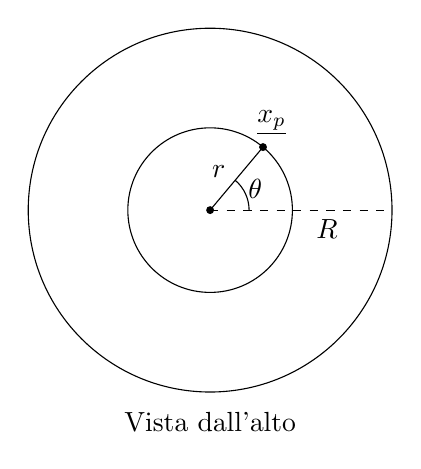
\begin{tikzpicture}[scale=1.1,>=latex]
\draw (0,0) circle (2.1);
\draw (0,0) circle (0.95);

\fill (0,0) circle (1.3pt);
\coordinate (P) at ({0.95*cos(50)},{0.95*sin(50)});
\fill (P) circle (1.3pt);

\draw (0,0) -- (P);
\draw[dashed] (0,0) -- (2.1,0);

\draw (0.45,0) arc[start angle=0,end angle=50,radius=0.45];

\node at (0.1,0.45) {\(r\)};
\node at (0.52,0.24) {\(\theta\)};
\node at (1.35,-0.22) {\(R\)};
\node at ($(P)+(0.1,0.28)$) {\(\underline{x_p}\)};

\node at (0,-2.45) {Vista dall'alto};
\end{tikzpicture}
\end{minipage}
\hfill
\begin{minipage}{0.45\textwidth}
\centering
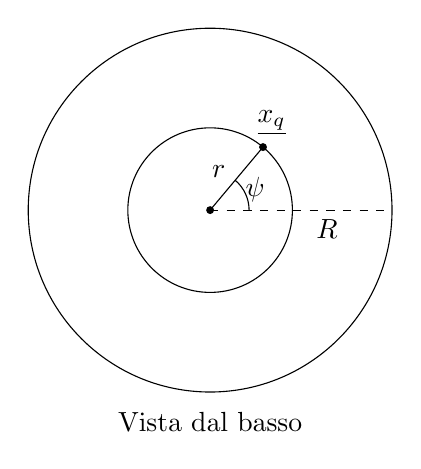
\begin{tikzpicture}[scale=1.1,>=latex]
\draw (0,0) circle (2.1);
\draw (0,0) circle (0.95);

\fill (0,0) circle (1.3pt);
\coordinate (Q) at ({0.95*cos(50)},{0.95*sin(50)});
\fill (Q) circle (1.3pt);

\draw (0,0) -- (Q);
\draw[dashed] (0,0) -- (2.1,0);

\draw (0.45,0) arc[start angle=0,end angle=50,radius=0.45];

\node at (0.1,0.45) {\(r\)};
\node at (0.52,0.24) {\(\psi\)};
\node at (1.35,-0.22) {\(R\)};
\node at ($(Q)+(0.1,0.28)$) {\(\underline{x_q}\)};

\node at (0,-2.45) {Vista dal basso};
\end{tikzpicture}
\end{minipage}
\end{center}
Impongo quindi \(\underline{x_p}=(r\cos\theta,r\sin\theta,d)\), \(\underline{x_q}=(r\cos\varphi,r\sin\varphi,-d)\).

Scriviamo nel caso generale le condizioni

\[
\text{1) il centro di massa è sull'asse } \hat{k}
\]

\[
\text{2) } \hat{k} \text{ asse principale d'inerzia}
\]

\[
\left\{
\begin{aligned}
m\,x_G + m_p\,x_p + m_q\,x_q &= 0\\
m\,y_G + m_p\,y_p + m_q\,y_q &= 0\\
I_{xz} - m_p\,x_p\,z_p - m_q\,x_q\,z_q &= 0\\
I_{yz} - m_p\,y_p\,z_p - m_q\,y_q\,z_q &= 0
\end{aligned}
\right.
\]

Il sistema è nelle 8 incognite \(m_p,m_q,x_p,x_q,y_p,y_q,z_p,z_q\).
Applicando la restrizione per \(\underline{x_p}\) e \(\underline{x_q}\) possiamo ridurre le incognite alle 4 \(\theta,\varphi,m_p,m_q\).

\[
\left\{
\begin{aligned}
m_p\,r\cos\theta + m_q\,r\cos\varphi &= -m\,x_G \qquad \text{(I)}\\
m_p\,r\sin\theta + m_q\,r\sin\varphi &= -m\,y_G \qquad \text{(II)}\\
m_p\,d r\cos\theta - m_q\,d r\cos\varphi &= I_{xz} \qquad \text{(III)}\\
m_p\,d r\sin\theta - m_q\,d r\sin\varphi &= I_{yz} \qquad \text{(IV)}
\end{aligned}
\right.
\]

La soluzione è

\[
m_p=\frac{1}{2r}\sqrt{\left(-m x_G+\frac{I_{xz}}{d}\right)^2+\left(-m y_G+\frac{I_{yz}}{d}\right)^2}
\]

\[
m_q=\frac{1}{2r}\sqrt{\left(-m x_G-\frac{I_{xz}}{d}\right)^2+\left(-m y_G-\frac{I_{yz}}{d}\right)^2}
\]

\[
\theta=\operatorname{atan2}\left(-m y_G+\frac{I_{yz}}{d},-m x_G+\frac{I_{xz}}{d}\right)
\]

\[
\varphi=\operatorname{atan2}\left(-m y_G-\frac{I_{yz}}{d},-m x_G-\frac{I_{xz}}{d}\right)
\]

\chapter{Teorema di König ed energia cinetica}
\begin{definition}{}
Sia \(\underline{v}=\dot{\underline{x}}\) la velocità di un punto materiale di massa \(m\). Definiamo energia cinetica del punto la quantità
\[
T=m\frac{\underline{v}\cdot\underline{v}}{2}=m\frac{v^2}{2}
\]
Per un sistema di punti ciascuno di velocità \(\underline{v_i}\) e massa \(m_i\) si dice energia cinetica del sistema la quantità
\[
T=\sum_{i=1}^{n} m_i\cdot\frac{v_i^2}{2}
\]
\end{definition}
Prima di enunciare e dimostrare il teorema di König abbiamo bisogno del seguente lemma

\begin{lemma}{}
Siano \(\underline{a},\underline{b},\underline{c}\in\mathbb{R}^3\). Allora valgono le uguaglianze
\[
\underline{a}\cdot(\underline{b}\wedge\underline{c})=\underline{c}\cdot(\underline{a}\wedge\underline{b})=\underline{b}\cdot(\underline{c}\wedge\underline{a})
\]
\end{lemma}

\begin{proof}
Dimostriamo solo la prima uguaglianza perché la seconda è di nuovo la prima cambiando il ruolo dei vettori.
\begin{align*}
\underline{b}\wedge\underline{c}
&=(b_1\hat{\imath}+b_2\hat{\jmath}+b_3\hat{k})\wedge(c_1\hat{\imath}+c_2\hat{\jmath}+c_3\hat{k})
=b_1c_2\hat{k}-b_1c_3\hat{\jmath}-\hat{k}b_2c_1+b_2c_3\hat{\imath}+\\
&\quad +b_3c_1\hat{\jmath}-b_3c_2\hat{\imath}
=(b_2c_3-b_3c_2)\hat{\imath}+(b_3c_1-b_1c_3)\hat{\jmath}+(c_2b_1-c_1b_2)\hat{k}
\\[0.5em]
\underline{a}\wedge\underline{b}
&=(a_2b_3-a_3b_2)\hat{\imath}+(a_3b_1-a_1b_3)\hat{\jmath}+(b_2a_1-a_2b_1)\hat{k}
\\[0.5em]
\underline{a}\cdot(\underline{b}\wedge\underline{c})
&=
\tikz[baseline=(X.base)]{\node[inner sep=0pt,outer sep=0pt] (X) {$a_1b_2c_3$};\draw[red,line width=0.5pt] ([yshift=-1pt]X.south west)--([yshift=-1pt]X.south east);}
-
\tikz[baseline=(X.base)]{\node[inner sep=0pt,outer sep=0pt] (X) {$a_1b_3c_2$};\draw[orange!90!black,line width=0.5pt] ([yshift=-1pt]X.south west)--([yshift=-1pt]X.south east);}
+
\tikz[baseline=(X.base)]{\node[inner sep=0pt,outer sep=0pt] (X) {$a_2b_3c_1$};\draw[green!60!black,line width=0.5pt] ([yshift=-1pt]X.south west)--([yshift=-1pt]X.south east);}
-
\tikz[baseline=(X.base)]{\node[inner sep=0pt,outer sep=0pt] (X) {$a_2b_1c_3$};\draw[blue,line width=0.5pt] ([yshift=-1pt]X.south west)--([yshift=-1pt]X.south east);}
+
\tikz[baseline=(X.base)]{\node[inner sep=0pt,outer sep=0pt] (X) {$a_3c_2b_1$};\draw[violet,line width=0.5pt] ([yshift=-1pt]X.south west)--([yshift=-1pt]X.south east);}
-
\tikz[baseline=(X.base)]{\node[inner sep=0pt,outer sep=0pt] (X) {$a_3c_1b_2$};\draw[red!70!magenta,line width=0.5pt] ([yshift=-1pt]X.south west)--([yshift=-1pt]X.south east);}
\\[0.5em]
\underline{c}\cdot(\underline{a}\wedge\underline{b})
&=
\tikz[baseline=(X.base)]{\node[inner sep=0pt,outer sep=0pt] (X) {$c_1a_2b_3$};\draw[green!60!black,line width=0.5pt] ([yshift=-1pt]X.south west)--([yshift=-1pt]X.south east);}
-
\tikz[baseline=(X.base)]{\node[inner sep=0pt,outer sep=0pt] (X) {$c_1a_3b_2$};\draw[red!70!magenta,line width=0.5pt] ([yshift=-1pt]X.south west)--([yshift=-1pt]X.south east);}
+
\tikz[baseline=(X.base)]{\node[inner sep=0pt,outer sep=0pt] (X) {$c_2a_3b_1$};\draw[violet,line width=0.5pt] ([yshift=-1pt]X.south west)--([yshift=-1pt]X.south east);}
-
\tikz[baseline=(X.base)]{\node[inner sep=0pt,outer sep=0pt] (X) {$c_2a_1b_3$};\draw[orange!90!black,line width=0.5pt] ([yshift=-1pt]X.south west)--([yshift=-1pt]X.south east);}
+
\tikz[baseline=(X.base)]{\node[inner sep=0pt,outer sep=0pt] (X) {$c_3b_2a_1$};\draw[red,line width=0.5pt] ([yshift=-1pt]X.south west)--([yshift=-1pt]X.south east);}
-
\tikz[baseline=(X.base)]{\node[inner sep=0pt,outer sep=0pt] (X) {$c_3a_2b_1$};\draw[blue,line width=0.5pt] ([yshift=-1pt]X.south west)--([yshift=-1pt]X.south east);}
\end{align*}
\end{proof}

\begin{theorem}{}[di König]
L'energia cinetica di un corpo rigido è pari a
\[
T=m\frac{\underline{v_G}\cdot\underline{v_G}}{2}+\frac{1}{2}\,\underline{\omega}\cdot I_G\underline{\omega}
\]
\end{theorem}

\begin{proof}
Ricordiamo dalla lezione sulla seconda equazione cardinale che
\[
\underline{x_G}=\frac{\sum_i m_i\underline{x_i}}{\sum_i m_i}
\qquad
\underline{v_G}=\frac{\sum_i m_i\underline{v_i}}{m}
\qquad
\underline{x_i}=\underline{x_G}+\underline{x_i'}
\qquad
\sum_i m_i\underline{x_i'}=0 \Rightarrow \sum_i m_i\underline{v_i'}=0
\quad
\sum_i \underline{x_i'}\wedge m_i\underline{v_i'}=I_G\underline{\omega}
\]

\begin{align*}
2T
&=\sum_i m_i\cdot v_i^2
=\sum_i m_i\cdot(\underline{v_G}+\underline{v_i'})\cdot(\underline{v_G}+\underline{v_i'}) \\
&=\sum_i m_i\,\underline{v_G}\cdot\underline{v_G}
+2\sum_i m_i\,\underline{v_G}\cdot\underline{v_i'}
+\sum_i m_i\,\underline{v_i'}\cdot\underline{v_i'} \\
&=\underline{v_G}\cdot\underline{v_G}\sum_i m_i
+2\underline{v_G}\cdot\sum_i m_i\underline{v_i'}
+\sum_i m_i\,\underline{v_i'}\cdot\underline{v_i'} \\
&=m\,v_G^2+\sum_i m_i\,\underline{v_i'}\cdot\underline{v_i'}
\end{align*}

Dal momento che \(\sum_i m_i\underline{v_i'}=0 \Rightarrow 2\underline{v_G}\cdot\sum_i m_i\underline{v_i'}=0\)

Applichiamo la legge fondamentale nel sistema di riferimento del centro di massa rispetto al centro di massa : \(\underline{v_i'}=\underline{\omega}\wedge\underline{x_i'}\)

\begin{align*}
\sum_i m_i\,\underline{v_i'}\cdot\underline{v_i'}
&=\sum_i m_i\,\underline{v_i'}\cdot(\underline{\omega}\wedge\underline{x_i'}) \\
&=\sum_i m_i\,\underline{x_i'}\cdot(\underline{v_i'}\wedge\underline{\omega}) \\
&=\sum_i \underline{\omega}\cdot(\underline{x_i'}\wedge m_i\underline{v_i'}) \\
&=\underline{\omega}\cdot\left(\sum_i \underline{x_i'}\wedge m_i\underline{v_i'}\right)
=\underline{\omega}\cdot I_G\underline{\omega}
\end{align*}

Concludiamo che
\[
T=\frac{1}{2}mv_G^2+\frac{1}{2}\underline{\omega}\cdot I_G\underline{\omega}
\]
\end{proof}

\section{Energia cinetica: esempi nel piano}
Nel caso di un moto piano come abbiamo già detto \(\underline{\omega}=\omega\hat{k}\). Allora il teorema di König in un sistema di riferimento orientato secondo gli assi principali di inerzia (base di autovettori) diventa
\[
T=\frac{1}{2}mV_G^2+\frac{1}{2}I^{zz}\omega^2
\]
\begin{example}{}
Consideriamo un disco omogeneo di centro fissato massa \(m\) e raggio \(R\).

\begin{center}
\centering
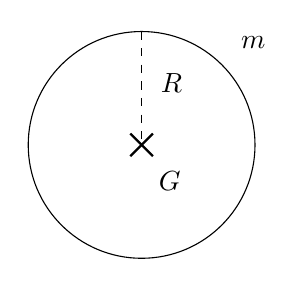
\begin{tikzpicture}[scale=1.2]
\draw (0,0) circle (1.2);
\draw[dashed] (0,1.2) -- (0,0);
\draw[thick] (-0.12,0.12) -- (0.12,-0.12);
\draw[thick] (-0.12,-0.12) -- (0.12,0.12);
\node[right] at (0.08,-0.38) {\(G\)};
\node[right] at (0.1,0.65) {\(R\)};
\node[right] at (0.95,1.08) {\(m\)};
\end{tikzpicture}
\end{center}

Sappiamo che \(I_G^{zz}=I_G=\frac{1}{2}mR^2\) e \(v_G=0\). Allora
\[
T=\frac{1}{2}\omega^2\cdot\frac{1}{2}mR^2=\frac{1}{4}mR^2\omega^2
\]
\end{example}


\begin{example}{}
Troviamo l'energia cinetica di un'asta con centro di massa fisso, lunghezza \(\ell\) e massa \(m\)

\begin{center}
\begin{tikzpicture}[scale=1.2,>=latex]
\draw[line width=0.8pt] (-1.2,-1.0) -- (1.2,1.0);

\fill (0,0) circle (2.2pt);
\draw[line width=0.8pt] (-0.12,0.12) -- (0.12,-0.12);
\draw[line width=0.8pt] (-0.12,-0.12) -- (0.12,0.12);

\node[left] at (-0.1,0.25) {\(G\)};
\node[right] at (1.02,1.18) {\(m\)};
\node[right] at (0.28,-0.52) {\(\ell\)};
\end{tikzpicture}
\end{center}

\[
I_G=\frac{m\ell^2}{12},\ v_G=0 \ \Rightarrow\ T=\frac{1}{2}\frac{m\ell^2}{12}\omega^2=\frac{m\ell^2\omega^2}{24}
\]
\end{example}
\begin{example}{}
Consideriamo ora un'asta di massa \(m\) e lunghezza \(\ell\) con un estremo fissato.

\begin{center}
\begin{tikzpicture}[scale=1.2,>=latex]
\coordinate (A) at (0,0);
\coordinate (B) at (2.6,-2.5);
\coordinate (C) at ($(A)!0.5!(B)$);

\draw[line width=0.8pt] (A) -- (B);
\draw[line width=0.8pt] (-0.08,0.18) -- (0.18,-0.08);
\draw[line width=0.8pt] (2.42,-2.32) -- (2.68,-2.58);

\draw[dashed] (A) -- (0,-2.7);

\draw[red,->] (A) -- (0.85,0);
\draw[red,->] (A) -- (0,0.95);

\node[red,right] at (0.7,0.02) {\(\hat{\imath}\)};
\node[red,left] at (0.05,0.88) {\(\hat{\jmath}\)};

\draw[thick] (A) circle (0.1);
\draw[thick] (-0.07,-0.07) -- (0.07,0.07);
\draw[thick] (-0.07,0.07) -- (0.07,-0.07);

\fill (C) circle (2pt);

\draw[->] (-0.05,-0.45) arc[start angle=-95,end angle=-50,radius=0.45];
\node[left] at (0.18,-0.92) {\(\theta\)};

\node[left] at (-0.15,0.02) {\(A\)};
\node[left] at ($(C)+(-0.08,0.15)$) {\(G\)};
\node[right] at (2.35,-2.75) {\(m\)};
\node[right] at (1.7,-1.05) {\(\ell\)};
\end{tikzpicture}
\end{center}

\[
x_G=\frac{\ell}{2}\sin\theta \qquad y_G=-\frac{\ell}{2}\cos\theta \qquad \Rightarrow \qquad \dot{x}_G=\dot{\theta}\frac{\ell}{2}\cos\theta \qquad \dot{y}_G=\dot{\theta}\frac{\ell}{2}\sin\theta
\]

Notiamo che
\[
v_G^2=\dot{x}_G^2+\dot{y}_G^2=\frac{\ell^2}{4}\dot{\theta}^2
\]
Allora
\[
T=\frac{m\ell^2\dot{\theta}^2}{8}+\frac{m\ell^2\dot{\theta}^2}{24}=\frac{m\ell^2\dot{\theta}^2}{6}=\frac{m\ell^2\omega^2}{6}
\]

Alternativamente potevamo lavorare con il teorema di Huygens e scrivere
\[
T=\frac{1}{2}I_A\omega^2=\frac{1}{2}\left(I_G+m\frac{\ell^2}{4}\right)\omega^2=\frac{1}{2}\left(\frac{m\ell^2}{12}+\frac{m\ell^2}{4}\right)\omega^2=\frac{m\ell^2}{6}\omega^2
\]
\end{example}
\begin{oss}{}
    L'uso dei momenti d'inerzia non rispetto ad un asse passante per il centro di massa per il calcolo dell'energia cinetica non l'abbiamo dimostrato in questo corso ma lo abbiamo fatto in Fisica 1 quindi lo diamo per buono!
\end{oss}

\begin{example}{}
Studiamo un disco di massa \(m\) e raggio \(r\) che rotola su una guida.

\begin{center}
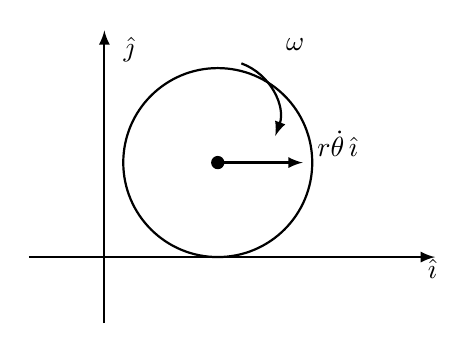
\begin{tikzpicture}[scale=1.2,>=latex]
\draw[->,line width=0.8pt] (-2,0) -- (2.3,0);
\draw[->,line width=0.8pt] (-1.2,-0.7) -- (-1.2,2.4);

\draw[line width=0.8pt] (0,1) circle (1);

\fill (0,1) circle (2pt);
\draw[->,line width=0.8pt] (0,1) -- (0.9,1);

\draw[->,line width=0.8pt] (0.25,2.05) arc[start angle=70,end angle=-20,radius=0.6];

\node[right] at (2.12,-0.12) {\(\hat{\imath}\)};
\node[right] at (-1.1,2.2) {\(\hat{\jmath}\)};
\node[right] at (0.95,1.2) {\(r\dot{\theta}\,\hat{\imath}\)};
\node[right] at (0.62,2.25) {\(\omega\)};
\end{tikzpicture}
\end{center}

Dal moto di puro rotolamento sappiamo che \(\underline{v_G}=r\dot{\theta}\,\hat{\imath}\)

\[
T=\frac{1}{2}m(r\dot{\theta})^2+\frac{1}{2}\left(\frac{1}{2}mr^2\right)\dot{\theta}^2=\frac{1}{2}mr^2\dot{\theta}^2+\frac{1}{4}mr^2\dot{\theta}^2=\frac{3}{4}mr^2\dot{\theta}^2
\]
\end{example}

\begin{example}{}
Studiamo il moto di un disco di massa \(M\) e raggio \(R\) che rotola su un piano orizzontale. Avvolto attorno al disco c'è un filo inestensibile teso e fatto passare attorno ad un piolo di altezza \(2R\). All'altra estremità del disco è appesa una massa \(m\). All'istante \(t=0\) lasciamo cadere la massa con velocità nulla e filo verticale dalla posizione del piolo.


\begin{center}
\begin{tikzpicture}[scale=1.15,>=latex]

% parametri
\def\R{1.4}

% piano
\draw[line width=1pt] (-3.2,0) -- (8.3,0);

% disco
\draw[line width=1pt] (0,\R) circle (\R);
\fill (0,\R) circle (2pt);

% punti A e C
\fill (0,2*\R) circle (2pt);
\fill (0,0) circle (2pt);
\node[above] at (0,2*\R) {\(A\)};
\node[below] at (0,0) {\(C\)};

% etichetta R,M
\node[left] at (-1.7,1.9) {\(R,M\)};

% peso disco
\draw[red,->,line width=1pt] (0,\R+0.2) -- (0,\R-0.7);
\node[red,right] at (0.1,\R-0.2) {\(\underline{Mg}\)};

% reazioni al contatto
\draw[green!60!black,->,line width=1pt] (0,0) -- (0.95,0);
\node[green!60!black,below] at (0.55,-0.05) {\(\underline{\psi_x}\)};

\draw[green!60!black,->,line width=1pt] (0,0) -- (0,0.95);
\node[green!60!black,left] at (-0.08,0.55) {\(\underline{\psi_y}\)};

% filo orizzontale e piolo
\draw[line width=1pt] (0,2*\R) -- (4.9,2*\R);
\draw[line width=1pt] (5.1,2*\R) circle (0.18);
\draw[line width=1pt] (5.1,2*\R-0.18) -- (5.1,1.05);

% massa appesa
\draw[line width=1pt] (4.95,1.05) rectangle (5.25,0.65);
\node[right] at (5.35,0.8) {\(m\)};

% tensioni
\draw[green!60!black,->,line width=1pt] (0.45,2*\R) -- (1.7,2*\R);
\node[green!60!black,above] at (0.95,2*\R+0.08) {\(\underline{\tau}\)};

\draw[green!60!black,->,line width=1pt] (5.1,0.65) -- (5.1,1.5);
\node[green!60!black,left] at (4.98,1.12) {\(\underline{\tau}\)};

% peso massa
\draw[red,->,line width=1pt] (5.1,0.65) -- (5.1,-0.25);
\node[red,right] at (5.2,0.15) {\(\underline{mg}\)};

% freccia di rotazione esterna al disco
\draw[->,line width=1pt] (1.25,2.45) arc[start angle=55,end angle=-35,radius=1.35];
\node[right] at (1.55,1.75) {\(\dot{\theta}\)};

% quota 2R
\draw[decorate,decoration={brace,amplitude=4pt}] (5.6,2*\R) -- (5.6,0);
\node[right] at (5.78,\R) {\(2R\)};

\end{tikzpicture}
\end{center}


Il sistema ha un grado di libertà: il puro rotolamento lascia un grado di libertà al disco e la massa è sottoposta ai vincoli
\[
\underline{x_m}=\underline{x_{\text{ext}}^{\text{asta}}}
\]

Vogliamo legare \(y_m\) con \(\theta\).

\[
\underline{v_A}=\underline{v_C}+\underline{\omega}\wedge(\underline{x_A}-\underline{x_C})=2R\dot{\theta}\,\hat{\imath}
\]

Per il vincolo di puro rotolamento tra disco e corda si ha che
\[
\underline{v_A}\cdot\hat{t}=\underline{v_A}^{\text{disco}}\cdot\hat{t}=\underline{v_A}^{\text{filo}}\cdot\hat{t}
\]

Inoltre dal momento che \(\hat{t}\parallel \underline{v_A}\) possiamo scrivere
\[
\dot{y}_m=-2R\dot{\theta}\Rightarrow y_m=-2R\theta
\]

Calcoliamo l'energia cinetica del sistema. Usando Huygens sappiamo che
\[
I_C=\frac{MR^2}{2}+MR^2=\frac{3}{2}MR^2 \Rightarrow T_s=\frac{3}{2}MR^2\frac{\dot{\theta}^2}{2}+\frac{m\dot{y}_m^2}{2}=\frac{3}{2}MR^2\frac{\dot{\theta}^2}{2}+\frac{m4R^2\dot{\theta}^2}{2}=R^2\dot{\theta}^2\left(\frac{3}{4}M+2m\right)
\]

Vogliamo infine trovare un'espressione analitica per \(\theta(t)\). Usiamo la prima legge cardinale su \(m\) e la seconda sul disco rispetto a \(C\) come polo.

\[
\left\{
\begin{aligned}
m\ddot{y}_m&=\tau-mg\\
\frac{d}{dt}(I_C\dot{\theta})&=2R\tau
\end{aligned}
\right.
\Rightarrow
\left\{
\begin{aligned}
-2mR\ddot{\theta}&=\tau-mg\\
\frac{3}{2}MR^2\ddot{\theta}&=2R\tau
\end{aligned}
\right.
\Rightarrow
\left\{
\begin{aligned}
-2mR\ddot{\theta}&=\frac{3}{4}MR\ddot{\theta}-mg\\
\tau&=\frac{3}{4}MR\ddot{\theta}
\end{aligned}
\right.
\]

\[
\Rightarrow \left(2mR+\frac{3}{4}MR\right)\ddot{\theta}=mg \Rightarrow \ddot{\theta}=\frac{mg}{2mR+\frac{3}{4}MR}
\]

\[
\theta(0)=0
\qquad
\dot{\theta}(0)=0
\]

\[
\Rightarrow \theta(t)=\frac{mg}{2mR+\frac{3}{4}MR}\frac{t^2}{2}
\]
\end{example}

\begin{example}{}
Studiamo una variazione dell'esercizio precedente: fissiamo il piolo ad altezza \(R\). Questa volta impongo le condizioni iniziali \(\theta(0)=1\) \(x_G(0)=R\) e fisso la rotazione positiva in senso antiorario.

\begin{center}
\begin{center}
\begin{tikzpicture}[scale=1.15,>=latex]

% parametri
\def\R{2}
\def\rp{0.18}

% punti principali
\coordinate (G) at (0,\R);
\coordinate (C) at (0,0);
\coordinate (A) at ({\R*cos(70)},{\R+\R*sin(70)});
\coordinate (P) at (5.84,\R);
\coordinate (B) at ($(P)+({\rp*cos(160)},{\rp*sin(160)})$);
\coordinate (O) at (4.65,0);

% piano
\draw[line width=0.9pt] (-4,0) -- (7.2,0);

% disco
\draw[line width=0.9pt] (G) circle (\R);

% punti
\fill (G) circle (2.3pt);
\fill (C) circle (2.3pt);
\fill (A) circle (2.3pt);

% etichette punti
\node[right] at ($(G)+(0.18,0.02)$) {\(G\)};
\node[below] at ($(C)+(0,-0.03)$) {\(C\)};
\node[above right] at ($(A)+(0.18,0.18)$) {\(A\)};

% raggio GA
\draw[line width=0.9pt] (G) -- (A);
\node[left] at ($(G)!0.55!(A)+(-0.08,0.08)$) {\(R\)};

% filo inclinato
\draw[line width=0.9pt] (A) -- (B);

% piolo
\draw[line width=0.9pt] (P) circle (\rp);

% filo verticale
\draw[line width=0.9pt] ($(P)+(0,-\rp)$) -- ($(P)+(0,-2.35)$);

% massa
\draw[line width=0.9pt] ($(P)+(-0.12,-2.65)$) rectangle ($(P)+(0.12,-2.35)$);
\node[right] at ($(P)+(0.32,-2.5)$) {\(m\)};

% linea tratteggiata orizzontale
\draw[dashed,line width=0.8pt] (G) -- (P);
\node[below] at ($(G)!0.55!(P)+(0,-0.18)$) {\(R\theta\)};

% angolo alpha
\draw[line width=0.8pt] ($(P)+(-0.55,0)$) arc[start angle=180,end angle=160,radius=0.55];
\node[above left] at ($(P)+(-0.7,0)$) {\(\alpha\)};

% squadra di ortogonalità in A
\draw[line width=0.8pt]
($(A)+(-0.08,-0.17)$) --
($(A)+(0.10,-0.24)$) --
($(A)+(0.17,-0.06)$);

% versore tangente
\draw[red,->,line width=1pt] (A) -- ++(-1.05,0.38);
\node[red,above] at ($(A)+(-0.62,0.48)$) {\(\hat{t}\)};

% freccia di theta
\draw[->,line width=1pt] (-2.35,3.95) arc[start angle=125,end angle=200,radius=1.15];
\node[left] at (-2.1,3.1) {\(\theta\)};

% velocità del centro
\draw[orange!85!black,->,line width=1pt] (G) -- ++(-1.45,0);
\node[orange!85!black,above] at ($(G)+(-0.78,0.14)$) {\(R\dot{\theta}\hat{\imath}\)};

% assi locali
\draw[green!60!black,->,line width=1pt] (O) -- ++(-0.95,0);
\draw[green!60!black,->,line width=1pt] (O) -- ++(0,0.95);
\node[green!60!black,below left] at ($(O)+(0.02,-0.02)$) {\(O\)};
\node[green!60!black,left] at ($(O)+(-0.58,-0.05)$) {\(\hat{\imath}\)};
\node[green!60!black,right] at ($(O)+(0.05,0.62)$) {\(\hat{\jmath}\)};

% quota R
\draw[decorate,decoration={brace,amplitude=4pt}] ($(P)+(0.45,0)$) -- ($(P)+(0.45,-\R)$);
\node[right] at ($(P)+(0.63,-1)$) {\(R\)};

\end{tikzpicture}
\end{center}
\end{center}

\[
R=R\theta\sin\alpha \Rightarrow \theta\sin\alpha=1 \Rightarrow \sin\alpha=\frac{1}{\theta} \Rightarrow \cos\alpha=\sqrt{1-\frac{1}{\theta^2}}=\sqrt{\frac{\theta^2-1}{\theta^2}} \qquad \text{con } |\theta|\geq 1
\]

Come prima \(\underline{v_A}=\underline{v_A}^{\text{disco}}=\underline{v_A}^{\text{filo}}\)

\[
\underline{v_G}=\omega\wedge(\underline{x_G}-\underline{x_C})=R\dot{\theta}\hat{\imath}
\]

\[
\underline{v_A}=\underline{v_G}+\omega\wedge(\underline{x_A}-\underline{x_G})=R\dot{\theta}\hat{\imath}+R\dot{\theta}\hat{t}
\]

Per sapere la velocità di \(m\) devo usare solo la componente lungo \(\hat{t}\)

\[
\Rightarrow \dot{y}_m=\underline{v_A}\cdot\hat{t}=R\dot{\theta}\hat{\imath}\cdot\hat{t}+R\dot{\theta}=R\dot{\theta}\left(1+\frac{\sqrt{\theta^2-1}}{\theta}\right)
\]

L'energia cinetica del sistema è

\[
T=\frac{3}{2}MR^2\frac{\dot{\theta}^2}{2}+\frac{m}{2}R^2\dot{\theta}^2\left(1+\frac{\sqrt{\theta^2-1}}{\theta}\right)^2
\]

Dalle equazioni cardinali si può ricavare \(\theta(t)\)

\[
\left\{
\begin{aligned}
M\ddot{x}_G&=\psi_x+\tau\cos\alpha\\
M\ddot{y}_G&=\psi_y-Mg+\tau\sin\alpha\\
m\ddot{y}_m&=mg+\tau\\
\frac{MR^2}{2}\ddot{\theta}&=-\psi_xR+\tau R
\end{aligned}
\right.
\]
\end{example}

\chapter{Principio dei lavori virtuali}
\begin{definition}{}[Lavoro di una forza]
Sia \(\underline{f}(\underline{x},\underline{v},t)\) una forza che agisce nel punto materiale di posizione \(\underline{x}(t)\), e velocità \(\underline{v}(t)\). Definiamo il lavoro della forza lungo la traiettoria \(\underline{x}(t)\) come
\[
L=\int_{\underline{x}} \underline{f}\cdot d\underline{x}
\]

\begin{center}
\begin{tikzpicture}[scale=1.1, >=Latex]

% assi
\draw[->, line width=0.8pt] (0,0) -- (-2.5,-2.7);
\draw[->, line width=0.8pt] (0,0) -- (3.2,0);
\draw[->, line width=0.8pt] (0,0) -- (0,2.3);

\node at (-2.65,-2.85) {\(x\)};
\node at (3.25,-0.45) {\(y\)};
\node at (0.35,2.35) {\(z\)};

% traiettoria
\draw[line width=0.8pt]
  (0.25,-1.2)
  .. controls (0.45,-0.2) and (0.8,0.4) ..
  (1.6,0.7)
  .. controls (2.4,1.0) and (2.9,1.7) ..
  (3.35,2.1);

% estremi e punto materiale
\fill (0.25,-1.2) circle (1.7pt);
\fill (3.35,2.1) circle (1.7pt);
\fill (1.7,0.62) circle (1.7pt);

\node at (1.05,0.95) {\(\underline{x}(t)\)};

% forza
\draw[->, line width=0.8pt] (1.7,0.62) -- (2.85,0.15);
\node at (2.75,0.7) {\(\underline{f}(\underline{x},\underline{v},t)\)};

\end{tikzpicture}
\end{center}
\end{definition}
Ricordiamo che ad ogni vincolo è associata una reazione vincolare che assicura il soddisfacimento del vincolo stesso.

\begin{definition}{}[Vincoli perfetti]
Un vincolo perfetto è un vincolo per il quale la reazione vincolare non compie lavoro, perché è \(\perp\) (localmente) alla traiettoria. Matematicamente un vincolo perfetto è tale che
\[
\underline{\Psi}\cdot \delta \underline{x}=0
\qquad
\forall\, \delta \underline{x}\ \text{compatibile con il vincolo}
\]
\end{definition}


Risulta necessario definire con chiarezza cosa siano i \(\delta \underline{x}\) e cosa voglia dire che questi siano ``compatibili con il vincolo''.
Lo facciamo nel caso in cui i vincoli siano regolari ma è possibile farlo anche in caso contrario.
Per fare ciò in modo matematicamente rigoroso abbiamo bisogno di strumenti di geometria differenziale avanzata e calcolo tensoriale che vanno al di là degli scopi del corso. Presenteremo quindi una trattazione meno rigorosa e più intuitiva basandoci su concetti di geometria differenziale di base rifacendoci soprattutto al caso noto delle superfici regolari.
\inizioapprof
I \(\delta \underline{x}\) vengono detti spostamenti virtuali. Supponiamo che un punto

materiale \((\underline{x}(t),m)\) sia soggetto al vincolo olonomo \(\overline{\Phi}(\underline{x},t)=0\).
Per ogni istante \(t\) definiamo la sottovarietà
\[
M_t=\{P\in\mathbb{R}^3:\overline{\Phi}(P,t)=0\}
\]

ovvero \(M_t=\overline{\Phi}^{-1}(0,t)\). Nel caso semplice in cui \(\underline{x}(t)\in\mathbb{R}^3\) questa può essere una superficie o una curva. In un caso più generale questa è una sotto-varietà dello spazio delle configurazioni \(Q\).
Se il vincolo è regolare, ovvero se \(d\overline{\Phi}(\underline{x},t)\) ha rango massimo \(\forall x\in\mathbb{R}^3\), allora \(M_t\) è una sottovarietà regolare. Risulta quindi definito in ogni punto \(\underline{x}\in M_t\) lo spazio tangente \(T_xM_t=\Ker(d\overline{\Phi}(\underline{x},t))\) a \(M_t\).
Per capire più facilmente questa condizione possiamo pensare al caso di superficie regolare ottenuta tramite controimmagine di un valore regolare: sia \(F:\mathbb{R}^3\to\mathbb{R}\) differenziabile e sia \(S=F^{-1}(0)\) con \(dF_p\) di rango massimo \(\forall p\in S\). In questo caso possiamo usare l'identificazione del funzionale \(dF_p:\mathbb{R}^3\to\mathbb{R}\) con il gradiente \(\nabla F_p\in\mathbb{R}^3\) data da \(dF_p(v)=\nabla F_p^Tv\ \ \forall v\in\mathbb{R}^3\).
Dire che \(dF_p\) ha rango massimo equivale a dire \(\nabla F_p\neq 0\) infatti \(\mathrm{rg}(dF_p)=\mathrm{rg}(L_{\nabla F_p})=0\) sse \(\nabla F_p=0\).
Allora lo spazio tangente non è altro che \(T_pS=\Ker(dF_p)=\{v\in\mathbb{R}: \nabla F_p^Tv=0\}\).\\
Gli spostamenti virtuali \(\delta \underline{x}\) sono in ogni istante fissato \(t\) gli elementi di \(T_{\underline{x}(t)}M_t\), ovvero sono le direzioni percorribili compatibili con la varietà \(M_t\) a \(t\) fissato.
È importante non confondere gli spostamenti virtuali \(\delta \underline{x}\) con gli spostamenti infinitesimi reali \(d\underline{x}=\underline{\dot{x}}(t)\,dt\).

I \(\delta \underline{x}\) sono tutti i possibili spostamenti percorribili in un tempo infinitesimo, sono una linearizzazione istantanea dei movimenti ammessi ma non è detto che questi vengano effettuati dalla traiettoria \(\underline{x}(t)\) (anzi al massimo uno di loro potrebbe essere effettuato ma non è detto che lo sia).

Dall'altra parte \(d\underline{x}=\underline{\dot{x}}(t)\,dt\) è effettivamente lo spostamento effettuato in un tempo infinitesimo \(dt\) dopo l'istante \(t\).\\
La differenza è netta tra i due nel caso di un vincolo dipendente dal tempo \(\overline{\Phi}(\underline{x},t)=0\). Immaginiamo due istanti di tempo \(t_1,t_2\) infinitesimamente vicini ai quali corrispondono le varietà \(M_{t_1},M_{t_2}\) con \(\underline{x}(t_1)\in M_{t_1}\), \(\underline{x}(t_2)\in M_{t_2}\).
Gli spostamenti virtuali stanno in \(T_{\underline{x}(t_1)}M_{t_1}\) e in \(T_{\underline{x}(t_2)}M_{t_2}\) che sono due spazi ben distinti. Lo spostamento reale infinitesimo invece è
\[
d\underline{x}=\underline{x}(t_2)-\underline{x}(t_1)\qquad (\text{abbiamo supposto } t_1-t_2\sim 0)
\]

che non sta in nessuno dei 2 tangenti.
Per capire meglio questo concetto pensiamo al caso del vincolo
\[
\overline{\Phi}(x,y,t)=(x-x_c(t))^2+(y-y_c(t))^2-R(t)^2=0
\]
Ad ogni istante \(t\) il punto è vincolato a muoversi su una circonferenza di raggio e centro variabile. Disegniamo spostamenti virtuali e spostamento reale per 2 istanti \(t_1,t_2\) molto vicini. \(C_1=(x_c(t_1),y_c(t_1))\), \(C_2=(x_c(t_2),y_c(t_2))\)
\begin{center}
\begin{tikzpicture}[scale=1,>=Latex]

% assi cartesiani
\draw[->, line width=1pt] (0.8,0.8) -- (0.8,6.2);
\draw[->, line width=1pt] (0.8,0.8) -- (9.4,0.8);
\node at (0.45,5.95) {\(y\)};
\node at (9.15,0.45) {\(x\)};

% circonferenze
\draw[line width=0.9pt] (3.0,2.2) circle (1.2);
\draw[line width=0.9pt] (7.4,4.2) circle (1.7);

% centri
\fill (3.0,2.2) circle (2pt);
\fill (7.4,4.2) circle (2pt);
\node at (2.75,1.75) {\(C_1\)};
\node at (7.15,3.75) {\(C_2\)};

% punti x(t1), x(t2)
\fill[purple] (3.8485,3.0485) circle (2.2pt);
\fill[purple] (6.3070,2.8978) circle (2.2pt);

\node[purple] at (4.55,3.35) {\(\underline{x}(t_1)\)};
\node[purple] at (6.95,2.45) {\(\underline{x}(t_2)\)};

% raggi
\draw[line width=0.9pt] (3.0,2.2) -- (3.8485,3.0485);
\draw[line width=0.9pt] (7.4,4.2) -- (6.3070,2.8978);

\node at (3.15,3.00) {\(R(t_1)\)};
\node at (6.45,3.95) {\(R(t_2)\)};

% tangente in x(t1)
\draw[line width=1pt, color=green!60!black] (3.32,3.58) -- (4.38,2.52);
\node[color=green!60!black] at (2.55,3.95) {\(T_{\underline{x}(t_1)}M\)};

% tangente in x(t2)
\draw[line width=1pt, color=red!80!black] (5.62,3.47) -- (6.99,2.33);
\node[color=red!80!black] at (8.25,2.55) {\(T_{\underline{x}(t_2)}M\)};

% vettore dx
\draw[->, line width=1pt, color=orange!90!black] (3.8485,3.0485) -- (6.3070,2.8978);
\node[color=orange!90!black] at (5.05,3.22) {\(\underline{dx}\)};

\end{tikzpicture}
\end{center}

Nel caso di vincolo costante si ha che \(M_t=M\ \forall t\) e che \(\underline{x}\in M\), \(d\underline{x}\in T_{\underline{x}}M\). Anche in questo caso però lo spostamento reale è un'entità distinta dagli spostamenti virtuali perché è l'unico che viene effettivamente effettuato.

\begin{oss}{}
Il concetto di spostamento virtuale si può generalizzare a un punto materiale soggetto a \(m\) vincoli olonomi differenziabili
\[
\overline{\Phi}_i(\underline{x},t)=0
\qquad
\forall i=1,\ldots,m
\]
in tal caso lo spazio dei \(\delta \underline{x}\) è \(T_{\underline{x}}M\) con
\[
M=\bigcap_{i=1}^{m}\Ker(d\overline{\Phi}_i)\Rightarrow \forall\,\delta \underline{x}\in T_{\underline{x}}M \quad d\overline{\Phi}_i\,\delta \underline{x}=0
\]

Allo stesso modo possiamo definire il concetto di spostamento virtuale per un sistema di \(n\) punti \(\underline{x}_1,\ldots,\underline{x}_n\) soggetto a \(m\) vincoli olonomi perfetti \(\overline{\Phi}_1(\underline{x}_1,\ldots,\underline{x}_n,t)\ldots \overline{\Phi}_m(\underline{x}_1,\ldots,\underline{x}_n,t)\).

Indichiamo una configurazione del sistema come
\[
\underline{x}=(\underline{x}_1,\ldots,\underline{x}_n)\in\mathbb{R}^{3n}.
\]
Imponendo i vincoli otteniamo
\[
M_t=\left\{\underline{x}\in\mathbb{R}^{3n}:\overline{\Phi}_1(\underline{x},t)=\ldots=\overline{\Phi}_m(\underline{x},t)=0\right\}
\]

Se i vincoli sono indipendenti e regolari su \(M_t\), ovvero il loro differenziale ha rango massimo su \(M_t\), quest'ultima è una sotto varietà regolare di \(\mathbb{R}^{3n}\) di dimensione \(r=3n-m\).

Uno spostamento virtuale \(\delta \underline{x}\) del sistema nella configurazione \(\underline{x}\in M_t\) è un vettore del tangente in \(\underline{x}\) a \(M_t\)
\[
\delta \underline{x}=(\delta \underline{x}_1,\ldots,\delta \underline{x}_n)\in T_{\underline{x}}M_t
\]

Importante notare che le \(\delta \underline{x}_i\) non sono arbitrarie proprio perché devono garantire \(\delta \underline{x}\in T_{\underline{x}}M_t\).

Si ha che
\[
T_{\underline{x}}M_t=\bigcap_{\nu=1}^{m}\Ker(d\overline{\Phi}_{\nu\,\underline{x}})=\left\{\delta \underline{x}:d\overline{\Phi}_{\nu\,\underline{x}}(\delta \underline{x})=0 \quad \forall \nu=1,\ldots,m\right\}
\]

Scrivendo in componenti
\[
T_{\underline{x}}M_t=\left\{\delta \underline{x}:\nabla \overline{\Phi}_\nu(\underline{x},t)^T\delta \underline{x}=0 \quad \forall \nu=1,\ldots,m\right\}=\mathrm{span}^{\perp}\left\{\nabla \overline{\Phi}_1(\underline{x},t),\ldots,\nabla \overline{\Phi}_m(\underline{x},t)\right\}
\]

ovvero è lo spazio ortogonale ai gradienti di tutti i vincoli in \(\underline{x}\).
\end{oss}

\begin{theorem}{}[Principio dei lavori virtuali, ipotesi semplificate, vincoli dipendenti solo da un punto]
Consideriamo un sistema meccanico formato dai punti \(\underline{x}_1,\ldots,\underline{x}_n\). Il punto \(\underline{x}_i\) è soggetto ai vincoli perfetti regolari
\[
\overline{\Phi}_{i,j}(\underline{x}_i)=0
\qquad
\forall j=1,\ldots,m_i.
\]
In ogni punto \(\underline{x}_i\) è esercitata una forza risultante
\[
\underline{f}_i=\underline{f}_i^{\mathrm{att.}}+\underline{f}_i^{\mathrm{reat.}}
\]
All'equilibrio vale la relazione
\[
\sum_{i=1}^{n}\underline{f}_i\cdot \delta \underline{x}_i=0
\qquad
\forall (\delta \underline{x}_1,\ldots,\delta \underline{x}_n)\in T_{\underline{x}_1}M_1\times\cdots\times T_{\underline{x}_n}M_n
\]
dove \(M_i\) è la varietà generata dai vincoli \(\{\overline{\Phi}_{i,j}(\underline{x}_i)\}_{j=1}^{m_i}\) e gli \(\delta \underline{x}_i\) sono gli spostamenti virtuali compatibili con i vincoli.
\end{theorem}

\begin{oss}{}
Similmente al concetto dei moltiplicatori di Lagrange stiamo dicendo che \(\forall i\) se \(\overline{\Phi}_{i,j}(\underline{x}_i)=0\) \(j=1,\ldots,m_i\): sono i vincoli perfetti imposti sul punto \(\underline{x}_i\) allora
\[
\underline{f}_i\in \mathrm{Span}\left\{\nabla \overline{\Phi}_{i,1}(\underline{x}_i),\ldots,\nabla \overline{\Phi}_{i,m_i}\right\}
\Longleftrightarrow
\underline{f}_i=\lambda_1\nabla \overline{\Phi}_{i,1}(\underline{x}_i)+\cdots+\lambda_{m_i}\nabla \overline{\Phi}_{i,m_i}
\]
\end{oss}
\begin{proof}
Sia \(M_i=\{\underline{x}_i\in\mathbb{R}^3:\overline{\Phi}_{i,1}(\underline{x}_i)=\ldots=\overline{\Phi}_{i,m_i}(\underline{x}_i)=0\}\) e sia \((\underline{x}_1,\ldots,\underline{x}_n)\in M_1\times\ldots\times M_n\).

Per ogni punto \(\underline{x}_i\) vale \(\underline{f}_i=\underline{f}_i^{\mathrm{att}}+\underline{f}_i^{\mathrm{reat}}\). Poiché i vincoli sono perfetti per ogni scelta di spostamenti virtuali ammessi vale
\[
\sum_{i=1}^{n}\underline{f}_i^{\mathrm{reat}}\cdot \delta \underline{x}_i=0
\qquad
(\delta \underline{x}_1,\ldots,\delta \underline{x}_n)\in T_{\underline{x}_1}M_1\times\ldots\times T_{\underline{x}_n}M_n
\]

Quindi la condizione sui lavori virtuali equivale a una sulle sole forze attive
\[
\sum_{i=1}^{n}\underline{f}_i\cdot \delta \underline{x}_i=0
\Longleftrightarrow
\sum_{i=1}^{n}\underline{f}_i^{\mathrm{att}}\cdot \delta \underline{x}_i=0
\]

Basta quindi dimostrare il teorema per la seconda condizione

\((\Rightarrow)\) Se siamo in una configurazione di equilibrio allora \(\forall i=1,\ldots,n\)
\[
\underline{f}_i^{\mathrm{att}}+\underline{f}_i^{\mathrm{reat}}=0
\]

Moltiplicando scalarmente per un qualsiasi \((\delta \underline{x}_1,\ldots,\delta \underline{x}_n)\) si ottiene
\[
\sum_{i=1}^{n}\underline{f}_i^{\mathrm{att}}\cdot \delta \underline{x}_i=
\sum_{i=1}^{n}\left(\underline{f}_i^{\mathrm{att}}+\underline{f}_i^{\mathrm{reat}}\right)\cdot \delta \underline{x}_i=0
\]

\((\Leftarrow)\) Supponiamo ora che
\[
\sum_{i=1}^{n}\underline{f}_i^{\mathrm{att}}\cdot \delta \underline{x}_i=0
\qquad
(\delta \underline{x}_1,\ldots,\delta \underline{x}_n)\in T_{\underline{x}_1}M_1\times\ldots\times T_{\underline{x}_n}M_n
\]

In particolare se scelgo un \(i\in\{1,\ldots,n\}\) deve essere vero per una configurazione del tipo \((0,\ldots,0,\delta \underline{x}_i,0,\ldots,0)\) con \(\delta \underline{x}_i\in T_{\underline{x}_i}M_i\) arbitrario. La condizione diventa
\[
\underline{f}_i^{\mathrm{att}}\cdot \delta \underline{x}_i=0
\qquad
\forall \delta \underline{x}_i\in T_{\underline{x}_i}M_i
\]

Quindi \(\underline{f}_i^{\mathrm{att}}\in (T_{\underline{x}_i}M_i)^{\perp}=\mathrm{span}\{\nabla \overline{\Phi}_{i,1}(\underline{x}_i),\ldots,\nabla \overline{\Phi}_{i,m_i}(\underline{x}_i)\}\Longleftrightarrow \exists \lambda_{i,1},\ldots,\lambda_{i,m_i} \in \mathbb{R}\) tali che
\[
\underline{f}_i^{\mathrm{att}}=\sum_{j=1}^{m_i}\lambda_{i,j}\nabla \overline{\Phi}_{i,j}(\underline{x}_i)
\]

Definiamo allora \(\underline{f}_i^{\mathrm{reat}}=-\sum_{j=1}^{m_i}\lambda_{i,j}\nabla \overline{\Phi}_{i,j}(\underline{x}_i)\). Ovviamente si ha \(\underline{f}_i^{\mathrm{att}}+\underline{f}_i^{\mathrm{reat}}=0\).

Abbiamo trovato una reazione vincolare compatibile con i vincoli che determina una configurazione di equilibrio valida per \(\underline{x}_i\). Dal momento che la \(i\) era arbitraria ho trovato una configurazione statica ammissibile per il sistema.
\end{proof}
\begin{theorem}{}[Principio dei lavori virtuali, vincoli regolari]
Consideriamo un sistema meccanico formato dai punti \(\underline{x}_1,\ldots,\underline{x}_n\) soggetto a \(m\) vincoli olonomi perfetti regolari
\[
\overline{\Phi}_1(\underline{x}_1,\ldots,\underline{x}_n,t)=\ldots=\overline{\Phi}_m(\underline{x}_1,\ldots,\underline{x}_n,t)=0.
\]
Supponiamo inoltre che in ogni punto agisca una risultante delle forze attive puramente posizionali \(\underline{f}_i^{\mathrm{att}}\). Allora siamo in una configurazione di equilibrio sse
\[
\sum_{i=1}^{n}\underline{f}_i^{\mathrm{att}}\cdot \delta \underline{x}_i=0
\qquad
\forall\, \delta \underline{x}=(\delta \underline{x}_1,\ldots,\delta \underline{x}_n)\in T_{\underline{x}}M_t
\]
dove \(M_t\) è la sottovarietà generata dai vincoli.
\end{theorem}
\begin{oss}{}
    Anche il principio dei lavori virtuali è valido nel caso in cui i vincoli siano solo olonomi perfetti ma non regolari. In questo caso però si perde la trattazione data dalla geometria differenziale e si deve procedere in altro modo.
\end{oss}
\begin{proof}
Indichiamo con \(\underline{R}=(\underline{R}_1,\ldots,\underline{R}_n)\) il sistema delle reazioni vincolari, allora dal momento che i vincoli sono perfetti vale
\[
\sum_{i=1}^{n}\underline{R}_i\cdot \delta \underline{x}_i=0
\qquad
\forall\, \delta \underline{x}=(\delta \underline{x}_1,\ldots,\delta \underline{x}_n)\in T_{\underline{x}}M_t
\]
ovvero \(\underline{R}\in T_{\underline{x}}M_t^\perp\).

\((\Rightarrow)\) Supponiamo \(\underline{x}\) di equilibrio, per definizione esistono le reazioni vincolari \(\underline{R}_1,\ldots,\underline{R}_n\) tali che
\[
\underline{f}_i^{\mathrm{att}}+\underline{R}_i=0
\qquad
\forall i=1,\ldots,n
\]
Sia \(\delta \underline{x}\) uno spostamento virtuale arbitrario. Allora
\[
0=\sum_{i=1}^{n}\left(\underline{f}_i^{\mathrm{att}}+\underline{R}_i\right)\cdot \delta \underline{x}_i
=\sum_{i=1}^{n}\underline{f}_i^{\mathrm{att}}\cdot \delta \underline{x}_i
\]

\((\Leftarrow)\) Supponiamo ora che
\[
\sum_{i=1}^{n}\underline{f}_i^{\mathrm{att}}\cdot \delta \underline{x}_i=0
\qquad
\forall\, \delta \underline{x}=(\delta \underline{x}_1,\ldots,\delta \underline{x}_n)\in T_{\underline{x}}M_t
\]
Introduciamo il vettore globale delle forze attive
\[
\underline{A}=(\underline{f}_1^{\mathrm{att}},\ldots,\underline{f}_n^{\mathrm{att}})\in\mathbb{R}^{3n},
\]
la condizione si riscrive come
\[
\underline{A}\cdot \delta \underline{x}=0
\qquad
\forall\, \delta \underline{x}\in T_{\underline{x}}M_t
\Longleftrightarrow
\underline{A}\in T_{\underline{x}}M_t^\perp
\]
Siccome i vincoli sono regolari
\[
T_{\underline{x}}M_t^\perp=\mathrm{Span}\left\{\nabla \overline{\Phi}_{1\underline{x}},\ldots,\nabla \overline{\Phi}_{m\underline{x}}\right\},
\]
perciò esistono $\lambda_1, \dots, \lambda_m \in \mathbb{R}$ tali che
\[
\underline{A}=\sum_{j=1}^{m}\lambda_j\,\nabla \overline{\Phi}_{j\underline{x}}
\]
Definiamo ora \(\underline{R}=-\underline{A}\). Per definizione \(\underline{R}\in T_{\underline{x}}M_t^\perp\) ed è quindi una reazione vincolare ammissibile. Se riscriviamo la condizione \(\underline{A}+\underline{R}=0\) per blocchi otteniamo
\[
(\underline{f}_1^{\mathrm{att}},\ldots,\underline{f}_n^{\mathrm{att}})+(\underline{R}_1,\ldots,\underline{R}_n)=0
\]
che scritta componente per componente è
\[
\underline{f}_i^{\mathrm{att}}+\underline{R}_i=0
\qquad
\forall i=1,\ldots,n
\]
ovvero la condizione di equilibrio.

Abbiamo quindi dimostrato che il principio dei lavori virtuali è condizione necessaria e sufficiente per l'equilibrio.
\end{proof}
\fineapprof
Consideriamo un sistema meccanico con \(n\) punti, \(3n\) gradi di libertà, \(m\) vincoli olonomi perfetti regolari.

Poiché i vincoli sono anche olonomi possiamo determinare \(q_1,\ldots,q_{3n-m}\) coordinate libere.
Le posizioni \(\underline{x}_i(t)\) sono univocamente determinate dalle coordinate libere
\[
\underline{x}_i(q_1(t),\ldots,q_{3n-m}(t))
\]

Possiamo considerare gli spostamenti virtuali nello spazio delle variabili libere.
Localmente il differenziale di \(\underline{x}_i(q_1,\ldots,q_{3n-m})\) manda un \(\delta \underline{q}=(\delta q_1,\ldots,\delta q_{3n-m})\) in un \(\delta \underline{x}_i\), ovvero
\[
\delta \underline{x}_i=d\underline{x}_{i,\underline{q}}(\delta \underline{q})
\]

In coordinate
\[
\delta \underline{x}_i=\sum_{j=1}^{3n-m}\frac{\partial \underline{x}_i}{\partial q_j}(\underline{q})\,\delta q_j
\]

\begin{example}{}
Consideriamo un punto che si muove su una circonferenza. \(i=1\) \(q=\theta\).
\[
\underline{x}_1=(R\cos\theta,R\sin\theta)
\]

\[
\delta \underline{x}=\frac{\partial \underline{x}}{\partial q}\cdot \delta q
=\frac{\partial \underline{x}}{\partial \theta}\cdot \delta \theta
=\frac{\partial}{\partial \theta}
\begin{pmatrix}
R\cos\theta\\
R\sin\theta
\end{pmatrix}
\delta \theta
=
\begin{pmatrix}
-R\sin\theta\,\delta \theta\\
R\cos\theta\,\delta \theta
\end{pmatrix}
\]
\end{example}

Se metto questa rappresentazione dello spostamento virtuale in funzione delle coordinate libere nel principio dei lavori virtuali ottengo
\[
\sum_{i=1}^{n}\underline{f}_i\cdot \delta \underline{x}_i
=
\sum_{i=1}^{n}\underline{f}_i^{\mathrm{att}}\cdot \delta \underline{x}_i
=
\sum_{i=1}^{n}\underline{f}_i^{\mathrm{att}}\cdot \sum_{j=1}^{3n-m}\frac{\partial \underline{x}_i}{\partial q_j}\,\delta q_j
=
\sum_{j=1}^{3n-m}\left(\sum_{i=1}^{n}\underline{f}_i\cdot \frac{\partial \underline{x}_i}{\partial q_j}\right)\delta q_j
\]

Chiamiamo
\[
\sum_{i=1}^{n}\underline{f}_i\cdot \frac{\partial \underline{x}_i}{\partial q_j}=Q_j
\qquad \Rightarrow \qquad
\sum_{i=1}^{n}\underline{f}_i\cdot \delta \underline{x}_i
=
\sum_{j=1}^{3n-m}Q_j\,\delta q_j
\]

Possiamo dare un'altra dimostrazione del principio dei lavori virtuali basato sulla parametrizzazione locale della varietà attraverso le coordinate libere.
\begin{proof}
Alternativamente si può procedere in coordinate libere. Si ha
\[
\sum_{i=1}^{n} \underline{f}_i^{\mathrm{att}}\cdot \delta \underline{x}_i
=
\sum_{i=1}^{n} \underline{f}_i^{\mathrm{att}}\cdot
\sum_{j=1}^{3n-m}
\frac{\partial \underline{x}_i}{\partial q_j}\,\delta q_j
=
\sum_{j=1}^{3n-m}
\left(
\underbrace{
\sum_{i=1}^{n}
\underline{f}_i^{\mathrm{att}}\cdot
\frac{\partial \underline{x}_i}{\partial q_j}
}_{Q_j}
\right)
\delta q_j.
\]

Dal momento che
\[
\underline{Q}\cdot
\begin{pmatrix}
\delta q_1\\
\vdots\\
\delta q_{3n-m}
\end{pmatrix}
=0
\qquad
\forall\,(\delta q_1,\dots,\delta q_{3n-m}),
\]
segue che
\[
\underline{Q}=\underline{0}
\qquad \Longrightarrow \qquad
Q_j=0
\quad
\forall j=1,\dots,3n-m.
\]

Allora la risultante delle forze attive è perpendicolare allo spazio delle direzioni ammesse dai vincoli e arriviamo alla stessa conclusione di prima.
\end{proof}

\begin{example}{}
  Studiamo la statica del seguente sistema.
  \begin{center}
    \begin{tikzpicture}[
    x=1cm,
    y=1cm,
    >=Latex,
    line cap=round,
    line join=round,
    every node/.style={font=\small}
]

% Parametri
\def\R{1.55}

% Coordinate
\coordinate (O) at (0,0);
\coordinate (A) at (0,3.45);
\coordinate (G) at (7.20,\R);
\coordinate (C) at (7.20,0);
\coordinate (Top) at ($(G)+(0,\R)$);
\coordinate (B) at ($(A)!0.42!(G)$);

% Assi
\draw[black, line width=1.4pt, ->] (0,0) -- (10.2,0) node[below right] {$x$};
\draw[black, line width=1.4pt, ->] (0,0) -- (0,4.2) node[above left] {$y$};

% Parete verticale
\draw[black, line width=2pt] (0,0) -- (0,4.05);

% Origine
\node[below left] at (O) {$O$};

% Riferimento centrato in O
\draw[orange!85!black, line width=1.4pt, ->] (O) -- ++(0.95,0);
\draw[orange!85!black, line width=1.4pt, ->] (O) -- ++(0,0.95);
\node[orange!85!black, below] at ($(O)+(0.48,0)$) {$\underline{\imath}$};
\node[orange!85!black, left] at ($(O)+(0,0.48)$) {$\underline{\jmath}$};

\draw[orange!85!black, line width=1.2pt] (-0.45,0.18) circle (0.18);
\fill[orange!85!black] (-0.45,0.18) circle (0.03);
\node[orange!85!black, left] at (-0.62,0.62) {$\underline{k}$};

% Sbarrette verticali attaccate all'asse y
\draw[black, line width=1.6pt] (0,3.14) -- (0,3.56);
\draw[black, line width=1.6pt] (0.12,3.14) -- (0.12,3.56);

% Punto A
\node[left] at (A) {$A$};

% Asta
\draw[black, line width=1.8pt] (A) -- (G);

% Punto B
\fill[red] (B) circle (2.8pt);
\node[above] at (B) {$B$};

% Etichetta asta
\node[above right] at ($(B)!0.52!(G)$) {$l,m$};

% Angolo theta
\draw[black, line width=1.1pt]
($(A)+(0,-0.78)$) arc[start angle=-90,end angle=-14.5,radius=0.78];
\node at ($(A)+(0.72,-0.87)$) {$\theta$};

% Freccia verde in A
\draw[green!55!black, line width=1.4pt, ->] ($(A)$) -- ++(1.80,0);
\node[green!55!black, above] at ($(A)+(1.25,0.20)$) {$\underline{\psi}$};

% Molla attaccata all'asse y
\draw[black, line width=1.4pt, smooth, samples=240, domain=0:7.02]
plot (\x,{1.55 + 0.10*sin(900*\x)});

% Ruota
\draw[black, line width=1.8pt] (G) circle (\R);

% Punto C
\node[below] at (C) {$C$};

% Centro G
\filldraw[white, draw=black, line width=1.2pt] (G) circle (0.09);
\node[above left] at ($(G)+(-0.10,0.08)$) {$G$};

% Etichetta M,R
\node[above right] at ($(Top)+(0.95,-0.05)$) {$M,R$};

% Raggi tratteggiati
\draw[black, dashed, line width=1.1pt] (Top) -- (G);
\draw[black, dashed, line width=1.1pt] (G) -- ++(0.95,1.00);

% Angolo phi
\draw[black, line width=1.0pt, ->]
($(G)+(0,0.58)$) arc[start angle=90,end angle=46,radius=0.58];
\node at ($(G)+(0.47,0.92)$) {$\varphi$};

% Forza mg in B
\draw[red!85!black, line width=1.5pt, ->] (B) -- ++(0,-1.15);
\node[red!85!black, left] at ($(B)+(0.10,-0.70)$) {$m\underline{g}$};

% Forza Mg in G
\draw[red!85!black, line width=1.5pt, ->] (G) -- ++(0,-1.05);
\node[red!85!black, right] at ($(G)+(0.52,-0.62)$) {$M\underline{g}$};

% Forza elastica
\draw[red!85!black, line width=1.5pt, ->] (G) -- ++(-1.25,0);
\node[red!85!black, below] at ($(G)+(-0.82,-0.12)$) {$-k\,\underline{x}_G$};

% Assi verdi vicino a C
\draw[green!55!black, line width=1.4pt, ->] ($(C)+(0.18,0)$) -- ++(1.90,0);
\draw[green!55!black, line width=1.4pt, ->] ($(C)+(0.18,0)$) -- ++(0,0.95);
\node[green!55!black, right] at ($(C)+(2.10,0)$) {$\underline{\xi}_x$};
\node[green!55!black, right] at ($(C)+(0.22,0.58)$) {$\underline{\xi}_y$};

\end{tikzpicture}
  \end{center}
Imposto un riferimento fisso
\[
\{O,\hat{\imath},\hat{\jmath},\hat{k}\}.
\]
Il sistema è soggetto ai vincoli
\[
\left\{
\begin{array}{l}
x_G^{\mathrm{disco}}=x_G^{\mathrm{asta}},\\[2mm]
y_G^{\mathrm{disco}}=y_G^{\mathrm{asta}}.
\end{array}
\right.
\]

Come coordinata libera posso scegliere $\theta$, $\psi$ o $x_G$.
Supponendo che per $\psi=0$ il corpo sia in $x_G=0$, si ha
\[
l\sin\theta = R\psi = x_G.
\]

Scrivo le equazioni della statica per i due corpi:
\[
\left\{
\begin{array}{l}
\underline{\psi}
+
m\underline{g}
+
M\underline{g}
-
k\underline{x}_G
+
\underline{\xi}_x
+
\underline{\xi}_y
=
\underline{0},
\\[2mm]
\left(\underline{x}_C-\underline{x}_G\right)\wedge \underline{\xi}_x
=
\underline{0},
\\[2mm]
\left(\underline{x}_B-\underline{x}_G\right)\wedge m\underline{g}
+
\left(\underline{x}_A-\underline{x}_G\right)\wedge \underline{\psi}
=
\underline{0}.
\end{array}
\right.
\]

Dove nella prima ho accorpato la prima legge cardinale per i due corpi
attraverso il principio di azione e reazione.

\[
\left\{
\begin{array}{l}
\psi-kx_G+\xi_x=0,
\\[1mm]
-mg-Mg+\xi_y=0,
\\[1mm]
-R\xi_x=0,
\\[1mm]
mg\dfrac{l}{2}\sin\theta-l\psi\cos\theta=0.
\end{array}
\right.
\]

Quindi
\[
\left\{
\begin{array}{l}
\psi=kl\sin\theta,
\\[1mm]
\xi_y=mg+Mg,
\\[1mm]
mg\dfrac{l}{2}\sin\theta
-
l\cos\theta\,kl\sin\theta
=0.
\end{array}
\right.
\]

Da cui
\[
mg\sin\theta-2kl\sin\theta\cos\theta=0.
\]

Se
\[
\sin\theta=0,
\]
allora
\[
\theta_1=0,
\qquad
\theta_2=\pi.
\]

Se invece
\[
\sin\theta\neq 0,
\]
allora
\[
mg-2kl\cos\theta=0
\]
e quindi
\[
\cos\theta_{3,4}
=
\frac{mg}{2kl},
\qquad
\frac{mg}{2kl}\leq 1.
\]

Dal momento che
\[
\cos\theta_{3,4}>0,
\]
le configurazioni di equilibrio sono le seguenti.
\begin{center}
  \begin{tikzpicture}[scale=1, line cap=round, line join=round, >=Latex]

%======================
% Disegno 1
%======================
\begin{scope}[shift={(0,0)}]
    \node at (0,3.35) {$\theta_1=0$};

    % piano
    \draw[line width=0.9pt] (-1.7,0) -- (1.7,0);

    % disco
    \draw[line width=1pt] (0,1) circle (1);

    % asta verticale
    \draw[line width=1pt] (0,1) -- (0,2.85);

    % punto A e guida
    \fill (0,2.15) circle (1.2pt);
    \node[right] at (0,2.15) {$A$};
    \draw[line width=0.8pt] (-0.13,1.90) -- (-0.13,2.40);
    \draw[line width=0.8pt] ( 0.13,1.90) -- ( 0.13,2.40);
\end{scope}

%======================
% Disegno 2
%======================
\begin{scope}[shift={(5.6,0)}]
    \node at (0,3.35) {$\theta_2=\pi$};

    % piano
    \draw[line width=0.9pt] (-1.7,0) -- (1.7,0);

    % disco
    \draw[line width=1pt] (0,1) circle (1);

    % asta verticale verso il basso
    \draw[line width=1pt] (0,1) -- (0,-1.05);

    % punto A e guida
    \fill (0,-0.38) circle (1.2pt);
    \node[right] at (0,-0.38) {$A$};
    \draw[line width=0.8pt] (-0.13,-0.63) -- (-0.13,-0.13);
    \draw[line width=0.8pt] ( 0.13,-0.63) -- ( 0.13,-0.13);
\end{scope}

%======================
% Disegno 3
%======================
\begin{scope}[shift={(12.4,0)}]
    \node at (0,3.35) {$\theta_3,\theta_4$};

    % piano con freccia
    \draw[line width=0.9pt, ->] (-3.3,0) -- (4.2,0);

    % asse verticale centrale
    \draw[line width=1pt] (0,-1.4) -- (0,2.95);

    % dischi
    \draw[line width=1pt] (-1.7,1) circle (1);
    \draw[line width=1pt] ( 1.7,1) circle (1);

    % centri dei dischi
    \coordinate (GL) at (-1.7,1);
    \coordinate (GR) at ( 1.7,1);
    \coordinate (A)  at (0,2.18);

    % punto A e guida
    \fill (A) circle (1.2pt);
    \node[right] at (A) {$A$};
    \draw[line width=0.8pt] (-0.13,1.92) -- (-0.13,2.42);
    \draw[line width=0.8pt] ( 0.13,1.92) -- ( 0.13,2.42);

    % aste inclinate che partono dai centri delle circonferenze
    \draw[line width=1pt] (GL) -- (A);
    \draw[line width=1pt] (GR) -- (A);

    % molla orizzontale tra i due centri
    \draw[line width=1pt] (-1.7,1) -- (-1.25,1);

    \draw[line width=1pt, smooth, samples=100, domain=-1.25:-0.15]
        plot (\x,{1 + 0.07*sin((\x+1.25)/1.10*1080)});

    \fill (0,1) circle (1.2pt);

    \draw[line width=1pt, smooth, samples=100, domain=0.15:1.25]
        plot (\x,{1 + 0.07*sin((\x-0.15)/1.10*1080)});

    \draw[line width=1pt] (1.25,1) -- (1.7,1);
\end{scope}

\end{tikzpicture}
\end{center}

Troviamo le stesse posizioni con il principio dei lavori virtuali:
\[
-mg\hat{\jmath}\cdot \delta \underline{x}_B
-Mg\hat{\jmath}\cdot \delta \underline{x}_G
-kl\sin\theta\,\hat{\imath}\cdot \delta \underline{x}_G
=0
\qquad
\forall\,(\delta \underline{x}_B,\delta \underline{x}_G)
\text{ ammessi}.
\]

Passo alla coordinata libera:
\[
\underline{x}_B
=
\frac{l}{2}\sin\theta\,\hat{\imath}
+
\left(
R+\frac{l}{2}\cos\theta
\right)\hat{\jmath},
\qquad
\underline{x}_G
=
l\sin\theta\,\hat{\imath}
+
R\hat{\jmath}.
\]

Quindi
\[
\delta \underline{x}_B
=
\frac{l}{2}\cos\theta\,\delta\theta\,\hat{\imath}
-
\frac{l}{2}\sin\theta\,\delta\theta\,\hat{\jmath},
\qquad
\delta \underline{x}_G
=
l\cos\theta\,\delta\theta\,\hat{\imath}.
\]

Allora
\[
-mg\hat{\jmath}\cdot
\left(
-\frac{l}{2}\sin\theta\,\delta\theta\,\hat{\jmath}
\right)
-
Mg\hat{\jmath}\cdot
\left(
l\cos\theta\,\delta\theta\,\hat{\imath}
\right)
-
kl\sin\theta\,\hat{\imath}\cdot
\left(
l\cos\theta\,\delta\theta\,\hat{\imath}
\right)
=0.
\]

Da cui
\[
mg\frac{l}{2}\sin\theta\,\delta\theta
-
kl\sin\theta\,l\cos\theta\,\delta\theta
=0
\qquad
\forall\,\delta\theta.
\]

Pertanto
\[
mg\frac{l}{2}\sin\theta
-
kl\sin\theta\,l\cos\theta
=0.
\]

Equivalentemente,
\[
mg\sin\theta
-
2kl\sin\theta\cos\theta
=0.
\]

Quindi
\[
\theta_1=0,
\qquad
\theta_2=\pi,
\qquad
\cos\theta_{3,4}
=
\frac{mg}{2kl},
\qquad
\frac{mg}{2kl}\leq 1.
\]
\end{example}

\vspace{60pt}
\begin{example}{}
  Studiamo la statica del seguente sistema.
  \begin{center}
    \begin{tikzpicture}[
    x=1cm,
    y=1cm,
    >=Latex,
    line cap=round,
    line join=round,
    every node/.style={font=\small}
]

% Coordinate principali
\coordinate (O) at (0,0);
\coordinate (A) at (2.70,0);
\coordinate (C) at (6.10,0);
\coordinate (B) at (6.10,-2.35);
\coordinate (G) at ($(A)!0.47!(B)$);

% Riferimento a sinistra
\draw[blue!70!black, line width=1.4pt, ->] (O) -- ++(0,1.10);
\draw[blue!70!black, line width=1.4pt, ->] (O) -- ++(0.85,0);
\node[blue!70!black, left]  at ($(O)+(0,0.60)$) {$\underline{\jmath}$};
\node[blue!70!black, below] at ($(O)+(0.42,0)$) {$\underline{\imath}$};

\draw[blue!70!black, line width=1.2pt] ($(O)+(-0.55,-0.45)$) circle (0.20);
\fill[blue!70!black] ($(O)+(-0.55,-0.45)$) circle (0.035);
\node[blue!70!black, left]  at ($(O)$) {$O$};
\node[blue!70!black, below] at ($(O)+(-0.55,-0.72)$) {$\underline{k}$};

% Molla sinistra attaccata al riferimento
\draw[yellow!80!orange!90!black, line width=1.4pt] (O) -- (0.22,0);
\draw[yellow!80!orange!90!black, line width=1.4pt, smooth, samples=140, domain=0.22:2.48]
plot (\x,{0.16*sin(deg((\x-0.22)*15.5))});
\draw[yellow!80!orange!90!black, line width=1.4pt] (2.48,0) -- (A);
\node at (1.00,0.55) {$K$};

% Tratto orizzontale superiore
\draw[black, line width=1.2pt] (0,0) -- (7.05,0);

% Asta inclinata
\draw[black, line width=1.2pt] (A) -- (B);

% Molla destra verticale
\draw[yellow!80!orange!90!black, line width=1.4pt] (C) -- ++(0,-0.22);
\draw[yellow!80!orange!90!black, line width=1.4pt, smooth, samples=140, domain=-0.22:-2.13]
plot ({6.10 + 0.10*sin(deg((\x+0.22)*16.5))}, \x);
\draw[yellow!80!orange!90!black, line width=1.4pt] (6.10,-2.13) -- (B);
\node[right] at ($(C)+(0.45,-1.15)$) {$K$};

% Punti e nomi
\node[below left]  at (A) {$A$};
\node[above]       at (C) {$C$};
\node[below right] at (B) {$B$};
\node[below]       at ($(B)+(-0.45,-0.10)$) {$m,l$};

\fill[black] (G) circle (1.6pt);
\node[right] at ($(G)+(0.05,0.05)$) {$G$};

% Angolo theta
\draw[black, line width=1.0pt]
($(A)+(0.65,0)$) arc[start angle=0,end angle=-38,radius=0.65];
\node at ($(A)+(0.82,-0.40)$) {$\theta$};

% Freccia rossa F
\draw[red!80!black, line width=1.5pt, ->] ($(A)+(0.05,0)$) -- ++(1.05,0);
\node[red!80!black, above] at ($(A)+(0.55,0.38)$) {$\underline{F}$};

% Freccia verde psi in A
\draw[green!55!black, line width=1.4pt, ->] ($(A)+(0,-0.05)$) -- ++(0,-0.60);
\node[green!55!black, right] at ($(A)+(0.10,-0.47)$) {$\underline{\psi}$};

% Forza elastica sinistra
\draw[red!80!black, line width=1.5pt, ->] ($(A)+(-0.25,-0.55)$) -- ++(-1.10,0);
\node[red!80!black, below] at ($(A)+(-0.80,-0.55)$) {$-k\,\underline{x}_A$};

% Peso in G
\draw[red!80!black, line width=1.5pt, ->] (G) -- ++(0,-1.00);
\node[red!80!black, left] at ($(G)+(-0.10,-0.68)$) {$m\underline{g}$};

% Forza elastica destra
\draw[red!80!black, line width=1.5pt, ->] ($(C)+(1.20,-2.00)$) -- ++(0,1.10);
\node[red!80!black, right] at ($(C)+(1.40,-1.45)$)
{$K\big(\underline{x}_C-\underline{x}_B\big)$};

\end{tikzpicture}
  \end{center}
  Imposto un riferimento fisso
\[
\{O,\hat{\imath},\hat{\jmath},\hat{k}\}.
\]
L'asta di lunghezza \(l\) e massa \(m\) è sottoposta al vincolo
\[
y_A^{\mathrm{asta}}=0
\]
ed ha quindi \(2\) gradi di libertà. Scelgo come coordinate libere
\[
x_A,\theta.
\]
Studiamo le sue equazioni della statica:
\[
\left\{
\begin{array}{l}
\underline{F}
-k\underline{x}_A
+\underline{\psi}
+m\underline{g}
+k\left(\underline{x}_C-\underline{x}_B\right)
=
\underline{0},
\\[2mm]
\left(\underline{x}_G-\underline{x}_A\right)\wedge m\underline{g}
+
\left(\underline{x}_B-\underline{x}_A\right)\wedge
k\left(\underline{x}_C-\underline{x}_B\right)
=
\underline{0}
\qquad
\text{polo } A.
\end{array}
\right.
\]

Quindi
\[
\left\{
\begin{array}{l}
F\hat{\imath}
-kx_A\hat{\imath}
-\psi\hat{\jmath}
-mg\hat{\jmath}
+kl\sin\theta\,\hat{\jmath}
=
\underline{0},
\\[2mm]
\dfrac{l}{2}
\left(
\cos\theta\,\hat{\imath}
-
\sin\theta\,\hat{\jmath}
\right)
\wedge
\left(
-mg\hat{\jmath}
\right)
+
l
\left(
\cos\theta\,\hat{\imath}
-
\sin\theta\,\hat{\jmath}
\right)
\wedge
kl\sin\theta\,\hat{\jmath}
=
\underline{0}.
\end{array}
\right.
\]

Passando alle componenti:
\[
\left\{
\begin{array}{l}
F-kx_A=0,
\\[1mm]
-\psi-mg+kl\sin\theta=0,
\\[1mm]
-\dfrac{l}{2}\cos\theta\,mg
+
l\cos\theta\,kl\sin\theta
=0.
\end{array}
\right.
\]

Dalla prima equazione:
\[
x_A=\frac{F}{k}.
\]

Dalla terza equazione:
\[
-\frac{l}{2}\cos\theta\,mg
+
kl^2\sin\theta\cos\theta
=0,
\]
cioè
\[
2kl\sin\theta\cos\theta
-
mg\cos\theta
=0.
\]

Se
\[
\cos\theta=0,
\]
allora
\[
\theta_1=\frac{\pi}{2},
\qquad
\theta_2=\frac{3}{2}\pi.
\]

Se invece
\[
\cos\theta\neq 0,
\]
allora
\[
2kl\sin\theta=mg,
\]
da cui
\[
\sin\theta=\frac{mg}{2kl}.
\]

Quindi
\[
\sin\theta_{3,4}
=
\frac{mg}{2kl},
\qquad
\frac{mg}{2kl}\leq 1.
\]

Facciamolo con il principio dei lavori virtuali:
\[
-k\underline{x}_A\cdot \delta\underline{x}_A
+
\underline{F}\cdot \delta\underline{x}_A
+
m\underline{g}\cdot \delta\underline{x}_G
+
k\left(\underline{x}_C-\underline{x}_B\right)\cdot
\delta\underline{x}_B
=
0.
\]

Scrivo gli spostamenti virtuali in coordinate libere:
\[
\underline{x}_A
=
x_A\hat{\imath}
\qquad \Longrightarrow \qquad
\delta\underline{x}_A
=
\delta x_A\hat{\imath}.
\]

\[
\underline{x}_G
=
\underline{x}_G-\underline{x}_A+\underline{x}_A
=
\frac{l}{2}
\left(
\cos\theta\,\hat{\imath}
-
\sin\theta\,\hat{\jmath}
\right)
+
x_A\hat{\imath},
\]
quindi
\[
\delta\underline{x}_G
=
\delta x_A\hat{\imath}
-
\frac{l}{2}\sin\theta\,\delta\theta\,\hat{\imath}
-
\frac{l}{2}\cos\theta\,\delta\theta\,\hat{\jmath}.
\]

Analogamente,
\[
\underline{x}_B
=
\underline{x}_B-\underline{x}_A+\underline{x}_A
=
l
\left(
\cos\theta\,\hat{\imath}
-
\sin\theta\,\hat{\jmath}
\right)
+
x_A\hat{\imath},
\]
quindi
\[
\delta\underline{x}_B
=
\delta x_A\hat{\imath}
-
l\sin\theta\,\delta\theta\,\hat{\imath}
-
l\cos\theta\,\delta\theta\,\hat{\jmath}.
\]

Sostituendo nel principio dei lavori virtuali:
\[
-Kx_A\hat{\imath}\cdot \delta x_A\hat{\imath}
+
F\hat{\imath}\cdot \delta x_A\hat{\imath}
-
mg\hat{\jmath}\cdot
\left(
\delta x_A\hat{\imath}
-
\frac{l}{2}\sin\theta\,\delta\theta\,\hat{\imath}
-
\frac{l}{2}\cos\theta\,\delta\theta\,\hat{\jmath}
\right)
\]
\[
+
Kl\sin\theta\,\hat{\jmath}\cdot
\left(
\delta x_A\hat{\imath}
-
l\sin\theta\,\delta\theta\,\hat{\imath}
-
l\cos\theta\,\delta\theta\,\hat{\jmath}
\right)
=
0.
\]

Da cui
\[
\left\{
\begin{array}{l}
-Kx_A\,\delta x_A
+
F\,\delta x_A
=
0,
\\[2mm]
mg\dfrac{l}{2}\cos\theta\,\delta\theta
-
Kl\sin\theta\,l\cos\theta\,\delta\theta
=
0,
\end{array}
\right.
\qquad
\forall\,(\delta x_A,\delta\theta).
\]

Quindi
\[
\left\{
\begin{array}{l}
F=Kx_A,
\\[2mm]
mg\dfrac{l}{2}\cos\theta
-
Kl\sin\theta\,l\cos\theta
=
0.
\end{array}
\right.
\]

Equivalentemente,
\[
\left\{
\begin{array}{l}
x_A=\dfrac{F}{K},
\\[3mm]
mg\cos\theta
-
2Kl\sin\theta\cos\theta
=
0.
\end{array}
\right.
\]

E arriviamo alla stessa conclusione di prima.
\end{example}

\chapter{Forze conservative e stabilità}

\section{Forze conservative}
\begin{definition}{}[Forze conservative]
Dico che una forza è posizionale se
\[
\underline{f}=\underline{f}(\underline{x}).
\]
Se
\[
\underline{f}(\underline{x})=-\nabla V,
\]
dove
\[
V:\mathbb{R}^3\to\mathbb{R},
\qquad
\underline{x}\mapsto V(\underline{x}),
\]
si dice energia potenziale, allora diciamo che \(\underline{f}\) è conservativa.
\end{definition}

\begin{oss}{}
Spesso sui libri di matematica è introdotta la funzione potenziale
\[
U(\underline{x})=-V(\underline{x})
\]
tale che
\[
\underline{f}=\nabla U.
\]
\end{oss}

\begin{oss}{}
Condizione necessaria per cui \(\underline{f}\) posizionale sia conservativa è che
\[
\nabla\times \underline{f}=\underline{0},
\]
perché
\[
\nabla\times(\nabla U)=\underline{0}.
\]
In un dominio semplicemente connesso tale condizione è anche sufficiente.
\end{oss}

\begin{oss}{}
Tutte le forze in \(\mathbb{R}\) sono conservative. Non è vero in dimensione superiore.

Ad esempio,
\[
\underline{f}(x,y,z)
=
\begin{pmatrix}
x^2y+z\\
2xy\\
xy^2
\end{pmatrix}.
\]
Allora
\[
\nabla\times\underline{f}\neq \underline{0},
\]
infatti
\[
\left(\nabla\times\underline{f}\right)_z
=
x^2-2y\neq 0.
\]
\end{oss}

\begin{oss}{}
L'energia potenziale è sempre definita a meno di una costante:
\[
\underline{f}
=
-\nabla V
=
-\nabla \hat{V},
\]
con
\[
\hat{V}=V+c,
\qquad c\in\mathbb{R}.
\]
\end{oss}

\begin{oss}{}
Essendo
\[
\underline{f}=-\nabla V,
\]
allora
\[
\underline{f}=\underline{0}
\quad\Longrightarrow\quad
\nabla V=\underline{0}.
\]
Ovvero, i punti di equilibrio sono i punti stazionari di \(V\).
\end{oss}

\begin{example}{}[Forza peso]
Consideriamo la forza peso
\[
\underline{f}=-mg\hat{k},
\]
con
\[
V:\mathbb{R}^3\to\mathbb{R}.
\]
Poiché
\[
\underline{f}=-\nabla V,
\]
si ha
\[
-\nabla V=
\left\{
\begin{array}{l}
-\dfrac{\partial V}{\partial x}=0,\\[2mm]
-\dfrac{\partial V}{\partial y}=0,\\[2mm]
-\dfrac{\partial V}{\partial z}=-mg.
\end{array}
\right.
\]
Da cui
\[
V=mgz+c.
\]

Fisicamente la costante è legata all'arbitrarietà di fissare l'asse \(z\).
\end{example}

\begin{example}{}[Forza elastica lineare nello spazio]
    Si consideri una forza elastica lineare nello spazio.
\begin{center}
\begin{tikzpicture}[
    x=1cm,
    y=1cm,
    >=Latex,
    line cap=round,
    line join=round,
    every node/.style={font=\small}
]

% punti
\coordinate (A) at (0,0);
\coordinate (M) at (2.2,1.2);

% punto fisso A
\draw[black, line width=1pt] ($(A)+(-0.10,-0.10)$) -- ($(A)+(0.10,0.10)$);
\draw[black, line width=1pt] ($(A)+(-0.10,0.10)$) -- ($(A)+(0.10,-0.10)$);
\node[below left] at (A) {$A$};

% molla
\draw[yellow!80!orange!90!black, line width=1.3pt] (A) -- ++(0.18,0.10);
\draw[yellow!80!orange!90!black, line width=1.3pt, smooth, samples=120, domain=0:1.75]
plot ({0.18 + \x*1.05},{0.10 + \x*0.60 + 0.12*sin(deg(\x*15))});
\draw[yellow!80!orange!90!black, line width=1.3pt] (2.02,1.10) -- (M);

% massa
\fill[black] (M) circle (1.7pt);
\node[above right] at (M) {$m$};

% forza
\draw[red!80!black, line width=1.4pt, ->] ($(M)+(-0.02,-0.02)$) -- ++(-0.55,-0.30);
\node[red!80!black, below] at ($(M)+(-0.30,-0.38)$) {$\underline{f}$};

\end{tikzpicture}
\end{center}

 In tal caso
\[
\underline{f}
=
-k\left(\underline{x}-\underline{x}_A\right)
=
-k
\begin{pmatrix}
x-x_A\\
y-y_A\\
z-z_A
\end{pmatrix}
=
-\nabla V.
\]

Equivalentemente,
\[
\nabla V
=
k
\begin{pmatrix}
x-x_A\\
0\\
0
\end{pmatrix}
+
k
\begin{pmatrix}
0\\
y-y_A\\
0
\end{pmatrix}
+
k
\begin{pmatrix}
0\\
0\\
z-z_A
\end{pmatrix}.
\]

Da cui si ottiene
\[
V(\underline{X})
=
\frac{1}{2}k(x-x_A)^2
+
\frac{1}{2}k(y-y_A)^2
+
\frac{1}{2}k(z-z_A)^2.
\]

In una dimensione:

\begin{center}
\begin{tikzpicture}[
    x=1cm,
    y=1cm,
    >=Latex,
    line cap=round,
    line join=round,
    every node/.style={font=\small}
]

% asse
\draw[black, line width=1pt] (0,0) -- (4.8,0);

% punto O e vincolo a sinistra
\draw[black, line width=1pt] (0.25,-0.18) -- (0.25,0.18);
\node[below] at (0.25,-0.18) {$O$};

% molla
\draw[yellow!80!orange!90!black, line width=1.3pt] (0.25,0) -- (0.55,0);
\draw[yellow!80!orange!90!black, line width=1.3pt, smooth, samples=120, domain=0.55:3.10]
plot (\x,{0.12*sin(deg((\x-0.55)*18))});
\draw[yellow!80!orange!90!black, line width=1.3pt] (3.10,0) -- (3.45,0);

% massa
\fill[black] (3.65,0) circle (1.9pt);
\node[below] at (3.65,-0.05) {$x$};

% forza
\draw[red!80!black, line width=1.4pt, ->] (3.45,0.14) -- ++(-1.05,0);
\node[red!80!black, above] at (2.90,0.20) {$-Kx\,\hat{\imath}$};

\end{tikzpicture}
\end{center}

\[
\underline{f}_1=-kx\,\hat{\imath}
\qquad \Longrightarrow \qquad
V=\frac{1}{2}kx^2.
\]
\end{example}

\begin{theorem}{}
    Le forze conservative preservano l'energia totale (cinetica + potenziale).
\end{theorem}

\begin{proof}
Consideriamo un punto materiale
\[
\underline{x}(t),
\qquad
\underline{v}=\dot{\underline{x}}(t),
\qquad
\underline{a}=\ddot{\underline{x}}(t).
\]
Per la seconda legge della dinamica si ha
\[
\underline{f}=m\ddot{\underline{x}}.
\]

Moltiplicando scalarmente per \(\dot{\underline{x}}\), otteniamo
\[
m\ddot{\underline{x}}\cdot \dot{\underline{x}}
=
\underline{f}\cdot \dot{\underline{x}}.
\]
Supponiamo che \(\underline{f}\) sia conservativa, cioè
\[
\underline{f}=-\nabla V.
\]
Allora
\[
m\ddot{\underline{x}}\cdot \dot{\underline{x}}
=
-\nabla V\cdot \dot{\underline{x}}.
\]

Esplicitamente,
\[
-\nabla V\cdot \dot{\underline{x}}
=
-
\begin{pmatrix}
\dfrac{\partial V}{\partial x}\\[2mm]
\dfrac{\partial V}{\partial y}\\[2mm]
\dfrac{\partial V}{\partial z}
\end{pmatrix}
\cdot
\begin{pmatrix}
\dot{x}\\[1mm]
\dot{y}\\[1mm]
\dot{z}
\end{pmatrix}.
\]
Per la regola della catena,
\[
\nabla V\cdot \dot{\underline{x}}
=
\frac{dV}{dt}.
\]
Quindi
\[
m\ddot{\underline{x}}\cdot \dot{\underline{x}}
=
-\frac{dV}{dt}.
\]

Ora
\[
\ddot{\underline{x}}\cdot \dot{\underline{x}}
=
\frac{1}{2}\frac{d}{dt}
\left(
\dot{\underline{x}}\cdot \dot{\underline{x}}
\right),
\]
perciò
\[
m\frac{d}{dt}
\left(
\frac{1}{2}\dot{\underline{x}}\cdot \dot{\underline{x}}
\right)
=
-\frac{dV}{dt}.
\]
Dunque
\[
\frac{dT}{dt}
=
-\frac{dV}{dt},
\]
dove
\[
T=
\frac{1}{2}m\dot{\underline{x}}\cdot \dot{\underline{x}}
\]
è l'energia cinetica.

Pertanto
\[
\frac{d}{dt}(T+V)=0,
\]
e quindi
\[
T+V=\text{cost}.
\]
\end{proof}


\begin{example}{}[Oscillatore armonico]
    Studiamo l'energia di un oscillatore armonico.
\begin{figure}
\centering
\begin{tikzpicture}[scale=1,>=Latex]

% Parete
\draw[line width=1pt] (0,0) -- (0,1.5);

% Molla
\draw[red!80!black,line width=1pt] (0.08,0.75) -- (0.25,0.75);
\draw[red!80!black,line width=1pt]
(0.25,0.75)
-- (0.35,0.85)
-- (0.45,0.65)
-- (0.55,0.85)
-- (0.65,0.65)
-- (0.75,0.85)
-- (0.85,0.65)
-- (0.95,0.85)
-- (1.05,0.65)
-- (1.15,0.85)
-- (1.25,0.65)
-- (1.35,0.85)
-- (1.45,0.65)
-- (1.55,0.85)
-- (1.65,0.65)
-- (1.75,0.75);

% asta finale e massa
\draw[line width=1pt] (1.75,0.75) -- (1.95,0.75);
\fill (0.08,0.75) circle (1.6pt);
\fill (1.95,0.75) circle (1.6pt);

% forza
\draw[->,line width=1pt] (1.55,1.15) -- (1.05,1.15);
\node[above] at (1.30,1.18) {$-k \underline{x}\,\hat{\imath}$};

\end{tikzpicture}
\end{figure}

\[
T=\frac{m\dot{x}^{2}}{2},
\qquad
V=\frac{kx^{2}}{2},
\]
per cui
\[
E=\frac{m\dot{x}^{2}}{2}+\frac{kx^{2}}{2}=\text{cost.}
\]

Nel tempo
\[
x(t)=A\cos(\omega t+\varphi),
\qquad
\omega=\sqrt{\frac{k}{m}},
\]
dove \(A\) e \(\varphi\) dipendono dalle c.i.

\begin{figure}
\centering
\begin{tikzpicture}[scale=1,>=Latex]

% Assi
\draw[->,line width=1pt] (0,-1.4) -- (0,1.4);
\draw[->,line width=1pt] (0,0) -- (4.3,0);
\node[right] at (4.3,0) {$t$};

% Curve
\draw[green!60!black,line width=1pt,samples=200,smooth,domain=0:3.4]
plot (\x,{0.8*cos(deg(2.1*\x-0.2))});
\draw[red!80!black,line width=1pt,samples=200,smooth,domain=0:3.4]
plot (\x,{0.8*sin(deg(2.1*\x))});

% punti
\fill[green!60!black] (0,0.78) circle (1.5pt);
\fill[red!80!black] (0,0) circle (1.5pt);
\fill[green!60!black] ({pi/2/2.1+0.1},{0}) circle (1.5pt);
\fill[red!80!black] ({pi/2/2.1},{0.8}) circle (1.5pt);
\fill[red!80!black] ({pi/2/2.1+pi/2/2.1},{-0.8}) circle (1.5pt);
\fill[red!80!black] (3.3,0) circle (1.5pt);

% etichette
\node[green!60!black,right] at (3.0,0.55) {$x(t)$};
\node[red!80!black,below] at (2.9,-0.55) {$\dot{x}(t)$};

\end{tikzpicture}
\end{figure}

Alternativamente, nel piano delle fasi \((x(t),\dot{x}(t))\), la relazione
\[
\frac{m}{2E}\dot{x}^{2}+\frac{k}{2E}x^{2}=1
\]
descrive un'ellisse centrata nell'origine. Tale ellisse è espressa in forma parametrica come curva nel piano delle fasi da
\[
(x(t),\dot{x}(t)).
\]

\begin{figure}
\centering
\begin{tikzpicture}[scale=1,>=Latex]

% Assi
\draw[->,line width=1pt] (-3.8,0) -- (3.9,0);
\draw[->,line width=1pt] (0,-2.8) -- (0,2.8);
\node[right] at (3.9,0) {$x$};
\node[above] at (0,2.8) {$\dot{x}$};

% Parametri ellissi
\def\aext{3.0}
\def\bext{2.0}
\def\aint{1.8}
\def\bint{1.0}

% Ellissi
\draw[line width=1pt] (0,0) ellipse (3.0 and 2.0);
\draw[line width=1pt] (0,0) ellipse (1.8 and 1.0);

% Punto massimo di velocità sull'ellisse interna
\fill (0,\bint) circle (1.5pt);
\node[right] at (0.08,\bint+0.08) {$\dot{x}_{\max}$};

% Etichetta x_max
\node[below] at (\aint,-0.06) {$x_{\max}$};

% Frecce tangenti all'ellisse esterna (moto orario)
\draw[->,line width=0.8pt]
({\aext*cos(140)},{\bext*sin(140)})
--
({\aext*cos(128)},{\bext*sin(128)});

\draw[->,line width=0.8pt]
({\aext*cos(95)},{\bext*sin(95)})
--
({\aext*cos(83)},{\bext*sin(83)});

\draw[->,line width=0.8pt]
({\aext*cos(40)},{\bext*sin(40)})
--
({\aext*cos(28)},{\bext*sin(28)});

\draw[->,line width=0.8pt]
({\aext*cos(-10)},{\bext*sin(-10)})
--
({\aext*cos(-22)},{\bext*sin(-22)});

\draw[->,line width=0.8pt]
({\aext*cos(-55)},{\bext*sin(-55)})
--
({\aext*cos(-67)},{\bext*sin(-67)});

\draw[->,line width=0.8pt]
({\aext*cos(-115)},{\bext*sin(-115)})
--
({\aext*cos(-127)},{\bext*sin(-127)});

% Frecce tangenti all'ellisse interna (moto orario)
\draw[->,line width=0.8pt]
({\aint*cos(145)},{\bint*sin(145)})
--
({\aint*cos(132)},{\bint*sin(132)});

\draw[->,line width=0.8pt]
({\aint*cos(85)},{\bint*sin(85)})
--
({\aint*cos(70)},{\bint*sin(70)});

\draw[->,line width=0.8pt]
({\aint*cos(25)},{\bint*sin(25)})
--
({\aint*cos(10)},{\bint*sin(10)});

\draw[->,line width=0.8pt]
({\aint*cos(-20)},{\bint*sin(-20)})
--
({\aint*cos(-35)},{\bint*sin(-35)});

\draw[->,line width=0.8pt]
({\aint*cos(-95)},{\bint*sin(-95)})
--
({\aint*cos(-110)},{\bint*sin(-110)});

\draw[->,line width=0.8pt]
({\aint*cos(-155)},{\bint*sin(-155)})
--
({\aint*cos(-170)},{\bint*sin(-170)});

% Freccia rossa uscente dall'ellisse interna verso quella esterna
\coordinate (Pin)  at ({\aint*cos(40)},{\bint*sin(40)});
\coordinate (Pout) at ({\aext*cos(40)},{\bext*sin(40)});
\draw[->,red!80!black,line width=1pt] (Pin) -- (Pout);
\node[red!80!black,right] at ($(Pin)!0.55!(Pout)+(0.10,0.05)$) {$E$};

\end{tikzpicture}
\end{figure}

Possiamo notare che la velocità massima
\[
\dot{x}_{\max}=\sqrt{\frac{2E}{m}}
\]
è assunta in corrispondenza di \(x=0\), e la posizione massima
\[
x_{\max}=\sqrt{\frac{2E}{k}}
\]
è assunta in corrispondenza di \(\dot{x}=0\). Inoltre, aumentando \(E\), l'orbita si allarga, ovvero possiamo raggiungere velocità e posizioni maggiori.
\end{example}



\begin{example}{}[Pendolo semplice nel piano delle fasi]
    Studiamo le configurazioni energetiche del pendolo semplice.
    \begin{center}
        \begin{tikzpicture}[
    x=1cm,
    y=1cm,
    >=Latex,
    line cap=round,
    line join=round,
    every node/.style={font=\small}
]

% Coordinate
\coordinate (O) at (0,0);
\coordinate (P) at (2.15,-2.10);

% Retta z = 0
\draw[green!60!black, line width=1.2pt] (-2.00,0) -- (4.80,0);
\node[green!60!black, right] at (5.05,0.08) {$z=0$};

% Verticale di riferimento
\draw[black, line width=1.4pt] (O) -- (0,-3.15);

% Punto fisso
\fill[black] (O) circle (2.4pt);

% Asta
\draw[black, line width=1.5pt] (O) -- (P);
\node[above right] at ($(O)!0.42!(P)$) { $l$};

% Massa
\fill[black] (P) circle (2.4pt);
\node[right] at ($(P)+(0.12,0.02)$) { $m$};

% Angolo theta
\draw[black, line width=1.1pt, ->]
(0,-1.20) arc[start angle=-90,end angle=-45,radius=1.20];
\node at (0.55,-1.45) { $\theta$};

% Freccia peso
\draw[red!80!black, line width=1.5pt, ->] (P) -- ++(0,-1.05);
\node[red!80!black, right] at ($(P)+(0.48,-0.68)$) { $m\underline{g}$};

% Piccolo arco di traiettoria
\draw[black, line width=1.3pt]
($(P)+(-0.78,-0.90)$)
.. controls ($(P)+(-0.15,-0.48)$) and ($(P)+(0.30,0.15)$)
.. ($(P)+(0.42,0.65)$);

\end{tikzpicture}
    \end{center}

Si ha
\[
T
=
\frac{m\dot{x}^{2}}{2}
=
\frac{m}{2}\left(\ell\dot{\theta}\right)^2,
\qquad
V
=
-mg\ell\cos\theta.
\]
Quindi
\[
E
=
\frac{m}{2}\left(\ell\dot{\theta}\right)^2
-
mg\ell\cos\theta.
\]

Vogliamo studiare il luogo geometrico descritto nel piano delle fasi, come nell'esercizio precedente. Risulta complicato globalmente. Studiamo cosa succede se \(\theta\) è piccolo.

Per
\[
\theta\to 0
\]
si ha
\[
\cos\theta
\simeq
1-\frac{\theta^2}{2}.
\]
Allora
\[
E
=
\frac{m}{2}\left(\ell\dot{\theta}\right)^2
-
mg\ell
\left(
1-\frac{\theta^2}{2}
\right),
\]
da cui
\[
E+mg\ell
=
\frac{m\ell^2}{2}\dot{\theta}^{\,2}
+
\frac{mg\ell}{2}\theta^2.
\]
Quindi
\[
1
=
\frac{m\ell^2}{2E+2mg\ell}\dot{\theta}^{\,2}
+
\frac{mg\ell}{2E+2mg\ell}\theta^2.
\]

Per \(\theta\to 0\) ho quindi di nuovo un'ellisse.

\begin{center}
\begin{tikzpicture}[
    x=1cm,
    y=1cm,
    >=Latex,
    line cap=round,
    line join=round,
    every node/.style={font=\small}
]

% Assi
\draw[->, line width=1pt] (-2.0,0) -- (2.3,0) node[right] {$\theta$};
\draw[->, line width=1pt] (0,-1.25) -- (0,1.45) node[above] {$\dot{\theta}$};

% Ellisse
\draw[black, line width=1.1pt] (0,0) ellipse (1.15 and 0.42);

% Tacche e label
\draw[line width=0.9pt] (-1.15,-0.10) -- (-1.15,0.10);
\draw[line width=0.9pt] (1.15,-0.10) -- (1.15,0.10);

\node[below] at (-1.15,-0.08) {$-\varepsilon$};
\node[below] at (1.15,-0.08) {$\varepsilon$};
\node[below right] at (0,0) {$0$};

\node[right] at (2.65,0.15) {$\varepsilon\ll 1$};

\end{tikzpicture}
\end{center}

Possiamo fare lo stesso per
\[
\theta\to \pi.
\]
In questo caso
\[
\cos\theta
=
-1
+
\frac{1}{2}(\theta-\pi)^2
+
o\!\left((\theta-\pi)^2\right),
\qquad
\theta\to \pi.
\]
Allora
\[
E
=
\frac{m\ell^2}{2}\dot{\theta}^{\,2}
-
mg\ell
\left(
-1+\frac{1}{2}(\theta-\pi)^2
\right).
\]

Poniamo
\[
\hat{\theta}
=
\theta-\pi.
\]
Si ha
\[
E
=
\frac{m\ell^2}{2}\dot{\hat{\theta}}^{\,2}
-
mg\ell
\left(
-1+\frac{1}{2}\hat{\theta}^{\,2}
\right),
\]
cioè
\[
E-mg\ell
=
\frac{m\ell^2}{2}\dot{\hat{\theta}}^{\,2}
-
\frac{mg\ell}{2}\hat{\theta}^{\,2}.
\]
Quindi
\[
1
=
\frac{m\ell^2}{2E-2mg\ell}\dot{\hat{\theta}}^{\,2}
-
\frac{mg\ell}{2E-2mg\ell}\hat{\theta}^{\,2}.
\]

Ovvero otteniamo un'iperbole.

\begin{center}
\begin{tikzpicture}[
    x=1cm,
    y=1cm,
    >=Latex,
    line cap=round,
    line join=round,
    every node/.style={font=\small}
]

% Assi
\draw[->, line width=1pt] (-2.3,0) -- (2.5,0) node[right] {$\hat{\theta}$};
\draw[->, line width=1pt] (0,-2.2) -- (0,2.35) node[above] {$\dot{\hat{\theta}}$};

% Iperbole: rami verticali
\draw[black, line width=1.1pt, smooth, samples=120, domain=-1.35:1.35]
plot (\x,{0.75*sqrt(1 + 1.15*\x*\x)});

\draw[black, line width=1.1pt, smooth, samples=120, domain=-1.35:1.35]
plot (\x,{-0.75*sqrt(1 + 1.15*\x*\x)});

% Piccole frecce sui rami
\draw[->, line width=0.9pt] (-0.80,1.00) -- (-0.55,0.88);
\draw[->, line width=0.9pt] (0.55,0.88) -- (0.80,1.00);

\draw[->, line width=0.9pt] (-0.55,-0.88) -- (-0.80,-1.00);
\draw[->, line width=0.9pt] (0.80,-1.00) -- (0.55,-0.88);

\end{tikzpicture}
\end{center}

Notiamo che non per tutte le configurazioni d'energia \(\theta=\pi\) è una
posizione raggiungibile. L'energia potenziale è massima quando la cinetica è
nulla. La minima energia che dobbiamo dare per arrivare a \(\theta=\pi\) è
\[
E
=
-mg\ell\cos\pi
=
mg\ell.
\]

Se plottiamo la relazione
\[
E
=
\frac{m}{2}\left(\ell\dot{\theta}\right)^2
-
mg\ell\cos\theta
\]
con
\[
m=\ell=1
\]
per diversi livelli energetici, otteniamo

\begin{center}
    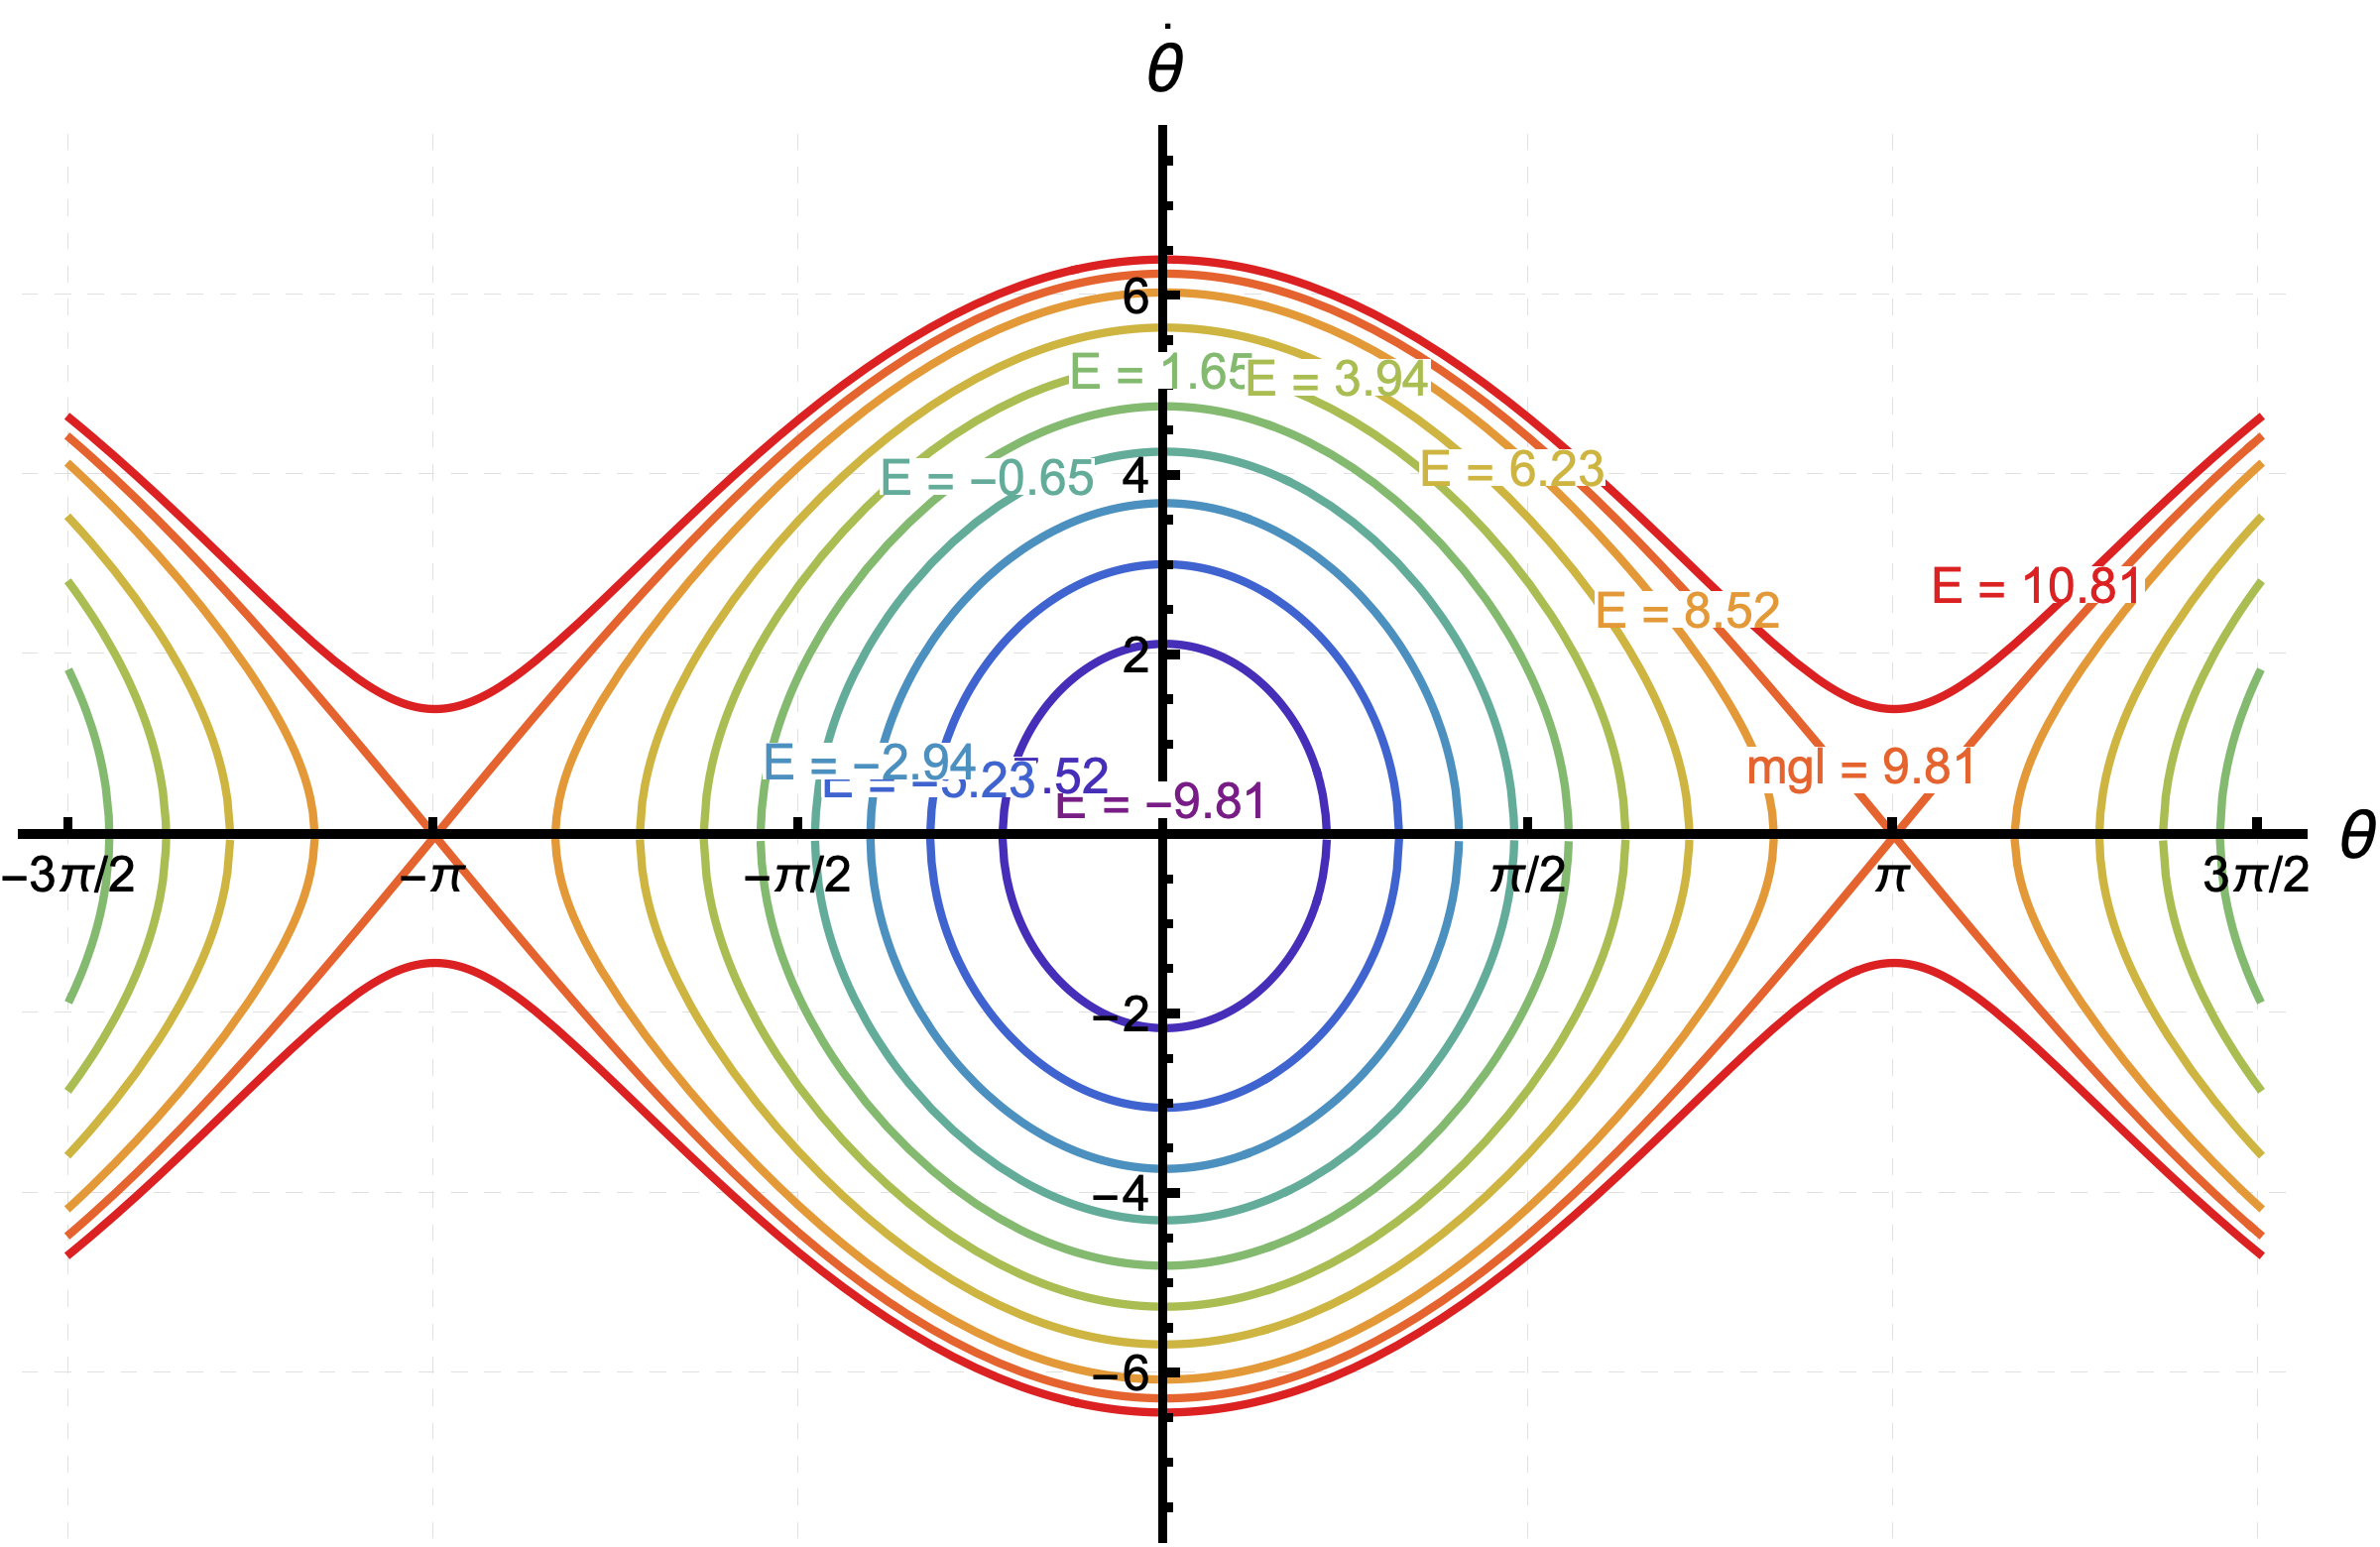
\includegraphics[scale=0.6]{immagini/grafico_pendolo.png}
\end{center}

Si può notare che se il livello energetico è basso sono permessi solo stati con
\(\theta\) piccola e che, assieme a \(\dot{\theta}\), siano confinati tra un
valore minimo e uno massimo, cioè curve chiuse.

Questo corrisponde a far oscillare il pendolo con un angolo massimo inferiore
a \(\pi\).

Per
\[
\theta=\pi,
\qquad
\dot{\theta}=0,
\]
si ha
\[
E=mg\ell
\]
e quindi
\[
1=
\frac{m\ell^2}{4mg}\dot{\theta}^{\,2}
-
\frac{(\theta-\pi)^2}{4}.
\]

È l'iperbole degenere gialla con centro \(\theta=\pi\).
\(\theta=\pi\) è l'angolo minimo per cui le curve si aprono. Vedremo come
questo è legato alla stabilità degli stati di equilibrio.

Nel piano delle fasi, per
\[
\theta\ll 1,
\]
la curva del moto del pendolo è molto simile a quella dell'oscillatore
armonico. Proviamo a caratterizzare in modo analitico quanto simile.

Oscillatore armonico:
\[
m\ddot{x}=-kx.
\]

Pendolo:
\[
m\ell^2\ddot{\theta}
=
-mg\ell\sin\theta.
\]
Per
\[
\theta\ll 1
\]
si ha
\[
\sin\theta\simeq \theta,
\]
quindi
\[
m\ell^2\ddot{\theta}
=
-mg\ell\theta.
\]

Di conseguenza
\[
\left\{
\begin{array}{l}
\theta(t)=A\cos(\omega t+\varphi),\\[1mm]
\dot{\theta}(t)=-A\omega\sin(\omega t+\varphi),
\end{array}
\right.
\qquad
\omega=\sqrt{\dfrac{g}{\ell}}.
\]

Ovvero, per
\[
\theta\ll 1,
\]
il moto è esattamente un moto armonico.

Si dimostra facilmente che le configurazioni di equilibrio del pendolo sono
\[
\theta_1=0,
\qquad
\theta_2=\pi.
\]
\end{example}



\section{Stabilità delle configurazioni di equilibrio}

Consideriamo un sistema ad un grado di libertà definito dalla coordinata libera
\[
q(t).
\]
All'equilibrio si ha
\[
\underline{f}\cdot \delta\underline{x}
=
\underline{f}\cdot
\frac{\partial \underline{x}}{\partial q}\,\delta q
=
0
\qquad \Longrightarrow \qquad
\underline{f}\cdot
\frac{\partial \underline{x}}{\partial q}
=
0.
\]

Ottengo una configurazione \(\hat{q}\). Vogliamo caratterizzare la
stabilità di questa configurazione.

\begin{example}{}[Pendolo]
Consideriamo il pendolo classico. Poniamo
\[
q=\theta.
\]
Le configurazioni di equilibrio sono
\[
\theta_1=0,
\qquad
\theta_2=\pi.
\]


Euristicamente, \(\theta=0\) è una configurazione d'equilibrio stabile perché,
se ho una condizione iniziale del moto ``vicina'', nel moto resta ``vicina'' a
\(\theta=0\).

Se invece \(\theta=\pi\), è una configurazione di equilibrio instabile perché,
se ho una condizione iniziale del moto ``vicina'', nel moto si allontana da
\(\theta=\pi\).
\end{example}

Formalmente diamo la seguente definizione di \textbf{stabilità}.
\begin{definition}{}
Sia \(\underline{q}(t)\) il moto di un sistema meccanico e sia \(\hat{\underline{q}}\) una configurazione di equilibrio.

La configurazione \(\hat{\underline{q}}\) è di equilibrio stabile se
\[
\forall \varepsilon>0\ \exists \delta>0
\]
tale che, per ogni \(\underline{q}\),
\[
\left|\hat{\underline{q}}-\underline{q}(0)\right|<\delta,
\qquad
\left|\dot{\underline{q}}(0)\right|<\delta
\ \Longrightarrow\
\left|\underline{q}(t)-\hat{\underline{q}}\right|<\varepsilon
\qquad \forall t>0.
\]
\end{definition}
Se
\[
\underline{q}=(q_1,q_2),
\]
si può visualizzare la definizione nel seguente modo:

\begin{center}
\begin{tikzpicture}[x=1cm,y=1cm,>=Latex]
    % assi
    \draw[->, line width=0.9pt] (0,0) -- (5.7,0) node[right] {$q_1$};
    \draw[->, line width=0.9pt] (0,0) -- (0,4.1) node[above] {$q_2$};

    % centro
    \coordinate (Q) at (3.2,2.2);
    \fill (Q) circle (1.2pt);

    % tacche sugli assi
    \draw[line width=0.8pt] (3.2,-0.08) -- (3.2,0.08);
    \draw[line width=0.8pt] (-0.08,2.2) -- (0.08,2.2);

    % etichette assi corrispondenti
    \node[below] at (3.2,-0.1) {$\hat{q}_1$};
    \node[left] at (-0.05,2.2) {$\hat{q}_2$};

    % palle
    \draw[red, dashed, line width=0.9pt] (Q) circle (0.65);
    \draw[green!60!black, dashed, line width=0.9pt] (Q) circle (1.15);

    % freccia delta
    \draw[->, red, line width=0.9pt] (Q) -- ++(135:0.65);
    \node[red, above left] at ($(Q)+(135:0.38)$) {$\delta$};

    % freccia epsilon
    \draw[->, green!60!black, line width=0.9pt] (Q) -- ++(-35:1.15);
    \node[green!60!black, right] at ($(Q)+(-35:0.72)$) {$\varepsilon$};

    % etichetta centro
    \node[right] at ($(Q)+(0.12,0.08)$) {$\hat{\underline{q}}$};
\end{tikzpicture}
\end{center}

Se
\[
\underline{q}(0)\in B_\delta(\hat{\underline{q}})
\quad\Longrightarrow\quad
\underline{q}(t)\in B_\varepsilon(\hat{\underline{q}})
\qquad \forall t>0.
\]



La definizione di configurazione di equilibrio stabile è complicata da usare
nella pratica. Ma per forze conservative vale il teorema di Dirichlet.

\begin{theorem}{}[Dirichlet]
Se \(\hat{\underline{q}}\) è un minimo locale stretto di \(V(\underline{q})\),
allora \(\hat{\underline{q}}\) è una configurazione d'equilibrio stabile per il
sistema.
\end{theorem}

\begin{proof}
Sia
\[
E(\underline{q},\dot{\underline{q}})
=
T(\underline{q} , \dot{\underline{q}})+V(\underline{q})
\]
l'energia totale del sistema. Poiché il sistema è conservativo si ha che
\[
E(\underline{q}(t),\dot{\underline{q}}(t))=\text{cost.}
\qquad \forall t.
\]

Inoltre
\[
T(\underline{q} , \dot{\underline{q}})\geq 0,
\qquad
T(\underline{q} , \dot{\underline{q}})=0
\Longleftrightarrow
\dot{\underline{q}}=\underline{0}.
\]

Poiché \(\hat{\underline{q}}\) è un minimo locale stretto di \(V\),
fissato \(\varepsilon\) sufficientemente piccolo, si ha che
\[
\forall \underline{q}\in \partial B_\varepsilon
(\hat{\underline{q}})
\qquad
V(\underline{q})>V(\hat{\underline{q}}).
\]

Inoltre \(\partial B_\varepsilon(\hat{\underline{q}})\) è un compatto e
la funzione
\[
V(\underline{q})-V(\hat{\underline{q}})
\]
è continua su \(\partial B_\varepsilon(\hat{\underline{q}})\) ed inoltre
strettamente positiva. Per il teorema di Weierstrass ammette minimo
\(m_\varepsilon>0\). Allora
\[
\forall \underline{q}\in \partial B_\varepsilon(\hat{\underline{q}})
\qquad
V(\underline{q})-V(\hat{\underline{q}})\geq m_\varepsilon
\]
cioè
\[
V(\underline{q})\geq m_\varepsilon+V(\hat{\underline{q}}).
\]

Abbiamo trovato che su \(\partial B_\varepsilon(\hat{\underline{q}})\)
\(V\) non può scendere al di sotto del valore di \(V\) in
\(\hat{\underline{q}}\) maggiorato di una costante positiva.

Ricordiamo ora che
\[
E(\underline{q},\dot{\underline{q}})
\]
è continua e in particolare lo è in
\[
(\hat{\underline{q}},\underline{0}),
\]
punto di equilibrio. Allora, fissato \(m_\varepsilon>0\) come sopra,
\[
\exists \ell>0
\]
tale che
\[
\left|
(\hat{\underline{q}},\underline{0})
-
(\underline{q}(0),\dot{\underline{q}}(0))
\right|<\ell
\]
implica
\[
\left|
E(\underline{q}(0),\dot{\underline{q}}(0))
-
E(\hat{\underline{q}},\underline{0})
\right|
=
\left|
E(\underline{q}(0),\dot{\underline{q}}(0))
-
V(\hat{\underline{q}})
\right|
<m_\varepsilon.
\]

Possiamo ripartire la distanza da
\[
(\hat{\underline{q}},\underline{0})
\]
sulle \(2\) componenti e dire che
\[
\exists \delta^*>0
\]
tale che
\[
|\hat{\underline{q}}-\underline{q}(0)|<\delta^*,
\qquad
|\dot{\underline{q}}(0)|<\delta^*
\]
implica
\[
\left|
E(\underline{q}(0),\dot{\underline{q}}(0))
-
V(\hat{\underline{q}})
\right|
<m_\varepsilon.
\]
Quindi
\[
E(\underline{q}(0),\dot{\underline{q}}(0))
<
m_\varepsilon+V(\hat{\underline{q}}).
\]

La condizione vale anche per
\[
\delta=\min\{\delta^*,\varepsilon\}.
\]

Considero quindi \(\underline{q}(t)\) tale che
\[
|\underline{q}(0)-\hat{\underline{q}}|<\delta,
\qquad
|\dot{\underline{q}}(0)|<\delta,
\]
ovvero ci siamo messi in una situazione iniziale con energia totale minore
dell'energia potenziale minima su
\(\partial B_\varepsilon(\hat{\underline{q}})\) e con posizione iniziale
\[
\underline{q}(0)\in B_\varepsilon(\hat{\underline{q}}).
\]

Supponiamo per assurdo che esista un istante \(t_1\geq 0\) tale che
\[
\underline{q}(t_1)\notin B_\varepsilon(\hat{\underline{q}}),
\]
ovvero
\[
|\underline{q}(t_1)-\hat{\underline{q}}|\geq \varepsilon.
\]

Per continuità di \(\underline{q}(t)\) deve esistere
\[
0\leq t^*\leq t_1
\]
tale che
\[
\underline{q}(t^*)\in \partial B_\varepsilon(\hat{\underline{q}}).
\]

Analizziamo il bilancio energetico all'istante \(t^*\):
\[
E(\underline{q}(t^*),\dot{\underline{q}}(t^*))
=
T(\dot{\underline{q}}(t^*))
+
V(\underline{q}(t^*))
\geq
V(\hat{\underline{q}})+m_\varepsilon
+
T(\dot{\underline{q}}(t^*))
\geq
V(\hat{\underline{q}})+m_\varepsilon.
\]

D'altra parte
\[
E(\underline{q}(t^*),\dot{\underline{q}}(t^*))
<
m_\varepsilon+V(\hat{\underline{q}}).
\]

Abbiamo trovato che
\[
E(\underline{q}(t^*),\dot{\underline{q}}(t^*))
\]
deve essere maggiore o uguale e minore di una quantità, che è un assurdo.

Allora
\[
|\underline{q}(0)-\hat{\underline{q}}|<\delta,
\qquad
|\dot{\underline{q}}(0)|<\delta
\]
implica
\[
|\underline{q}(t)-\hat{\underline{q}}|<\varepsilon
\qquad
\forall t>0.
\]
Ovvero \(\hat{\underline{q}}\) è stabile.
\end{proof}

Possiamo quindi individuare i punti di equilibrio risolvendo $\nabla V(\underline{q}) = 0$ e caratterizzando la loro stabilità studiando il segno degli autovalori della matrice hessiana $H_V(\underline{q})$.
\begin{example}{}
    Riconsideriamo l'esempio dello scorso capitolo con le stesse ipotesi e studiamo la stabilità delle configurazioni di equilibrio.

    \begin{center}
    \begin{tikzpicture}[
    x=1cm,
    y=1cm,
    >=Latex,
    line cap=round,
    line join=round,
    every node/.style={font=\small}
]

% Parametri
\def\R{1.55}

% Coordinate
\coordinate (O) at (0,0);
\coordinate (A) at (0,3.45);
\coordinate (G) at (7.20,\R);
\coordinate (C) at (7.20,0);
\coordinate (Top) at ($(G)+(0,\R)$);
\coordinate (B) at ($(A)!0.42!(G)$);

% Assi
\draw[black, line width=1.4pt, ->] (0,0) -- (10.2,0) node[below right] {$x$};
\draw[black, line width=1.4pt, ->] (0,0) -- (0,4.2) node[above left] {$y$};

% Parete verticale
\draw[black, line width=2pt] (0,0) -- (0,4.05);

% Origine
\node[below left] at (O) {$O$};

% Riferimento centrato in O
\draw[orange!85!black, line width=1.4pt, ->] (O) -- ++(0.95,0);
\draw[orange!85!black, line width=1.4pt, ->] (O) -- ++(0,0.95);
\node[orange!85!black, below] at ($(O)+(0.48,0)$) {$\underline{\imath}$};
\node[orange!85!black, left] at ($(O)+(0,0.48)$) {$\underline{\jmath}$};

\draw[orange!85!black, line width=1.2pt] (-0.45,0.18) circle (0.18);
\fill[orange!85!black] (-0.45,0.18) circle (0.03);
\node[orange!85!black, left] at (-0.62,0.62) {$\underline{k}$};

% Sbarrette verticali attaccate all'asse y
\draw[black, line width=1.6pt] (0,3.14) -- (0,3.56);
\draw[black, line width=1.6pt] (0.12,3.14) -- (0.12,3.56);

% Punto A
\node[left] at (A) {$A$};

% Asta
\draw[black, line width=1.8pt] (A) -- (G);

% Punto B
\fill[red] (B) circle (2.8pt);
\node[above] at (B) {$B$};

% Etichetta asta
\node[above right] at ($(B)!0.52!(G)$) {$l,m$};

% Angolo theta
\draw[black, line width=1.1pt]
($(A)+(0,-0.78)$) arc[start angle=-90,end angle=-14.5,radius=0.78];
\node at ($(A)+(0.72,-0.87)$) {$\theta$};

% Freccia verde in A
\draw[green!55!black, line width=1.4pt, ->] ($(A)$) -- ++(1.80,0);
\node[green!55!black, above] at ($(A)+(1.25,0.20)$) {$\underline{\psi}$};

% Molla attaccata all'asse y
\draw[black, line width=1.4pt, smooth, samples=240, domain=0:7.02]
plot (\x,{1.55 + 0.10*sin(900*\x)});

% Ruota
\draw[black, line width=1.8pt] (G) circle (\R);

% Punto C
\node[below] at (C) {$C$};

% Centro G
\filldraw[white, draw=black, line width=1.2pt] (G) circle (0.09);
\node[above left] at ($(G)+(-0.10,0.08)$) {$G$};

% Etichetta M,R
\node[above right] at ($(Top)+(0.95,-0.05)$) {$M,R$};

% Raggi tratteggiati
\draw[black, dashed, line width=1.1pt] (Top) -- (G);
\draw[black, dashed, line width=1.1pt] (G) -- ++(0.95,1.00);

% Angolo phi
\draw[black, line width=1.0pt, ->]
($(G)+(0,0.58)$) arc[start angle=90,end angle=46,radius=0.58];
\node at ($(G)+(0.47,0.92)$) {$\varphi$};

% Forza mg in B
\draw[red!85!black, line width=1.5pt, ->] (B) -- ++(0,-1.15);
\node[red!85!black, left] at ($(B)+(0.10,-0.70)$) {$m\underline{g}$};

% Forza Mg in G
\draw[red!85!black, line width=1.5pt, ->] (G) -- ++(0,-1.05);
\node[red!85!black, right] at ($(G)+(0.52,-0.62)$) {$M\underline{g}$};

% Forza elastica
\draw[red!85!black, line width=1.5pt, ->] (G) -- ++(-1.25,0);
\node[red!85!black, below] at ($(G)+(-0.82,-0.12)$) {$-k\,\underline{x}_G$};

% Assi verdi vicino a C
\draw[green!55!black, line width=1.4pt, ->] ($(C)+(0.18,0)$) -- ++(1.90,0);
\draw[green!55!black, line width=1.4pt, ->] ($(C)+(0.18,0)$) -- ++(0,0.95);
\node[green!55!black, right] at ($(C)+(2.10,0)$) {$\underline{\xi}_x$};
\node[green!55!black, right] at ($(C)+(0.22,0.58)$) {$\underline{\xi}_y$};

\end{tikzpicture}
  \end{center}


  Studiamo la stabilità delle configurazioni d'equilibrio. Il potenziale
\(V(\theta)\) è
\[
V
=
\frac{kx_G^2}{2}
+
mg\left(R+\frac{\ell}{2}\cos\theta\right)
+
MgR
=
\frac{k}{2}\ell^2\sin^2\theta
+
mg\left(R+\frac{\ell}{2}\cos\theta\right)
+
MgR.
\]

Allora
\[
\nabla V
=
\frac{dV}{d\theta}
=
2\frac{k}{2}\ell^2\sin\theta\cos\theta
-
mg\frac{\ell}{2}\sin\theta
=
0,
\]
cioè
\[
k\ell^2\sin\theta\cos\theta
-
mg\frac{\ell}{2}\sin\theta
=
0.
\]

Quindi
\[
\theta_1=0,
\qquad
\theta_2=\pi,
\qquad
\cos\theta_{3,4}
=
\frac{mg}{2k\ell}
\quad
\text{se}
\quad
\frac{mg}{2k\ell}\leq 1.
\]

Sono le configurazioni d'equilibrio.

Calcoliamo la derivata seconda, cioè l'hessiana:
\[
\frac{d^2V}{d\theta^2}
=
k\ell^2\cos^2\theta
-
k\ell^2\sin^2\theta
-
mg\frac{\ell}{2}\cos\theta.
\]

Valuto nelle configurazioni di equilibrio:
\[
\frac{d^2V}{d\theta^2}(0)
=
k\ell^2
-
mg\frac{\ell}{2}.
\]
Quindi è stabile se
\[
k\ell^2>mg\frac{\ell}{2}
\Longleftrightarrow
2k\ell>mg
\Longleftrightarrow
1>\frac{mg}{2k\ell}.
\]

Inoltre
\[
\frac{d^2V}{d\theta^2}(\pi)
=
k\ell^2
+
mg\frac{\ell}{2}
>
0,
\]
quindi è sempre stabile.

Infine
\[
\left.
\frac{d^2V}{d\theta^2}(\theta_3,\theta_4)
=
k\ell^2\cos^2\theta
-
k\ell^2(1-\cos^2\theta)
-
mg\frac{\ell}{2}\cos\theta
\right|_{\theta_3,\theta_4}
\]
\[
=
\frac{(mg)^2}{4k}
-
k\ell^2
>
0.
\]
Dunque
\[
(mg)^2>4k^2\ell^2
\Longleftrightarrow
mg>2k\ell
\Longleftrightarrow
1<
\frac{mg}{2k\ell}.
\]









  \begin{center}
  \begin{tikzpicture}[scale=1, line cap=round, line join=round, >=Latex]

%======================
% Disegno 1
%======================
\begin{scope}[shift={(0,0)}]
    \node at (0,3.35) {$\theta_1=0$};

    % piano
    \draw[line width=0.9pt] (-1.7,0) -- (1.7,0);

    % disco
    \draw[line width=1pt] (0,1) circle (1);

    % asta verticale
    \draw[line width=1pt] (0,1) -- (0,2.85);

    % punto A e guida
    \fill (0,2.15) circle (1.2pt);
    \node[right] at (0,2.15) {$A$};
    \draw[line width=0.8pt] (-0.13,1.90) -- (-0.13,2.40);
    \draw[line width=0.8pt] ( 0.13,1.90) -- ( 0.13,2.40);
\end{scope}

%======================
% Disegno 2
%======================
\begin{scope}[shift={(5.6,0)}]
    \node at (0,3.35) {$\theta_2=\pi$};

    % piano
    \draw[line width=0.9pt] (-1.7,0) -- (1.7,0);

    % disco
    \draw[line width=1pt] (0,1) circle (1);

    % asta verticale verso il basso
    \draw[line width=1pt] (0,1) -- (0,-1.05);

    % punto A e guida
    \fill (0,-0.38) circle (1.2pt);
    \node[right] at (0,-0.38) {$A$};
    \draw[line width=0.8pt] (-0.13,-0.63) -- (-0.13,-0.13);
    \draw[line width=0.8pt] ( 0.13,-0.63) -- ( 0.13,-0.13);
\end{scope}

%======================
% Disegno 3
%======================
\begin{scope}[shift={(12.4,0)}]
    \node at (0,3.35) {$\theta_3,\theta_4$};

    % piano con freccia
    \draw[line width=0.9pt, ->] (-3.3,0) -- (4.2,0);

    % asse verticale centrale
    \draw[line width=1pt] (0,-1.4) -- (0,2.95);

    % dischi
    \draw[line width=1pt] (-1.7,1) circle (1);
    \draw[line width=1pt] ( 1.7,1) circle (1);

    % centri dei dischi
    \coordinate (GL) at (-1.7,1);
    \coordinate (GR) at ( 1.7,1);
    \coordinate (A)  at (0,2.18);

    % punto A e guida
    \fill (A) circle (1.2pt);
    \node[right] at (A) {$A$};
    \draw[line width=0.8pt] (-0.13,1.92) -- (-0.13,2.42);
    \draw[line width=0.8pt] ( 0.13,1.92) -- ( 0.13,2.42);

    % aste inclinate che partono dai centri delle circonferenze
    \draw[line width=1pt] (GL) -- (A);
    \draw[line width=1pt] (GR) -- (A);

    % molla orizzontale tra i due centri
    \draw[line width=1pt] (-1.7,1) -- (-1.25,1);

    \draw[line width=1pt, smooth, samples=100, domain=-1.25:-0.15]
        plot (\x,{1 + 0.07*sin((\x+1.25)/1.10*1080)});

    \fill (0,1) circle (1.2pt);

    \draw[line width=1pt, smooth, samples=100, domain=0.15:1.25]
        plot (\x,{1 + 0.07*sin((\x-0.15)/1.10*1080)});

    \draw[line width=1pt] (1.25,1) -- (1.7,1);
\end{scope}

\end{tikzpicture}
\end{center}


\[
\begin{array}{ll}
\bullet & \theta_1=0
\quad \text{esiste sempre ed è stabile per }
\dfrac{mg}{2k\ell}<1,
\\[4mm]
\bullet & \theta_2=\pi
\quad \text{esiste ed è stabile sempre},
\\[4mm]
\bullet & \theta_3,\theta_4
\quad \text{esistono per }
\dfrac{mg}{2k\ell}\leq 1
\quad \text{e sono stabili per }
\dfrac{mg}{2k\ell}>1.
\end{array}
\]

Ovvero:
\[
\begin{array}{ll}
\bullet &
\dfrac{mg}{2k\ell}>1
\quad \Longrightarrow \quad
\exists\,\theta_1,\theta_2,
\\[3mm]
&
\theta_1 \text{ instabile},
\qquad
\theta_2 \text{ stabile};
\\[6mm]
\bullet &
\dfrac{mg}{2k\ell}<1
\quad \Longrightarrow \quad
\exists\,\theta_1,\theta_2,\theta_3,\theta_4,
\\[3mm]
&
\theta_1 \text{ stabile},
\qquad
\theta_2 \text{ stabile},
\\[2mm]
&
\theta_3,\theta_4 \text{ instabili}.
\end{array}
\]
\end{example}

\chapter{Equazioni di Eulero-Lagrange e integrali primi del moto}

\section{Equazioni di Eulero-Lagrange}
\begin{lemma}{}
Consideriamo $n$ punti materiali $\underline{x}_1, \underline{x}_2, \ldots, \underline{x}_n$ soggetti a $3n - m$ vincoli olonomi. Supponiamo che il sistema sia rappresentato da $m$ coordinate libere $q_1(t), \ldots, q_m(t)$. Allora vale la relazione
\[
\frac{\partial \dot{\underline{x}}_i}{\partial \dot{q}_j}
=
\frac{\partial \underline{x}_i}{\partial q_j}
\qquad
\forall i = 1,\ldots,n,\quad \forall j = 1,\ldots,m .
\]
\end{lemma}
\begin{proof}
Ricordiamo che $\underline{x}_i(q_1,\ldots,q_m,t)$ dipende dalle coordinate libere ma non dalle loro derivate temporali, allora
\[
\frac{\partial \underline{x}_i}{\partial \dot{q}_j} = 0
\qquad \forall j = 1,\ldots,m .
\]

Quindi
\[
\frac{\partial \dot{\underline{x}}_i}{\partial \dot{q}_j}
=
\frac{\partial}{\partial \dot{q}_j}
\frac{d\underline{x}_i}{dt}
=
\frac{\partial}{\partial \dot{q}_j}
\sum_k
\frac{\partial \underline{x}_i}{\partial q_k}
\frac{dq_k}{dt}
=
\frac{\partial}{\partial \dot{q}_j}
\sum_k
\frac{\partial \underline{x}_i}{\partial q_k}
\dot{q}_k
\]
\[
=
\sum_k
\frac{\partial \underline{x}_i}{\partial q_k}
\frac{\partial \dot{q}_k}{\partial \dot{q}_j}
=
\sum_k
\frac{\partial \underline{x}_i}{\partial q_k}
\delta_{kj}
=
\frac{\partial \underline{x}_i}{\partial q_j}.
\]
\end{proof}

Scriviamo il principio dei lavori virtuali per il sistema descritto nel lemma aggiungendo il termine d'inerzia:
\[
\sum_{i=1}^{n} m_i \ddot{\underline{x}}_i \cdot \delta \underline{x}_i
=
\sum_{i=1}^{n} \underline{f}_i \cdot \delta \underline{x}_i
\qquad
\forall \left(\delta \underline{x}_1,\ldots,\delta \underline{x}_n\right).
\]

Dove $\delta \underline{x}_i$ è uno spostamento virtuale ammesso dai vincoli perfetti e olonomi per il punto $\underline{x}_i$. Come abbiamo già fatto in precedenza possiamo scrivere
\[
\sum_{i=1}^{n} \underline{f}_i \cdot \delta \underline{x}_i
=
\sum_{i=1}^{n} \underline{f}_i^{\mathrm{ATT}} \cdot \delta \underline{x}_i
=
\sum_{i=1}^{n} \underline{f}_i^{\mathrm{ATT}} \cdot
\sum_{j=1}^{m}
\frac{\partial \underline{x}_i}{\partial q_j}\delta q_j
=
\sum_{j=1}^{m}
\left(
\sum_{i=1}^{n}
\underline{f}_i^{\mathrm{ATT}} \cdot
\frac{\partial \underline{x}_i}{\partial q_j}
\right)\delta q_j
=
\sum_{j=1}^{m} Q_j \delta q_j.
\]

Inoltre
\[
\sum_{i=1}^{n} m_i \ddot{\underline{x}}_i \cdot \delta \underline{x}_i
=
\sum_{i=1}^{n} m_i \ddot{\underline{x}}_i \cdot
\sum_{j=1}^{m}
\frac{\partial \underline{x}_i}{\partial q_j}\delta q_j
=
\sum_{j=1}^{m}
\left(
\sum_{i=1}^{n}
m_i \ddot{\underline{x}}_i \cdot
\frac{\partial \underline{x}_i}{\partial q_j}
\right)\delta q_j.
\]

Ricordiamo che
\[
\left(\frac{d}{dt}f\right)\cdot g
=
\frac{d}{dt}(f\cdot g)
-
f\cdot \frac{d}{dt}(g).
\]
Allora
\[
\sum_{j=1}^{m}
\left(
\sum_{i=1}^{n}
m_i \ddot{\underline{x}}_i \cdot
\frac{\partial \underline{x}_i}{\partial q_j}
\right)\delta q_j
=
\sum_{j=1}^{m}
\left(
\sum_{i=1}^{n}
\left[
\frac{d}{dt}
\left(
m_i \dot{\underline{x}}_i \cdot
\frac{\partial \underline{x}_i}{\partial q_j}
\right)
-
m_i \dot{\underline{x}}_i \cdot
\frac{d}{dt}
\left(
\frac{\partial \underline{x}_i}{\partial q_j}
\right)
\right]
\right)\delta q_j.
\]

Ora applichiamo il lemma al primo
$
{\partial \underline{x}_i}/{\partial q_j}.
$

\[
\sum_{j=1}^{m}\sum_{i=1}^{n}
\left[
\frac{d}{dt}
\left(
m_i \dot{\underline{x}}_i \cdot
\frac{\partial \underline{ \dot x}_i}{\partial \dot q_j}
\right)
-
m_i \dot{\underline{x}}_i \cdot
\frac{\partial \dot{\underline{x}}_i}{\partial q_j}
\right]\delta q_j
=
\]
\[
=
\sum_{j=1}^{m}\sum_{i=1}^{n}
\left[
\frac{d}{dt}
\left(
m_i \underline{v}_i \cdot
\frac{\partial \underline{v}_i}{\partial \dot{q}_j}
\right)
-
m_i \underline{v}_i \cdot
\frac{\partial \underline{v}_i}{\partial q_j}
\right]\delta q_j
=
\]
\[
=
\sum_{j=1}^{m}
\left[
\frac{d}{dt}
\left(
\sum_{i=1}^{n}
m_i \underline{v}_i \cdot
\frac{\partial \underline{v}_i}{\partial \dot{q}_j}
\right)
-
\sum_{i=1}^{n}
m_i \underline{v}_i \cdot
\frac{\partial \underline{v}_i}{\partial q_j}
\right]\delta q_j
=
\]
\[
=
\sum_{j=1}^{m}
\left[
\frac{d}{dt}
\left(
\frac{\partial}{\partial \dot{q}_j}
\sum_{i=1}^{n}
m_i \frac{\underline{v}_i \cdot \underline{v}_i}{2}
\right)
-
\frac{\partial}{\partial q_j}
\left(
\sum_{i=1}^{n}
m_i \frac{\underline{v}_i \cdot \underline{v}_i}{2}
\right)
\right]\delta q_j
=
\]
\[
=
\sum_{j=1}^{m}
\left[
\frac{d}{dt}
\frac{\partial T}{\partial \dot{q}_j}
-
\frac{\partial T}{\partial q_j}
\right]\delta q_j.
\]

Mettendo assieme i due membri otteniamo
\[
\sum_{j=1}^{m}
\left[
\frac{d}{dt}
\frac{\partial T}{\partial \dot{q}_j}
-
\frac{\partial T}{\partial q_j}
\right]\delta q_j
=
\sum_{j=1}^{m} Q_j \delta q_j
\qquad
\forall (\delta q_1,\ldots,\delta q_m).
\]

\[
\Rightarrow \sum_{j=1}^{m}
\left[
\frac{d}{dt}
\frac{\partial T}{\partial \dot{q}_j}
-
\frac{\partial T}{\partial q_j}
-
Q_j
\right]\delta q_j
=
0
\qquad
\forall (\delta q_1,\ldots,\delta q_m).
\]

\[
\Rightarrow \begin{pmatrix}
\frac{d}{dt}\frac{\partial T}{\partial \dot{q}_1}
-
\frac{\partial T}{\partial q_1}
-
Q_1
\\
\vdots
\\
\frac{d}{dt}\frac{\partial T}{\partial \dot{q}_m}
-
\frac{\partial T}{\partial q_m}
-
Q_m
\end{pmatrix}
\cdot
\begin{pmatrix}
\delta q_1
\\
\vdots
\\
\delta q_m
\end{pmatrix}
=
0
\qquad
\forall (\delta q_1,\ldots,\delta q_m).
\]

\[
\Rightarrow \frac{d}{dt}
\frac{\partial T}{\partial \dot{q}_j}
-
\frac{\partial T}{\partial q_j}
-
Q_j
=
0
\qquad
\forall j = 1,\ldots,m.
\]

\[
\Rightarrow \frac{d}{dt}
\frac{\partial T}{\partial \dot{q}_j}
-
\frac{\partial T}{\partial q_j}
=
Q_j
\qquad
\forall j = 1,\ldots,m.
\]
Chiamiamo queste ultime equazioni \textbf{equazioni di Eulero-Lagrange} o più semplicemente \textbf{equazioni di Lagrange}. Le \textbf{equazioni di Lagrange} sono $m$ equazioni (per un sistema con $m$ gradi di libertà) del $II$ ordine nel tempo. Nelle equazioni non compaiono le reazioni vincolari.

Consideriamo ora un sistema sul quale agiscono solo forze conservative:
\[
Q_j
=
\sum_{i=1}^{n}
\underline{f}_i^{\mathrm{ATT}}
\cdot
\frac{\partial \underline{x}_i}{\partial q_j}
=
\sum_{i=1}^{n}
-\nabla V_i
\cdot
\frac{\partial \underline{x}_i}{\partial q_j}
=
\sum_{i=1}^{n}
-
\begin{pmatrix}
\frac{\partial V_i}{\partial x_i}
\\[2pt]
\frac{\partial V_i}{\partial y_i}
\\[2pt]
\frac{\partial V_i}{\partial z_i}
\end{pmatrix}
\cdot
\frac{\partial \underline{x}_i}{\partial q_j}
=
\]
\[
=
\sum_{i=1}^{n}
-
\frac{\partial V_i}{\partial q_j}
=
-
\frac{\partial V}{\partial q_j}.
\]

Allora
\[
\frac{d}{dt}
\frac{\partial T}{\partial \dot{q}_j}
-
\frac{\partial T}{\partial q_j}
=
-
\frac{\partial V}{\partial q_j}
\quad \Longrightarrow \quad
\frac{d}{dt}
\frac{\partial T}{\partial \dot{q}_j}
-
\frac{\partial}{\partial q_j}
(T - V)
=
0.
\]

Dal momento che
\[
\frac{\partial V}{\partial \dot{q}_j} = 0
\]
possiamo scrivere
\[
\frac{d}{dt}
\frac{\partial}{\partial \dot{q}_j}
(T - V)
-
\frac{\partial}{\partial q_j}
(T - V)
=
0.
\]

Chiamiamo ora funzione lagrangiana la funzione
\[
\mathcal{L}(\underline{q},\dot{\underline{q}})
=
T(\underline{q},\dot{\underline{q}})
-
V(\underline{q}).
\]

Otteniamo infine
\[
\frac{d}{dt}
\frac{\partial \mathcal{L}}{\partial \dot{q}_j}
-
\frac{\partial \mathcal{L}}{\partial q_j}
=
0. \quad \forall j = 1, \ldots , m
\]

ovvero le \textbf{equazioni di Lagrange per sistemi conservativi}.



\begin{example}{}
Vogliamo studiare la dinamica del sistema in figura. Farlo attraverso le equazioni cardinali è molto complesso. Dal momento che agiscono solo forze conservative, può essere vantaggioso usare le equazioni di Lagrange.
\begin{center}
    \begin{tikzpicture}[
    x=1cm,
    y=1cm,
    >=Latex,
    line cap=round,
    line join=round,
    every node/.style={font=\small}
]

% Parametri
\def\R{1.55}

% Coordinate
\coordinate (O) at (0,0);
\coordinate (A) at (0,3.45);
\coordinate (G) at (7.20,\R);
\coordinate (C) at (7.20,0);
\coordinate (Top) at ($(G)+(0,\R)$);
\coordinate (B) at ($(A)!0.42!(G)$);

% Assi
\draw[black, line width=1.4pt, ->] (0,0) -- (10.2,0) node[below right] {$x$};
\draw[black, line width=1.4pt, ->] (0,0) -- (0,4.2) node[above left] {$y$};

% Parete verticale
\draw[black, line width=2pt] (0,0) -- (0,4.05);

% Origine
\node[below left] at (O) {$O$};

% Riferimento centrato in O
\draw[orange!85!black, line width=1.4pt, ->] (O) -- ++(0.95,0);
\draw[orange!85!black, line width=1.4pt, ->] (O) -- ++(0,0.95);
\node[orange!85!black, below] at ($(O)+(0.48,0)$) {$\underline{\imath}$};
\node[orange!85!black, left] at ($(O)+(0,0.48)$) {$\underline{\jmath}$};

\draw[orange!85!black, line width=1.2pt] (-0.45,0.18) circle (0.18);
\fill[orange!85!black] (-0.45,0.18) circle (0.03);
\node[orange!85!black, left] at (-0.62,0.62) {$\underline{k}$};

% Sbarrette verticali attaccate all'asse y
\draw[black, line width=1.6pt] (0,3.14) -- (0,3.56);
\draw[black, line width=1.6pt] (0.12,3.14) -- (0.12,3.56);

% Punto A
\node[left] at (A) {$A$};

% Asta
\draw[black, line width=1.8pt] (A) -- (G);

% Punto B
\fill[red] (B) circle (2.8pt);
\node[above] at (B) {$B$};

% Etichetta asta
\node[above right] at ($(B)!0.52!(G)$) {$l,m$};

% Angolo theta
\draw[black, line width=1.1pt]
($(A)+(0,-0.78)$) arc[start angle=-90,end angle=-14.5,radius=0.78];
\node at ($(A)+(0.72,-0.87)$) {$\theta$};

% Freccia verde in A
\draw[green!55!black, line width=1.4pt, ->] ($(A)$) -- ++(1.80,0);
\node[green!55!black, above] at ($(A)+(1.25,0.20)$) {$\underline{\psi}$};

% Molla attaccata all'asse y
\draw[black, line width=1.4pt, smooth, samples=240, domain=0:7.02]
plot (\x,{1.55 + 0.10*sin(900*\x)});

% Ruota
\draw[black, line width=1.8pt] (G) circle (\R);

% Punto C
\node[below] at (C) {$C$};

% Centro G
\filldraw[white, draw=black, line width=1.2pt] (G) circle (0.09);
\node[above left] at ($(G)+(-0.10,0.08)$) {$G$};

% Etichetta M,R
\node[above right] at ($(Top)+(0.95,-0.05)$) {$M,R$};

% Raggi tratteggiati
\draw[black, dashed, line width=1.1pt] (Top) -- (G);
\draw[black, dashed, line width=1.1pt] (G) -- ++(0.95,1.00);

% Angolo phi
\draw[black, line width=1.0pt, ->]
($(G)+(0,0.58)$) arc[start angle=90,end angle=46,radius=0.58];
\node at ($(G)+(0.47,0.92)$) {$\varphi$};

% Forza mg in B
\draw[red!85!black, line width=1.5pt, ->] (B) -- ++(0,-1.15);
\node[red!85!black, left] at ($(B)+(0.10,-0.70)$) {$m\underline{g}$};

% Forza Mg in G
\draw[red!85!black, line width=1.5pt, ->] (G) -- ++(0,-1.05);
\node[red!85!black, right] at ($(G)+(0.52,-0.62)$) {$M\underline{g}$};

% Forza elastica
\draw[red!85!black, line width=1.5pt, ->] (G) -- ++(-1.25,0);
\node[red!85!black, below] at ($(G)+(-0.82,-0.12)$) {$-k\,\underline{x}_G$};

% Assi verdi vicino a C
\draw[green!55!black, line width=1.4pt, ->] ($(C)+(0.18,0)$) -- ++(1.90,0);
\draw[green!55!black, line width=1.4pt, ->] ($(C)+(0.18,0)$) -- ++(0,0.95);
\node[green!55!black, right] at ($(C)+(2.10,0)$) {$\underline{\xi}_x$};
\node[green!55!black, right] at ($(C)+(0.22,0.58)$) {$\underline{\xi}_y$};

\end{tikzpicture}
  \end{center}
Come al solito usiamo come coordinata libera $\theta$ e supponiamo $\theta(0)=0$ e $x_G(0)=0$. Allora
\[
x_G = \ell \sin\theta,
\qquad
\dot{x}_G = \ell \cos\theta \dot{\theta},
\]
\[
y_G = R,
\qquad
\dot{y}_G = 0,
\]
\[
x_A = \frac{\ell}{2}\sin\theta,
\qquad
\dot{x}_A = \frac{\ell}{2}\cos\theta \dot{\theta},
\]
\[
y_A = R + \frac{\ell}{2}\cos\theta,
\qquad
\dot{y}_A = -\frac{\ell}{2}\sin\theta \dot{\theta}.
\]

L'energia cinetica totale è
\[
T = T^{\mathrm{asta}} + T^{\mathrm{disco}}.
\]

Per l'asta:
\[
T^{\mathrm{asta}}
=
\frac{m}{2}\frac{\ell^2}{4}\dot{\theta}^2
+
I_A^{\mathrm{asta}}\frac{\dot{\theta}^2}{2}
=
\frac{m}{2}\frac{\ell^2}{4}\dot{\theta}^2
+
\frac{m\ell^2}{12}\frac{\dot{\theta}^2}{2}
=
\frac{m\ell^2}{3}\frac{\dot{\theta}^2}{2}.
\]

Dalla relazione cinematica:
\[
\ell \sin\theta = R\psi
\quad \Longrightarrow \quad
\psi = \frac{\ell}{R}\sin\theta
\quad \Longrightarrow \quad
\dot{\psi} = \frac{\ell}{R}\cos\theta \dot{\theta}.
\]

Per il disco:
\[
T^{\mathrm{disco}}
=
\left(I_G + MR^2\right)\frac{\dot{\psi}^2}{2}
=
\frac{3}{2}MR^2\frac{\dot{\psi}^2}{2}
=
\frac{3}{2}MR^2\frac{1}{2}
\frac{\ell^2}{R^2}\cos^2\theta \dot{\theta}^2
=
\frac{3}{4}M\ell^2\cos^2\theta \dot{\theta}^2.
\]

L'energia potenziale è
\[
V
=
mg y_A + Mg y_G + \frac{K}{2}x_G^2
=
mg\left(R+\frac{\ell}{2}\cos\theta\right)
+
MgR
+
\frac{K}{2}\left(\ell \sin\theta\right)^2.
\]

Quindi la lagrangiana è
\[
\mathcal{L}
=
T - V
=
\frac{m\ell^2}{3}\frac{\dot{\theta}^2}{2}
+
\frac{3}{4}M\ell^2\cos^2\theta \dot{\theta}^2
-
mg\left(R+\frac{\ell}{2}\cos\theta\right)
-
MgR
-
\frac{K}{2}\left(\ell \sin\theta\right)^2.
\]

Calcoliamo:
\[
\frac{\partial \mathcal{L}}{\partial \dot{\theta}}
=
\frac{m\ell^2}{3}\dot{\theta}
+
\frac{3}{2}M\ell^2\cos^2\theta \dot{\theta},
\]
\[
\frac{\partial \mathcal{L}}{\partial \theta}
=
-\frac{3}{2}M\ell^2\dot{\theta}^2\cos\theta\sin\theta
+
mg\frac{\ell}{2}\sin\theta
-
K\ell^2\sin\theta\cos\theta.
\]

Inoltre
\[
\frac{d}{dt}
\frac{\partial \mathcal{L}}{\partial \dot{\theta}}
=
\frac{m\ell^2}{3}\ddot{\theta}
+
\frac{3}{2}M\ell^2\cos^2\theta \ddot{\theta}
-
3M\ell^2\cos\theta\sin\theta \dot{\theta}^2.
\]

Dall'equazione di Lagrange
\[
\frac{d}{dt}
\frac{\partial \mathcal{L}}{\partial \dot{\theta}}
-
\frac{\partial \mathcal{L}}{\partial \theta}
=
0
\]
otteniamo
\[
\frac{m\ell^2}{3}\ddot{\theta}
+
\frac{3}{2}M\ell^2\cos^2\theta \ddot{\theta}
-
3M\ell^2\cos\theta\sin\theta \dot{\theta}^2
+
\frac{3}{2}M\ell^2\dot{\theta}^2\cos\theta\sin\theta
-
mg\frac{\ell}{2}\sin\theta
+
K\ell^2\sin\theta\cos\theta
=
0.
\]
Questa è un'equazione del II ordine e va risolta numericamente.
\end{example}



\begin{example}{}
    Facciamo lo stesso con questo sistema.
    \begin{center}
\begin{tikzpicture}[scale=1.15,>=latex]

% parametri
\def\R{1.4}

% piano
\draw[line width=1pt] (-3.2,0) -- (8.3,0);

% disco
\draw[line width=1pt] (0,\R) circle (\R);
\fill (0,\R) circle (2pt);

% punti A e C
\fill (0,2*\R) circle (2pt);
\fill (0,0) circle (2pt);
\node[above] at (0,2*\R) {\(A\)};
\node[below] at (0,0) {\(C\)};

% etichetta R,M
\node[left] at (-1.7,1.9) {\(R,M\)};

% peso disco
\draw[red,->,line width=1pt] (0,\R+0.2) -- (0,\R-0.7);
\node[red,right] at (0.1,\R-0.2) {\(\underline{Mg}\)};

% reazioni al contatto
\draw[green!60!black,->,line width=1pt] (0,0) -- (0.95,0);
\node[green!60!black,below] at (0.55,-0.05) {\(\underline{\psi_x}\)};

\draw[green!60!black,->,line width=1pt] (0,0) -- (0,0.95);
\node[green!60!black,left] at (-0.08,0.55) {\(\underline{\psi_y}\)};

% filo orizzontale e piolo
\draw[line width=1pt] (0,2*\R) -- (4.9,2*\R);
\draw[line width=1pt] (5.1,2*\R) circle (0.18);
\draw[line width=1pt] (5.1,2*\R-0.18) -- (5.1,1.05);

% massa appesa
\draw[line width=1pt] (4.95,1.05) rectangle (5.25,0.65);
\node[right] at (5.35,0.8) {\(m\)};

% tensioni
\draw[green!60!black,->,line width=1pt] (0.45,2*\R) -- (1.7,2*\R);
\node[green!60!black,above] at (0.95,2*\R+0.08) {\(\underline{\tau}\)};

\draw[green!60!black,->,line width=1pt] (5.1,0.65) -- (5.1,1.5);
\node[green!60!black,left] at (4.98,1.12) {\(\underline{\tau}\)};

% peso massa
\draw[red,->,line width=1pt] (5.1,0.65) -- (5.1,-0.25);
\node[red,right] at (5.2,0.15) {\(\underline{mg}\)};

% freccia di rotazione esterna al disco
\draw[->,line width=1pt] (1.25,2.45) arc[start angle=55,end angle=-35,radius=1.35];
\node[right] at (1.55,1.75) {\(\dot{\theta}\)};

% quota 2R
\draw[decorate,decoration={brace,amplitude=4pt}] (5.6,2*\R) -- (5.6,0);
\node[right] at (5.78,\R) {\(2R\)};

\end{tikzpicture}
\end{center}
Le energie cinetica e potenziale del sistema sono
\[
T
=
\frac{3}{2}MR^2\frac{\dot{\theta}^2}{2}
+
\frac{m}{2}\dot{y}_m^2,
\qquad
V
=
mg y_m + MgR.
\]

Ora, visto che
\[
v_A = 2R\dot{\theta}
\quad \Longrightarrow \quad
\dot{y}_m = -2R\dot{\theta},
\qquad
y_m = -2R\theta + h_0.
\]

Allora
\[
T
=
\frac{3}{2}MR^2\frac{\dot{\theta}^2}{2}
+
\frac{m}{2}4R^2\dot{\theta}^2
=
\dot{\theta}^2R^2
\left(
2m+\frac{3}{4}M
\right),
\]
\[
V
=
-2mgR\theta + MgR + mgh_0.
\]

Quindi
\[
\mathcal{L}
=
T - V
=
\dot{\theta}^2R^2
\left(
2m+\frac{3}{4}M
\right)
+
2mgR\theta
-
MgR
-
mgh_0.
\]

Dall'equazione di Lagrange
\[
\frac{d}{dt}
\frac{\partial \mathcal{L}}{\partial \dot{\theta}}
-
\frac{\partial \mathcal{L}}{\partial \theta}
=
0
\]
otteniamo
\[
\left(
\frac{3}{2}MR^2 + 4mR^2
\right)\ddot{\theta}
-
2mgR
=
0.
\]

Quindi
\[
\ddot{\theta}
=
\frac{2mgR}{\frac{3}{2}MR^2+4mR^2}
=
\frac{2mg}{\frac{3}{2}MR+4mR}
=
\frac{4mg}{3MR+8mR}.
\]

Infine
\[
\theta(t)
=
\frac{4mg}{3MR+8mR}
\frac{t^2}{2}.
\]

Che è lo stesso risultato che avevamo ottenuto con le equazioni cardinali.
\end{example}


\section{Integrali primi del moto}

\begin{definition}{}
Un \textbf{integrale primo del moto} è una combinazione delle coordinate libere e delle loro derivate, che resta costante nel tempo.
\end{definition}

\begin{example}{}
\begin{enumerate}[label=\roman*)]
\item Prima equazione cardinale con forze lungo $x$ nulle:
\[
\frac{d}{dt}\left(m\dot{x}_G\right)=0
\quad \Longrightarrow \quad
m\dot{x}_G(q_1,\ldots,q_m,\dot{q}_1,\ldots,\dot{q}_m)
=
\mathrm{cost.}
\]
In questo caso $m\dot{x}_G$ è un integrale primo del moto.

\item Seconda equazione cardinale con momenti nulli lungo $z$:
\[
\frac{d}{dt}\left(I_G\omega_z\right)=0
\quad \Longrightarrow \quad
I_G\omega_z(q_1,\ldots,q_m,\dot{q}_1,\ldots,\dot{q}_m)
=
\mathrm{cost.}
\]

\item Equazioni di Lagrange.

Supponiamo che
\[
\mathcal{L}(q_1,\ldots,q_m,\dot{q}_1,\ldots,\dot{q}_m)
\]
non dipenda da $q_j$ per un certo $j$. Allora
\[
\frac{d}{dt}
\frac{\partial \mathcal{L}}{\partial \dot{q}_j}
=
\frac{\partial \mathcal{L}}{\partial q_j}
=
0
\quad \Longrightarrow \quad
\frac{\partial \mathcal{L}}{\partial \dot{q}_j}
\]
è un integrale primo del moto.
\end{enumerate}
\end{example}

\begin{example}{}
Nel caso del pendolo che abbiamo studiato, la relazione
\[
E(\theta,\dot{\theta})=\mathrm{cost.}
\]
è un integrale primo del moto.

L'esistenza di un integrale primo vincola i punti ammissibili nello spazio delle fasi a stare su una sottovarietà. Nel caso del pendolo è evidente perché, una volta fissata un'energia totale, gli stati ammessi sono vincolati a stare su una curva.
\end{example}

\begin{example}{}
    Studiamo la dinamica del sistema sapendo che all'istante iniziale si trova in quiete.
    \begin{center}
        \begin{tikzpicture}[scale=1, line cap=round, line join=round]

% Punti principali
\coordinate (O) at (0,0);
\coordinate (A) at (2.2,0);
\coordinate (C) at (7.2,0);
\coordinate (B) at (7.2,-3.0);
\coordinate (G) at ($(A)!0.53!(B)$);

% Assi
\draw[very thick, ->] (0,-4.0) -- (0,3.2) node[above] {$y$};
\draw[very thick, ->] (0,0) -- (10.2,0) node[right] {$x$};

% Versori
\draw[very thick, ->, green!60!black] (O) -- ++(1.15,0)
node[midway, below=6pt] {$\hat i$};
\draw[very thick, ->, green!60!black] (O) -- ++(0,1.45)
node[midway, left=6pt] {$\hat j$};

% Guida in A (sbarrette orizzontali)
\draw[very thick] ($(A)+(-0.22,0.24)$) -- ($(A)+(0.22,0.24)$);
\draw[very thick] ($(A)+(-0.22,-0.24)$) -- ($(A)+(0.22,-0.24)$);

% Asta AB
\draw[very thick] (A) -- (B);

% Punto G
\fill (G) circle (2.8pt);
\node[above right=1pt] at (G) {$G$};

% Etichetta asta
\node at ($(A)!0.24!(B)+(-0.55,-0.28)$) {$m,\ell$};

% Etichette vicino ad A
\node[above=0.78cm] at (A) {$x_A$};
\node[above=0.28cm] at (A) {$A$};

% Punto C
\fill (C) circle (3pt);
\node[above=0.42cm] at (C) {$C$};

% Molla verticale CB
\draw[very thick]
(C) -- ++(0,-0.16)
-- ++(0.14,-0.12) -- ++(-0.28,-0.18)
-- ++(0.28,-0.18) -- ++(-0.28,-0.18)
-- ++(0.28,-0.18) -- ++(-0.28,-0.18)
-- ++(0.28,-0.18) -- ++(-0.28,-0.18)
-- ++(0.28,-0.18) -- ++(-0.28,-0.18)
-- ++(0.14,-0.12) -- (B);

% Punto B
\fill (B) circle (3pt);
\node[below=3pt] at (B) {$B$};

% Angolo theta
\draw[thick] ($(A)+(0.85,0)$) arc[start angle=0, end angle=-31, radius=0.85];
\node at ($(A)+(1.10,-0.43)$) {$\theta$};

% Forza peso
\draw[very thick, ->, red!80!black] (G) -- ++(0,-1.18);
\node[red!80!black, below=2pt] at ($(G)+(0,-1.18)$) {$m\underline{g}$};

% Forza elastica
\draw[very thick, ->, red!80!black] (B) -- ++(0,1.18);
\node[red!80!black, right=8pt] at ($(B)+(0,0.72)$) {$K(\underline{x_C}-\underline{x_B})$};

\end{tikzpicture}
    \end{center}
    Vincoli:
\[
y_A = 0
\quad \Longrightarrow \quad
2 \ \text{g.d.l.}
\quad \Longrightarrow \quad
\{x_A,\theta\}=\{q_1,q_2\}
\quad \text{coordinate libere}.
\]

\[
\frac{d}{dt}\left(m\dot{x}_G\right)=0
\quad \Longrightarrow \quad
m\dot{x}_G-m\dot{x}_G(0)=0
\quad \Longrightarrow \quad
x_G=x_A+\frac{\ell}{2}\cos\theta
=
x_A(0)+\frac{\ell}{2}\cos\theta(0)
=
\text{cost.}
\]

\[
T
=
\frac{m}{2}
\left(
\dot{x}_G^2+\dot{y}_G^2
\right)
+
\frac{m\ell^2}{12}\frac{\dot{\theta}^2}{2}.
\]

\[
\begin{cases}
x_G=x_A+\dfrac{\ell}{2}\cos\theta, \\[4pt]
y_G=-\dfrac{\ell}{2}\sin\theta,
\end{cases}
\quad \Longrightarrow \quad
\begin{cases}
\dot{x}_G=\dot{x}_A-\dfrac{\ell}{2}\sin\theta\,\dot{\theta}, \\[4pt]
\dot{y}_G=-\dfrac{\ell}{2}\cos\theta\,\dot{\theta}.
\end{cases}
\]

Quindi
\[
T
=
\frac{m}{2}
\left(
\dot{x}_A^2
+
\frac{\ell^2}{4}\sin^2\theta\,\dot{\theta}^2
-
\dot{x}_A\ell\sin\theta\,\dot{\theta}
+
\frac{\ell^2}{4}\cos^2\theta\,\dot{\theta}^2
\right)
\]
\[
=
\frac{m}{2}
\left(
\dot{x}_A^2
+
\frac{\ell^2}{4}\dot{\theta}^2
-
\dot{x}_A\ell\sin\theta\,\dot{\theta}
\right).
\]

\[
V
=
-mg\frac{\ell}{2}\sin\theta
+
\frac{K}{2}
\left(
\ell\sin\theta
\right)^2.
\]

\[
\mathcal{L}
=
\frac{m}{2}
\left(
\dot{x}_A^2
+
\frac{\ell^2}{4}\dot{\theta}^2
-
\dot{x}_A\ell\sin\theta\,\dot{\theta}
\right)
+
mg\frac{\ell}{2}\sin\theta
-
\frac{K}{2}
\left(
\ell\sin\theta
\right)^2.
\]

Notiamo che
\[
\frac{\partial \mathcal{L}}{\partial x_A}=0
\quad \Longrightarrow \quad
\frac{d}{dt}
\frac{\partial \mathcal{L}}{\partial \dot{x}_A}
=
0
\quad \Longrightarrow \quad
\frac{\partial \mathcal{L}}{\partial \dot{x}_A}
=
\text{cost.}
\]

Calcoliamo
\[
\frac{\partial \mathcal{L}}{\partial \dot{x}_A}.
\]

\[
\frac{\partial \mathcal{L}}{\partial \dot{x}_A}
=
m\dot{x}_A
-
\frac{m}{2}\ell\sin\theta\,\dot{\theta}
=
m
\left(
\dot{x}_A-\frac{\ell}{2}\sin\theta\,\dot{\theta}
\right)
=
m\dot{x}_G
=
\text{cost.}
\]

Abbiamo ritrovato la condizione sull'integrale primo del moto che ad inizio esercizio avevamo trovato attraverso la prima legge della statica.
\end{example}

\chapter{Rotazione degli assi in 3D}

In questa lezione studieremo come legare il moto degli assi mobili solidali al corpo a quelli fissi e viceversa.

Un primo metodo, più rudimentale ma valido nelle applicazioni, è dato dagli angoli di Cardano.

\begin{definition}{}[Angoli di Cardano]
Gli angoli di Cardano $\theta$, $\varphi$, $\psi$ sono i tre angoli, rispetto a un riferimento fisso, illustrati in figura.
\end{definition}
\begin{center}
\begin{minipage}{0.45\textwidth}
\centering
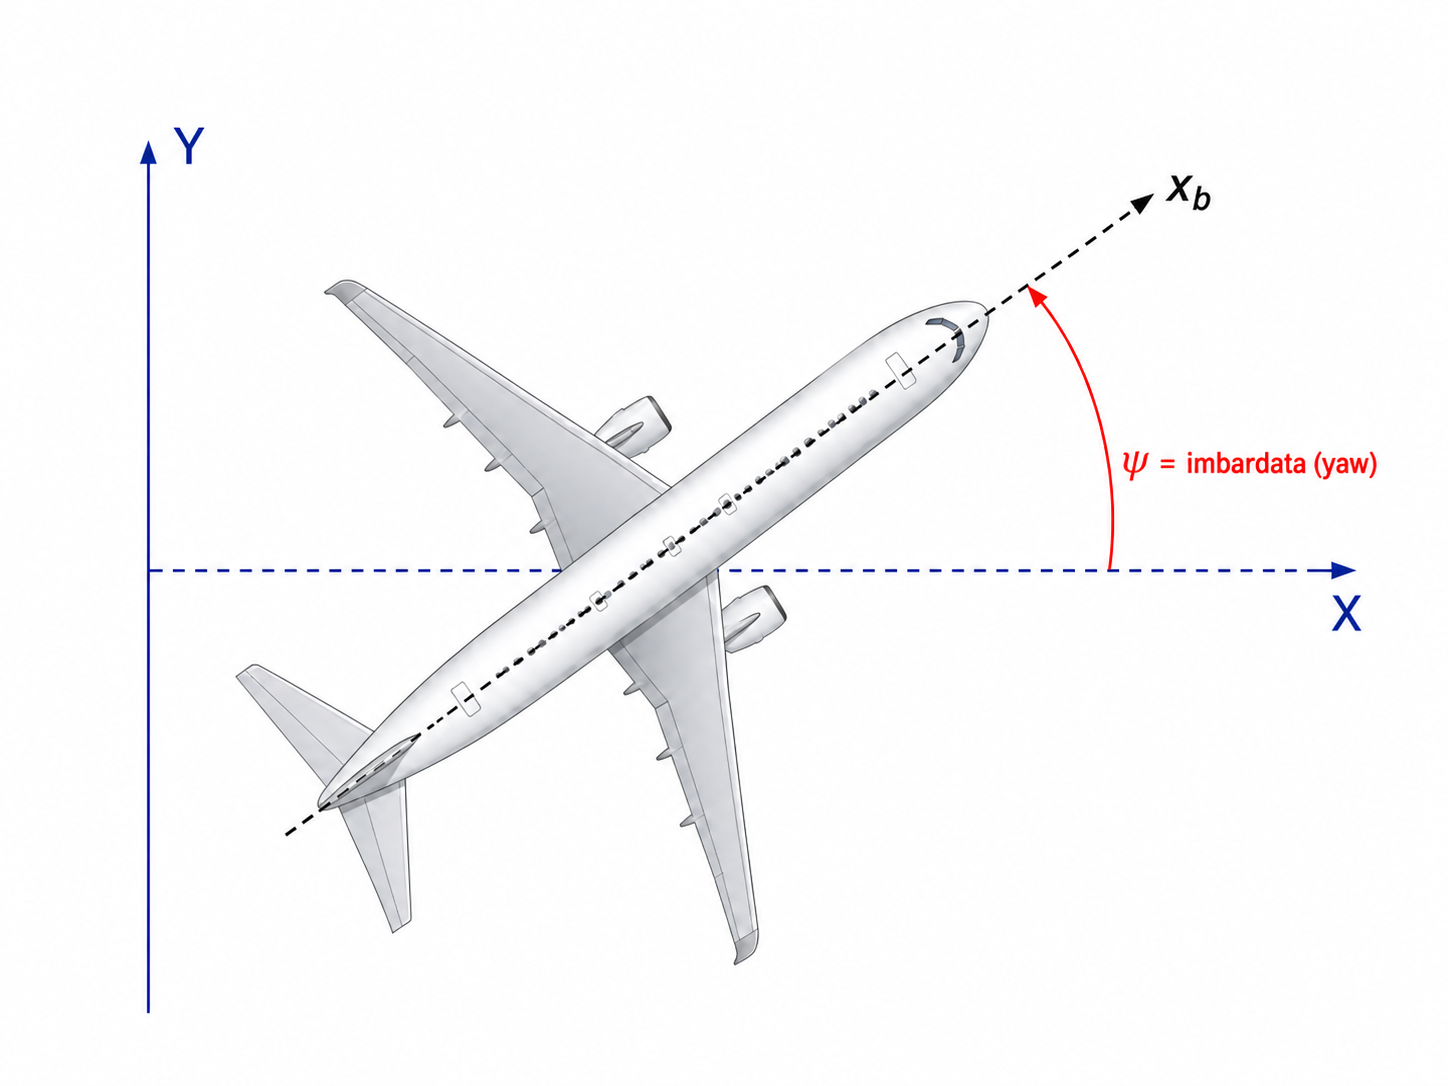
\includegraphics[width=\textwidth]{immagini/aereo1.PNG}
\end{minipage}
\hfill
\begin{minipage}{0.45\textwidth}
\centering
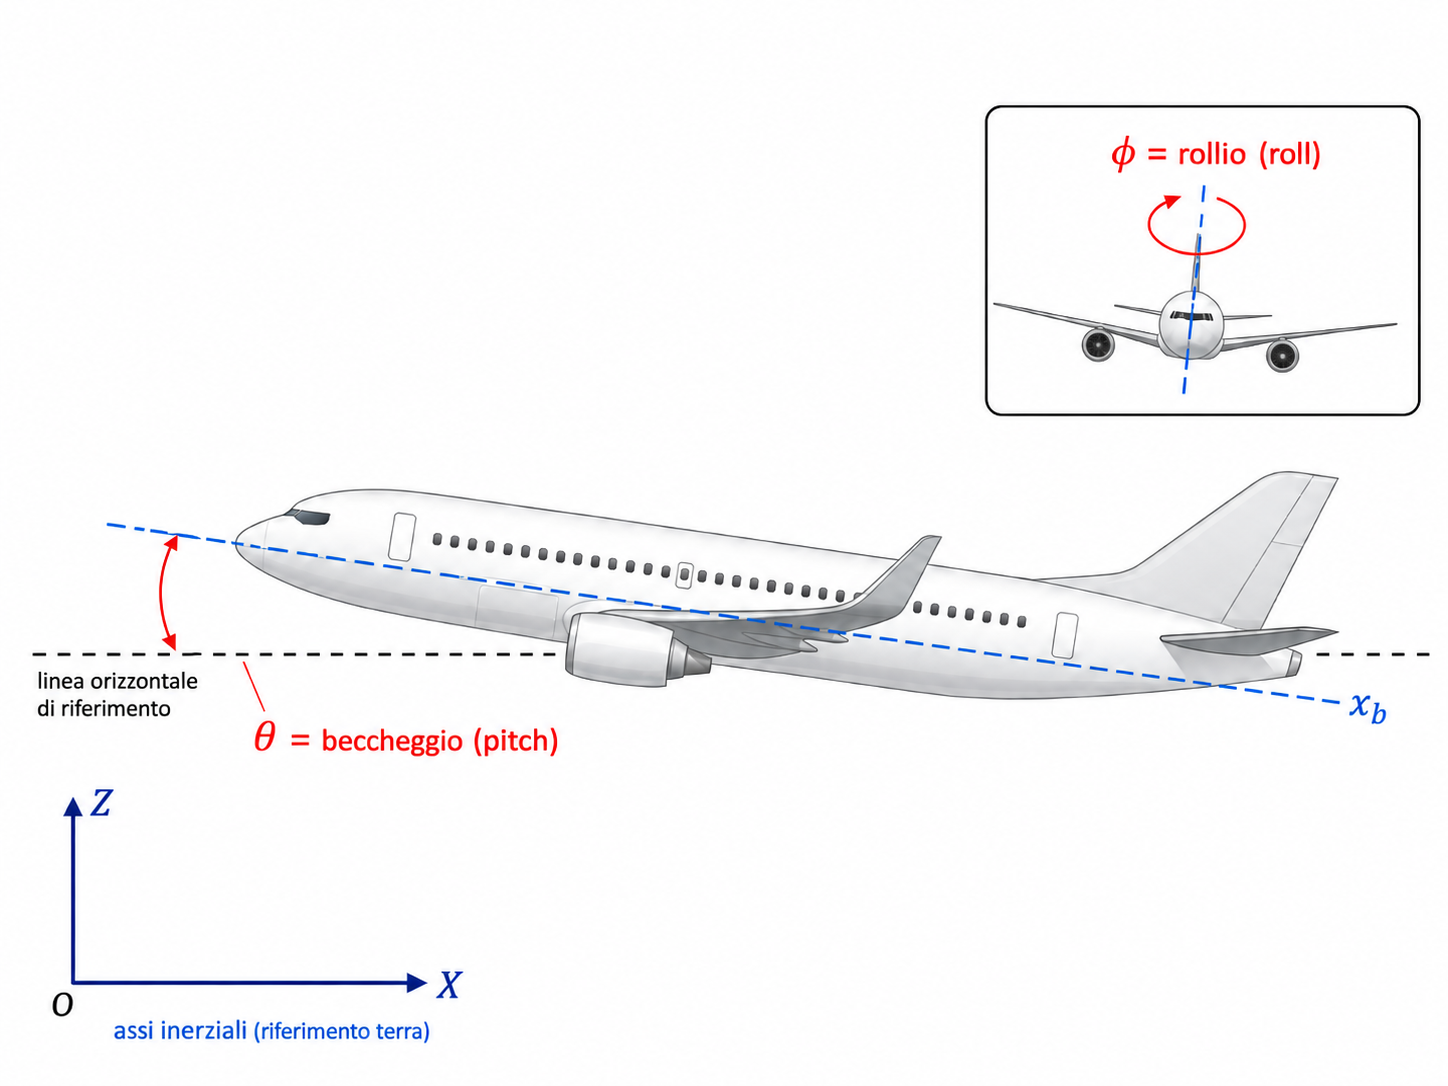
\includegraphics[width=\textwidth]{immagini/aereo2.PNG}
\end{minipage}
\end{center}

Presentiamo ora gli angoli di Eulero che, seppur più difficili da definire rispetto a quelli di Cardano, sono più utili ai nostri scopi.

\begin{definition}{}[Angoli di Eulero]
Consideriamo due riferimenti:
\[
\left\{O,\hat{\imath},\hat{\jmath},\hat{k}\right\}
\qquad \text{fisso}
\]
e
\[
\left\{O,\hat{\imath}',\hat{\jmath}',\hat{k}'\right\}
\qquad \text{mobile}.
\]

Definiamo gli angoli di Eulero come gli angoli associati alle  tre rotazioni antiorarie:

\begin{enumerate}[label=\roman*)]
\item Rotazione di un angolo $\varphi$ \textup{(precessione)} attorno all'asse $\hat{k}$ fino a quando $\hat{\imath}$ non interseca il piano definito da $\hat{\imath}'$, $\hat{\jmath}'$.

Chiamiamo $\hat{u}$ il versore dell'asse $\hat{\imath}$ trasportato dalla rotazione. $\hat{u}$ è detto versore della linea dei nodi.

\item Rotazione di un angolo $\theta$ \textup{(nutazione)} attorno alla linea dei nodi fino a che l'asse $\hat{k}$ va a sovrapporsi con $\hat{k}'$.

\item Rotazione di un angolo $\psi$ \textup{(rotazione propria)} attorno a $\hat{k}'$ fino a che $\hat{\imath}$, $\hat{\jmath}$ non si sovrappongono a $\hat{\imath}'$, $\hat{\jmath}'$.
\end{enumerate}
\end{definition}

\begin{center}
    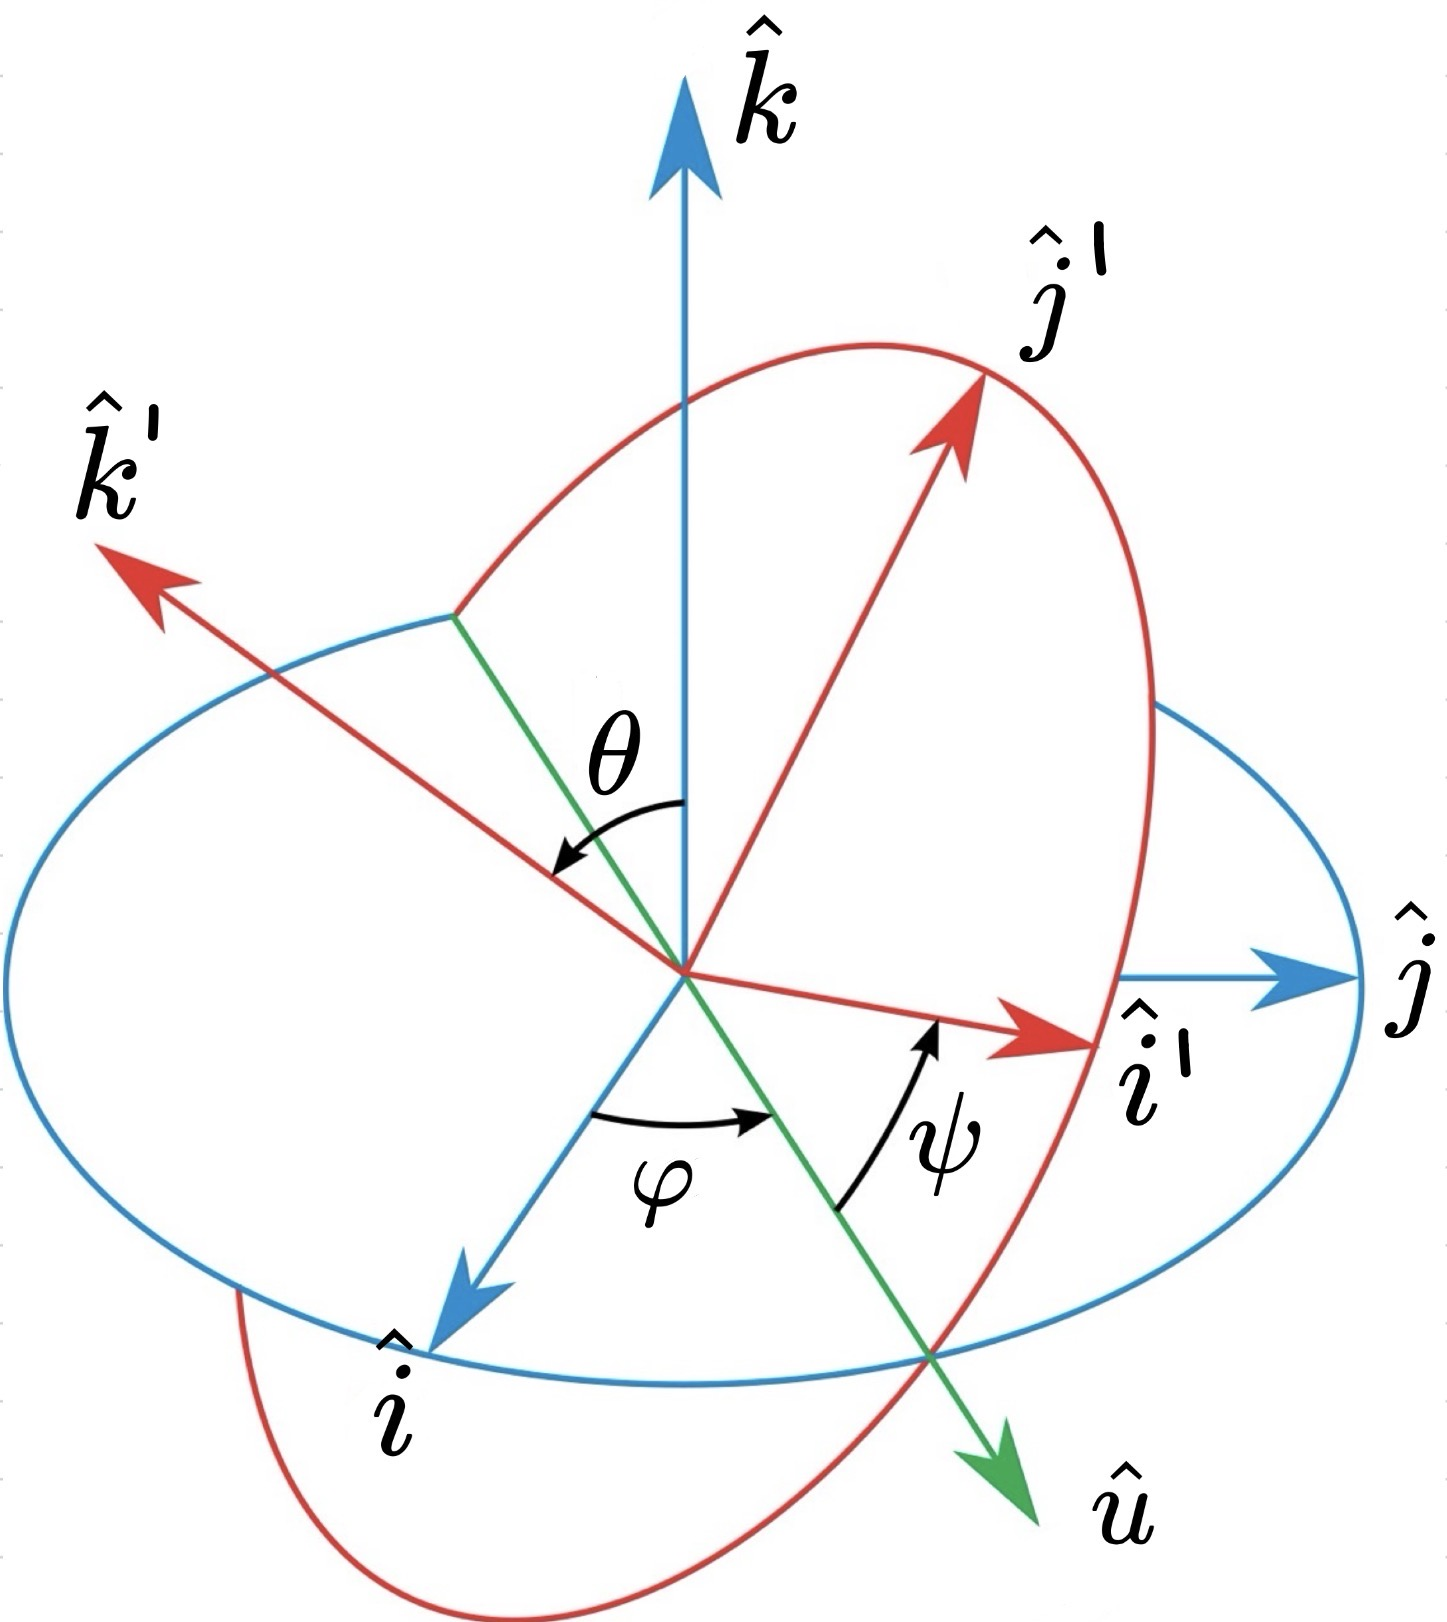
\includegraphics[scale=0.15]{immagini/angoli_eulero.jpg}
\end{center}

Per dare una trattazione matematica degli angoli di Eulero dobbiamo ricordare alcuni concetti di algebra lineare. Alcuni di questi sono già stati illustrati nel capitolo sulla formula fondamentale della cinematica e quindi li ricorderemo brevemente.

Consideriamo il gruppo delle rotazioni in $\mathbb{R}^n$
\[
R=\left\{R\in\mathbb{R}^{n,n}:\ R^TR=I_n,\ \det(R)=1\right\}.
\]

Questo è l'insieme di tutte le matrici ortogonali con determinante pari a $1$.

Iniziamo caratterizzando le rotazioni in $\mathbb{R}^2$. Consideriamo due basi ortonormali di $\mathbb{R}^2$
\[
\beta=\{\underline{e}_1,\underline{e}_2\},
\qquad
\beta'=\{\underline{e}_1',\underline{e}_2'\}
\]
tali che
\[
\underline{e}_1\cdot \underline{e}_1'=\underline{e}_2\cdot \underline{e}_2'=\cos\theta.
\]

\begin{center}
\begin{tikzpicture}[scale=1.2]
    % centro
    \coordinate (O) at (0,0);

    % cerchio
    \draw[thick] (O) circle (2);

    % assi / vettori della base beta
    \draw[->, very thick, green!60!black] (O) -- (2,0)
        node[below right] {$\underline{e}_1$};
    \draw[->, very thick, green!60!black] (O) -- (0,2)
        node[above] {$\underline{e}_2$};

    % vettori della base beta'
    \draw[->, very thick, red!80!black] (O) -- ({2*cos(45)},{2*sin(45)})
        node[above right] {$\underline{e}_1'$};
    \draw[->, very thick, red!80!black] (O) -- ({2*cos(135)},{2*sin(135)})
        node[above left] {$\underline{e}_2'$};

    % archi per theta
    \draw[thick] (0.8,0) arc[start angle=0,end angle=45,radius=0.8];
    \node at (0.95,0.35) {$\theta$};

    \draw[thick] ({0.7*cos(90)},{0.7*sin(90)}) arc[start angle=90,end angle=135,radius=0.7];
    \node at (-0.42,0.95) {$\theta$};
\end{tikzpicture}
\end{center}

Vogliamo trovare la rotazione $R \in \mathbb{R}^{2,2}$ tale che
\[
\underline{e}_1' = R\underline{e}_1,
\qquad
\underline{e}_2' = R\underline{e}_2.
\]

In particolare dovremmo trovare la matrice che rappresenta la rotazione rispetto a $\beta$ in partenza e in arrivo. Se però
\[
\underline{e}_1=(1,0)^T,
\qquad
\underline{e}_2=(0,1)^T,
\]
il conto è banale, infatti
\[
\underline{e}_1'=(\cos\theta,\sin\theta)^T,
\qquad
\underline{e}_2'=(-\sin\theta,\cos\theta)^T.
\]

Che implica che
\[
\begin{pmatrix}
r_{11} & r_{12}\\
r_{21} & r_{22}
\end{pmatrix}
\underline{e}_1
=
\begin{pmatrix}
r_{11} & r_{12}\\
r_{21} & r_{22}
\end{pmatrix}
\begin{pmatrix}
1\\
0
\end{pmatrix}
=
\begin{pmatrix}
r_{11}\\
r_{21}
\end{pmatrix}
=
\begin{pmatrix}
\cos\theta\\
\sin\theta
\end{pmatrix},
\]
\[
\begin{pmatrix}
r_{11} & r_{12}\\
r_{21} & r_{22}
\end{pmatrix}
\underline{e}_2
=
\begin{pmatrix}
r_{11} & r_{12}\\
r_{21} & r_{22}
\end{pmatrix}
\begin{pmatrix}
0\\
1
\end{pmatrix}
=
\begin{pmatrix}
r_{12}\\
r_{22}
\end{pmatrix}
=
\begin{pmatrix}
-\sin\theta\\
\cos\theta
\end{pmatrix}.
\]

Ovvero
\[
R=
\begin{pmatrix}
\cos\theta & -\sin\theta\\
\sin\theta & \cos\theta
\end{pmatrix}.
\]

È importante notare che $R$ è una rotazione attiva che mappa
\[
(\underline{e}_1,\underline{e}_2)
\quad \text{in} \quad
(\underline{e}_1',\underline{e}_2'),
\]
ovvero gira tutti i vettori del piano di un angolo $\theta$ in senso antiorario.

Per i nostri scopi però è più utile una matrice del cambio di base da $\beta$ a $\beta'$, ovvero una matrice che prende le componenti di un vettore $\underline{u}$ rispetto a $\beta$ e le mappa nelle componenti di $\underline{u}$ rispetto a $\beta'$.

Data l'importanza di $\beta$, le componenti di $\underline{u}$ rispetto a quest'ultima coincidono proprio con la descrizione che di solito diamo di $\underline{u}$, ovvero
\[
[\underline{u}]_{\beta}
=
\underline{u}
=
(u_1,u_2)^T.
\]

Ciò però non è più vero per quanto riguarda $\beta'$, ovvero
\[
\underline{u}
=
(u_1,u_2)^T
\neq
[\underline{u}]_{\beta'}
=
(u_1',u_2')^T.
\]

Ricordiamo infine che, in qualunque spazio vettoriale, la matrice $M_{\gamma}^{\gamma'}$ del cambio di base da $\gamma$ a $\gamma'$ è la matrice che rappresenta $\mathrm{id}_V$ rispetto a $\gamma$ in partenza e $\gamma'$ in arrivo.

Se lavoriamo con una base ortonormale, è particolarmente semplice ricavare le componenti di un vettore rispetto a quest'ultima. Infatti, se $\underline{u}\in \mathbb{R}^2$ e
\[
[\underline{u}]_{\beta}
=
(u_1,u_2)^T
=
\underline{u},
\qquad
[\underline{u}]_{\beta'}
=
(u_1',u_2')^T,
\]
è vero che
\[
(u_1',u_2')^T
=
\left(
\underline{u}\cdot \underline{e}_1',
\underline{u}\cdot \underline{e}_2'
\right)^T.
\]
Nel nostro caso
\[
(u_1',u_2')^T
=
\left(
\underline{u}\cdot \underline{e}_1',
\underline{u}\cdot \underline{e}_2'
\right)^T
=
\left(
(u_1\underline{e}_1+u_2\underline{e}_2)\cdot \underline{e}_1',
(u_1\underline{e}_1+u_2\underline{e}_2)\cdot \underline{e}_2'
\right)^T
\]
\[
=
\left(
u_1\,\underline{e}_1\cdot \underline{e}_1'
+
u_2\,\underline{e}_2\cdot \underline{e}_1',
u_1\,\underline{e}_1\cdot \underline{e}_2'
+
u_2\,\underline{e}_2\cdot \underline{e}_2'
\right)^T
\]
\[
=
\left(
u_1\cos\theta+u_2\sin\theta,
u_1\cos\left(\frac{\pi}{2}+\theta\right)+u_2\cos\theta
\right)^T
=
\left(
u_1\cos\theta+u_2\sin\theta,
-u_1\sin\theta+u_2\cos\theta
\right)^T
\]
\[
=
\begin{pmatrix}
\cos\theta & \sin\theta\\
-\sin\theta & \cos\theta
\end{pmatrix}
\begin{pmatrix}
u_1\\
u_2
\end{pmatrix}.
\]

Abbiamo quindi trovato che
\[
M_{\beta}^{\beta'}
=
R^T
=
R^{-1},
\]
ovvero è uguale alla rotazione attiva in senso orario di un angolo $\theta$.

Questo succede perché, quando operiamo un cambio di base, non stiamo effettivamente ruotando lo spazio, bensì stiamo cambiando il nostro punto di vista.

\begin{center}
\begin{tikzpicture}[scale=1]

% grafico sinistro
\begin{scope}[shift={(0,0)}]
\draw[thick] (0,0) circle (1.42);

\draw[->, very thick, green!60!black] (0,0) -- (1.45,0)
node[right] {$\underline{e}_1$};
\draw[->, very thick, green!60!black] (0,0) -- (0,1.45)
node[above] {$\underline{e}_2$};

\draw[->, very thick, red!80!black] (0,0) -- ({1.45*cos(40)},{1.45*sin(40)})
node[above right] {$\underline{e}_1'$};
\draw[->, very thick, red!80!black] (0,0) -- ({1.45*cos(130)},{1.45*sin(130)})
node[above left] {$\underline{e}_2'$};

\draw[->, thick] (0.65,0) arc[start angle=0,end angle=40,radius=0.65];
\node at (0.9,0.28) {$\theta$};

\draw[->, thick] (0,0.72) arc[start angle=90,end angle=130,radius=0.72];
\node at (-0.42,0.98) {$\theta$};
\end{scope}

% freccia centrale
\draw[->, thick] (2.8,0) -- (5.5,0);
\node[align=center] at (4.15,0.45) {cambio\\di base};

% grafico destro
\begin{scope}[shift={(8.2,0)}]
\draw[thick] (0,0) circle (1.42);

\draw[->, very thick, red!80!black] (0,0) -- (1.45,0)
node[right] {$\underline{e}_1'$};
\draw[->, very thick, red!80!black] (0,0) -- (0,1.45)
node[above] {$\underline{e}_2'$};

\draw[->, very thick, green!60!black] (0,0) -- ({1.45*cos(-40)},{1.45*sin(-40)})
node[below right] {$\underline{e}_1$};
\draw[->, very thick, green!60!black] (0,0) -- ({1.45*cos(50)},{1.45*sin(50)})
node[above right] {$\underline{e}_2$};

\draw[->, thick] (0.7,0) arc[start angle=0,end angle=-40,radius=0.7];
\node at (0.95,-0.3) {$\theta$};

\draw[->, thick] (0,0.78) arc[start angle=90,end angle=50,radius=0.78];
\node at (0.45,1.02) {$\theta$};
\end{scope}

\end{tikzpicture}
\end{center}

I vettori ci appaiono così ruotati di un angolo $\theta$ in senso orario rispetto a come li vedevamo prima del cambio di base.

Un'altra classe di rotazioni che ci sono utili sono le rotazioni in $\mathbb{R}^3$ rispetto ad un asse fisso.

Partiremo con la descrizione della rotazione attiva attorno all'asse $z$, per poi descrivere il suo cambio di base associato. Daremo infine solo l'espressione delle rotazioni attive attorno all'asse $x$ e $y$ e dei loro cambi di base associati, in quanto questi si ricavano in modo analogo.

Sia
\[
\beta=\{\underline{e}_1,\underline{e}_2,\underline{e}_3\}
\]
la base canonica di $\mathbb{R}^3$ e sia
\[
\beta'=\{\underline{e}_1',\underline{e}_2',\underline{e}_3'\}
\]
la base ortonormale tale che
\[
\underline{e}_1\cdot \underline{e}_1'
=
\underline{e}_2\cdot \underline{e}_2'
=
\cos\theta,
\qquad
\underline{e}_3=\underline{e}_3'.
\]
\begin{center}
    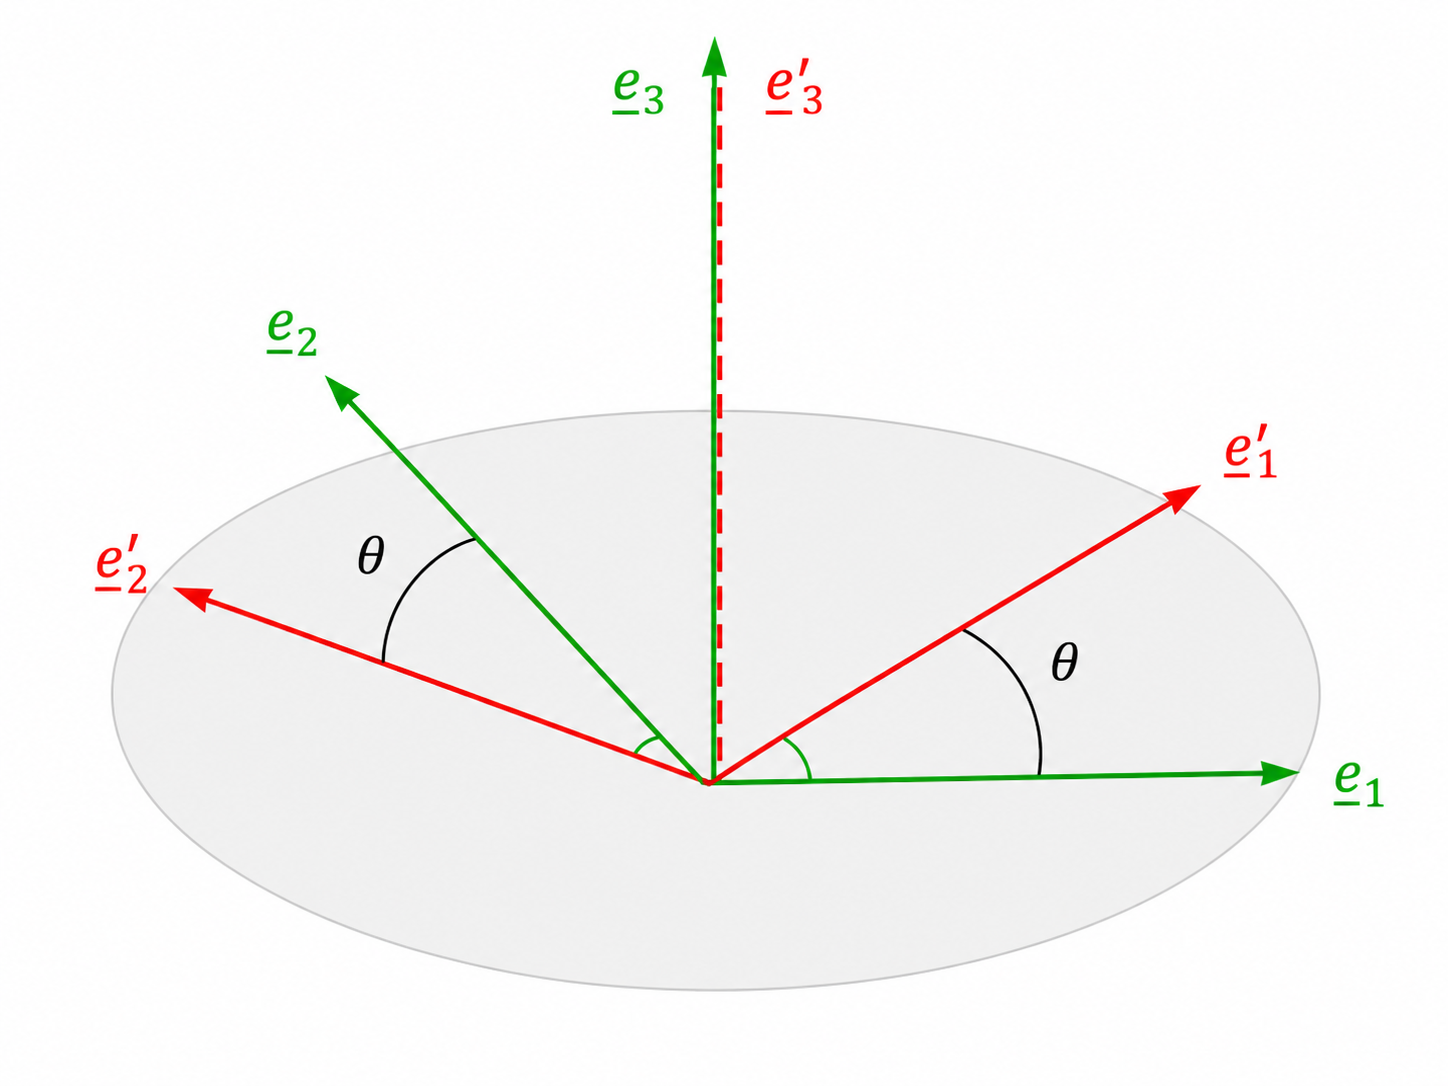
\includegraphics[scale=0.2]{immagini/basi_ortonormali.PNG}
\end{center}

Vogliamo trovare $R_z \in \mathbb{R}^{3,3}$ ortogonale tale che
\[
\underline{e}_1' = R_z \underline{e}_1,
\qquad
\underline{e}_2' = R_z \underline{e}_2,
\qquad
\underline{e}_3' = \underline{e}_3 = R_z\underline{e}_3.
\]

Procediamo come fatto nel caso bidimensionale:
\[
\underline{e}_1' = (\cos\theta,\sin\theta,0)^T,
\qquad
\underline{e}_2' = (-\sin\theta,\cos\theta,0)^T,
\qquad
\underline{e}_3' = (0,0,1)^T.
\]

\[
\begin{pmatrix}
r_{11} & r_{12} & r_{13}\\
r_{21} & r_{22} & r_{23}\\
r_{31} & r_{32} & r_{33}
\end{pmatrix}
\underline{e}_1
=
\begin{pmatrix}
r_{11} & r_{12} & r_{13}\\
r_{21} & r_{22} & r_{23}\\
r_{31} & r_{32} & r_{33}
\end{pmatrix}
\begin{pmatrix}
1\\
0\\
0
\end{pmatrix}
=
\begin{pmatrix}
r_{11}\\
r_{21}\\
r_{31}
\end{pmatrix}
=
\begin{pmatrix}
\cos\theta\\
\sin\theta\\
0
\end{pmatrix}
=
\underline{e}_1'.
\]

\[
\begin{pmatrix}
r_{11} & r_{12} & r_{13}\\
r_{21} & r_{22} & r_{23}\\
r_{31} & r_{32} & r_{33}
\end{pmatrix}
\underline{e}_2
=
\begin{pmatrix}
r_{11} & r_{12} & r_{13}\\
r_{21} & r_{22} & r_{23}\\
r_{31} & r_{32} & r_{33}
\end{pmatrix}
\begin{pmatrix}
0\\
1\\
0
\end{pmatrix}
=
\begin{pmatrix}
r_{12}\\
r_{22}\\
r_{32}
\end{pmatrix}
=
\begin{pmatrix}
-\sin\theta\\
\cos\theta\\
0
\end{pmatrix}
=
\underline{e}_2'.
\]

\[
\begin{pmatrix}
r_{11} & r_{12} & r_{13}\\
r_{21} & r_{22} & r_{23}\\
r_{31} & r_{32} & r_{33}
\end{pmatrix}
\underline{e}_3
=
\begin{pmatrix}
r_{11} & r_{12} & r_{13}\\
r_{21} & r_{22} & r_{23}\\
r_{31} & r_{32} & r_{33}
\end{pmatrix}
\begin{pmatrix}
0\\
0\\
1
\end{pmatrix}
=
\begin{pmatrix}
r_{13}\\
r_{23}\\
r_{33}
\end{pmatrix}
=
\begin{pmatrix}
0\\
0\\
1
\end{pmatrix}
=
\underline{e}_3'.
\]

Ovvero
\[
R_z
=
\begin{pmatrix}
\cos\theta & -\sin\theta & 0\\
\sin\theta & \cos\theta & 0\\
0 & 0 & 1
\end{pmatrix}.
\]

Anche in questo caso questa è la rotazione attiva. Siamo però più interessati al cambio di base da $\beta$ a $\beta'$, ovvero $M_{\beta}^{\beta'}$ tale che
\[
[\underline{u}]_{\beta'}
=
M_{\beta}^{\beta'}[\underline{u}]_{\beta}
\qquad
\forall \underline{u}\in\mathbb{R}^3.
\]

Come nel caso bidimensionale ci facciamo aiutare dal fatto che $\beta'$ è una base ortonormale e quindi, dato
\[
\underline{u}
=
[\underline{u}]_{\beta}
=
(u_1,u_2,u_3)^T
\in \mathbb{R}^3,
\]
è vero che
\[
[\underline{u}]_{\beta'}
=
\left(
\underline{u}\cdot \underline{e}_1',
\underline{u}\cdot \underline{e}_2',
\underline{u}\cdot \underline{e}_3'
\right)^T
\]
\[
=
\begin{pmatrix}
\left[u_1\underline{e}_1+u_2\underline{e}_2+u_3\underline{e}_3\right]\cdot \underline{e}_1'
\\[4pt]
\left[u_1\underline{e}_1+u_2\underline{e}_2+u_3\underline{e}_3\right]\cdot \underline{e}_2'
\\[4pt]
\left[u_1\underline{e}_1+u_2\underline{e}_2+u_3\underline{e}_3\right]\cdot \underline{e}_3'
\end{pmatrix}
\]
\[
=
\begin{pmatrix}
u_1\cos\theta+u_2\sin\theta
\\
-u_1\sin\theta+u_2\cos\theta
\\
u_3
\end{pmatrix}
=
\begin{pmatrix}
\cos\theta & \sin\theta & 0
\\
-\sin\theta & \cos\theta & 0
\\
0 & 0 & 1
\end{pmatrix}
\begin{pmatrix}
u_1\\
u_2\\
u_3
\end{pmatrix}.
\]

Anche qui abbiamo ottenuto che
\[
M_{\beta}^{\beta'}
=
R_z^T
=
R_z^{-1}.
\]

Il motivo è lo stesso del caso bidimensionale: non stiamo ruotando lo spazio, ma stiamo cambiando il nostro punto di vista.

Le matrici di rotazione rispetto all'asse $x$ e all'asse $y$ sono
\[
R_x
=
\begin{pmatrix}
1 & 0 & 0
\\
0 & \cos\theta & -\sin\theta
\\
0 & \sin\theta & \cos\theta
\end{pmatrix},
\qquad
R_y
=
\begin{pmatrix}
\cos\theta & 0 & \sin\theta
\\
0 & 1 & 0
\\
-\sin\theta & 0 & \cos\theta
\end{pmatrix}.
\]

I corrispondenti cambi di base sono
\[
R_x^T,
\qquad
R_y^T.
\]

Siamo finalmente pronti a dare una descrizione matematica agli angoli di Eulero. In particolare siano
\[
\gamma=\{\hat{\imath},\hat{\jmath},\hat{k}\},
\qquad
\gamma'=\{\hat{\imath}',\hat{\jmath}',\hat{k}'\},
\]
troviamo $M_{\gamma}^{\gamma'}$.

Le rotazioni che abbiamo descritto nella definizione degli angoli di Eulero sono le rotazioni attive date dalle matrici
\[
\text{(i)} \qquad
C^T=
\begin{pmatrix}
\cos\varphi & -\sin\varphi & 0\\
\sin\varphi & \cos\varphi & 0\\
0 & 0 & 1
\end{pmatrix},
\]
\[
\text{(ii)} \qquad
B^T=
\begin{pmatrix}
1 & 0 & 0\\
0 & \cos\theta & -\sin\theta\\
0 & \sin\theta & \cos\theta
\end{pmatrix},
\]
\[
\text{(iii)} \qquad
A^T=
\begin{pmatrix}
\cos\psi & -\sin\psi & 0\\
\sin\psi & \cos\psi & 0\\
0 & 0 & 1
\end{pmatrix}.
\]

Attenzione però al fatto che la nutazione e la rotazione propria non sono attorno agli assi $\hat{k}$ e $\hat{\imath}$ nel riferimento fisso, ma rispetto ad assi intermedi.

Scrivere che la rotazione attiva è data da
\[
A^TB^TC^T
\]
sarebbe quindi sbagliato. La giusta matrice è
\[
C^TB^TA^T.
\]
Vediamo perché.

\begin{enumerate}[label=\roman*)]
\item Il vettore $\hat{\imath}$ viene mandato in $\hat{u}$ attraverso $C^T$, ovvero
\[
\hat{u}=C^T\hat{\imath}.
\]

\item Ora dobbiamo applicare la rotazione $B^T$ attorno all'asse dei nodi. Per farlo facciamo un passo indietro: applichiamo la rotazione a $\hat{\imath}$, ovvero $B^T\hat{\imath}$, e poi riportiamo tutto attorno a $\hat{u}$, ovvero
\[
C^TB^T\hat{\imath}.
\]
In questo modo $\hat{\imath}$ viene ancora mappato in $\hat{u}$, infatti
\[
C^TB^T\hat{\imath}
=
C^T\hat{\imath}
=
\hat{u}.
\]

\item Infine vogliamo effettuare la rotazione attorno a $\hat{k}'$. Allo stesso modo torniamo indietro, applichiamo $A^T$ a $\hat{k}$, ovvero $A^T\hat{k}$, poi ruotiamo di nuovo con $C^TB^T$. Come verifica controlliamo dove viene mandato $\hat{k}$:
\[
C^TB^TA^T\hat{k}
=
C^TB^T\hat{k}
=
\hat{k}'.
\]
\end{enumerate}

Il cambio di base associato è quindi
\[
M_{\gamma}^{\gamma'}
=
(C^TB^TA^T)^T
=
ABC,
\]
con
\[
A=
\begin{pmatrix}
\cos\psi & \sin\psi & 0\\
-\sin\psi & \cos\psi & 0\\
0 & 0 & 1
\end{pmatrix},
\]
\[
B=
\begin{pmatrix}
1 & 0 & 0\\
0 & \cos\theta & \sin\theta\\
0 & -\sin\theta & \cos\theta
\end{pmatrix},
\]
\[
C=
\begin{pmatrix}
\cos\varphi & \sin\varphi & 0\\
-\sin\varphi & \cos\varphi & 0\\
0 & 0 & 1
\end{pmatrix}.
\]
\vspace{30pt}
\section{Il moto della trottola}

La trottola è un modello per un corpo rigido dotato di un asse di simmetria soggetto alla forza peso e con un punto fisso.

\begin{center}
    \begin{tikzpicture}[scale=1.15,>=Latex]

\coordinate (O) at (0,0);

% angoli dei vari assi
\def\angi{-145}
\def\angu{-112}
\def\angip{-55}
\def\angjp{42}
\def\angkp{125}

% assi fissi
\coordinate (I) at ($(O)+(\angi:4.2)$);
\coordinate (J) at ($(O)+(0:5.4)$);
\coordinate (K) at ($(O)+(90:4.8)$);

% assi principali d'inerzia
\coordinate (Ip) at ($(O)+(\angip:4.2)$);
\coordinate (Jp) at ($(O)+(\angjp:4.7)$);
\coordinate (Kp) at ($(O)+(\angkp:4.8)$);

% linea dei nodi
\coordinate (U) at ($(O)+(\angu:3.1)$);

% centro di massa su k'
\coordinate (G) at ($(O)+(\angkp:2.05)$);

%------------------------------------------------
% trottola stilizzata, allineata con k'
% disegnata inizialmente lungo l'asse y e poi ruotata
\begin{scope}[shift={(O)},rotate=35]

  % corpo principale
  \filldraw[fill=white,draw=black,thick]
    (0,0)
    .. controls (-0.10,0.26) and (-0.58,0.88) .. (-0.98,1.60)
    .. controls (-1.25,2.15) and (-1.22,2.88) .. (-0.58,3.35)
    .. controls (-0.36,3.52) and (-0.22,3.70) .. (-0.18,3.90)
    -- (0.18,3.90)
    .. controls (0.22,3.70) and (0.36,3.52) .. (0.58,3.35)
    .. controls (1.22,2.88) and (1.25,2.15) .. (0.98,1.60)
    .. controls (0.58,0.88) and (0.10,0.26) .. (0,0)
    -- cycle;

  % collarino vicino alla punta
  \draw[thick]
    (-0.16,0.52) .. controls (-0.08,0.60) and (0.08,0.60) .. (0.16,0.52);
  \draw[thick]
    (-0.13,0.44) .. controls (-0.05,0.50) and (0.05,0.50) .. (0.13,0.44);

  % anelli decorativi
  \draw[thick]
    (-0.76,1.78) .. controls (-0.32,1.98) and (0.32,1.98) .. (0.76,1.78);
  \draw[thick]
    (-0.94,2.42) .. controls (-0.40,2.66) and (0.40,2.66) .. (0.94,2.42);
  \draw[thick]
    (-0.74,3.02) .. controls (-0.28,3.22) and (0.28,3.22) .. (0.74,3.02);

  % pomello superiore
  \draw[thick]
    (-0.18,3.90) .. controls (-0.22,4.05) and (-0.30,4.15) .. (-0.18,4.25);
  \draw[thick]
    (0.18,3.90) .. controls (0.22,4.05) and (0.30,4.15) .. (0.18,4.25);
  \draw[thick] (0,4.25) ellipse[x radius=0.18,y radius=0.06];

\end{scope}
%------------------------------------------------
% assi fissi
\draw[->,very thick] (O) -- (J) node[right] {$\hat j$};
\draw[->,very thick] (O) -- (K) node[above] {$\hat k$};
\draw[->,very thick] (O) -- (I) node[below left] {$\hat i$};

% assi principali d'inerzia
\draw[->,red!80!black,dashed,thick] (O) -- (Kp) node[above left] {$\hat k'$};
\draw[->,red!80!black,dashed,thick] (O) -- (Jp) node[above right] {$\hat j'$};
\draw[->,red!80!black,dashed,thick] (O) -- (Ip) node[below right] {$\hat i'$};

% linea dei nodi
\draw[->,violet,very thick] (O) -- (U) node[below] {$\underline{u}$};



%------------------------------------------------
% centro di massa
\fill[green!60!black] (G) circle (2.4pt);
\node[above right=1pt,green!60!black] at (G) {$G$};

% forza peso
\draw[->,green!60!black,thick] (G) -- ++(0,-1.9) node[below left] {$m\underline{g}$};

% graffa per il segmento d = OG
\draw[
  green!60!black,
  thick,
  decorate,
  decoration={brace,amplitude=6pt}
]
  ($(O)+(215:0.30)$) -- ($(G)+(215:0.30)$)
  node[midway,left=8pt] {$d$};

%------------------------------------------------
% angoli di Eulero
\draw[orange!85!black,thick]
  ($(O)+(\angi:1.02)$)
  arc[start angle=\angi,end angle=\angu,radius=1.02];
\node[orange!85!black] at ($(O)+(-129:1.28)$) {$\varphi$};

\draw[orange!85!black,thick]
  ($(O)+(90:1.14)$)
  arc[start angle=90,end angle=\angkp,radius=1.14];
\node[orange!85!black] at ($(O)+(108:1.45)$) {$\theta$};

\draw[orange!85!black,thick]
  ($(O)+(\angu:0.84)$)
  arc[start angle=\angu,end angle=\angip,radius=0.84];
\node[orange!85!black] at ($(O)+(-84:1.02)$) {$\psi$};

% origine
\fill (O) circle (2pt);

\end{tikzpicture}
\end{center}

Impostiamo due sistemi di riferimento:
\[
\beta=\{\hat{i},\hat{j},\hat{k}\}
\quad \text{fisso}
\qquad \text{e} \qquad
\beta'=\{\hat{i}',\hat{j}',\hat{k}'\}
\quad \text{solidale}.
\]

L'asse \(\hat{k}'\) è anche asse di simmetria.

Scriviamo le equazioni del moto. Il sistema ha \(3\) gradi di libertà.
Scegliamo come coordinate libere gli angoli di Eulero.

Il sistema ha energia potenziale
\[
V = mgd\cos\theta.
\]

Se impostiamo \(\hat{i}',\hat{j}',\hat{k}'\) lungo gli assi principali d'inerzia, il tensore d'inerzia risulta diagonale:
\[
I_C =
\begin{pmatrix}
I & 0 & 0\\
0 & I & 0\\
0 & 0 & I_0
\end{pmatrix}.
\]

\[
T =
\frac{1}{2}
[\underline{\omega}]_{\beta'} \cdot I_C [\underline{\omega}]_{\beta'}
\]
dove \([\underline{\omega}]_{\beta'}\) è il vettore delle componenti di
\(\underline{\omega}\) rispetto a \(\beta'\).

Scegliamo, per ragioni fisiche, di rappresentare
\[
\underline{\omega}
=
\dot{\varphi}\hat{k}
+
\dot{\theta}\,\underline{u}
+
\dot{\psi}\hat{k}'.
\]

Dobbiamo scrivere \(\underline{\omega}\) lungo
\[
\{\hat{i}',\hat{j}',\hat{k}'\}.
\]

Usiamo i \(3\) cambi di base ABC definiti nel paragrafo precedente:
\[
\begin{pmatrix}
\cos\psi & \sin\psi & 0\\
-\sin\psi & \cos\psi & 0\\
0 & 0 & 1
\end{pmatrix}
\begin{pmatrix}
\dot{\theta}\\
0\\
0
\end{pmatrix}
=
\dot{\theta}
\begin{pmatrix}
\cos\psi\\
-\sin\psi\\
0
\end{pmatrix}.
\]

Quindi
\[
\dot{\theta}\,\underline{u}
=
\dot{\theta}\cos\psi\,\hat{i}'
-
\dot{\theta}\sin\psi\,\hat{j}'.
\]
\[
\begin{pmatrix}
\cos\psi & \sin\psi & 0\\
-\sin\psi & \cos\psi & 0\\
0 & 0 & 1
\end{pmatrix}
\begin{pmatrix}
1 & 0 & 0\\
0 & \cos\theta & \sin\theta\\
0 & -\sin\theta & \cos\theta
\end{pmatrix}
\begin{pmatrix}
0\\
0\\
\dot{\varphi}
\end{pmatrix}
=
\begin{pmatrix}
\cos\psi & \sin\psi & 0\\
-\sin\psi & \cos\psi & 0\\
0 & 0 & 1
\end{pmatrix}
\begin{pmatrix}
0\\
\sin\theta\,\dot{\varphi}\\
\cos\theta\,\dot{\varphi}
\end{pmatrix}
=
\]

\[
=
\begin{pmatrix}
\sin\psi\sin\theta\,\dot{\varphi}\\
\cos\psi\sin\theta\,\dot{\varphi}\\
\cos\theta\,\dot{\varphi}
\end{pmatrix}^{T}
\]

\[
\Rightarrow
\dot{\varphi}\hat{k}
=
\sin\psi\sin\theta\,\dot{\varphi}\,\hat{i}'
+
\cos\psi\sin\theta\,\dot{\varphi}\,\hat{j}'
+
\cos\theta\,\dot{\varphi}\,\hat{k}'.
\]

\[
\Rightarrow
\underline{\omega}
=
\left(
\dot{\theta}\cos\psi
+
\sin\psi\sin\theta\,\dot{\varphi}
\right)\hat{i}'
+
\left(
-\dot{\theta}\sin\psi
+
\cos\psi\sin\theta\,\dot{\varphi}
\right)\hat{j}'
+
\left(
\dot{\psi}
+
\cos\theta\,\dot{\varphi}
\right)\hat{k}'.
\]

Possiamo quindi scrivere l'energia cinetica.

\[
\begin{aligned}
2T
&=
[\underline{\omega}]_{\beta'}\cdot I_C[\underline{\omega}]_{\beta'}\\
&=
I\left(
\dot{\theta}\cos\psi
+
\sin\psi\sin\theta\,\dot{\varphi}
\right)^2
+
I\left(
-\dot{\theta}\sin\psi
+
\dot{\varphi}\cos\psi\sin\theta
\right)^2
+
I_0
\left(
\dot{\psi}
+
\dot{\varphi}\cos\theta
\right)^2.
\end{aligned}
\]

\[
\begin{aligned}
&=
I\left(
\dot{\theta}^2\cos^2\psi
+
\sin^2\psi\sin^2\theta\,\dot{\varphi}^2
+
2\dot{\theta}\cos\psi\sin\psi\sin\theta\,\dot{\varphi}
\right)\\
&\quad+
I\left(
\dot{\theta}^2\sin^2\psi
+
\dot{\varphi}^2\cos^2\psi\sin^2\theta
-
2\dot{\theta}\sin\psi\cos\psi\sin\theta\,\dot{\varphi}
\right)\\
&\quad+
I_0
\left(
\dot{\psi}
+
\dot{\varphi}\cos\theta
\right)^2\\
&=
I\left(
\dot{\theta}^2\cos^2\psi
+
\sin^2\psi\sin^2\theta\,\dot{\varphi}^2
+
\dot{\theta}^2\sin^2\psi
+
\dot{\varphi}^2\cos^2\psi\sin^2\theta
\right)\\
&\quad+
I_0
\left(
\dot{\psi}
+
\dot{\varphi}\cos\theta
\right)^2\\
&=
I\dot{\theta}^2
+
I\sin^2\theta\,\dot{\varphi}^2
+
I_0
\left(
\dot{\psi}
+
\dot{\varphi}\cos\theta
\right)^2.
\end{aligned}
\]

\[
\mathcal{L}
=
T-V
=
\frac{I}{2}
\left(
\dot{\theta}^2
+
\sin^2\theta\,\dot{\varphi}^2
\right)
+
\frac{I_0}{2}
\left(
\dot{\psi}
+
\dot{\varphi}\cos\theta
\right)^2
-
mgd\cos\theta.
\]

Notiamo che \(\mathcal{L}\) non dipende da \(\varphi\) e da \(\psi\), allora
\[
\frac{\partial \mathcal{L}}{\partial \dot{\varphi}},
\qquad
\frac{\partial \mathcal{L}}{\partial \dot{\psi}}
\]
sono costanti nel tempo.

\[
\frac{\partial \mathcal{L}}{\partial \dot{\varphi}}
=
I\sin^2\theta\,\dot{\varphi}
+
I_0
\left(
\dot{\psi}
+
\dot{\varphi}\cos\theta
\right)\cos\theta
=
\left.
\frac{\partial \mathcal{L}}{\partial \dot{\varphi}}
\right|_{t=0}
=
Ib,
\qquad b\in\mathbb{R}.
\]

\[
\frac{\partial \mathcal{L}}{\partial \dot{\psi}}
=
I_0
\left(
\dot{\psi}
+
\dot{\varphi}\cos\theta
\right)
=
\left.
\frac{\partial \mathcal{L}}{\partial \dot{\psi}}
\right|_{t=0}
=
Ia,
\qquad a\in\mathbb{R}.
\]

Vogliamo ottenere \(2\) equazioni disaccoppiate. Sostituisco \(Ia\) nella prima

\[
I\sin^2\theta\,\dot{\varphi}
+
Ia\cos\theta
=
Ib
\Rightarrow
\sin^2\theta\,\dot{\varphi}
+
a\cos\theta
=
b
\Rightarrow
\dot{\varphi}
=
\frac{b-a\cos\theta}{\sin^2\theta}.
\]

La trottola è sottoposta solo a forze conservative e quindi l'energia meccanica si conserva

\[
\frac{I}{2}
\left(
\dot{\theta}^2
+
\sin^2\theta\,\dot{\varphi}^2
\right)
+
\frac{I_0}{2}
\left(
\dot{\psi}
+
\dot{\varphi}\cos\theta
\right)^2
+
mgd\cos\theta
=
E.
\]
Da
\[
\frac{\partial \mathcal{L}}{\partial \dot{\psi}} = Ia
\]
otteniamo
\[
\left(\dot{\psi}+\dot{\varphi}\cos\theta\right)^2
=
\frac{I^2a^2}{I_0^2}
\]
e quindi
\[
\frac{I}{2}
\left(
\dot{\theta}^2+\sin^2\theta\,\dot{\varphi}^2
\right)
+
\frac{I^2a^2}{2I_0}
+
mgd\cos\theta
=
E.
\]

Dal momento che
\[
\dot{\varphi}
=
\frac{b-a\cos\theta}{\sin^2\theta},
\]
si ha
\[
\frac{I}{2}
\left(
\dot{\theta}^2
+
\frac{\left(b-a\cos\theta\right)^2}{\sin^2\theta}
\right)
+
\frac{I^2a^2}{2I_0}
+
mgd\cos\theta
=
E.
\]

\[
\Rightarrow
\frac{2E}{I}
=
\frac{2}{I}\cdot\frac{I^2a^2}{2I_0}
+
\dot{\theta}^2
+
\frac{\left(b-a\cos\theta\right)^2}{\sin^2\theta}
+
\frac{2}{I}mgd\cos\theta.
\]

\[
\Rightarrow
\dot{\theta}^2
+
\frac{\left(b-a\cos\theta\right)^2}{\sin^2\theta}
+
\frac{2}{I}mgd\cos\theta
=
\frac{2E}{I}
-
\frac{Ia^2}{I_0}.
\]

Ponendo
\[
\alpha
=
\frac{2E}{I}
-
\frac{Ia^2}{I_0}
\qquad
\text{e}
\qquad
\beta
=
\frac{2}{I}mgd,
\]
ottengo
\[
\dot{\theta}^2
+
\frac{\left(b-a\cos\theta\right)^2}{\sin^2\theta}
+
\beta\cos\theta
=
\alpha
\Rightarrow
\dot{\theta}^2
=
\alpha
-
\frac{\left(b-a\cos\theta\right)^2}{\sin^2\theta}
-
\beta\cos\theta.
\]

Abbiamo ottenuto un'equazione differenziale del primo ordine disaccoppiata.

Proviamo un cambio di variabile

\[
\Rightarrow
\dot{\theta}^2
=
\alpha
-
\frac{\left(b-a\cos\theta\right)^2}{1-\cos^2\theta}
-
\beta\cos\theta.
\]

\[
\Rightarrow
\left(1-\cos^2\theta\right)\dot{\theta}^2
=
\alpha\left(1-\cos^2\theta\right)
-
\left(b-a\cos\theta\right)^2
-
\beta\left(1-\cos^2\theta\right)\cos\theta.
\]

Pongo
\[
u=\cos\theta,
\qquad
\dot{u}=-\sin\theta\,\dot{\theta},
\qquad
\dot{u}^2
=
\sin^2\theta\,\dot{\theta}^2
=
\left(1-\cos^2\theta\right)\dot{\theta}^2.
\]

\[
\dot{u}^2
=
\alpha\left(1-u^2\right)
-
\left(b-au\right)^2
-
\beta\left(1-u^2\right)u.
\]

\[
\Rightarrow
\dot{u}^2
=
(\alpha-\beta u)(1-u^2)-(b-au)^2
\qquad
\alpha,\beta,a,b \text{ noti}
\]

Studiamo segni e zeri del polinomio \(p(u)\) a secondo membro. Iniziamo con i limiti agli estremi del dominio

\[
\lim_{u\to +\infty} (\alpha-\beta u)(1-u^2)-(b-au)^2
=
\lim_{u\to +\infty} \beta u^3
=
+\infty
\]

\[
\lim_{u\to -\infty} (\alpha-\beta u)(1-u^2)-(b-au)^2
=
\lim_{u\to -\infty} \beta u^3
=
-\infty
\]

Ricordando che
\[
\beta=\frac{2}{I}mgd>0
\]

Notiamo ora che \(p(1)=p(-1)=-(b-a)^2<0\). L'equazione differenziale di incognita \(u(t)\) è una EDO del primo ordine per la quale siamo certi esista una soluzione locale (teorema di esistenza ed unicità). La soluzione può esistere solo se \(p(u)\) ammette valori positivi nell'intervallo in \(S\subseteq[-1,1]\). Infatti essendo \(\dot{u}^2=p(u)\) allora \(p(u)\) deve essere non negativo ed inoltre \(u=\cos\theta \Rightarrow u\in[-1,1]\). Possiamo anche escludere l'ipotesi \(\dot{u}^2=0\ \forall t\) perché osserviamo un moto e quindi in almeno un istante \(t_0\) deve essere stato \((\dot{u}(t_0))^2>0\). Allora esiste \(u_0\in[-1,1]\) tale che \(p(u_0)>0\). Sappiamo quindi che

\[
\lim_{u\to -\infty} p(u)=-\infty
\qquad
p(-1)<0
\qquad
p(u_0)>0
\qquad
p(1)<0
\qquad
\lim_{u\to +\infty} p(u)=+\infty
\]

Per il teorema di esistenza degli zeri (\(\mathbb{R}\) connesso, \(p(u)\) continua) esistono \(u_1,u_2,u_3\) tali che

\[
p(u_1)=p(u_2)=p(u_3)=0
\qquad
-1<u_1<u_0
\qquad
u_0<u_2<1
\qquad
1<u_3
\]

\begin{center}
\begin{tikzpicture}[scale=1.15,>=Latex]
  % assi
  \draw[->] (-1.4,0) -- (2.4,0);
  \draw[->] (0,-1.8) -- (0,2.0);

  % tacche e etichette
  \draw (-1,0.08) -- (-1,-0.08);
  \node[above] at (-1,0) {$-1$};

  \draw (1,0.08) -- (1,-0.08);
  \node[above] at (1,0) {$1$};

  % curva
  \draw[thick]
    plot[smooth] coordinates {
      (-0.20,-1.55)
      (0.20,0)
      (0.48,0.72)
      (0.70,0)
      (1.05,-0.72)
      (1.60,0)
      (2.08,1.55)
    };

  % punti/etichette degli zeri
  \fill (0.20,0) circle (1.4pt);
  \fill (0.70,0) circle (1.4pt);
  \fill (1.60,0) circle (1.4pt);

  \node[below] at (0.20,0) {$u_1$};
  \node[below] at (0.70,0) {$u_2$};
  \node[below] at (1.60,0) {$u_3$};
\end{tikzpicture}
\end{center}

Concludiamo quindi che il moto ammesso si ha per \(u_1\leq u\leq u_2\)

\[
\Rightarrow
\cos\theta_1\leq\cos\theta\leq\cos\theta_2
\Rightarrow
\theta_2\leq\theta\leq\theta_1
\]

ovvero l'asse \(\hat{k}'\) deve muoversi in una corona circolare fissata.

Un'ulteriore condizione sul moto può essere ricavata dal segno di \(\dot{\varphi}\).

\begin{itemize}
  \item Se \(\dot{\varphi}>0\) la traiettoria dell'asse \(\hat{k}'\) è semplice.
  \item Se \(\dot{\varphi}\) assume sia valori positivi che negativi la traiettoria dell'asse \(\hat{k}'\) presenta autointersezioni, infatti se cambia segno l'asse torna indietro.
\end{itemize}

\[
\dot{\varphi}=\frac{b-a\cos\theta}{\sin^2\theta}\geq 0
\iff
b-a\cos\theta\geq 0
\iff
\cos\theta\leq \frac{b}{a}
\]

\begin{center}
\begin{tikzpicture}[scale=1.18,>=Latex]

%========================================
% figura sinistra
%========================================
\begin{scope}[shift={(-4.9,0)}]

  \def\R{1.9}
  \pgfmathsetmacro{\yu}{0.78}
  \pgfmathsetmacro{\yl}{0.12}
  \pgfmathsetmacro{\xu}{sqrt(\R*\R-\yu*\yu)}
  \pgfmathsetmacro{\xl}{sqrt(\R*\R-\yl*\yl)}

  % assi
  \draw[->,thick] (0,0) -- (0,2.55);
  \draw[->,thick] (0,0) -- (4.05,0);
  \draw[->,thick] (0,0) -- (-2.55,-2.75);

  % sfera
  \draw[thick] (0,0) circle (\R);

  \begin{scope}
    \clip (0,0) circle (\R);

    % parallelo superiore: estremi sul bordo della sfera
    \draw[orange!85!black,thick]
      (-\xu,\yu)
      .. controls (-0.95,0.50) and (0.95,0.50) ..
      (\xu,\yu);

    % parallelo inferiore: estremi sul bordo della sfera
    \draw[orange!85!black,thick]
      (-\xl,\yl)
      .. controls (-0.95,-0.18) and (0.95,-0.18) ..
      (\xl,\yl);

    % traiettoria semplice, interamente compresa tra i due paralleli
    \draw[red,thick,samples=140,domain=-1.45:1.45,smooth,variable=\x]
      plot
      (
        \x,
        {0.35 + 0.21*sin(140*\x) - 0.06*\x*\x}
      );
  \end{scope}

  \node[orange!85!black] at (-0.62,0.86) {$\theta_2$};
  \node[orange!85!black] at (-1.08,-0.43) {$\theta_1$};

\end{scope}

%========================================
% figura destra
%========================================
\begin{scope}[shift={(4.9,0)}]

  \def\R{1.9}
  \pgfmathsetmacro{\yu}{0.78}
  \pgfmathsetmacro{\yl}{0.12}
  \pgfmathsetmacro{\xu}{sqrt(\R*\R-\yu*\yu)}
  \pgfmathsetmacro{\xl}{sqrt(\R*\R-\yl*\yl)}

  % assi
  \draw[->,thick] (0,0) -- (0,2.55);
  \draw[->,thick] (0,0) -- (4.05,0);
  \draw[->,thick] (0,0) -- (-2.55,-2.75);

  % sfera
  \draw[thick] (0,0) circle (\R);

  \begin{scope}
    \clip (0,0) circle (\R);

    % parallelo superiore: estremi sul bordo della sfera
    \draw[orange!85!black,thick]
      (-\xu,\yu)
      .. controls (-0.95,0.50) and (0.95,0.50) ..
      (\xu,\yu);

    % parallelo inferiore: estremi sul bordo della sfera
    \draw[orange!85!black,thick]
      (-\xl,\yl)
      .. controls (-0.95,-0.18) and (0.95,-0.18) ..
      (\xl,\yl);

    % traiettoria con autointersezioni, sempre dentro la corona
    \draw[red,thick,samples=260,domain=0:1,smooth,variable=\t]
      plot
      (
        {-1.45 + 2.90*\t + 0.32*sin(1080*\t)},
        {0.34 + 0.15*cos(1080*\t)}
      );
  \end{scope}

  \node[orange!85!black] at (-0.62,0.86) {$\theta_2$};
  \node[orange!85!black] at (-1.08,-0.43) {$\theta_1$};

\end{scope}

\end{tikzpicture}
\end{center}

\begin{oss}{}
Il momento delle forze esterne con polo \(O\) è
\[
\underline{M}=d\,\hat{k}'\wedge -mg\,\hat{k}
\]
che è sempre perpendicolare al piano \(\mathrm{span}\{\hat{k}',\hat{k}\}\).

Il momento angolare ha componenti lungo \(\hat{k}\) e lungo \(\hat{k}'\) che si conservano. Si può dimostrare che questo corrisponde all'integrale primo del moto
\[
\frac{\partial \mathcal{L}}{\partial \dot{\varphi}}=\mathrm{cost.}
\]
\end{oss}



\begin{example}{}
Studiamo il moto del sistema in figura.

\begin{figure}
    \centering
    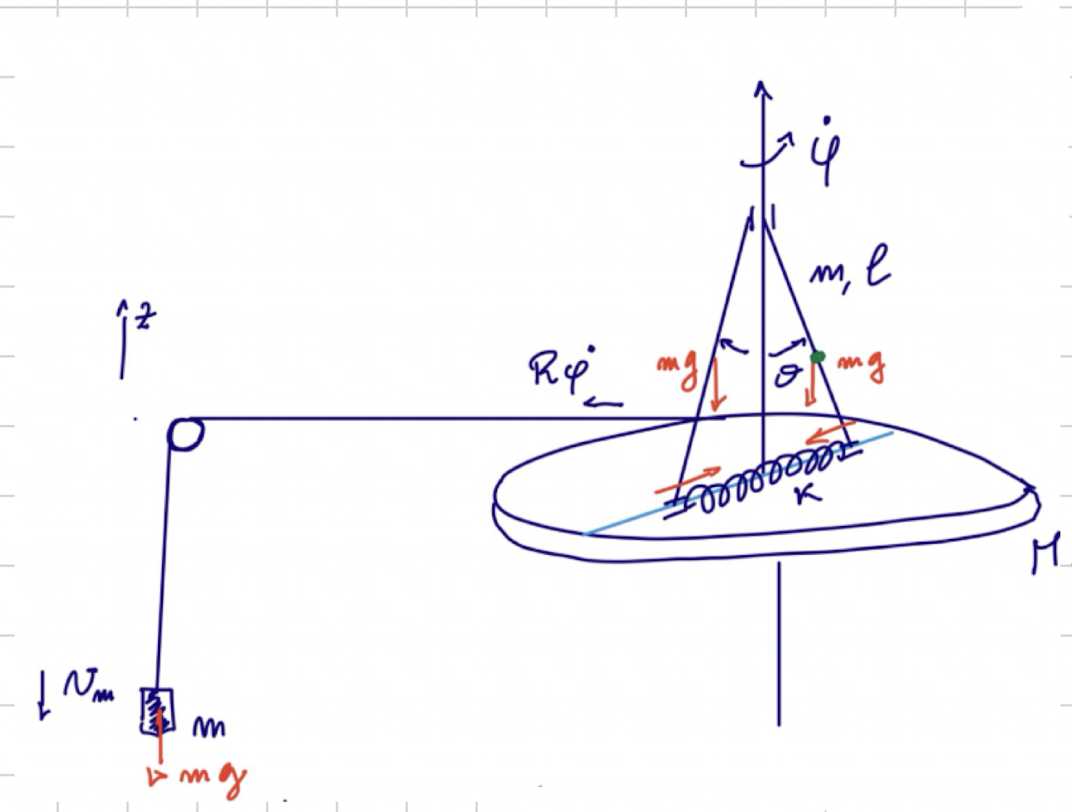
\includegraphics[width=0.55\textwidth]{immagini/piattaforma_rotante}
\end{figure}

Il disco ha massa \(M\) e raggio \(R\), le aste hanno entrambe massa \(m\) e lunghezza \(\ell\), il peso ha massa \(m\), il filo rotola senza strisciare attorno al disco. Il disco ruota attorno ad un asse principale d'inerzia e quindi ruota in un piano fisso. La molla ha costante elastica \(k\).

Il sistema ha due gradi di libertà. Scegliamo come coordinate libere \(\varphi\), angolo di rotazione del disco, e \(\theta\), angolo in figura.

La velocità del filo è uniforme ed uguale a \(R\dot{\varphi}\) (puro rotolamento). Allora
\[
y_m=-R\varphi
\]
supponendo che \(y_m(0)=0\).

Scriviamo l'energia potenziale del sistema.

\[
V=V^m+2V^{\text{peso asta}}+V^{\text{molla}}
\]

\[
V^m=mgy_m=-mgR\varphi
\]

\[
V^{\text{peso asta}}
=
mg\frac{\ell}{2}\cos\theta
\]

\[
V^{\text{molla}}
=
\frac{k}{2}\left(2\ell\sin\theta\right)^2
=
\frac{k}{2}4\ell^2\sin^2\theta
=
2k\ell^2\sin^2\theta
\]

\[
V
=
-mgR\varphi
+
2mg\frac{\ell}{2}\cos\theta
+
2k\ell^2\sin^2\theta
=
-mgR\varphi
+
mg\ell\cos\theta
+
2k\ell^2\sin^2\theta
\]

Calcoliamo ora l'energia cinetica

\[
T=T^{\text{disco}}+2T^{\text{asta}}+T^m
\]

\[
T^{\text{disco}}
=
\frac{MR^2}{2}\frac{\dot{\varphi}^2}{2}
\]

\[
T^m
=
\frac{m}{2}\dot{y}_m^2
=
\frac{m}{2}R^2\dot{\varphi}^2
\]

\[
T^{\text{asta}}
=
\frac{mv_G^2}{2}
+
\frac{\underline{\omega}_G I_G \underline{\omega}_G}{2}
\]

\(I_G\), \(\underline{\omega}\) rappresentati nelle componenti principali d'inerzia.
Partiamo dalla velocità del centro di massa.
\begin{center}
\begin{tikzpicture}[scale=1.2,>=Latex]

% punti principali
\coordinate (O) at (0,0);
\coordinate (P) at (0,2.9);
\coordinate (L) at (-1.2,0.75);
\coordinate (R) at (1.05,0.75);
\coordinate (G) at (-0.58,1.86);

% asse verticale
\draw[thick,->] (0,-1.4) -- (0,3.65) node[above] {$\hat z$};

% freccia che gira attorno all'asse verticale
\draw[thick,->]
  (0.38,3.15)
  arc[start angle=20,end angle=320,x radius=0.38,y radius=0.16];
\node[right] at (0.42,3.18) {$\dot{\varphi}$};

% aste
\draw[thick] (P) -- (L);
\draw[thick] (P) -- (R);

% centro di massa
\fill (G) circle (1.8pt);
\node[left] at (G) {$G$};

% graffa per l/2
\draw[
  thick,
  decorate,
  decoration={brace,amplitude=5pt}
]
  ($(G)+(-0.08,0.03)$) -- ($(P)+(-0.08,0.03)$)
  node[midway,left=3pt] {$\dfrac{\ell}{2}$};

% angolo theta
\draw[thick]
  ($(P)+(270:0.48)$)
  arc[start angle=270,end angle=300,radius=0.48];
\node[right] at ($(P)+(266:0.68)$) {$\theta$};

% terna locale rossa
\coordinate (A) at (0.55,1.82);

% asse k
\draw[->,red,thick] (A) -- ++(0,0.72) node[above] {$\hat{k}$};

% asse n
\draw[->,red,thick] (A) -- ++(0.95,0) node[right] {$\hat{n}$};

% asse t entrante: cerchietto con x
\draw[red,thick] (A) circle (0.12);
\draw[red,thick] ($(A)+(-0.07,-0.07)$) -- ($(A)+(0.07,0.07)$);
\draw[red,thick] ($(A)+(-0.07,0.07)$) -- ($(A)+(0.07,-0.07)$);
\node[red,below left] at ($(A)+(-0.02,-0.02)$) {$\hat{t}$};

\end{tikzpicture}
\end{center}

\[
\underline{v}_G
=
\left(
\frac{\ell}{2}\sin\theta\,\dot{\varphi}
\right)\hat{t}
+
\dot{x}_G\hat{n}
+
\dot{z}_G\hat{k}
\]

\[
x_G=\frac{\ell}{2}\sin\theta
\qquad
z_G=\frac{\ell}{2}\cos\theta
\qquad
\Rightarrow
\qquad
\dot{x}_G=\dot{\theta}\frac{\ell}{2}\cos\theta
\qquad
\dot{z}_G=-\frac{\ell}{2}\dot{\theta}\sin\theta
\]

\[
\Rightarrow
\frac{m}{2}v_G^2
=
\left(
\frac{\ell^2}{4}\dot{\theta}^2
+
\frac{\ell^2}{4}\sin^2\theta\,\dot{\varphi}^2
\right)
\frac{m}{2}
=
\frac{m}{2}\frac{\ell^2}{4}
\left(
\dot{\theta}^2+\sin^2\theta\,\dot{\varphi}^2
\right)
\]

Passiamo ora alla parte rotazionale. Sia
\[
\{\hat{i}',\hat{j}',\hat{k}'\}
\]
una base ortonormale destrosa diretta lungo gli assi principali d'inerzia. Rispetto a questa base il tensore d'inerzia è rappresentato tramite una matrice diagonale

\[
I_G=
\begin{pmatrix}
\displaystyle \int y^2+z^2\,dm & 0 & 0\\[1.2em]
0 & \displaystyle \int x^2+z^2\,dm & 0\\[1.2em]
0 & 0 & \displaystyle \int x^2+y^2\,dm
\end{pmatrix}
\]

Ora dal momento che stiamo modellizzando l'asta come un oggetto monodimensionale di massa uniformemente distribuita possiamo definire una densità lineare
\[
\lambda=\frac{m}{\ell}
\]
tale per cui
\[
dm=\lambda\,d\ell.
\]
Allora detta
\[
\gamma:\left[-\frac{\ell}{2},\frac{\ell}{2}\right]\to\mathbb{R}^3
\qquad
\gamma(t)=(0,0,t)
\]

\[
\begin{aligned}
I_x
&=
\int_{\gamma}
\left.
\left(y^2+z^2\right)
\right|_{(x,y,z)=\gamma(t)}
\cdot \lambda\,d\ell
\\
&=
\int_{-\frac{\ell}{2}}^{\frac{\ell}{2}}
t^2\lambda\,dt
=
\lambda
\int_{-\frac{\ell}{2}}^{\frac{\ell}{2}}
t^2\,dt
=
\lambda
\left[
\frac{t^3}{3}
\right]_{-\frac{\ell}{2}}^{\frac{\ell}{2}}
\\
&=
\lambda\frac{\ell^3}{8}\cdot\frac{1}{3}
+
\lambda\frac{\ell^3}{8}\cdot\frac{1}{3}
=
\frac{\lambda\ell^3}{12}
=
\frac{m\ell^2}{12}.
\end{aligned}
\]
\[
I_y
=
\int_{\gamma}
\left(x^2+z^2\right)\lambda\,d\ell
=
\int_{-\frac{\ell}{2}}^{\frac{\ell}{2}}
t^2\lambda\,dt
=
\frac{m\ell^2}{12}
\]

\[
I_z
=
\int_{\gamma}
\left(x^2+y^2\right)\lambda\,d\ell
=
\int_{-\frac{\ell}{2}}^{\frac{\ell}{2}}
0\cdot \lambda\,dt
=
0
\]

\begin{center}
\begin{tikzpicture}[scale=1.28,>=Latex]

% punti principali
\coordinate (O) at (0,0);              % punto sull'asse z
\coordinate (A) at (1.45,-0.10);       % centro della terna rossa

% asse dell'asta nera (passa per A)
\coordinate (RodL) at ($(A)+(145:1.80)$);
\coordinate (RodR) at ($(A)+(-35:2.35)$);

% asse z fisso
\draw[->,thick] (0,-2.55) -- (0,3.20) node[above] {$z$};

% asta nera
\draw[thick] (RodL) -- (RodR);

% verticale tratteggiata sotto A
\draw[thick,dashed] (A) -- ++(0,-2.05);

% assi principali in rosso
\draw[->,red,thick] (A) -- ++(90:1.18) node[above] {$\hat{k}$};

% k' lungo l'asta verso alto-sinistra
\draw[->,red,thick] (A) -- ++(145:1.40) node[above left] {$\hat{k}'$};

% i' perpendicolare a k'  (145° - 90° = 55°)
\draw[->,red,thick] (A) -- ++(55:1.42) node[above right] {$\hat{i}'$};

% j' entrante
\draw[red,thick] (A) circle (0.14);
\draw[red,thick] ($(A)+(-0.085,-0.085)$) -- ($(A)+(0.085,0.085)$);
\draw[red,thick] ($(A)+(-0.085,0.085)$) -- ($(A)+(0.085,-0.085)$);
\node[red,below left] at ($(A)+(-0.03,-0.03)$) {$\hat{j}'$};

%-----------------------------------
% angolo theta a sinistra tra z e asta
%-----------------------------------
\draw[thick]
  ($(O)+(270:-0.30)$)
  arc[start angle=270,end angle=325,radius=0.58];
\node[font=\scriptsize] at ($(O)+(230:-0.25)$) {$\theta$};

%-----------------------------------
% angolo theta tra k e k'
%-----------------------------------
\draw[thick]
  ($(A)+(90:0.55)$)
  arc[start angle=90,end angle=145,radius=0.55];
\node[font=\scriptsize] at ($(A)+(118:0.76)$) {$\theta$};

%-----------------------------------
% angolo pi/2 - theta tra k e i'
%-----------------------------------
\draw[thick]
  ($(A)+(55:0.55)$)
  arc[start angle=55,end angle=90,radius=0.55];
\node[font=\scriptsize] at ($(A)+(70:0.90)$) {$\dfrac{\pi}{2}-\theta$};

%-----------------------------------
% angolo theta in basso tra verticale tratteggiata e asta
%-----------------------------------
\draw[thick]
  ($(A)+(270:0.52)$)
  arc[start angle=270,end angle=325,radius=0.52];
\node[font=\scriptsize] at ($(A)+(-60:0.75)$) {$\theta$};

\end{tikzpicture}
\end{center}

\[
\underline{\omega}
=
\dot{\varphi}\hat{k}
+
\dot{\theta}\hat{j}'
=
\dot{\varphi}\sin\theta\,\hat{i}'
+
\dot{\theta}\hat{j}'
+
\dot{\varphi}\cos\theta\,\hat{k}'
\]

\[
\frac{\underline{\omega}\cdot I_G\underline{\omega}}{2}
=
\frac{1}{2}
\begin{pmatrix}
\dot{\varphi}\sin\theta & \dot{\theta} & \dot{\varphi}\cos\theta
\end{pmatrix}
\begin{pmatrix}
\dfrac{m\ell^2}{12} & 0 & 0\\[0.8em]
0 & \dfrac{m\ell^2}{12} & 0\\[0.8em]
0 & 0 & 0
\end{pmatrix}
\begin{pmatrix}
\dot{\varphi}\sin\theta\\[0.4em]
\dot{\theta}\\[0.4em]
\dot{\varphi}\cos\theta
\end{pmatrix}
=
\]

\[
=
\frac{1}{2}
\frac{m\ell^2}{12}
\left(
\dot{\theta}^2+\dot{\varphi}^2\sin^2\theta
\right)
\]

\[
T^{\text{asta}}
=
\frac{m}{2}
\frac{\ell^2}{4}
\left(
\dot{\theta}^2+\sin^2\theta\,\dot{\varphi}^2
\right)
+
\frac{1}{2}
\frac{m\ell^2}{12}
\left(
\dot{\theta}^2+\dot{\varphi}^2\sin^2\theta
\right)
=
\frac{m}{2}
\frac{\ell^2}{3}
\left(
\dot{\theta}^2+\sin^2\theta\,\dot{\varphi}^2
\right)
=
\]

\[
=
\frac{m\ell^2}{6}
\left(
\dot{\theta}^2+\sin^2\theta\,\dot{\varphi}^2
\right)
\]

\[
\mathcal{L}
=
T-V
=
\frac{MR^2}{2}\frac{\dot{\varphi}^2}{2}
+
\frac{m}{2}
\left(R\dot{\varphi}\right)^2
+
m\frac{\ell^2}{3}
\left(
\dot{\theta}^2+\sin^2\theta\,\dot{\varphi}^2
\right)
+
mgR\varphi
-
2mg\frac{\ell}{2}\cos\theta
-
2k\ell^2\sin^2\theta
=
\]

\[
=
\frac{MR^2\dot{\varphi}^2}{4}
+
\frac{m}{2}
\left(R\dot{\varphi}\right)^2
+
m\frac{\ell^2}{3}
\left(
\dot{\theta}^2+\sin^2\theta\,\dot{\varphi}^2
\right)
+
mgR\varphi
-
mg\ell\cos\theta
-
2k\ell^2\sin^2\theta
\]
Scriviamo l'equazione di Lagrange associata a \(\varphi\)

\[
\frac{d}{dt}
\frac{\partial \mathcal{L}}{\partial \dot{\varphi}}
=
\frac{\partial \mathcal{L}}{\partial \varphi}
\]

\[
\frac{\partial \mathcal{L}}{\partial \dot{\varphi}}
=
\frac{MR^2}{2}\dot{\varphi}
+
mR^2\dot{\varphi}
+
\frac{m\ell^2}{3}\sin^2\theta\,2\dot{\varphi}
\]

\[
\frac{d}{dt}
\frac{\partial \mathcal{L}}{\partial \dot{\varphi}}
=
\frac{MR^2}{2}\ddot{\varphi}
+
mR^2\ddot{\varphi}
+
\frac{m\ell^2}{3}\sin^2\theta\,2\ddot{\varphi}
+
\frac{4m\ell^2}{3}\sin\theta\cos\theta\,\dot{\theta}\dot{\varphi}
\]

\[
\frac{\partial \mathcal{L}}{\partial \varphi}
=
mgR
\]

\[
\left(\frac{M}{2}+m\right)R^2\ddot{\varphi}
+
\frac{2m\ell^2}{3}\sin^2\theta\,\ddot{\varphi}
+
\frac{4}{3}m\ell^2\sin\theta\cos\theta\,\dot{\theta}\dot{\varphi}
=
mgR
\]

Scriviamo l'equazione di Lagrange associata a \(\theta\)

\[
\frac{d}{dt}
\frac{\partial \mathcal{L}}{\partial \dot{\theta}}
=
\frac{\partial \mathcal{L}}{\partial \theta}
\]

\[
\frac{\partial \mathcal{L}}{\partial \dot{\theta}}
=
2\frac{m\ell^2}{3}\dot{\theta}
\Rightarrow
\frac{d}{dt}
\frac{\partial \mathcal{L}}{\partial \dot{\theta}}
=
\frac{2}{3}m\ell^2\ddot{\theta}
\]

\[
\frac{\partial \mathcal{L}}{\partial \theta}
=
m\frac{\ell^2}{3}\,2\sin\theta\cos\theta\,\dot{\varphi}^2
+
mg\ell\sin\theta
-
4k\ell^2\sin\theta\cos\theta
\]

\[
\Rightarrow
\frac{2}{3}m\ell^2\ddot{\theta}
=
m\frac{\ell^2}{3}\,2\sin\theta\cos\theta\,\dot{\varphi}^2
+
mg\ell\sin\theta
-
4k\ell^2\sin\theta\cos\theta
\]

Abbiamo ottenuto un sistema di \(2\) EDO accoppiate che possiamo risolvere numericamente.
\end{example}

\chapter{Funzione Hamiltoniana}
\section{La trasformata di Legendre}

Sia \(f:\mathbb{R}\longrightarrow\mathbb{R}\) almeno derivabile con continuità due volte. Assumiamo inoltre che
\[
f''(x)>0 \quad \forall x\in\mathbb{R}.
\]
Questa condizione garantisce che la derivata prima
\[
f'(x) \text{ sia strettamente monotona crescente}.
\]

Possiamo allora invertire \(f'(x)\), ovvero definire
\[
x=(f')^{-1}(p) \quad \forall p\in \operatorname{Im}(f').
\]

Una possibile costruzione per la trasformata di Legendre è quella geometrica.

Fisso una pendenza \(p\) e disegno la retta \(y=px\).

\begin{center}
\begin{tikzpicture}[scale=1.1, >=Stealth]
  % assi
  \draw[->, thick] (-2.2,0) -- (3.2,0);
  \draw[->, thick] (0,-1.5) -- (0,3.2);

  % parametro della retta
  \def\p{1.3}

  % funzione convessa di esempio
  \draw[thick, domain=-0.8:2.7, samples=200]
    plot (\x,{0.6*(\x-1)^2 + 0.4});
  \node at (-0.95,2.35) {\(f\)};

  % retta y = px
  \draw[thick] (-1.1,{-1.1*\p}) -- (2.35,{2.35*\p});
  \node at (1.3,2.75) {\(y=px\)};

  % punto della funzione in cui la tangente è parallela alla retta
  % f'(x)=1.2(x-1), quindi f'(x)=p per x=1+p/1.2
  \pgfmathsetmacro{\xt}{1+\p/1.2}
  \pgfmathsetmacro{\yf}{0.6*(\xt-1)^2 + 0.4}
  \pgfmathsetmacro{\yl}{\p*\xt}

  % segmento verticale rosso tra funzione e retta
  \draw[red, thick] (\xt,\yf) -- (\xt,\yl);

  % freccia e scritta rossa
  \draw[red, thick, ->] (\xt+0.08,{(\yf+\yl)/2})
    .. controls (\xt+0.55,{(\yf+\yl)/2+0.2}) and (\xt+0.95,{(\yf+\yl)/2+0.1}) ..
    (\xt+1.15,{(\yf+\yl)/2+0.15});
  \node[red] at (\xt+1.55,{(\yf+\yl)/2+0.35}) {\(f^*(p)\)};
\end{tikzpicture}
\end{center}

Definisco
\[
f^*(p)=xp-f(x)
\]
con \(x\) tale che \(px-f(x)\) è massima ovvero
\[
f^*(p)=\sup_{x\in\mathbb{R}}\bigl(xp-f(x)\bigr).
\]

Tale valore è assunto per \(x\in\mathbb{R}\) tale che \(f'(x)=p\), ovvero
\[
x(p)=(f')^{-1}(p).
\]

Infatti dobbiamo massimizzare
\[
g(x)=xp-f(x)
\quad \Rightarrow \quad
g'(x)=p-f'(x)
\]
\[
\Rightarrow \quad
g''(x)=-f''(x).
\]
Allora
\[
g'(x)=0 \Longleftrightarrow f'(x)=p
\]
ed inoltre
\[
g''(x)<0 \quad \Rightarrow \quad x \text{ è un massimo}.
\]

Spesso la trasformata di Legendre viene quindi indicata come
\[
f^*(p)=x(p)p-f(x(p)),
\qquad
x(p)=(f')^{-1}(p).
\]

\begin{proposition}{}
Sia \(f(x)\) strettamente convessa su \(\mathbb{R}\) e almeno \(C^2(\mathbb{R})\) e sia \(f^*(p)\) la sua trasformata di Legendre, allora
\[
\frac{d f^{(*)}(p)}{dp}=x
\]
ovvero l'antitrasformata della trasformata di Legendre è la sua derivata.
\end{proposition}

\begin{proof}
\[
\frac{d f^{(*)}(p)}{dp}
=
\frac{d}{dp}\bigl(xp-f(x)\bigr)
=
\frac{dx}{dp}p+x-f'(x)\frac{dx}{dp}
=
\frac{dx}{dp}p+x-p\frac{dx}{dp}
=
x.
\]
\end{proof}

\section{Funzione di Hamilton}

Consideriamo \(\mathcal{L}(q_1,\ldots,q_m,\dot q_1,\ldots,\dot q_m)\) lagrangiana per un sistema a \(m\) gradi di libertà.
Sappiamo che possiamo scrivere le equazioni di Lagrange
\[
\frac{d}{dt}\frac{\partial \mathcal{L}}{\partial \dot q_j}
=
\frac{\partial \mathcal{L}}{\partial q_j}
\qquad
j=1,\ldots,m.
\]

Sappiamo anche che se
\[
\frac{\partial \mathcal{L}}{\partial q_j}=0
\quad \Rightarrow \quad
\frac{\partial \mathcal{L}}{\partial \dot q_j}
\]
è un integrale primo.

In generale un moto descritto nel piano delle fasi è una curva regolare

\begin{center}
\begin{tikzpicture}[scale=1.15, >=Stealth]
  \draw[->, thick] (0,0) -- (0,2.4);
  \draw[->, thick] (0,0) -- (2.4,0);
  \draw[thick] (-1.0,-1.2) -- (0,0);

  \draw[thick]
    plot[smooth, tension=0.8] coordinates {
      (-1.3,-0.8)
      (-0.9,0.0)
      (-0.25,0.55)
      (0.35,0.7)
      (0.95,0.65)
      (1.45,0.78)
      (1.9,1.05)
    };

  \node at (2.9,1.15) {\((q(t),\dot q(t))\)};
\end{tikzpicture}
\end{center}

Se però riusciamo ad usare
\[
\frac{\partial \mathcal{L}}{\partial \dot q_j}
\]
come nuova coordinata libera \(\tilde q\)
allora il moto sarebbe descritto da una curva piana

\begin{center}
\begin{tikzpicture}[scale=1.15, >=Stealth]
  \draw[->, thick] (0,0) -- (0,2.5);
  \draw[->, thick] (0,0) -- (2.5,0);
  \draw[->, thick] (0,0) -- (-1.2,-1.25);

  \node at (-0.25,2.65) {\(\tilde q\)};

  \draw[red, thick]
    plot[smooth, tension=0.9] coordinates {
      (-0.85,-1.0)
      (-0.45,-0.45)
      (0.25,-0.18)
      (0.9,0.08)
      (1.4,0.28)
      (1.65,0.55)
      (1.95,0.48)
    };

  \node at (-0.45,-1.35) {\((q(t),\dot q(t))\)};

  \draw[thick, ->]
    (1.65,0.25) .. controls (2.0,-0.05) and (2.4,0.0) .. (2.65,0.1);

  \node at (3.35,0.35) {sta nel piano};
  \node at (3.15,-0.15) {\(\dot{\tilde q}=\text{cost.}\)};
\end{tikzpicture}
\end{center}

ovvero lavoreremmo in uno spazio delle fasi di dimensione minore.

Questa è l'idea dietro la funzione di Hamilton. Come vedremo però la sua definizione non dipende da integrali primi del moto ed è quindi utilizzabile anche in casi più generali.

\begin{definition}{}
Si definisce funzione Hamiltoniana la trasformata di Legendre della lagrangiana.
\end{definition}

Se consideriamo un sistema ad \(1\) grado di libertà siamo già pronti a scrivere l'Hamiltoniana.
\[
\mathcal{L}=\mathcal{L}(q,\dot q)
\qquad
\text{definisco}
\qquad
p=\frac{\partial \mathcal{L}}{\partial \dot q}
\qquad
\text{allora}
\]
\[
H(p,q)=p\dot q(p,q)-\tilde{\mathcal{L}}(q,p)
\]
avendo definito
\[
\tilde{\mathcal{L}}(q,p)=\mathcal{L}(q,\dot q(q,p)).
\]

Possiamo generalizzare la definizione al caso con \(m\) gradi di libertà ma prima facciamo un'osservazione \((\text{valida anche per }m=1)\).
\begin{oss}{}
\(\mathcal{L}\) è una funzione convessa di \(\dot q\).
\[
\mathcal{L}
=
T(\underline q,\dot{\underline q})-V(\underline q)
=
\frac{1}{2}\sum_{i=1}^{n}m_i\,\underline v_i\cdot \underline v_i
-
V(\underline q)
=
\frac{1}{2}\sum_{i=1}^{n}m_i\,
\frac{d\underline x_i}{dt}\cdot \frac{d\underline x_i}{dt}
-
V(\underline q)
=
\]
\[
=
\frac{1}{2}\sum_{i=1}^{n}
\left[
m_i
\left(
\sum_{j=1}^{m}\frac{\partial \underline x_i}{\partial q_j}\dot q_j
\right)
\left(
\sum_{k=1}^{m}\frac{\partial \underline x_i}{\partial q_k}\dot q_k
\right)
\right]
-
V(\underline q)
=
\frac{1}{2}\sum_{j=1}^{m}\sum_{k=1}^{m}
\left(
\sum_{i=1}^{n}m_i
\frac{\partial \underline x_i}{\partial q_j}\cdot
\frac{\partial \underline x_i}{\partial q_k}
\right)
\dot q_j\dot q_k -V(\underline{q})
=
\]
\[
=
\frac{1}{2}\sum_{j=1}^{m}\sum_{k=1}^{m}
a_{jk}\dot q_j\dot q_k
-
V(\underline q)
=
\frac{1}{2}\dot{\underline q}^{T}\underline a\,\dot{\underline q}
-
V(\underline q).
\]

Dal momento che
\[
T=
\frac{1}{2}\dot{\underline q}^{T}\underline a\,\dot{\underline q}\ge 0
\qquad
\text{e}
\qquad
T=0 \Longleftrightarrow \dot{\underline q}^{T}=\underline 0
\]
allora \(T\) è una forma quadratica definita positiva e \(\mathcal{L}(\underline q,\dot{\underline q})\) è una funzione convessa.

Nel caso \(m\) dimensionale la buona definizione dell'Hamiltoniana non dipende tanto dalla convessità di \(\mathcal{L}\) ma più dal fatto che quest'ultima è una forma quadratica definita positiva.

Definiamo
\[
p_j=
\frac{\partial \mathcal{L}}{\partial \dot q_j}
=
\frac{\partial T}{\partial \dot q_j}
\]
perché \(V(q)\) non dipende da \(\dot q_j\). Allora
\[
\underline p
=
(p_j)_{j=1,\ldots,m}
=
\nabla_{\dot{\underline q}}
\left(
\frac{1}{2}\dot{\underline q}^{T}\underline a\,\dot{\underline q}
\right)
=
\underline a\,\dot{\underline q}.
\]

Ovvero la mappa
\[
\dot{\underline q}\longmapsto \underline p
\]
è un'applicazione lineare di matrice \(\underline a\).
A questo punto usiamo il fatto che \(T\) è definita positiva e quindi ha autovalori reali positivi che garantiscono l'invertibilità.
\end{oss}
Per un sistema a \(m\) coordinate libere possiamo scrivere
\[
\mathcal{L}
=
\mathcal{L}(q_1,\ldots,q_m,\dot q_1,\ldots,\dot q_m)
=
\mathcal{L}(\underline q,\dot{\underline q})
\]
e
\[
H(\underline q,\underline p)
=
\underline p\cdot \dot{\underline q}(\underline q,\underline p)
-
\tilde{\mathcal{L}}(\underline q,\underline p)
=
\sum_{j=1}^{m}p_j\dot q_j
-
\tilde{\mathcal{L}}(q_1,\ldots,q_m,p_1,\ldots,p_m)
\]
con \(\underline p\) definito sopra e
\[
\tilde{\mathcal{L}}(\underline q,\underline p)
=
\mathcal{L}(\underline q,\dot{\underline q}(\underline q,\underline p)).
\]

Calcoliamo ora il differenziale di \(H(q,p)\) che ricordiamo agisce sullo spazio tangente.
Partiamo dal caso \(m=1\)
\[
\nabla H(q,p)
\binom{\delta q}{\delta p}
=
\begin{pmatrix}
\dfrac{\partial H}{\partial q} & \dfrac{\partial H}{\partial p}
\end{pmatrix}^{T}
\cdot
\binom{\delta q}{\delta p}
=
-\frac{\partial}{\partial q}\bigl(\tilde{\mathcal{L}}(q,p)\bigr)\cdot\delta q
+
\frac{\partial}{\partial q}\bigl(p\dot q(p,q)\bigr)\cdot\delta q
+
\]
\[
+
\frac{\partial}{\partial p}\bigl(p\dot q(p,q)\bigr)\delta p
-
\frac{\partial}{\partial p}\bigl(\tilde{\mathcal{L}}(q,p)\bigr)\delta p
=
\]
\[
=
-\frac{\partial}{\partial q}\bigl(\mathcal{L}(q,\dot q(q,p))\bigr)\cdot\delta q
+
p\frac{\partial \dot q}{\partial q}\cdot\delta q
+
\dot q(p,q)\delta p
+
p\frac{\partial \dot q}{\partial p}\delta p
-
\frac{\partial}{\partial p}\bigl(\mathcal{L}(q,\dot q(q,p))\bigr)\cdot\delta p
=
\]
\[
=
-\frac{\partial\mathcal{L}}{\partial q}\delta q
-
\frac{\partial\mathcal{L}}{\partial \dot q}\cdot
\frac{\partial\dot q}{\partial q}\cdot\delta q
+
p\frac{\partial\dot q}{\partial q}\cdot\delta q
+
\dot q\cdot\delta p
+
p\frac{\partial\dot q}{\partial p}\delta p
-
\frac{\partial\mathcal{L}}{\partial \dot q}\cdot
\frac{\partial\dot q}{\partial p}\cdot\delta p
\]

Ricordando che
\[
\frac{\partial\mathcal{L}}{\partial \dot q}=p
\]
\[
\nabla H(q,p)
\binom{\delta q}{\delta p}
=
-\frac{\partial\mathcal{L}}{\partial q}\cdot\delta q
-
p\cdot\frac{\partial\dot q}{\partial q}\cdot\delta q
+
p\frac{\partial\dot q}{\partial q}\cdot\delta q
+
\dot q\delta p
+
p\frac{\partial\dot q}{\partial p}\delta p
-
p\cdot\frac{\partial\dot q}{\partial p}\delta p
=
\]
\[
=
-\frac{\partial\mathcal{L}}{\partial q}\delta q
+
\dot q\delta p
\]

Uso l'equazione di Lagrange
\[
\frac{d}{dt}\frac{\partial\mathcal{L}}{\partial \dot q}
=
\dot p
=
\frac{\partial\mathcal{L}}{\partial q}
\]
\[
\nabla H(q,p)
=
-\dot p\delta q+\dot q\delta p
\]

Dal momento che è valido \(\forall \delta q,\delta p\) allora ottengo le equazioni di Hamilton
\[
\begin{cases}
\dot q=\dfrac{\partial H}{\partial p}\\[6pt]
\dot p=-\dfrac{\partial H}{\partial q}
\end{cases}
\]


Nel caso a \(m\) gradi di libertà con passaggi analoghi dall'Hamiltoniana
\[
H(\underline q,\underline p)
=
\underline p\cdot \dot{\underline q}(\underline q,\underline p)
-
\tilde{\mathcal{L}}(\underline q,\underline p)
\]
si ottengono le equazioni di Hamilton
\[
\begin{cases}
\dot q_j=\dfrac{\partial H}{\partial p_j}\\[6pt]
\dot p_j=-\dfrac{\partial H}{\partial q_j}
\end{cases}
\qquad
\forall j=1,\ldots,m.
\]

Rispetto alle equazioni di Lagrange siamo passati da \(m\) equazioni del secondo ordine a \(2m\) equazioni del primo ordine.

\begin{oss}{}
\(m=1\)
\[
\begin{cases}
\dot q=\dfrac{\partial H}{\partial p}\\[6pt]
\dot p=-\dfrac{\partial H}{\partial q}
\end{cases}
\qquad
\binom{\dot q}{\dot p}
=
\begin{pmatrix}
0 & 1\\
-1 & 0
\end{pmatrix}
\binom{\dfrac{\partial H}{\partial q}}{\dfrac{\partial H}{\partial p}}
\]

La matrice
\[
\begin{pmatrix}
0 & 1\\
-1 & 0
\end{pmatrix}
\]
è detta matrice simplettica.
\end{oss}

\begin{oss}{}
Se
\[
\mathcal{L}=\mathcal{L}(\underline q,\dot{\underline q}_j,t)
\]
dipende anche dal tempo allora anche
\[
H=H(\underline q,\underline p,t)
\]
dipenderà dal tempo e allo stesso modo si possono ricavare equazioni di Hamilton modificate.
\end{oss}

\begin{oss}{}
Se un sistema è conservativo \(H\) è l'energia totale \(H(q,p)\).

Dimostriamo il caso \(m=1\). Sappiamo che
\[
T=\frac{1}{2}a(q)\dot q^2,
\qquad
a>0,
\qquad
\mathcal{L}=\frac{1}{2}a(q)\dot q^2-V(q),
\qquad
p=\frac{\partial\mathcal{L}}{\partial\dot q}
=
a(q)\dot q.
\]
\[
\Rightarrow
H
=
p\dot q-\mathcal{L}(q,\dot q)
=
p\cdot\frac{p}{a(q)}
-
\mathcal{L}\left(q,\frac{p}{a(q)}\right)
=
p\cdot\frac{p}{a(q)}
-
\frac{1}{2}a(q)\dot q^2
+
V(q)
=
\frac{p^2}{a(q)}
-
\frac{1}{2}a(q)\frac{p^2}{a^2(q)}
+
V(q)
=
\]
\[
=
\frac{1}{2}\frac{p^2}{a(q)}
+
V(q)
=
\frac{1}{2}a(q)\dot q^2+V(q)
=
T+V.
\]
\end{oss}


\begin{example}{}
Oscillatore armonico
\[
m\ddot{x}=-Kx
\]
\[
T=\frac{m\dot{x}^2}{2}
\qquad
V=\frac{Kx^2}{2}
\qquad
q=x
\quad \Rightarrow \quad
\mathcal{L}=\frac{m\dot{x}^2}{2}-\frac{Kx^2}{2}
\]
\[
p=\frac{\partial \mathcal{L}}{\partial \dot{x}}=m\dot{x}
\]
\[
H(p,q)
=
\frac{m\dot{x}^2}{2}
+
\frac{Kx^2}{2}
=
\frac{mp^2}{2m^2}
+
\frac{Kx^2}{2}
=
\frac{p^2}{2m}
+
\frac{Kx^2}{2}
\]
\end{example}

\begin{example}{}
Consideriamo un punto materiale di massa \(m\) soggetto al vincolo
\[
y=\frac{x^2}{2}.
\]

\begin{center}
\begin{tikzpicture}[scale=1.1, >=Stealth]
  % assi
  \draw[thick] (-2.2,0) -- (2.8,0);
  \draw[thick] (0,-0.8) -- (0,2.5);

  % parabola
  \draw[thick, domain=-1.75:1.9, samples=200]
    plot (\x,{0.5*\x*\x});

  \node at (1.8,1.95) {\(y=\dfrac{x^2}{2}\)};

  % punto materiale
  \fill[black] (-1.35,{0.5*1.35*1.35}) circle (1.4pt);

  % forza peso
  \draw[red, thick, ->] (-1.35,{0.5*1.35*1.35}) -- (-1.35,0.15);
  \node[red] at (-1.65,0.65) {\(mg\)};
  \draw[red, thick] (-1.75,0.15) -- (-1.25,0.15);
\end{tikzpicture}
\end{center}

Scelgo come coordinata libera \(s(t)\)
\[
\begin{cases}
x=s(t)\\[4pt]
y=\dfrac{s^2(t)}{2}
\end{cases}
\Rightarrow
\begin{cases}
\dot{x}=\dot{s}\\[4pt]
\dot{y}=\dfrac{2s\dot{s}}{2}=s\dot{s}
\end{cases}
\]
\[
\Rightarrow
T
=
\frac{1}{2}m\dot{\underline{x}}\cdot\dot{\underline{x}}
=
\frac{1}{2}m(\dot{x}^2+\dot{y}^2)
=
\frac{1}{2}m(\dot{s}^2+s^2\dot{s}^2)
=
\frac{1}{2}m\dot{s}^2(1+s^2)
\]
\[
V=mgy=mg\frac{s^2}{2}
\Rightarrow
\mathcal{L}
=
m(1+s^2)\frac{\dot{s}^2}{2}
-
mg\frac{s^2}{2}.
\]

Costruiamo l'equazione di Lagrange.
\[
\frac{\partial\mathcal{L}}{\partial\dot{s}}
=
m(1+s^2)\dot{s}
\Rightarrow
\frac{d}{dt}\frac{\partial\mathcal{L}}{\partial\dot{s}}
=
m\ddot{s}(1+s^2)+m\dot{s}\cdot s\cdot 2\dot{s}
=
m\ddot{s}(1+s^2)+2ms\dot{s}^2
\]
\[
\frac{\partial\mathcal{L}}{\partial s}
=
m\dot{s}^2s-mgs
\Rightarrow
m(1+s^2)\ddot{s}+s\dot{s}^2m=-mgs
\Rightarrow
(1+s^2)\ddot{s}+s\dot{s}^2=-gs
\]

Come sempre siamo arrivati ad un'equazione pura del moto del secondo ordine.
Proviamo l'approccio con le equazioni di Hamilton
\[
p=
\frac{\partial\mathcal{L}}{\partial\dot{s}}
=
m(1+s^2)\dot{s}
\Rightarrow
\dot{s}
=
\frac{p}{m(1+s^2)}
\]

In questo caso è stato possibile esplicitare un'equazione già da subito.
Questo non avviene in generale.
Calcoliamo l'hamiltoniana
\[
H
=
p\dot{s}-\mathcal{L}(s,\dot{s})
=
p\cdot\frac{p}{m(1+s^2)}
-
m\frac{(1+s^2)}{2}\cdot
\frac{p^2}{m^2(1+s^2)^2}
+
mg\frac{s^2}{2}
=
\frac{p^2}{2m(1+s^2)}
+
mg\frac{s^2}{2}
\]
\[
\Rightarrow
\begin{cases}
\dot{s}=\dfrac{\partial H}{\partial p}\\[6pt]
\dot{p}=-\dfrac{\partial H}{\partial s}
\end{cases}
\Rightarrow
\begin{cases}
\dot{s}=\dfrac{p}{(1+s^2)m}\\[8pt]
\dot{p}
=
-\left(
\dfrac{p^2(-2s)}{2m(1+s^2)^2}
+
mgs
\right)
=
\dfrac{p^2s}{m(1+s^2)^2}
-
mgs
\end{cases}
\]
Come previsto abbiamo ottenuto 2 equazioni del primo ordine accoppiate.
\end{example}

\chapter{Piccole oscillazioni}
\section{Linearizzazione di un sistema conservativo attorno ad una configurazione di equilibrio stabile}
\begin{example}{}
Riprendiamo lo studio del pendolo semplice.

\begin{center}
\begin{tikzpicture}[scale=1.1, >=Stealth]
  % supporto
  \fill (0,2.2) circle (1.2pt);
  \node[above] at (0,2.2) {\(O\)};
  \draw[thick] (0,2.2) -- (0,0.2);

  % pendolo
  \draw[thick] (0,2.2) -- (1.35,0.95);
  \fill (1.35,0.95) circle (2pt);
  \node[right] at (1.45,0.95) {\(m\)};

  % angolo
  \draw (0,1.75) arc[start angle=-90,end angle=-43,radius=0.45];
  \node at (0.27,1.55) {\(\theta\)};

  % velocita'
  \draw[green!60!black, thick, ->] (1.35,0.95) -- (2.1,1.35);
  \node[green!60!black] at (1.95,1.55) {\(\ell\dot{\theta}=v\)};

  % peso
  \draw[red, thick, ->] (1.35,0.95) -- (1.35,0.25);
  \node[red] at (1.7,0.45) {\(mg\)};
\end{tikzpicture}
\end{center}

Scriviamo la seconda equazione cardinale.
\[
\frac{d}{dt}(x\wedge mv)=-\ell mg\sin\theta
\Rightarrow
\frac{d}{dt}(\ell^2\dot{\theta}m)=-\ell mg\sin\theta
\Rightarrow
\ddot{\theta}=-\frac{g}{\ell}\sin\theta
\]

Se \(\theta\ll 1\Rightarrow \sin\theta\sim\theta\)

\[
\ddot{\theta}=-\frac{g}{\ell}\theta=-\omega^2\theta
\Rightarrow
\theta(t)=A\cos(\omega t+\varphi),
\qquad
\omega^2=\frac{g}{\ell}
\]

Moltiplico l'equazione per \(\dot{\theta}\)

\[
\ddot{\theta}\dot{\theta}=-\omega^2\theta\dot{\theta}
\Rightarrow
\frac{d}{dt}\left(\frac{\dot{\theta}^2}{2}\right)
=
-\frac{d}{dt}\left(\frac{\omega^2\theta^2}{2}\right)
\Rightarrow
\frac{d}{dt}\left(\frac{\dot{\theta}^2}{2}+\omega^2\frac{\theta^2}{2}\right)=0
\]

Ora notiamo che
\[
E=\frac{1}{2}m(\ell\dot{\theta})^2-mg\ell\cos\theta
=
\frac{1}{2}m\ell^2\dot{\theta}^2-mg\ell\cos\theta
\]

e linearizzando \(\cos\theta\sim 1-\frac{\theta^2}{2}\)

\[
E
=
\frac{1}{2}m\ell^2\dot{\theta}^2-mg\ell\left(1-\frac{\theta^2}{2}\right)
=
\frac{1}{2}m\ell^2\dot{\theta}^2+\frac{1}{2}mg\ell\theta^2-mg\ell
\]

\[
\frac{dE}{dt}
=
\frac{d}{dt}\left(\frac{1}{2}m\ell^2\dot{\theta}^2+\frac{1}{2}mg\ell\theta^2-mg\ell\right)
=
\frac{d}{dt}\left(\frac{1}{2}m\ell^2\dot{\theta}^2+\frac{1}{2}mg\ell\theta^2\right)
=
\]

\[
=
m\ell^2\frac{d}{dt}\left(\frac{\dot{\theta}^2}{2}+\frac{1}{2}\frac{g}{\ell}\theta^2\right)
=
m\ell^2\frac{d}{dt}\left(\frac{\dot{\theta}^2}{2}+\frac{1}{2}\omega^2\theta^2\right)=0
\]

Ritroviamo quindi la conservazione dell'energia. Nel piano delle fasi gli stati ammessi stanno sull'ellisse
\[
\frac{\dot{\theta}^2}{2}+\frac{\theta^2}{2}\omega^2=\frac{E}{m\ell^2}
\]

Nel caso del pendolo non linearizzato non so integrare
\[
\ddot{\theta}=-\omega^2\sin\theta
\]
ma so che il moto deve stare sulla curva dell'energia nel piano delle fasi in figura

\begin{center}
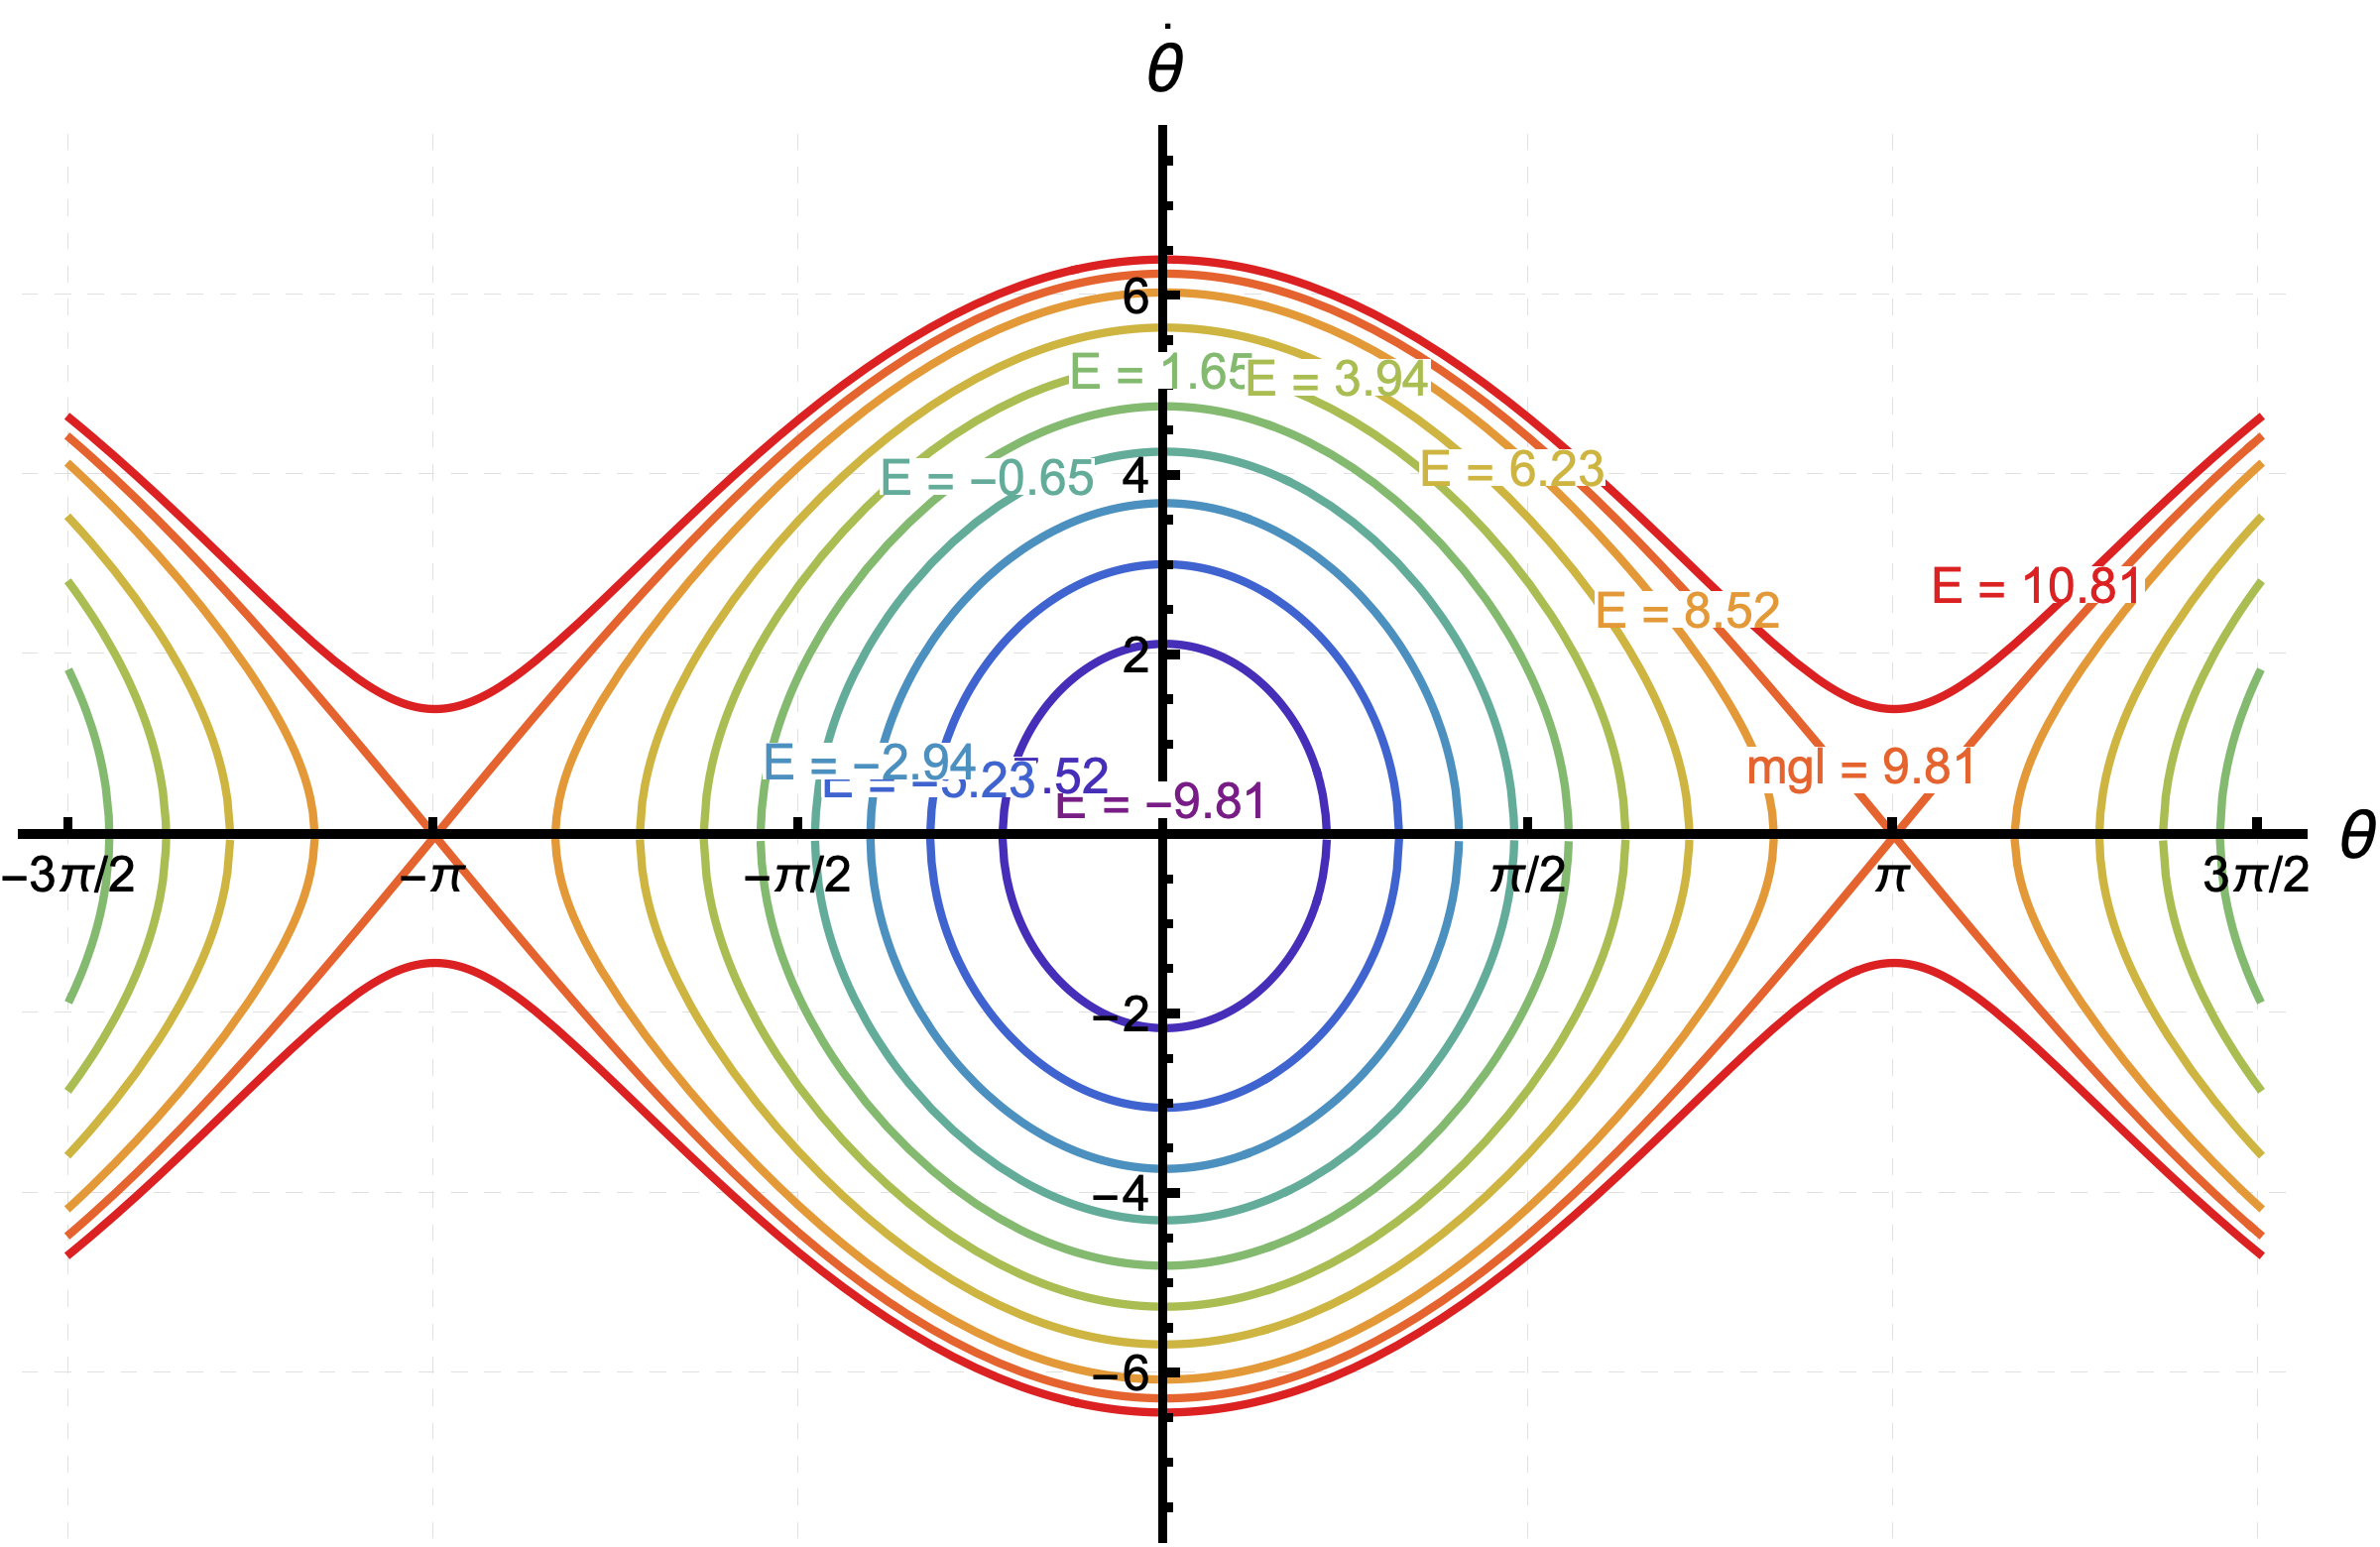
\includegraphics[width=0.62\linewidth]{immagini/grafico_pendolo}
\end{center}

La curva ad energia \(E=mg\ell\) si chiama curva separatrice

\[
E<E_0=mg\ell
\qquad
\text{orbite chiuse}
\]

\[
E>E_0=mg\ell
\qquad
\text{orbite aperte}
\]

Notiamo che il verso di percorrenza di queste curve dipende dalle condizioni iniziali. Nel piano delle fasi

\[
\begin{cases}
x=\theta\\
y=\dot{\theta}
\end{cases}
\Rightarrow
\begin{cases}
\dot{x}=\dot{\theta}\\
\dot{y}=\ddot{\theta}=-\omega^2\sin\theta
\end{cases}
\]

Allora
\[
\vec{v}=(\dot{\theta},-\omega^2\sin\theta)
\]
ovvero il segno di \(\dot{\theta}\) mi dice se mi muovo a destra o a sinistra e il segno di \(-\omega^2\sin\theta\) mi dice se mi muovo in alto o in basso.\\
Se $\dot \theta > 0 $ le curve vengono percorse verso destra mentre se $\dot \theta < 0$ vengono percorse verso sinistra. Inoltre se
\[
\sin \theta < 0 \quad \Leftrightarrow - \pi + 2k \pi < \theta < 2 k \pi
\]
le curve vengono percorse verso l'alto mentre se
\[
\sin \theta > 0 2k \pi < \theta < \pi + 2k \pi
\]
le curve vengono percorse verso il basso.\\
In conclusione se $E < mgl$ le curve chiuse vengono percorse in senso orario mentre se $E > mgl$ le curve aperte vengono percorse verso destra se $\dot \theta> 0$ e verso sinistra se $\dot \theta < 0$.\\
Analizziamo ora il periodo del pendolo. Nel caso lineare

\[
\theta\ll 1
\qquad
\sin\theta\sim\theta
\qquad
\theta(t)=A\cos(\omega t+\varphi)
\qquad
\omega^2=\frac{g}{\ell}
\Rightarrow
T=\frac{2\pi}{\omega}=2\pi\sqrt{\frac{\ell}{g}}
\]

Questa è detta isocronia delle piccole oscillazioni ed è attribuita a Galileo.

Nel caso non lineare

\[
\ddot{\theta}=-\omega^2\sin\theta
\Rightarrow
\dot{\theta}\ddot{\theta}=-\omega^2\sin\theta\dot{\theta}
\Rightarrow
\frac{d}{dt}\left(\frac{\dot{\theta}^2}{2}\right)
=
-\omega^2\frac{d}{dt}(-\cos\theta)
\]

\[
\Rightarrow
\frac{E}{m\ell^2}
=
\frac{\dot{\theta}^2}{2}-\omega^2\cos\theta
=
\left.\frac{\dot{\theta}^2}{2}\right|_{t=0}
-
\left.\omega^2\cos\theta\right|_{t=0}
\]

Chiamo
\[
\mathcal{E}=\frac{E}{m\ell^2}
\]

\[
\Rightarrow
\frac{\dot{\theta}^2}{2}=\mathcal{E}+\omega^2\cos\theta
\Rightarrow
\dot{\theta}^2=2(\mathcal{E}+\omega^2\cos\theta)
\Rightarrow
\dot{\theta}=\pm\sqrt{2}\cdot\sqrt{\mathcal{E}+\omega^2\cos\theta}
\]

Scelgo una traiettoria da \(-\theta_0\) a \(\theta_0\) e quindi \(\dot{\theta}>0\) ovvero

\[
\dot{\theta}
=
\sqrt{2}\cdot\sqrt{\mathcal{E}+\omega^2\cos\theta}
=
\frac{d\theta}{dt}
\]

Abbiamo trovato una EDO a variabili separabili. La integro tra \(0\) e \(T/2\) perché integrare da \(0\) a \(T\) implicherebbe integrare tra \(-\theta_0\) e \(-\theta_0\).

\[
\frac{d\theta}{\sqrt{2}\sqrt{\mathcal{E}+\omega^2\cos\theta}}=dt
\Rightarrow
\int_{0}^{T/2}dt=\frac{T}{2}
=
\int_{-\theta_0}^{\theta_0}
\frac{d\theta}{\sqrt{2}\sqrt{\mathcal{E}+\omega^2\cos\theta}}
\]

\[
\Rightarrow
T
=
\sqrt{2}
\int_{-\theta_0}^{\theta_0}
\frac{d\theta}{\sqrt{\mathcal{E}+\omega^2\cos\theta}}
\]

Per oscillazioni chiuse si ha che per \(\theta=\theta_0\), \(\dot{\theta}=0\) ovvero

\[
\mathcal{E}=-\omega^2\cos\theta_0.
\]

Sostituendo in \(T\) si ottiene

\[
T
=
\sqrt{2}
\int_{-\theta_0}^{\theta_0}
\frac{d\theta}{\sqrt{\omega^2(\cos\theta-\cos\theta_0)}}
=
\frac{\sqrt{2}}{\omega}
\int_{-\theta_0}^{\theta_0}
\frac{d\theta}{\sqrt{\cos\theta-\cos\theta_0}}
=
\sqrt{2}\sqrt{\frac{\ell}{g}}
\int_{-\theta_0}^{\theta_0}
\frac{d\theta}{\sqrt{\cos\theta-\cos\theta_0}}
\]

Nel caso lineare
\[
\cos\theta\sim 1-\frac{\theta^2}{2}
\qquad
\cos\theta_0\sim 1-\frac{\theta_0^2}{2}
\Rightarrow
\cos\theta-\cos\theta_0=\frac{\theta_0^2-\theta^2}{2}
\]

Allora

\[
T
\sim
2\sqrt{\frac{\ell}{g}}
\int_{-\theta_0}^{\theta_0}
\frac{d\theta}{\sqrt{\theta_0^2-\theta^2}}
=
2\sqrt{\frac{\ell}{g}}
\arcsin\left(\frac{\theta}{\theta_0}\right)\Big|_{-\theta_0}^{\theta_0}
\]

\[
=
2\sqrt{\frac{\ell}{g}}
\left(\arcsin(1)-\arcsin(-1)\right)
=
2\sqrt{\frac{\ell}{g}}
\left(\frac{\pi}{2}-\left(-\frac{\pi}{2}\right)\right)
,
\,
2\pi\sqrt{\frac{\ell}{g}}
\]

Ovvero abbiamo ritrovato il periodo del pendolo linearizzato.
\end{example}
Consideriamo un sistema conservativo ad \(1\) grado di libertà. Posso scrivere
\[
T=\frac{1}{2}a(q)\dot q^2
\qquad
V=V(q)
\]

Sia \((q,\dot q)=(q_0,0)\) una configurazione di equilibrio, ovvero un minimo di \(V(q)\).

Vogliamo linearizzare le equazioni del moto attorno alla configurazione di equilibrio.

Sviluppo \(V(q)\)
\[
V(q)
=
V(q_0)+V'(q_0)(q-q_0)+\frac{V''}{2}(q_0)(q-q_0)^2+o(q-q_0)^2
\]

Visto che le costanti sono arbitrarie per un potenziale pongo \(V(q_0)=0\) ed inoltre \(V'(q_0)(q-q_0)=0\) perché \(q_0\) è un punto di minimo (Fermat). Per lo stesso motivo \(V''(q_0)>0\). Allora
\[
V(q)=\frac{V''}{2}(q_0)(q-q_0)^2+o(q-q_0)^2
\]

Allo stesso modo l'energia cinetica
\[
2T=a(q)\dot q^2
=
a(q_0)\dot q^2
+
\left.
\begin{pmatrix}
a'(q)\dot q^2\\
a(q)\cdot 2\dot q
\end{pmatrix}
\right|_{(q,\dot q)=(q_0,0)}
\cdot
\binom{q-q_0}{\dot q}
\]
\[
+
\frac{1}{2}
\begin{pmatrix}
q-q_0\\
\dot q
\end{pmatrix}^{T}
\cdot
\left.
\begin{pmatrix}
a''(q)\dot q^2 & 2a'(q)\dot q\\
a'(q)\cdot 2\dot q & 2a(q)
\end{pmatrix}
\right|_{(q,\dot q)=(q_0,0)}
\cdot
\binom{q-q_0}{\dot q}
+
o\left(
\left\|
\binom{q-q_0}{\dot q}
\right\|^2
\right)
=
\]
\[
=
\frac{1}{2}
\begin{pmatrix}
q-q_0\\
\dot q
\end{pmatrix}^{T}
\cdot
\begin{pmatrix}
0 & 0\\
0 & 2a(q_0)
\end{pmatrix}
\cdot
\binom{q-q_0}{\dot q}
+
o\left(
\left\|
\binom{q-q_0}{\dot q}
\right\|^2
\right)
=
\]
\[
=
\frac{1}{2}
\begin{pmatrix}
q-q_0\\
\dot q
\end{pmatrix}^{T}
\cdot
\binom{0}{2a(q_0)\dot q}
+
o\left(
\left\|
\binom{q-q_0}{\dot q}
\right\|^2
\right)
=
\]
\[
=
a(q_0)\dot q^2
+
o\left(
\left\|
\binom{q-q_0}{\dot q}
\right\|^2
\right)
\Rightarrow
T\simeq \frac{1}{2}a(q_0)\dot q^2
\]

La lagrangiana linearizzata è quindi
\[
\tilde{\mathcal{L}}
=
\frac{1}{2}a(q_0)\dot q^2
-
\frac{V''}{2}(q_0)(q-q_0)^2
\]

Scriviamo le equazioni di Lagrange del problema linearizzato
\[
\frac{\partial \tilde{\mathcal{L}}}{\partial \dot q}
=
a(q_0)\dot q
\Rightarrow
\frac{d}{dt}\frac{\partial \tilde{\mathcal{L}}}{\partial \dot q}
=
a(q_0)\ddot q,
\qquad
\frac{\partial \tilde{\mathcal{L}}}{\partial q}
=
-
V''(q_0)(q-q_0)
\]
\[
\Rightarrow
a(q_0)\ddot q=-V''(q_0)(q-q_0)
\]

Ponendo \(t=q-q_0\Rightarrow \ddot t=\ddot q\) otteniamo
\[
\ddot t=-\omega^2t,
\qquad
\omega^2=\frac{V''(q_0)}{a(q_0)}
\qquad
a(q_0)>0 \text{ perché } T>0
\]

Ogni sistema ad \(1\) G.D.L. vicino ad una configurazione di equilibrio stabile si comporta come un oscillatore armonico.
Linearizziamo ora le equazioni del moto per un sistema conservativo con \(m\) gradi di libertà.
Siano \(\{q_1,\ldots,q_m\}\) le coordinate libere.

Per il sistema possiamo scrivere
\[
V(\underline q),
\qquad
T(\underline q,\dot{\underline q})
=
\frac{1}{2}\dot{\underline q}^{T}A(\underline q)\dot{\underline q}
\qquad
\text{con } A(\underline q) \text{ definita positiva}
\]
sia
\[
(\underline q,\dot{\underline q})=(\underline q_0,\underline 0)
\]
configurazione di equilibrio stabile.

Scriviamo lo sviluppo di Taylor per \(V(\underline q)\)
\[
V(\underline q)
=
V(\underline q_0)
+
\nabla V\big|_{\underline q_0}\cdot(\underline q-\underline q_0)
+
\frac{1}{2}(\underline q-\underline q_0)^{T}
H(V)\big|_{\underline q_0}\cdot(\underline q-\underline q_0)
+
o\left(\|\underline q-\underline q_0\|^2\right)
\]

Per gli stessi motivi del caso \(m=1\) possiamo porre \(V(\underline q_0)=0\) e
\[
\nabla V(\underline q_0)=\underline 0.
\]
Inoltre \(H_V(\underline q_0)\) è definita positiva.

Con ragionamenti analoghi al caso \(m=1\) otteniamo
\[
T\sim \frac{1}{2}\dot{\underline q}^{T}A(\underline q_0)\dot{\underline q}
\]
con \(A(\underline q_0)\) definita positiva.

Poniamo $\underline{t} = \underline{q} - \underline{q_0}$. La lagrangiana per il sistema è
\[
\tilde{\mathcal{L}}
=
\frac{1}{2}\dot{\underline t}^{T}A\dot{\underline t}
-
\frac{1}{2}\underline t^{T}H_V\underline t
=
\sum_{i=1}^{m}\sum_{j=1}^{m}
a_{ij}(\underline t_0)\frac{\dot t_i\dot t_j}{2}
-
\sum_{i=1}^{m}\sum_{j=1}^{m}
\frac{H_{ij}}{2}t_it_j
\]

Allora
\[
\frac{\partial\tilde{\mathcal{L}}}{\partial\dot t_j}
=
\sum_{i=1}^{m}a_{ij}\big|_{\underline t_0}\cdot\dot t_i
\qquad
\frac{d}{dt}\frac{\partial\tilde{\mathcal{L}}}{\partial\dot t_j}
=
\sum_{i=1}^{m}a_{ij}(\underline t_0)\ddot t_i
\]
\[
\frac{\partial\tilde{\mathcal{L}}}{\partial t_j}
=
-\sum_{i=1}^{m}H_{ij}t_i
\]

\[
\Rightarrow
\sum_{i=1}^{m}a_{ij}\ddot t_i
=
-\sum_{i=1}^{m}H_{ij}t_i
\qquad
\forall j=1,\ldots,m
\]

o in forma compatta
\[
A\ddot{\underline t}=-H\underline t
\]

\[
A=\{a_{ij}\},
\qquad
H=
\left\{
\left.
\frac{\partial^2 V}{\partial t_i\partial t_j}
\right|_{\underline t_0}
\right\}
\]
sono simmetriche definite positive \(\Rightarrow\) hanno autovalori reali positivi \(\Rightarrow\) sono invertibili. Allora
\[
\ddot{\underline t}=-A^{-1}H\underline t
\]

\begin{oss}{}
Il prodotto di \(2\) matrici simmetriche non è simmetrico
\[
(AB)^{T}=B^{T}A^{T}=BA\neq AB
\]

ma vale la seguente.
\end{oss}
\begin{lemma}{}
Siano \(A, B\) simmetriche e definite positive. Allora \(AB\) è diagonalizzabile e ha autovalori reali positivi.
\end{lemma}
\begin{proof}
Consideriamo
\[
A^{-1/2}ABA^{1/2}=A^{1/2}BA^{1/2}.
\]
Si osserva che
\[
\text{(i) è simmetrica:}\quad
\left(A^{-1/2}ABA^{1/2}\right)^T
=
\left(A^{1/2}\right)^T \cdot \left(A^{-1/2}AB\right)^T
=
A^{1/2}(AB)^T\left(A^{-1/2}\right)^T
=
A^{1/2}B^TA^TA^{-1/2}
=
\]
\[
=
A^{1/2}BAA^{-1/2}
=
A^{1/2}BA^{1/2}.
\]
\[
\text{(ii) è definita positiva:}\quad
\underline{x}^T A^{-1/2}ABA^{1/2}\underline{x}
=
\underline{x}^T A^{1/2}BA^{1/2}\underline{x}
=
\underline{x}^T\left(A^{1/2}\right)^TBA^{1/2}\underline{x}
=
\]
\[
=
\left(A^{1/2}\underline{x}\right)^TBA^{1/2}\underline{x}
=
\underline{y}^TB\underline{y}\ge 0
\quad \forall \underline{y}\in \mathbb{R}^n
\]
con
\[
\underline{y}=A^{1/2}\underline{x}.
\]
Ci ricordiamo che 2 matrici simili hanno gli stessi autovalori e notiamo che
\[
\left(A^{1/2}\right)^{-1}ABA^{1/2}\sim AB.
\]
Concludiamo che \(AB\) è diagonalizzabile e ha 2 autovalori positivi.
\end{proof}

Voglio diagonalizzare
\[
A^{-1}H=B.
\]
Considero \(P\) la matrice che ha come colonne gli autovettori di \(B\), \(D\) diagonale con autovalori sulla diagonale. Vale
\[
BP=PD
\Rightarrow
P^{-1}\ddot{\underline t}=-P^{-1}B\underline t
\]

Chiamo
\[
P\underline v=\underline t
\]

\[
\Rightarrow
P^{-1}(P\ddot{\underline v})
=
-P^{-1}BP\underline v
\Rightarrow
\ddot{\underline v}
=
-D\underline v
\Longleftrightarrow
\ddot v_i=-\lambda_i v_i
\qquad
\forall i=1,\ldots,m
\]

Le \(t_i\) sono una combinazione lineare delle \(v_i\) tramite \(P\).
Sono riuscito a scrivere il moto come una combinazione di oscillatori armonici.
\begin{example}{}
Studiamo il seguente sistema per piccole oscillazioni

\[
\begin{tikzpicture}[scale=0.9]
  \draw[green!70!black, thick, ->] (-0.2,0.4) -- (0.6,0.4);

  \draw[thick] (0.35,0.4) -- (0.55,0.4);
  \draw[thick] (0.55,0.4) -- (0.65,0.55);
  \draw[thick] (0.65,0.55) -- (0.75,0.25);
  \draw[thick] (0.75,0.25) -- (0.85,0.55);
  \draw[thick] (0.85,0.55) -- (0.95,0.25);
  \draw[thick] (0.95,0.25) -- (1.05,0.55);
  \draw[thick] (1.05,0.55) -- (1.15,0.25);
  \draw[thick] (1.15,0.25) -- (1.25,0.55);
  \draw[thick] (1.25,0.55) -- (1.35,0.25);
  \draw[thick] (1.35,0.25) -- (1.45,0.4);
  \draw[thick] (1.45,0.4) -- (1.7,0.4);

  \filldraw[black] (1.9,0.4) circle (3pt);
  \node at (1.9,0.9) {$1$};
  \node at (0.95,0.8) {$K$};

  \draw[thick] (2.1,0.4) -- (2.35,0.4);
  \draw[thick] (2.35,0.4) -- (2.45,0.55);
  \draw[thick] (2.45,0.55) -- (2.55,0.25);
  \draw[thick] (2.55,0.25) -- (2.65,0.55);
  \draw[thick] (2.65,0.55) -- (2.75,0.25);
  \draw[thick] (2.75,0.25) -- (2.85,0.55);
  \draw[thick] (2.85,0.55) -- (2.95,0.25);
  \draw[thick] (2.95,0.25) -- (3.05,0.55);
  \draw[thick] (3.05,0.55) -- (3.15,0.25);
  \draw[thick] (3.15,0.25) -- (3.25,0.4);
  \draw[thick] (3.25,0.4) -- (3.55,0.4);

  \filldraw[black] (3.75,0.4) circle (3pt);
  \node at (3.75,0.9) {$2$};
  \node at (2.8,0.8) {$K$};

  \draw[->, thick] (0.7,-0.15) -- (2.0,-0.15);
  \node at (1.4,-0.35) {$x_1$};

  \draw[->, thick] (0.7,-0.8) -- (3.8,-0.8);
  \node at (2.6,-1) {$x_2$};
\end{tikzpicture}
\]

Il sistema ha 2 gradi di libertà. Scegliamo come coordinate libere \(x_1,x_2\). Scriviamo l'energia cinetica del sistema.
\[
T = m\frac{\dot{x}_1^2}{2} + m\frac{\dot{x}_2^2}{2}
=
\frac{1}{2}
(\dot{x}_1,\dot{x}_2)
\begin{pmatrix}
m & 0\\
0 & m
\end{pmatrix}
\begin{pmatrix}
\dot{x}_1\\
\dot{x}_2
\end{pmatrix}
\]
È una forma quadratica definita positiva e quindi
\[
H_T=
\begin{pmatrix}
m & 0\\
0 & m
\end{pmatrix}.
\]
Studiamo l'energia potenziale del sistema.
\[
V(x_1,x_2)=\frac{K}{2}x_1^2+\frac{K}{2}(x_2-x_1)^2
\Rightarrow
\nabla V(x_1,x_2)=
\left(
\frac{\partial V}{\partial x_1}(x_1,x_2),
\frac{\partial V}{\partial x_2}(x_1,x_2)
\right)
=
\]
\[
=
\left(
Kx_1-K(x_2-x_1),K(x_2-x_1)
\right)
\]
I punti di equilibrio stabile sono i minimi di \(V\). Annulliamo \(\nabla V(x_1,x_2)\)
\[
\begin{cases}
K(x_2-x_1)=0 \Rightarrow x_1=x_2\\
K(2x_1-x_2)=0 \Rightarrow Kx_1=0 \Rightarrow x_1=x_2=0
\end{cases}
\]
Allora \((0,0)\) è l'unico candidato di configurazione di equilibrio statico. Studiamo l'Hessiana.
\[
\frac{\partial^2 V}{\partial x_1^2}=2K
\qquad
\frac{\partial^2 V}{\partial x_2^2}=K
\qquad
\frac{\partial^2 V}{\partial x_1\partial x_2}=-K
\Rightarrow
H_V=
\begin{pmatrix}
2K & -K\\
-K & K
\end{pmatrix}
=
K
\begin{pmatrix}
2 & -1\\
-1 & 1
\end{pmatrix}
\]
Ricordiamo che se \(f\) è un'applicazione lineare e \(f(v)=\lambda v\) allora
\[
\alpha f(v)=\alpha \lambda v
\]
ovvero gli autovalori di \(\alpha f\) sono i \(\alpha \lambda_i\) con \(\lambda_i\) autovalori di \(f\). Calcoliamo gli autovalori di
\[
\begin{pmatrix}
2 & -1\\
-1 & 1
\end{pmatrix}
\]
\[
\det
\begin{pmatrix}
2-\lambda & -1\\
-1 & 1-\lambda
\end{pmatrix}
=
(2-\lambda)(1-\lambda)-1
=
2-2\lambda-\lambda+\lambda^2-1
=
\lambda^2-3\lambda+1
\]
\[
\lambda^2-3\lambda+1=0
\Leftrightarrow
\lambda=
\frac{3\pm\sqrt{9-4}}{2}
=
\frac{3\pm\sqrt{5}}{2}
\]
Gli autovalori di \(H_V\) sono quindi
\[
\lambda_1=\frac{3-\sqrt{5}}{2}K,
\qquad
\lambda_2=\frac{3+\sqrt{5}}{2}K.
\]
In particolare \(H_V\) è definita positiva in \((0,0)\) che è quindi un punto di minimo di \(V\).

Linearizziamo il problema attorno a \((0,0)\)
\[
\mathcal{L}(\underline{x},\dot{\underline{x}})
\sim
\frac{1}{2}
(\dot{x}_1,\dot{x}_2)^T
\begin{pmatrix}
m & 0\\
0 & m
\end{pmatrix}
\begin{pmatrix}
\dot{x}_1\\
\dot{x}_2
\end{pmatrix}
-
\frac{1}{2}
(x_1,x_2)
\begin{pmatrix}
2K & -K\\
-K & K
\end{pmatrix}
\begin{pmatrix}
x_1\\
x_2
\end{pmatrix}
\]
Nelle notazioni precedenti
\[
A=
\begin{pmatrix}
m & 0\\
0 & m
\end{pmatrix}
\qquad
H=
\begin{pmatrix}
2K & -K\\
-K & K
\end{pmatrix}
\]
\[
B=A^{-1}H
=
\begin{pmatrix}
\frac{1}{m} & 0\\
0 & \frac{1}{m}
\end{pmatrix}
\cdot
\begin{pmatrix}
2K & -K\\
-K & K
\end{pmatrix}
=
\begin{pmatrix}
\frac{2K}{m} & -\frac{K}{m}\\
-\frac{K}{m} & \frac{K}{m}
\end{pmatrix}
=
\frac{K}{m}
\begin{pmatrix}
2 & -1\\
-1 & 1
\end{pmatrix}
\]
Gli autovalori di \(B\) sono
\[
\lambda_1=\frac{3-\sqrt{5}}{2}\frac{K}{m},
\qquad
\lambda_2=\frac{3+\sqrt{5}}{2}\frac{K}{m}
\]
\(\lambda_{1,2}\) sono entrambe positive e sono le frequenze proprie di oscillazione attorno all'equilibrio.
\end{example}

\begin{example}{}
Tutti i vincoli sono di puro scivolamento. Trovare il valore minimo di \(K\) perché il sistema resti in equilibrio.

\[
\begin{tikzpicture}[scale=1]
  \draw[thick] (-2.4,0) -- (2.4,0);

  \draw[thick] (-0.8,0.8) circle (0.8);
  \draw[thick] (0.8,0.8) circle (0.8);
  \draw[thick] (0,2.185) circle (0.8);


  \node at (-1.9,0.95) {\(m,r\)};
  \node at (1.9,0.95) {\(m,r\)};
  \node at (0.9,2.75) {\(m,r\)};

  \draw[red, thick, ->] (-0.8,0.8) -- (-0.8,-0.6);
  \node[red] at (-0.65,-0.35) {\(mg\)};

  \draw[red, thick, ->] (0.8,0.8) -- (0.8,-0.6);
  \node[red] at (0.95,-0.35) {\(mg\)};

  \draw[red, thick, ->] (0,2.185) -- (0,1.25);
  \node[red] at (0.2,1.8) {\(mg\)};

  \draw[orange, thick, ->] (-0.8,0) -- (-0.8,0.7);
  \node[orange] at (-1.05,0.45) {\(\varphi\)};

  \draw[orange, thick, ->] (0.8,0) -- (0.8,0.7);
  \node[orange] at (1.05,0.45) {\(\varphi\)};

  \draw[orange, thick, ->] (-0.4,1.45) -- (0,2.15);
  \node[orange] at (-0.55,1.85) {\(\xi\)};

  \draw[orange, thick, ->] (0.4,1.45) -- (0,2.15);
  \node[orange] at (0.55,1.85) {\(\xi\)};

  \draw[orange, thick, ->] (0,0.8) -- (-0.65,0.8);
  \node[orange] at (-0.35,1.02) {\(\psi\)};

  \draw[red, thick, ->] (-0.45,0.8) -- (0.3,0.8) ;
  \node[red] at (-0.05,1.05) {\(2Kr\)};


\end{tikzpicture}
\]

\begin{itemize}
  \item Bilancio delle forze su tutto il sistema
  \[
  2\varphi - 3mg = 0 \Rightarrow \varphi = \frac{3}{2}mg
  \]

  \item Bilancio delle forze disco 1 direzione orizzontale
  \[
  2Kr + \psi + \xi \cos \frac{\pi}{3} = 0
  \]

  \item Bilancio delle forze disco 1 direzione verticale
  \[
  \xi \sin \frac{\pi}{3} + \varphi - mg = 0
  \Rightarrow
  -mg + \frac{3}{2}mg = -\xi \sin \frac{\pi}{3}
  \Rightarrow
  \xi =
  \frac{-mg}{2\sin \frac{\pi}{3}}
  =
  -\frac{mg}{\sqrt{3}}
  \]
\end{itemize}

\[
\Rightarrow
\psi =
-2Kr - \xi \cos \frac{\pi}{3}
=
-2Kr + \frac{mg}{\sqrt{3}}\cdot \frac{1}{2}
=
-2Kr + \frac{mg}{2\sqrt{3}}
\]

\[
\text{Se } \psi = 0
\Rightarrow
2K_{\min}r = \frac{mg}{2\sqrt{3}}
\Rightarrow
K_{\min} = \frac{mg}{4\sqrt{3}r}
\]
\end{example}

\chapter{Tautocrona}
Possiamo vedere il pendolo come un punto che scorre su una guida circolare liscia soggetto alla forza peso

La frequenza di oscillazione del pendolo è dipendente dai dati iniziali ovvero dall'energia.

Ci domandiamo se esiste una curva non circolare che assicura una frequenza di oscillazione indipendente dai dati iniziali. Questa curva è una cicloide ribaltata. Costruiamo una sua parametrizzazione. La cicloide è la traiettoria percorsa da un punto sul bordo di un disco che si muove di puro rotolamento. Prendiamo un disco che rotola di raggio \(R\)

\[
\begin{tikzpicture}
  \draw[green!70!black, thick, ->] (-2.2,0) -- (-2.2,0.8);
  \node[green!70!black] at (-2.45,0.75) {\(\widehat{j}\)};
  \draw[green!70!black, thick, ->] (-2.2,0) -- (-1.3,0);
  \node[green!70!black] at (-1.65,-0.25) {\(\widehat{i}\)};
  \node[green!70!black] at (-2.7,0.15) {\(\widehat{k}\)};
  \draw[green!70!black] (-2.55,0.1) circle (0.12);
  \fill[green!70!black] (-2.55,0.1) circle (0.03);

  \draw[thick] (-1.2,0) -- (2.6,0);
  \draw[thick] (0,0.8) circle (0.8);
  \filldraw[black] (0,0.8) circle (1.5pt);
  \node at (-0.15,0.65) {\(G\)};
  \node at (0,-0.25) {\(C\)};

  \draw[dashed] (0,0.8) -- (0,1.6);
  \draw[thick] (0,0.8) -- (0.6,1.35);
  \filldraw[black] (0.6,1.35) circle (1.2pt);
  \node at (0.78,1.45) {\(P\)};
  \node at (0.34,1.02) {\(R\)};

  \draw[thick, ->] (-0.7,0.8) arc (180:120:0.7);
  \node at (-0.95,1.25) {\(\theta\)};
  \draw[thick, ->] (0,1.38) arc (90:66:0.58);
  \node at (0.18,1.23) {\(\theta\)};
\end{tikzpicture}
\]

\[
\underline{v}_G = R\dot{\theta}\,\widehat{i}
\qquad
\underline{v}_P =
\underline{v}_G + \omega \wedge (\underline{x}_P-\underline{x}_G)
=
R\dot{\theta}\,\widehat{i}
-
\dot{\theta}\widehat{k}\wedge
\left(R\sin\theta\,\widehat{i}+R\cos\theta\,\widehat{j}\right)
=
\]
\[
=
R\dot{\theta}\,\widehat{i}
+
R\dot{\theta}\cos\theta\,\widehat{i}
-
R\dot{\theta}\sin\theta\,\widehat{j}
\]

Integriamo ponendo \(\theta(0)=\theta_0\).

\[
\dot{x}_P = R\dot{\theta}(1+\cos\theta)
\Rightarrow
\int_0^t \dot{x}_P\,dt
=
R\int_0^t \dot{\theta}+\dot{\theta}(\cos\theta)\,dt
\Rightarrow
x_P(t)=R(\theta-\theta_0)+R\sin\theta-R\sin\theta_0
\]

\[
\dot{y}_P=-R\dot{\theta}\sin\theta
\Rightarrow
\int_0^t \dot{y}_P\,dt
=
\int_0^t -R\dot{\theta}\sin\theta\,dt
\Rightarrow
y_P(t)=R\cos\theta-R\cos\theta_0
\]

\[
\Rightarrow
\underline{x}_P(t)
=
\left(R(\theta+\sin\theta)-R(\theta_0+\sin\theta_0)\right)\widehat{i}
+
\left(R\cos\theta-R\cos\theta_0\right)\widehat{j}
\]

\[
\begin{tikzpicture}
  \draw[thick, ->] (0,-0.7) -- (0,1.9);
  \node at (-0.2,1.75) {\(y\)};
  \draw[thick, ->] (-0.7,0) -- (5.8,0);
  \node at (5.7,-0.25) {\(x\)};
  \draw[thick, domain=-0.55:5.4, samples=200, smooth]
    plot ({\x},{abs(cos(1.25*\x r))});
  \node at (2.25,0.9) {\(\underline{x}_P(t)\)};
\end{tikzpicture}
\]

Rovesciamo la curva
\[
\widetilde{\underline{x}}_P(t)
=
R(\theta+\sin\theta)\widehat{i}
-
R\cos\theta\,\widehat{j}
-
R(\theta_0+\sin\theta_0)\widehat{i}
+
R\cos\theta_0\,\widehat{j}
=
\]
\[
=
R(\theta+\sin\theta)\widehat{i}
-
R\cos\theta\,\widehat{j}
+
\underline{K},
\qquad
\underline{K}\in\mathbb{R}^2
\]

\[
\begin{tikzpicture}
  \draw[thick, ->] (0,-1.9) -- (0,1.6);
  \node at (-0.2,1.45) {\(y\)};
  \draw[thick, ->] (-0.7,0) -- (5.6,0);
  \node at (5.5,0.2) {\(x\)};
  \draw[thick, domain=-0.55:5.4, samples=200, smooth]
    plot ({\x},{-abs(cos(1.25*\x r))});
  \node at (2.25,-0.75) {\(\widetilde{\underline{x}}_P(t)\)};
\end{tikzpicture}
\]

Studio il moto di un punto nella cicloide rovesciata.

Il potenziale è
\[
V=-mgR\cos\theta+K_2
\]

Scriviamo l'energia cinetica

\[
\widetilde{\underline{v}}_P
=
R\dot{\theta}\,\widehat{i}
+
R\cos\theta\,\dot{\theta}\,\widehat{i}
+
R\dot{\theta}\sin\theta\,\widehat{j}
\Rightarrow
T=
\frac{1}{2}m\widetilde{v}_P^2
=
\left[
\left(R\dot{\theta}+R\dot{\theta}\cos\theta\right)^2
+
\left(R\dot{\theta}\sin\theta\right)^2
\right]\frac{m}{2}
=
\]
\[
=
\frac{m}{2}R^2\dot{\theta}^2
\left[
(1+\cos\theta)^2+\sin^2\theta
\right]
=
\frac{m}{2}R^2\dot{\theta}^2
\left[
2+2\cos\theta
\right]
=
mR^2\dot{\theta}^2(1+\cos\theta)
\]

\[
\mathcal{L}
=
mR^2\dot{\theta}^2(1+\cos\theta)
+
mgR\cos\theta
-
K_2
\qquad
E=
mR^2\dot{\theta}^2(1+\cos\theta)
-
mgR\cos\theta
+
K_2
\]

Ipotizzo anche \(\dot{\theta}(0)=0\). Allora

\[
E(t)=E(0)
=
mR^2\dot{\theta}^2(1+\cos\theta)
-
mgR\cos\theta
=
+K_2
-
mgR\cos\theta_0
\]

Pongo convenzionalmente \(K_2=0\)

\[
mR^2\dot{\theta}^2(1+\cos\theta)
=
mgR(\cos\theta-\cos\theta_0)
\]

Il fatto che \(\cos\theta-\cos\theta_0\ge 0 \Leftrightarrow \cos\theta\ge\cos\theta_0 \Rightarrow \theta\le\theta_0\) è coerente con il senso fisico perché se il corpo parte con velocità nulla tenderà ad invertire il suo angolo di rotazione.

\[
\dot{\theta}^2
=
\frac{g}{R}\frac{\cos\theta-\cos\theta_0}{1+\cos\theta}
\Rightarrow
\dot{\theta}
=
\sqrt{\frac{g}{R}}
\frac{\sqrt{\cos\theta-\cos\theta_0}}{\sqrt{1+\cos\theta}}
\Rightarrow
\int_{\theta_0}^0
\frac{\sqrt{1+\cos\theta}}{\sqrt{\cos\theta-\cos\theta_0}}\,d\theta
=
\int_0^{T/4}
\sqrt{\frac{g}{R}}\,dt
\]

\[
\Rightarrow
\sqrt{\frac{g}{R}}\frac{T}{4}
=
\int_{\theta_0}^{0}
\frac{\sqrt{1+\cos\theta}}{\sqrt{\cos\theta-\cos\theta_0}}
\]

Equivalentemente posso andare da \(0\) a \(\theta_0\) in \(\frac{T}{4}\)

\[
\Rightarrow
\sqrt{\frac{g}{R}}\frac{T}{4}
=
\int_0^{\theta_0}
\frac{\sqrt{1+\cos\theta}}{\sqrt{\cos\theta-\cos\theta_0}}\,d\theta
\]

Ricordiamo che
\[
\cos^2\frac{\theta}{2}
=
\frac{1+\cos\theta}{2}
\qquad
\sin^2\frac{\theta}{2}
=
\frac{1-\cos\theta}{2}
\qquad
\cos\theta
=
2\cos^2\frac{\theta}{2}-1
\]

\[
\int_0^{\theta_0}
\frac{\sqrt{1+\cos\theta}}{\sqrt{\cos\theta-\cos\theta_0}}\,d\theta
=
\int_0^{\theta_0}
\frac{\sqrt{2}\cos\frac{\theta}{2}}{\sqrt{\cos\theta-\cos\theta_0}}\,d\theta
=
\int_0^{\theta_0}
\frac{\sqrt{2}\cos\frac{\theta}{2}}{\sqrt{2\cos^2\frac{\theta}{2}-1-\left(2\cos^2\frac{\theta_0}{2}-1\right)}}\,d\theta
=
\]
\[
=
\int_0^{\theta_0}
\frac{\cos\frac{\theta}{2}}{\sqrt{\cos^2\frac{\theta}{2}-\cos^2\frac{\theta_0}{2}}}\,d\theta
\]
Poniamo $u = \sin(\theta / 2) \Rightarrow du = 1/2 \cos(\theta / 2) d \theta$. Allora 
\[
2\int_{u_1}^{u_2}
\frac{du}{\sqrt{1-\sin^2\frac{\theta}{2}-1+\sin^2\frac{\theta_0}{2}}}
=
2\int_{u_1}^{u_2}
\frac{du}{\sqrt{u_0^2-u^2}}
=
\frac{2}{u_0}
\int_{u_1}^{u_2}
\frac{du}{\sqrt{1-\left(\frac{u}{u_0}\right)^2}}
\]
Poniamo ora $v = u / u_0 \Rightarrow dv = 1/u_0 du$ ed inoltre
\[
v_1
=
\frac{u}{u_0}
=
\frac{\sin\frac{\theta}{2}}{\sin\frac{\theta_0}{2}}
\Big|_{\theta=0}
=
0
\qquad
v_2
=
\frac{u}{u_0}
=
\frac{\sin\frac{\theta}{2}}{\sin\frac{\theta_0}{2}}
\Big|_{\theta=\theta_0}
=
1
\]
Allora 
\[
2
\int_{v_1}^{v_2}
\frac{1\,dv}{\sqrt{1-v^2}}
=
2\arcsin v\Big|_{v_1}^{v_2}
=
2\arcsin v\Big|_0^1
=
\pi
\]

\[
\Rightarrow
T=
4\pi\sqrt{\frac{R}{g}}
\]
\chapter{Moltiplicatori di Lagrange e principio di Hamilton}
\section{Massimi e minimi vincolati di una funzione a valori reali}
Sia \(f:\mathbb{R}^n \to \mathbb{R}\) abbastanza liscia \(\left(\text{almeno } C^2(\mathbb{R}^n)\right)\). Voglio trovare i punti ottimi della funzione ristretta a
\[
S=\left\{\underline{x}\in\mathbb{R}^n:g(\underline{x})=0\right\}.
\]
Chiamo
\[
\widetilde{f}=f\big|_S:S\to\mathbb{R}
\qquad
\underline{x}\mapsto f(\underline{x})
\]

In generale \(\widetilde{f}\) non ha gli stessi punti critici di \(f\).

Il problema quindi diventa trovare i punti critici di \(\widetilde{f}\). Ci sono 2 possibilità

\[
\text{i) il vincolo è esprimibile come}
\]
\[
x_1=\widetilde{g}(x_2,\ldots,x_n)
\]

In questo caso posso cercare in modo standard gli ottimi della funzione
\[
\widetilde{f}:\mathbb{R}^{n-1}\to\mathbb{R}
\qquad
(x_2,\ldots,x_n)\mapsto f(x_1(x_2,\ldots,x_n),x_2,\ldots,x_n)
\]

\[
\text{ii) in generale posso cercare i punti critici della funzione}
\]
\[
f_\lambda(x_1,\ldots,x_n,\lambda)
=
f(x_1,\ldots,x_n,\lambda)
-
\lambda g(x_1,\ldots,x_n)
\]

Dove \(\lambda\) è detto moltiplicatore di Lagrange. Dobbiamo quindi risolvere il sistema

\[
\nabla f_\lambda=0
\Longleftrightarrow
\begin{cases}
\dfrac{\partial f}{\partial x_i}
-
\lambda
\dfrac{\partial g}{\partial x_i}
=0
\qquad \forall i=1,\ldots,n
\\[1em]
g(x_1,\ldots,x_n)=0
\end{cases}
\]

\begin{example}{}
\[
f:\mathbb{R}^2\to\mathbb{R}
\qquad
f(x,y)=x^2+by^2
\]

\[
y=ax+c
\Rightarrow
g(x,y)=y-ax-c=0
\]

\[
\text{i) ricavo } y=ax-c \text{ e sostituisco}
\]

\[
\widetilde{f}:\mathbb{R}\to\mathbb{R}
\qquad
\widetilde{f}(x,y(x))=x^2+b(ax+c)^2
\]

\[
\frac{d\widetilde{f}}{dx}
=
2x+2b(ax+c)a
=
0
\Rightarrow
\widetilde{x}
=
-\frac{abc}{1+a^2b}
\Rightarrow
\widetilde{y}
=
a\widetilde{x}+c
=
-\frac{a^2bc}{1+a^2b}+c
\]

\[
\text{(ii) } f_\lambda:\mathbb{R}^3\to\mathbb{R}
\qquad
f_\lambda=x^2+by^2-\lambda(y-ax-c)
\]

\[
\nabla f_\lambda
=
(2x+\lambda a,\ 2by-\lambda,\ -y+ax+c)
\]

\[
\Rightarrow
\begin{cases}
2x+\lambda a=0
\Rightarrow
2x+2aby=0
\Rightarrow
2x+2ab(ax+c)=0
\Rightarrow
2x+2a^2bx+2abc=0
\\
2by-\lambda=0
\Rightarrow
\lambda=2by
\\
y-ax-c=0
\Rightarrow
y=ax+c
\end{cases}
\]

\[
\Rightarrow
x=
\frac{-2abc}{2(1+a^2b)}
=
-\frac{abc}{1+a^2b}
\]

\[
\Rightarrow
y=
-\frac{a^2bc}{1+a^2b}
+c
\]
\end{example}

\subsubsection{Interpretazione geometrica dei moltiplicatori di Lagrange}
\begin{center}
    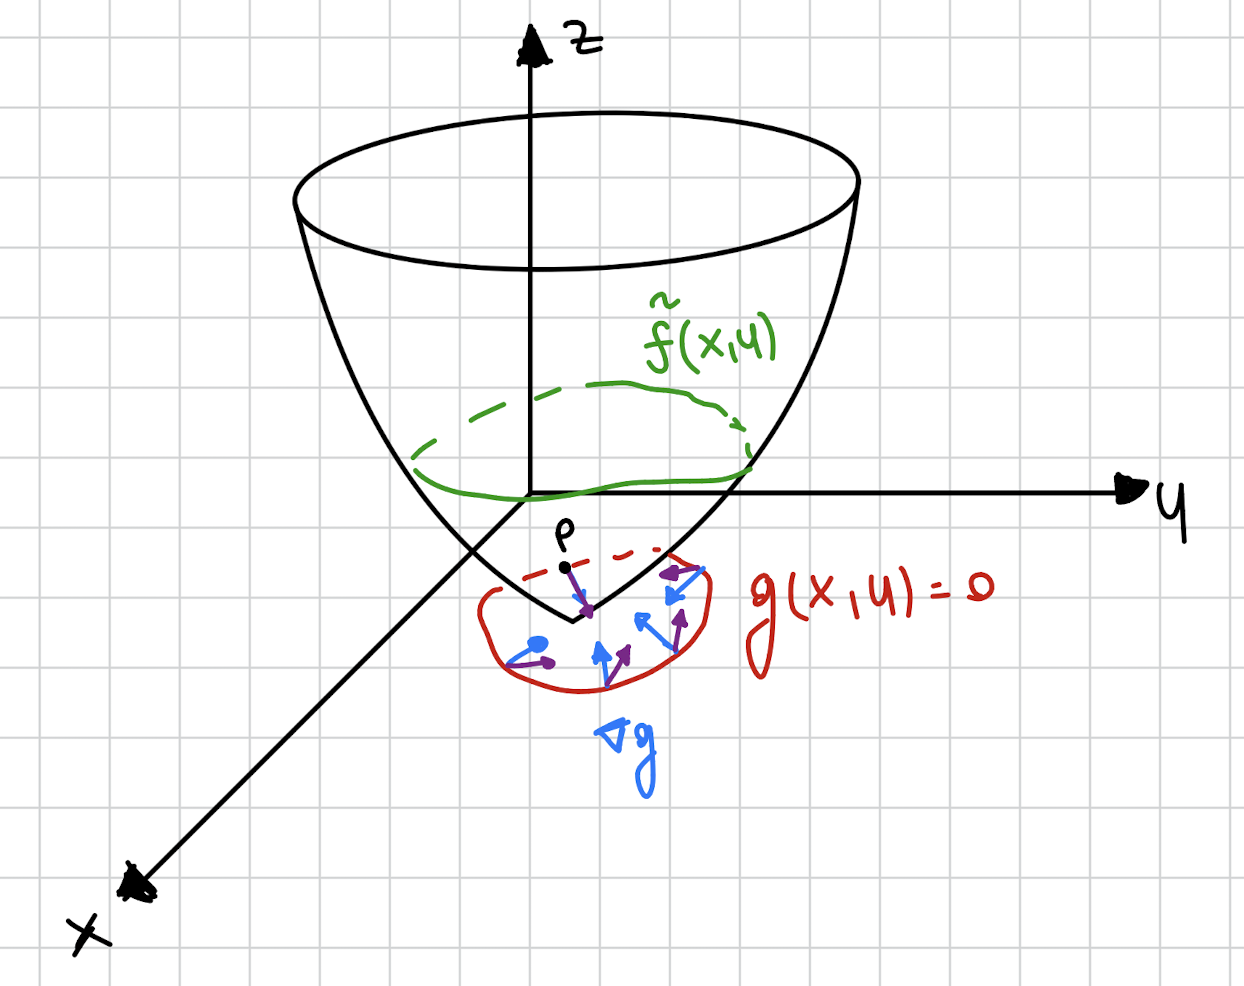
\includegraphics[scale=0.5]{immagini/molt-lagrange.png}
\end{center}

Sto chiedendo
\[
\nabla f_\lambda = \nabla f - \lambda \nabla g = 0
\Rightarrow
\nabla f = +\lambda \nabla g
\]
ovvero il minimo si ha nel punto in cui \(\nabla f\) e \(\nabla g\) sono paralleli. Infatti se così non fosse \(\nabla f\) avrebbe una componente parallela al vincolo e quindi seguendo quella direzione la funzione migliorerebbe. In figura il punto \(P\) è di ottimo.
\subsubsection{Significato fisico dei moltiplicatori di Lagrange}
Ci domandiamo che significato fisico abbia il moltiplicatore di Lagrange in un sistema meccanico.
\begin{example}{}
\[
\begin{tikzpicture}[scale=1.1]
  % piano inclinato
  \draw[thick] (-2,1.2) -- (2,-1.2);
  \draw[dashed] (-2.2,-1.2) -- (1.4,-1.2);

  % assi
  \fill[red] (-1.2,0.72) circle (1.2pt);
  \draw[->,thick] (-1.2,0.72) -- (0.2,2.35) node[above] {$y$};
  \draw[->,thick] (-1.2,0.72) -- (2.2,-1.35) node[right] {$x$};

  % disco
  \draw[thick] (0,0.82) circle (0.72);
  \node at (0.12,1.03) {$G$};

  % centro e contatto
  \fill[red] (0,-0.12) circle (1.2pt);
  \node[left] at (-0.05,-0.18) {$C$};

  % mg
  \draw[->,red,thick] (0.12,0.9) -- (0.12,0.1);
  \node[red,right] at (0.16,0.45) {$mg$};

  % forza tangenziale
  \draw[->,red,thick] (0,-0.12) -- (0.85,-0.63);
  \node[red] at (0.1,-0.55) {$F_s$};

  % angolo alpha
  \draw (1.05,-1.02) arc[start angle=180,end angle=142,radius=0.55];
  \node at (0.85,-1.0) {$\alpha$};

  % freccia theta
  \draw[->,thick] (0.62,1.42) arc[start angle=40,end angle=-35,radius=0.52];
  \node[right] at (0.98,0.95) {$\theta$};
\end{tikzpicture}
\]

Il disco è soggetto ad un puro rotolamento

\[
x_G=R\theta
\qquad
\Rightarrow
\qquad
g(x_G,\theta)=x_G-R\theta
\qquad
\Rightarrow
\qquad
g(x_G,\theta)=0
\]

\[
T=\frac{m\dot{x}_G^2}{2}+\frac{mR^2}{2}\frac{\dot{\theta}^2}{2}
\qquad
V=mg\,x_G\sin\alpha
\qquad
\mathcal{L}=\frac{m\dot{x}_G^2}{2}+\frac{mR^2}{2}\frac{\dot{\theta}^2}{2}+mg\,x_G\sin\alpha
\]

\[
\mathcal{L}_\lambda=
\frac{m\dot{x}_G^2}{2}
+
\frac{mR^2}{2}\frac{\dot{\theta}^2}{2}
+
mg\,x_G\sin\alpha
-
\lambda(x_G-R\theta)
\]

\[
\begin{cases}
\dfrac{d}{dt}\dfrac{\partial\mathcal{L}}{\partial \dot{x}_G}-\dfrac{\partial\mathcal{L}}{\partial x_G}
=
-\lambda\dfrac{\partial g}{\partial x_G}
\\[1em]
\dfrac{d}{dt}\dfrac{\partial\mathcal{L}}{\partial \dot{\theta}}-\dfrac{\partial\mathcal{L}}{\partial \theta}
=
-\lambda\dfrac{\partial g}{\partial \theta}
\\[1em]
x_G=R\theta
\end{cases}
\qquad
\Rightarrow
\qquad
\begin{cases}
m\ddot{x}_G=mg\sin\alpha-\lambda
\\[0.6em]
\dfrac{mR^2}{2}\ddot{\theta}=\lambda R
\\[0.6em]
x_G=R\theta
\end{cases}
\]

\[
\Rightarrow
\begin{cases}
\lambda=\dfrac{mR\ddot{\theta}}{2}
\\[0.8em]
m\ddot{x}_G+\dfrac{mR}{2}\ddot{\theta}=mg\sin\alpha
\\[0.8em]
\dfrac{3}{2}mR\ddot{\theta}=mg\sin\alpha
\Rightarrow
\ddot{\theta}=\dfrac{2g\sin\alpha}{3R}
\end{cases}
\]

Assumo \(\dot{\theta}(0)=\theta(0)=0\). Allora

\[
\theta(t)=\frac{t^2}{3}\frac{\sin\alpha}{R}g
\]

Inoltre
\[
\lambda(t)=\frac{mR}{2}\cdot\frac{2}{3}\frac{\sin\alpha}{R}g
=
\frac{m\sin\alpha\, g}{3}
\]

Applichiamo la seconda cardinale con polo \(G\).

\[
\frac{d}{dt}\left(\frac{mR^2}{2}\dot{\theta}\,\hat{k}\right)
=
-R\hat{\jmath}\wedge F_s\hat{\imath}
=
+RF_s\hat{k}
\Rightarrow
\]

\[
\Rightarrow
RF_s=\frac{mR^2}{2}\ddot{\theta}
\Rightarrow
F_s=\frac{mR}{2}\ddot{\theta}
=
\lambda(t)
\]

\(\lambda\) è quindi la reazione vincolare tangente al vincolo descritto dalla coordinata libera.
\end{example}

\section{Derivate generalizzate (funzionali o variazionali)}
Consideriamo \((X,\|\cdot\|_X)\), \((Y,\|\cdot\|_Y)\) spazi vettoriali normati.
\begin{definition}{}


Sia \(r:X\to Y\). Diciamo che \(r\) è o-piccolo di \(x\in X\) e scriviamo
\[
r(x)=o(\|x\|_X)
\]
se
\[
\frac{\|r(x)\|_Y}{\|x\|_X}\longrightarrow 0
\]
per un determinato limite.
\end{definition}

\begin{definition}{}
Considero \(G:X\to Y\). Diciamo che \(G\) è differenziabile in \(x\in X\) se esiste un operatore lineare \(DG:X\to Y\) dipendente da \(x\) tale che
\[
G(x+\delta x)=G(x)+\left\langle DG\big|_x,\delta x\right\rangle+o(\|\delta x\|_X), \quad \forall \delta x \in X
\]
\end{definition}
La nozione di derivata appena definita generalizza quella classica di derivata o differenziale euclidei.
\begin{example}{}
\[
X=Y=\mathbb{R}
\qquad
\text{funzione}
\qquad
f=G:\mathbb{R}\to\mathbb{R}
\]

\[
f(x+\delta x)
=
f(x)+\langle f'(x),\delta x\rangle+o(\|\delta x\|)
=
f(x)+f'(x)\delta x+o(\|\delta x\|)
\]

\[
X=\mathbb{R}^n
\qquad
Y=\mathbb{R}
\qquad
f(\underline{x}+\delta\underline{x})
=
f(\underline{x})
+
\left\langle \nabla f\big|_{\underline{x}},\delta\underline{x}\right\rangle
+
o(\|\delta\underline{x}\|)
=
\]
\[
=
f(\underline{x})
+
\nabla f^T\cdot \delta\underline{x}
+
o(\|\delta\underline{x}\|)
\]

\[
X=Y=\mathbb{R}^{n,n}
\qquad
G:\mathbb{R}^{n,n}\to\mathbb{R}^{n,n}
\qquad
G(A)=A^2
\Rightarrow
DG\big|_A\cdot \delta A
=
A\delta A+\delta A\cdot A
\]

\[
G(A+\delta A)
=
G(A)
+
DG\big|_A\cdot \delta A
+
o(\|\delta A\|)
\]
\end{example}
\begin{example}{}
\[
X=\mathbb{R}^{3,3}
\qquad
Y=\mathbb{R}
\]

\[
G(A)=\det(A)
\Rightarrow
G(A+\delta A)
=
G(A)
+
DG\big|_A\,\delta A
+
o(\|A\|)
\]

Con un calcolo non banale si trova che
\[
DG\big|_A\cdot \delta A
=
\det A\cdot \operatorname{tr}\left(A^{-1}\delta A\right)
\]
\end{example}

\section{Principio di Hamilton}

Illustriamo un metodo alternativo per ottenere le equazioni di Lagrange.

Sia \(\mathcal{Y}\) lo spazio delle curve nello spazio delle configurazioni di estremi \(\underline{q}_1,\underline{q}_2\). Il seguente principio è equivalente al principio di Newton ed è detto principio di Hamilton.

Per andare da uno stato \(\underline{q}_1\) ad uno stato \(\underline{q}_2\) nello spazio delle fasi un sistema meccanico segue la traiettoria che rende stazionario il funzionale

\[
H(\underline{q},\dot{\underline{q}}):\mathcal{Y}\to\mathbb{R}
\qquad
H(\underline{q},\dot{\underline{q}})
=
\int_{t_1}^{t_2}\mathcal{L}(\underline{q},\dot{\underline{q}})\,dt
\]

\[
\begin{tikzpicture}[scale=1]
  \draw[->, thick] (-1.1,0) -- (4.2,0) node[right] {\(\underline{q}\)};
  \draw[->, thick] (0,-0.8) -- (0,2.6) node[above] {\(\dot{\underline{q}}\)};

  \coordinate (A) at (0.75,0.55);
  \coordinate (B) at (3.25,1.35);

  \filldraw[black] (A) circle (1.5pt);
  \filldraw[black] (B) circle (1.5pt);

  \draw[dashed] (A) -- (0.75,0);
  \draw[dashed] (B) -- (3.25,0);

  \node[below] at (0.75,0) {\(\underline{q}_1\)};
  \node[below] at (3.25,0) {\(\underline{q}_2\)};

  \draw[thick] (A) .. controls (1.35,1.85) and (2.35,2.20) .. (B);
  \draw[thick] (A) .. controls (1.40,1.25) and (2.45,1.65) .. (B);
  \draw[thick] (A) .. controls (1.25,0.70) and (2.40,0.90) .. (B);
  \draw[thick, red] (A) .. controls (1.40,1.10) and (2.45,1.65) .. (B);
\end{tikzpicture}
\]

La derivata generalizzata è

\[
\left\langle DH,(\delta\underline{q},\delta\dot{\underline{q}})\right\rangle
=
\delta \int_{t_1}^{t_2}\mathcal{L}(\underline{q},\dot{\underline{q}})\,dt
=
\int_{t_1}^{t_2}
\left(
\sum_i \frac{\partial \mathcal{L}}{\partial q_i}\delta q_i
+
\sum_i \frac{\partial \mathcal{L}}{\partial \dot{q}_i}\delta\dot{q}_i
\right)dt
\]

Stiamo trovando un punto di stazionarietà di \(H\) ovvero poniamo

\[
DH=0
\Longleftrightarrow
\left\langle DH,(\delta\underline{q},\delta\dot{\underline{q}})\right\rangle=0
\qquad
\forall(\delta\underline{q},\delta\dot{\underline{q}})
\]

Fissiamo \((\delta\underline{q},\delta\dot{\underline{q}})\) arbitrarie

\[
\int_{t_1}^{t_2}
\left(
\sum_i \frac{\partial \mathcal{L}}{\partial q_i}\delta q_i
+
\sum_i \frac{\partial \mathcal{L}}{\partial \dot{q}_i}\delta\dot{q}_i
\right)dt
=0
\]

Osserviamo
\[
\frac{d}{dt}\delta q_i=\delta\dot{q}_i
\]
allora

\[
\int_{t_1}^{t_2}
\left(
\sum_i \frac{\partial \mathcal{L}}{\partial q_i}\delta q_i
+
\sum_i \frac{\partial \mathcal{L}}{\partial \dot{q}_i}\frac{d}{dt}\delta q_i
\right)dt
=0
\]

Integriamo per parti l'ultimo termine

\[
\int_{t_1}^{t_2}
\left(
\sum_i \frac{\partial \mathcal{L}}{\partial q_i}\delta q_i
-
\sum_i \frac{d}{dt}\frac{\partial \mathcal{L}}{\partial \dot{q}_i}\delta q_i
\right)dt
+
\sum_i
\left[
\frac{\partial \mathcal{L}}{\partial \dot{q}_i}\delta q_i
\right]_{t_1}^{t_2}
=0
\]

Ora \(\delta\underline{q}(t_1)=\delta\underline{q}(t_2)=0\). Infatti consideriamo la curva

\[
(\underline{q}(t)+\delta\underline{q}(t),\dot{\underline{q}}(t)+\delta\dot{\underline{q}}(t)).
\]
Voglio che

\[
\underline{q}(t_i)+\delta\underline{q}(t_i)
=
\underline{q}_i
=
\underline{q}(t_i)
\Rightarrow
\delta\underline{q}(t_i)=0
\qquad
\forall i=1,2
\]

\[
\int_{t_1}^{t_2}
\sum_i
\left(
\frac{\partial \mathcal{L}}{\partial q_i}
-
\frac{d}{dt}\frac{\partial \mathcal{L}}{\partial \dot{q}_i}
\right)
\delta q_i\,dt
=0
\qquad
\forall \delta\underline{q}
\]

\[
\Rightarrow
\frac{d}{dt}\frac{\partial \mathcal{L}}{\partial \dot{q}_i}
=
\frac{\partial \mathcal{L}}{\partial q_i}
\qquad
\forall i
\]

per il lemma fondamentale del calcolo delle variazioni

Consideriamo un sistema meccanico con coordinate lagrangiane \([q_i]\) tra loro dipendenti e legate tra loro dal vincolo olonomo
\[
g(q_1,\ldots,q_n)=0
\]

Il moto è determinato dalla stazionarietà del funzionale

\[
H:\mathcal{Y}\to\mathbb{R}
\qquad
H(\underline{q},\dot{\underline{q}})
=
\int_{t_1}^{t_2}
\left(
\mathcal{L}(\underline{q},\dot{\underline{q}})
-
\lambda g(\underline{q})
\right)dt
\]

\[
\left\langle DH,(\delta\underline{q},\delta\dot{\underline{q}})\right\rangle
=
\delta H(\underline{q},\dot{\underline{q}})
=
\int_{t_1}^{t_2}
\left[
\sum_i \frac{\partial \mathcal{L}}{\partial q_i}\cdot \delta q_i
+
\sum_i \frac{\partial \mathcal{L}}{\partial \dot{q}_i}\cdot \delta\dot{q}_i
-
\lambda\sum_i \frac{\partial g}{\partial q_i}\cdot \delta q_i
\right]dt
\]

Trovo un punto di stazionarietà di \(H\)

\[
\int_{t_1}^{t_2}
\left[
\sum_i \frac{\partial \mathcal{L}}{\partial q_i}\cdot \delta q_i
+
\sum_i \frac{\partial \mathcal{L}}{\partial \dot{q}_i}\cdot \delta\dot{q}_i
-
\lambda\sum_i \frac{\partial g}{\partial q_i}\cdot \delta q_i
\right]dt
\]

\[
\Rightarrow
\int_{t_1}^{t_2}
\left[
\sum_i \frac{\partial \mathcal{L}}{\partial q_i}\cdot \delta q_i
+
\sum_i \frac{\partial \mathcal{L}}{\partial \dot{q}_i}\cdot \frac{d}{dt}\delta q_i
-
\lambda\sum_i \frac{\partial g}{\partial q_i}\cdot \delta q_i
\right]dt
=0
\]

\[
\delta\dot{q}_i=\frac{d}{dt}\delta q_i
\]

\[
\Rightarrow
\int_{t_1}^{t_2}
\left[
\sum_i \frac{\partial \mathcal{L}}{\partial q_i}\cdot \delta q_i
-
\lambda \frac{\partial g}{\partial q_i}\cdot \delta q_i
-
\frac{d}{dt}\frac{\partial \mathcal{L}}{\partial \dot{q}_i}\cdot \delta q_i
\right]dt
+
\sum_i
\frac{\partial \mathcal{L}}{\partial \dot{q}_i}\delta q_i
\Big|_{t_1}^{t_2}
=0
\]

\[
\Rightarrow
\int_{t_1}^{t_2}
\sum_i
\left(
\frac{\partial \mathcal{L}}{\partial q_i}
-
\lambda\frac{\partial g}{\partial q_i}
-
\frac{d}{dt}\frac{\partial \mathcal{L}}{\partial \dot{q}_i}
\right)\delta q_i
=0
\qquad
\forall \delta\underline{q}
\]

\[
\Rightarrow
\frac{d}{dt}\frac{\partial \mathcal{L}}{\partial \dot{q}_i}
+
\lambda\frac{\partial g}{\partial q_i}
=
\frac{\partial \mathcal{L}}{\partial q_i}
\qquad
\forall i
\]

Le equazioni di Lagrange che ne derivano sono quindi

\[
\begin{cases}
\dfrac{d}{dt}\dfrac{\partial \mathcal{L}}{\partial \dot{q}_i}
-
\dfrac{\partial \mathcal{L}}{\partial q_i}
+
\lambda\dfrac{\partial g}{\partial q_i}
=0
\qquad
\forall i
\\[1em]
g(q_1,\ldots,q_n)=0
\end{cases}
\]

\section{Vincoli anolonomi}
Un vincolo si dice anolonomo se dipende dalla velocità ma
non è integrabile, cioè non è riscrivibile come vincolo olonomo
mediante integrazione

Ci limitiamo a studiare vincoli anolonomi della forma

\[
\underline{a}(\underline{q}) \cdot \dot{\underline{q}} = 0
\qquad \text{dove} \qquad
\underline{q} = \{q_1(t), \ldots, q_n(t)\}
\]

Si può dimostrare che questo implica la condizione sugli
spostamenti virtuali
\[
\underline{a}(\underline{q}) \cdot \delta \underline{q} = 0
\qquad \forall \delta \underline{q} \text{ ammissibile}.
\]

Nel ricavare le equazioni di Lagrange poco prima dell'ultimo
passaggio avevamo scritto

\[
\sum_j
\left(
\frac{d}{dt}\frac{\partial \mathcal{L}}{\partial \dot{q}_j}
-
\frac{\partial \mathcal{L}}{\partial q_j}
\right)
\delta q_j = 0
\qquad \forall \delta q_j. \qquad \text{(forze conservative in } \mathcal{L}\text{)}
\]


oppure
\[
\sum_j
\left(
\frac{d}{dt}\frac{\partial T}{\partial \dot{q}_j}
-
\frac{\partial T}{\partial q_j}
\right)
\delta q_j
=
Q_j \delta q_j
\qquad \forall \delta q_j
\qquad \text{(caso generale)}
\]

Appendiamo il vincolo anolonomo alla lagrangiana ottenuta
dal principio dei lavori virtuali.

\[
\sum_j
\left(
\frac{d}{dt}\frac{\partial T}{\partial \dot{q}_j}
-
\frac{\partial T}{\partial q_j}
\right)
\delta q_j
=
\sum_j Q_j \delta q_j
+
\sum_j \lambda
\left(
a_j(q) \cdot \delta q_j
\right)
\qquad \forall \delta q_j.
\]

\[
\Rightarrow
\frac{d}{dt}\frac{\partial T}{\partial \dot{q}_j}
-
\frac{\partial T}{\partial q_j}
=
Q_j + \lambda a_j(q)
\]

\begin{example}{}
Consideriamo un disco nello spazio che rotola su un piano di massa \(m\) e raggio \(R\)
Il disco giace nel piano \(\xi z\). Il disco è sempre in piedi non si
inclina. Il centro di massa del disco ha coordinate \((x_G,y_G,R)\).
\begin{center}
  \begin{tikzpicture}[scale=1,>=Stealth,line cap=round,line join=round]

% coordinate principali
\coordinate (O)  at (0,0);
\coordinate (Z)  at (0,5.2);
\coordinate (Y)  at (7.2,0);
\coordinate (X)  at (-3.4,-4.5);

\coordinate (C)  at (1.73,-1.55);
\coordinate (Xi) at ($(O)!3.0!(C)$);

\coordinate (G)  at (2.15,-0.55);

% assi neri
\draw[->, very thick] (O) -- (Z);
\draw[->, very thick] (O) -- (Y);
\draw[->, very thick] (O) -- (X);
\draw[->, very thick] (O) -- (Xi);

% etichette assi
\node[above right] at (Z) {$z$};
\node[right]       at (Y) {$y$};
\node[below left]  at (X) {$x$};
\node[below right] at (Xi) {$\xi$};

% segmento interno
\draw[very thick] (O) -- (C);

% disco / ellisse (non ruotata)
\draw[very thick] (G) ellipse [x radius=0.72, y radius=1.20];

% punti
\fill (C) circle (2.3pt);
\node[below] at (C) {$C$};

\fill (G) circle (2pt);
\node[left] at (G) {$G$};

% vettore k-hat dal polo
\draw[->, very thick, green!55!black] (O) -- ++(0,1.55);
\node[left, green!55!black] at (-0.75,0.95) {$\hat{k}$};

% vettori verdi applicati in G
\draw[->, very thick, green!55!black] (G) -- ++(0,2.60);
\draw[->, very thick, green!55!black] (G) -- ++(2.15,1.80);
\draw[->, very thick, green!55!black] (G) -- ++(2.10,-1.75);

\node[right, green!55!black] at (4.20,1.55) {$\hat{n}$};
\node[right] at (3.95,-1.05) {$\dot{x}_G$};

% arco nero per phi all'origine
\draw[very thick,->] (-0.55,-0.85) arc[start angle=-123,end angle=-40,radius=1.00];
\node at (-0.38,-1.55) {$\varphi$};

% freccia rossa in alto: rotazione antioraria attorno all'asse \varphi
\draw[->, very thick, red!80!black]
  ($(G)+(-0.28,2.11)$) arc[start angle=210,end angle=450,x radius=0.38,y radius=0.28];
\node[red!80!black] at ($(G)+(0.55,2.55)$) {$\varphi$};

% freccia rossa per theta
\draw[->, very thick, red!80!black]
  (3.10,0.95) arc[start angle=125,end angle=10,radius=0.82];
\node[red!80!black] at (4.08,0.42) {$\theta$};

\end{tikzpicture}
\end{center}


Uso la formula fondamentale del moto dei corpi rigidi, imponendo \(v_C=0\),
ovvero imponendo il puro rotolamento. Chiamo \(\hat{k}\) il versore
dell'asse \(z\) e \(\hat{n}\) il versore dell'asse di rotazione
\(\dot{\theta}\). Allora
\[
\omega=\dot{\varphi}\hat{k}+\dot{\theta}\hat{n}.
\]

\[
\dot{\underline{x}}_G
=
\omega \wedge (\underline{x}_G-\underline{x}_C)
=
(\dot{\varphi}\hat{k}+\dot{\theta}\hat{n})\wedge R\hat{k}
=
\dot{\theta}R\hat{n}\wedge\hat{k}
\]

Ora notiamo che
\[
\hat{n}=-\sin\varphi\,\hat{i}+\cos\varphi\,\hat{j},
\]
allora
\[
\dot{\underline{x}}_G
=
\dot{\theta}R
\left(
-\sin\varphi\,\hat{i}\wedge\hat{k}
+
\cos\varphi\,\hat{j}\wedge\hat{k}
\right)
=
+\dot{\theta}R\sin\varphi\,\hat{j}
+
\dot{\theta}R\cos\varphi\,\hat{i}
\]

ovvero
\[
\begin{cases}
\dot{x}_G=\dot{\theta}R\cos\varphi\\
\dot{y}_G=\dot{\theta}R\sin\varphi
\end{cases}
\]

Questa relazione non è integrabile ovvero il vincolo è anolonomo.

Possiamo riscrivere il vincolo come
\[
\begin{cases}
1\cdot \dot{x}_G-(R\cos\varphi)\dot{\theta}=0\\
1\cdot \dot{y}_G-(R\sin\varphi)\dot{\theta}=0
\end{cases}
\]

Studiamo il moto per inerzia del disco nel piano
\[
\underline{q}=\{x_G,y_G,\theta,\varphi\}
\]

Le 4 coordinate libere sono legate tra loro dai 2 vincoli anolonomi.

Il primo vincolo si può scrivere come
\[
\begin{pmatrix}
1\\
0\\
-R\cos\varphi\\
0
\end{pmatrix}
\cdot
\begin{pmatrix}
\dot{x}_G\\
\dot{y}_G\\
\dot{\theta}\\
\dot{\varphi}
\end{pmatrix}
=0
\]

Il secondo come
\[
\begin{pmatrix}
0\\
1\\
-R\sin\varphi\\
0
\end{pmatrix}
\cdot
\begin{pmatrix}
\dot{x}_G\\
\dot{y}_G\\
\dot{\theta}\\
\dot{\varphi}
\end{pmatrix}
=0
\]

\[
\Rightarrow
\quad
\underline{a}_1=(1,0,-R\cos\varphi,0)^T
\qquad
\underline{a}_2=(0,1,-R\sin\varphi,0)^T
\]

\[
T=
\frac{m}{2}\left(\dot{x}_G^2+\dot{y}_G^2\right)
+
\frac{I_\varphi \dot{\varphi}^2}{2}
+
I_\theta\frac{\dot{\theta}^2}{2}
=
\mathcal{L}
\]

Scrivo le equazioni di Lagrange con i vincoli
\[
\begin{cases}
m\ddot{x}_G=\lambda_1\cdot 1+\lambda_2\cdot 0=\lambda_1\\
m\ddot{y}_G=\lambda_1\cdot 0+\lambda_2\cdot 1=\lambda_2\\
I_\theta\ddot{\theta}
=
\lambda_1\cdot(-R\cos\varphi)+\lambda_2(-R\sin\varphi)
=
-\lambda_1R\cos\varphi-\lambda_2R\sin\varphi\\
I_\varphi\ddot{\varphi}=\lambda_1\cdot 0+\lambda_2\cdot 0=0
\end{cases}
\]

Le incognite sono \(x_G,y_G,\theta,\varphi,\lambda_1,\lambda_2\).
Ho quindi un sistema sottodeterminato. Aggiungo le equazioni dei vincoli.
\[
\begin{cases}
m\ddot{x}_G=\lambda_1\\
m\ddot{y}_G=\lambda_2\\
I_\theta\ddot{\theta}
=
-\lambda_1R\cos\varphi-\lambda_2R\sin\varphi\\
I_\varphi\ddot{\varphi}=0\\
\dot{x}_G=R\dot{\theta}\cos\varphi\\
\dot{y}_G=R\dot{\theta}\sin\varphi
\end{cases}
\]

Partiamo da \(I_\varphi\ddot{\varphi}=0\) con
\(\varphi(0)=0\), \(\dot{\varphi}(0)=\omega_\varphi\)
\[
\Rightarrow
\varphi(t)=\omega_\varphi t
\]

\[
\begin{cases}
m\ddot{x}_G=\lambda_1\\
m\ddot{y}_G=\lambda_2\\
I_\theta\ddot{\theta}
=
-\lambda_1R\cos(\omega_\varphi t)
-\lambda_2R\sin(\omega_\varphi t)\\
\dot{x}_G=R\dot{\theta}\cos(\omega_\varphi t)\\
\dot{y}_G=R\dot{\theta}\sin(\omega_\varphi t)
\end{cases}
\]

Derivo nel tempo la (5) e la (6)
\[
\ddot{x}_G
=
R\ddot{\theta}\cos(\omega_\varphi t)
-
R\dot{\theta}\omega_\varphi\sin(\omega_\varphi t)
\]
\[
\ddot{y}_G
=
R\ddot{\theta}\sin(\omega_\varphi t)
+
R\dot{\theta}\omega_\varphi\cos(\omega_\varphi t)
\]

Sostituisco in (1) e (2)
\[
\begin{cases}
mR\ddot{\theta}\cos(\omega_\varphi t)
-
mR\dot{\theta}\omega_\varphi\sin(\omega_\varphi t)
=
\lambda_1\\
mR\ddot{\theta}\sin(\omega_\varphi t)
+
mR\dot{\theta}\omega_\varphi\cos(\omega_\varphi t)
=
\lambda_2\\
I_\theta\ddot{\theta}
=
-\lambda_1R\cos(\omega_\varphi t)
-
\lambda_2R\sin(\omega_\varphi t)
\end{cases}
\]

Sostituisco \(\lambda_1,\lambda_2\) in (3)
\[
I_\theta\ddot{\theta}
=
-
\left(
mR\ddot{\theta}\cos(\omega_\varphi t)
-
mR\dot{\theta}\omega_\varphi\sin(\omega_\varphi t)
\right)
R\cos(\omega_\varphi t)
-
\left(
mR\ddot{\theta}\sin(\omega_\varphi t)
+
m\omega_\varphi R\dot{\theta}\cos(\omega_\varphi t)
\right)
R\sin(\omega_\varphi t)
\]

\[
\Rightarrow
\quad
I_\theta\ddot{\theta}=-mR^2\ddot{\theta}
\quad
\Rightarrow
\quad
\ddot{\theta}=0
\]

Imponendo \(\theta(0)=0\), \(\dot{\theta}(0)=\omega_\theta\) otteniamo
\[
\theta(t)=\omega_\theta t
\]

Possiamo quindi trovare \(\underline{x}_G\).

\[
\begin{cases}
\dot{x}_G=R\omega_\theta\cos(\omega_\varphi t)\\
\dot{y}_G=R\omega_\theta\sin(\omega_\varphi t)
\end{cases}
\Rightarrow
\begin{cases}
x_G
=
R\frac{\omega_\theta}{\omega_\varphi}\sin(\omega_\varphi t)+C_1\\
y_G
=
-R\frac{\omega_\theta}{\omega_\varphi}\cos(\omega_\varphi t)+C_2
\end{cases}
\]

Imponendo \(x_G(0)=0\), \(y_G(0)=0\)
\[
x_G
=
R\frac{\omega_\theta}{\omega_\varphi}\sin(\omega_\varphi t)
\]
\[
y_G
=
-R\frac{\omega_\theta}{\omega_\varphi}\cos(\omega_\varphi t)
+
R\frac{\omega_\theta}{\omega_\varphi}
\]
Il disco percorre quindi una circonferenza nel piano $xy$ di raggio $R\omega_{\theta}/\omega_{\varphi}$.
\end{example}


\begin{example}{}
  Studiamo il moto di un pattino su un piano inclinato.
  \begin{center}
    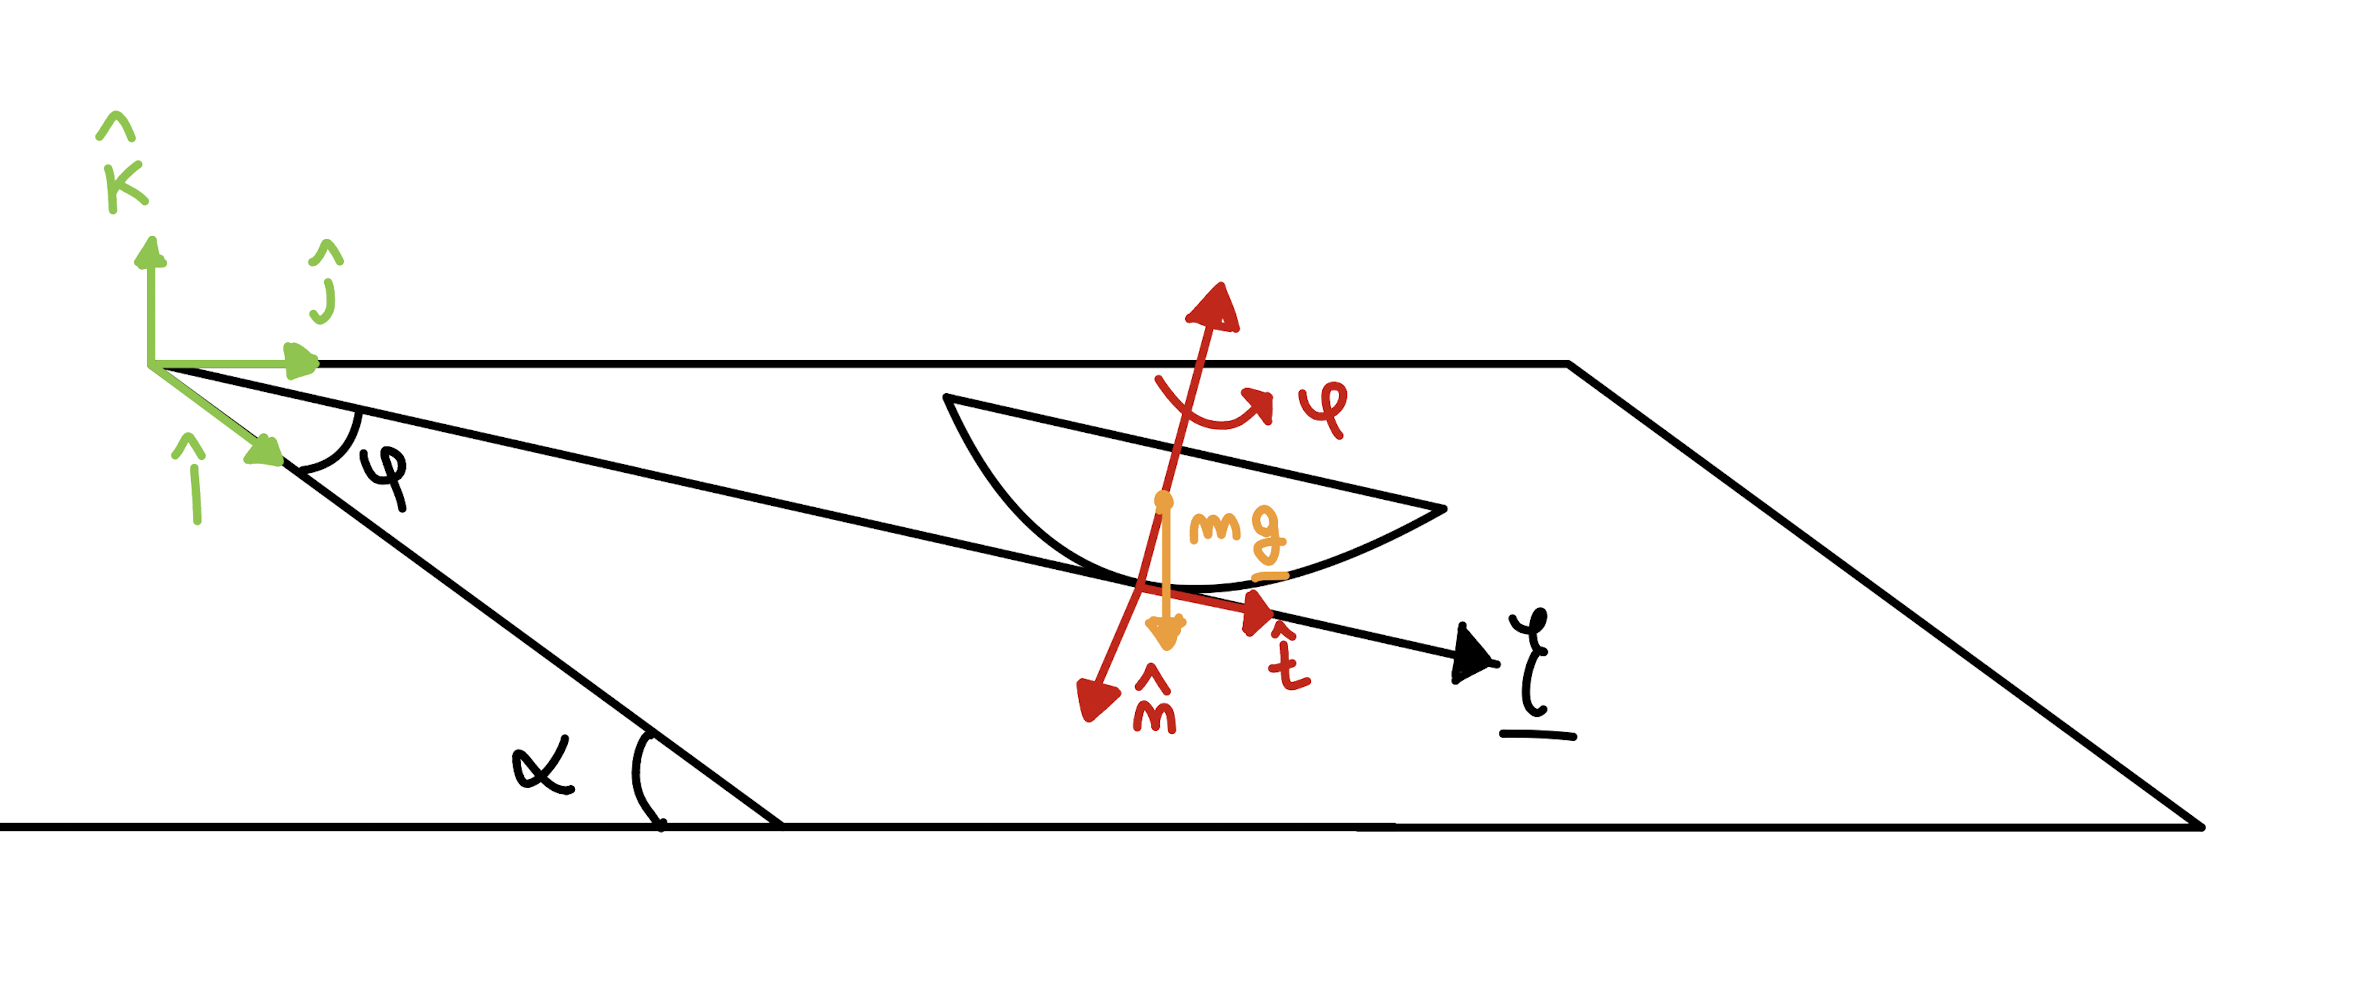
\includegraphics[scale=0.3]{immagini/pattino.png}
  \end{center}
Il pattino può solo avere componente della velocità lungo la propria direzione
(non può derapare). Il pattino sta nel piano verticale \((\hat{\xi},\hat{k})\)

\[
\hat{t}=
\begin{pmatrix}
\cos\varphi\\
\sin\varphi
\end{pmatrix}
\qquad
\hat{n}=
\begin{pmatrix}
+\sin\varphi\\
-\cos\varphi
\end{pmatrix}
\]

Posso scrivere il vincolo
\[
\dot{\underline{x}}_G\cdot \hat{n}=0
\Longleftrightarrow
\dot{x}_G\sin\varphi-\dot{y}_G\cos\varphi=0
\]

Il vincolo è anolonomo. Uso le coordinate libere
\((x_G,y_G,\varphi)\) dipendenti.

\[
T=
\frac{m\dot{x}_G^2}{2}
+
\frac{m\dot{y}_G^2}{2}
+
I\frac{\dot{\varphi}^2}{2}
\qquad
V=-mg\sin\alpha\, x_G
\]

\[
\mathcal{L}=T-V=
\frac{m\dot{x}_G^2}{2}
+
\frac{m\dot{y}_G^2}{2}
+
I\frac{\dot{\varphi}^2}{2}
+
mg\sin\alpha\, x_G
\]

Il vincolo può essere scritto nella forma

\[
\underbrace{
\begin{pmatrix}
-\sin\varphi\\
\cos\varphi\\
0
\end{pmatrix}
}_{\underline{a}}
\cdot
\begin{pmatrix}
\dot{x}_G\\
\dot{y}_G\\
\dot{\varphi}
\end{pmatrix}
=0
\]

Scrivo

\[
\frac{d}{dt}
\left(
\frac{\partial \mathcal{L}}{\partial \dot{q}_j}
\right)
-
\frac{\partial \mathcal{L}}{\partial q_j}
=
a_j\lambda
\qquad
\forall j
\]

ovvero

\[
\begin{cases}
m\ddot{x}_G-mg\sin\alpha=-\lambda\sin\varphi\\
m\ddot{y}_G=\lambda\cos\varphi\\
I\ddot{\varphi}=0\\
-\dot{x}_G\sin\varphi+\dot{y}_G\cos\varphi=0
\end{cases}
\]

Suppongo
\[
\varphi(0)=0
\qquad
\dot{\varphi}(0)=\omega
\Rightarrow
\varphi(t)=\omega t
\]

Utilizziamo l'integrale primo dell'energia dove
\[
x_G(0)=y_G(0)=0
\]
\[
\dot{x}_G(0)=\dot{y}_G(0)=0
\]

\[
\frac{m\dot{x}_G^2}{2}
+
\frac{m\dot{y}_G^2}{2}
+
I\frac{\omega^2}{2}
-
mgx_G\sin\alpha
=
I\frac{\omega^2}{2}
\]

\[
\begin{cases}
\frac{m}{2}\dot{x}_G^2
+
\frac{m}{2}\dot{y}_G^2
-
mg\sin\alpha\,x_G=0\\
\dot{x}_G\sin\varphi-\dot{y}_G\cos\varphi=0
\end{cases}
\Rightarrow
\begin{cases}
\frac{m}{2}\dot{x}_G^2
+
\frac{m}{2}\dot{x}_G^2\tg^2\varphi
-
mg\sin\alpha\,x_G=0\\
\dot{y}_G=\dot{x}_G\tg\varphi
\end{cases}
\]

\[
\frac{m}{2}\dot{x}_G^2
\left(
1+\tg^2\varphi
\right)
=
mg\sin\alpha\,x_G
\Rightarrow
\dot{x}_G^2
=
2g\sin\alpha\,x_G\cdot \cos^2\varphi
\]

\[
\Rightarrow
\dot{x}_G
=
\sqrt{2g\sin\alpha}\cos\varphi\sqrt{x_G}
\]

\[
\Rightarrow
\frac{\dot{x}_G}{\sqrt{x_G}}
=
\sqrt{2g\sin\alpha}\cos(\omega t)
\Rightarrow
\int
\frac{1}{\sqrt{x_G}}\,dx_G
=
\int
\sqrt{2g\sin\alpha}\cos(\omega t)\,dt
\]

\[
\Rightarrow
2\sqrt{x_G}
=
\sqrt{2g\sin\alpha}\frac{\sin(\omega t)}{\omega}
+
C
\]

Impongo
\[
x_G(0)=0
\]

\[
\Rightarrow
\sqrt{x_G}
=
\sqrt{\frac{g\sin\alpha}{2}}
\cdot
\frac{\sin(\omega t)}{\omega}
\Rightarrow
x_G
=
\frac{g\sin\alpha}{2}
\frac{\sin^2(\omega t)}{\omega^2}
\]

\[
\Rightarrow
\dot{x}_G
=
g\sin\alpha
\frac{\sin(\omega t)\cos(\omega t)}{\omega}
=
g\sin\alpha
\frac{\sin(2\omega t)}{2\omega}
\]

\[
\dot{y}_G
=
\tg\varphi\,\dot{x}_G
=
g\sin\alpha
\frac{\sin(2\omega t)}{2\omega}
\cdot
\tg(\omega t)
=
g\sin\alpha
\frac{\sin^2(\omega t)}{\omega}
=
\frac{g\sin\alpha}{\omega}
\cdot
\frac{1-\cos(2\omega t)}{2}
\]

Integrando \(y_G\) si ottiene

\[
\begin{cases}
x_G(t)
=
\frac{g\sin\alpha}{2\omega^2}
\frac{1-\cos(2\omega t)}{2}\\
y_G(t)
=
\frac{g\sin\alpha}{2\omega}
\left(
t-\frac{\sin(2\omega t)}{2\omega}
\right)
\end{cases}
\]
\begin{center}
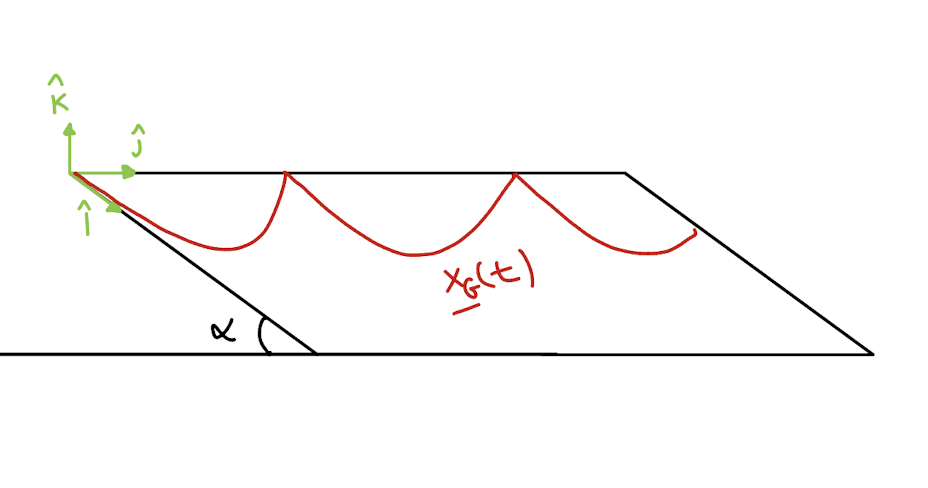
\includegraphics[scale=0.6]{immagini/pattino_1.png}
\end{center}

\end{example}

\chapter{Il pendolo di Kapitza}

In questa lezione studieremo un sistema meccanico derivato dal pendolo semplice detto pendolo di Kapitza. Il pendolo in questione è un pendolo semplice con cerniera superiore mobile e fatta oscillare ad una frequenza elevata con piccole oscillazioni. Sia $y_0(t)$ la posizione della cerniera.

\begin{center}
\begin{tikzpicture}[scale=1.2,>=Latex]
    \coordinate (O) at (0,0);
    \coordinate (M) at (1.8,-2.4);

    \draw[fill=white,line width=0.8pt] (O) circle (0.14);
    \node[left=4pt] at (O) {$O$};

    \draw[->,line width=0.9pt] (0,0.55) -- (0,0.15);
    \draw[->,line width=0.9pt] (0,-0.15) -- (0,-0.55);

    \draw[line width=0.9pt] (O) -- (M);
    \node[right] at (0.8,-1.0) {$\ell$};

    \fill (M) circle (0.14);
\end{tikzpicture}
\end{center}

Per modellizzare le piccole oscillazioni ad alta frequenza usiamo
\[
y_0(t)=a\cos(\omega t)
\qquad
a\ll \ell
\qquad
\omega \gg \sqrt{\frac{g}{\ell}}=\omega_0
\]

Dove $\ell$ e $\omega_0$ sono lunghezza e pulsazione del pendolo semplice.

Per scrivere le equazioni del moto di questo pendolo ci mettiamo nel sistema di riferimento (non inerziale) della cerniera. Devo aggiungere nel bilancio delle forze la forza apparente dovuta al moto della cerniera.

\[
y_0(t)=a\cos(\omega t)
\qquad \Rightarrow \qquad
\dot{y}_0(t)=-a\omega\sin(\omega t)
\qquad \Rightarrow \qquad
\ddot{y}_0(t)=-a\omega^2\cos(\omega t)
\]

Notiamo che nel nuovo sistema di riferimento non inerziale il polo appare di nuovo incernierato

\begin{center}
\begin{tikzpicture}[scale=1.25,>=Latex]
    \definecolor{mygreen}{RGB}{130,180,60}
    \definecolor{myred}{RGB}{210,40,30}

    % assi
    \draw[mygreen,->,line width=0.9pt] (-1.6,0.8) -- (-0.55,0.8);
    \node[mygreen,above] at (-1.0,0.8) {$\hat{\imath}$};

    \draw[mygreen,->,line width=0.9pt] (-1.6,0.8) -- (-1.6,1.8);
    \node[mygreen,left] at (-1.6,1.4) {$\hat{k}$};

    \draw[mygreen,line width=0.8pt] (-2.0,0.45) circle (0.18);
    \draw[mygreen,line width=0.8pt] (-2.1,0.35) -- (-1.9,0.55);
    \draw[mygreen,line width=0.8pt] (-2.1,0.55) -- (-1.9,0.35);
    \node[mygreen,left] at (-2.1,0.45) {$\hat{\jmath}$};

    % pendolo
    \coordinate (P) at (0,1.2);
    \coordinate (V) at (0,-0.2);
    \coordinate (M) at ($(P)+(-65:1.55)$);

    \draw[dashed,line width=0.8pt] (P) -- (V);
    \draw[line width=0.9pt] (P) -- (M);

    \draw[line width=0.8pt] (P) circle (0.12);
    \draw[line width=0.8pt] ($(P)+(-0.08,-0.08)$) -- ($(P)+(0.08,0.08)$);
    \draw[line width=0.8pt] ($(P)+(-0.08,0.08)$) -- ($(P)+(0.08,-0.08)$);

    \fill (M) circle (0.14);

    % angolo theta senza libreria angles
    \draw[->,line width=0.8pt]
        ($(P)+(0,-0.45)$) arc[start angle=-90,end angle=-65,radius=0.45];

    \node at ($(P)+(-77:0.65)$) {$\theta$};

    % forze
    \draw[myred,->,line width=0.9pt] (M) -- ++(0,1.05);
    \node[myred,right] at ($(M)+(0,0.55)$) {$ma\omega^2\cos(\omega t)$};

    \draw[mygreen,->,line width=0.9pt] (M) -- ++(0,-1.0);
    \node[mygreen,right] at ($(M)+(0,-0.55)$) {$mg$};
\end{tikzpicture}
\end{center}

Scrivo la seconda equazione cardinale
\[
\frac{d}{dt}\left(\underline{\ell}\wedge m\ell\dot{\theta}\,\hat{t}\right)
=
\underline{\ell}\wedge -mg\hat{k}
+
\underline{\ell}\wedge ma\omega^2\cos(\omega t)\hat{k}
\]

\[
\frac{d}{dt}\left(-\ell^2m\dot{\theta}\right)
=
+mg\ell\sin\theta
-\ell ma\omega^2\cos(\omega t)\sin\theta
\Longleftrightarrow
\ddot{\theta}
=
-\frac{g}{\ell}\sin\theta
+
\frac{m\ell a\omega^2}{m\ell^2}\cos(\omega t)\sin\theta
\]

\[
\Longleftrightarrow
\ddot{\theta}
=
-\omega_0^2\sin\theta
+
\frac{a}{\ell}\omega^2\cos(\omega t)\sin\theta
\Longleftrightarrow
\ddot{\theta}
=
-\omega_0^2\sin\theta
\left(
1-\frac{a}{\ell}\frac{\omega^2}{\omega_0^2}\cos(\omega t)
\right)
\]

Adimensionalizziamo il tempo. Poniamo
\[
t'=\omega_0 t
\Longleftrightarrow
t=\frac{t'}{\omega_0}.
\]
Ricordiamo che
\[
\frac{d}{dt}f(t)
=
\frac{d}{dt}f(t'(t))
=
\frac{d}{dt'}f(t')\cdot \frac{dt'}{dt}
=
\frac{d}{dt'}f(t')\cdot \omega_0
\]

Allora
\[
\omega_0^2\frac{d^2}{dt'^2}\theta
=
-\omega_0^2\sin\theta
\left(
1-\frac{a}{\ell}\frac{\omega^2}{\omega_0^2}
\cos\left(\frac{\omega}{\omega_0}t'\right)
\right)
\]

\[
\Longleftrightarrow
\frac{d^2}{dt'^2}\theta
=
-\sin\theta
\left(
1-\frac{a}{\ell}\cdot \frac{\omega^2}{\omega_0^2}
\cos\left(\frac{\omega}{\omega_0}t'\right)
\right)
\]

Impongo che
\[
\frac{\omega_0}{\omega}=\varepsilon
\qquad \text{e definisco} \qquad
b = \frac{a}{\ell}\frac{\omega}{\omega_0} = \frac{a}{\ell}\frac{1}{\varepsilon} \sim 1
\]
e ribattezzo $t'=t$.

\[
\ddot{\theta}
=
-\sin\theta
\left(
1-\frac{b}{\varepsilon}\cos\left(\frac{t}{\varepsilon}\right)
\right)
\]

Il nostro sistema si muove su 2 periodi diversi: uno breve delle piccole oscillazioni e uno lungo del pendolo semplice.

Vorremmo separare ciò che succede nei tempi lunghi $(\sim 1)$ da ciò che succede su tempi corti $\left(\sim \frac{1}{\varepsilon}\right)$ e poi mediare sul periodo breve.

Per capire a livello intuitivo quello che facciamo possiamo pensare ad una ruota che gira ad altissima frequenza, migliaia di giri al secondo, e ad una videocamera che registra a $30$ fps. La videocamera si accorge del moto solo ogni $1/30$ secondi e quindi ad una giusta frequenza dei giri della ruota questa potrebbe addirittura apparire ferma.

Rappresentiamo $\theta(t)$ come una funzione di 2 variabili $\tilde{\theta}(t,\tau)$ dove $t$ è il tempo lento e
\[
\tau:=\frac{t}{\varepsilon}
\]
è il tempo veloce
\[
\theta(t)=\tilde{\theta}(t,\tau)
\]

Vogliamo tener conto alla scala lenta dell'influenza delle oscillazioni della cerniera ad alta frequenza

\[
\frac{d\theta}{dt}
=
\frac{\partial \tilde{\theta}}{\partial t}
+
\frac{\partial \tilde{\theta}}{\partial \tau}\cdot \frac{\partial \tau}{\partial t}
=
\frac{\partial \tilde{\theta}}{\partial t}
+
\frac{1}{\varepsilon}\frac{\partial \tilde{\theta}}{\partial \tau}
\]

D'ora in poi $\tilde{\theta}=\theta$ e risolviamo l'equazione

\[
\left(
\frac{\partial}{\partial t}
+
\frac{1}{\varepsilon}\frac{\partial}{\partial \tau}
\right)
\left(
\frac{\partial}{\partial t}
+
\frac{1}{\varepsilon}\frac{\partial}{\partial \tau}
\right)
\theta
=
-\sin\theta
\left(
1-\frac{b}{\varepsilon}\cos(\tau)
\right)
\]

Siamo passati ad un'equazione differenziale alle derivate parziali

\[
\frac{\partial^2\theta}{\partial t^2}
+
\frac{2}{\varepsilon}
\frac{\partial^2\theta}{\partial \tau \partial t}
+
\frac{1}{\varepsilon^2}
\frac{\partial^2\theta}{\partial \tau^2}
=
-\sin\theta
\left(
1-\frac{b}{\varepsilon}\cos\tau
\right)
\]

Supponiamo che $\theta$ dipenda in modo liscio da $\varepsilon$ e che per $\varepsilon$ piccolo converga

\[
\theta(t,\tau;\varepsilon)
=
\theta_0(t,\tau)
+
\varepsilon \theta_1(t,\tau)
+
\ldots
\]

Inserisco nell'equazione

\[
\frac{\partial^2}{\partial t^2}(\theta_0+\varepsilon\theta_1)
+
\frac{2}{\varepsilon}
\frac{\partial^2}{\partial t\partial\tau}
(\theta_0+\varepsilon\theta_1)
+
\frac{1}{\varepsilon^2}
\frac{\partial^2}{\partial \tau^2}
(\theta_0+\varepsilon\theta_1)
=
-\sin(\theta_0+\varepsilon\theta_1)
\left(
1-\frac{b}{\varepsilon}\cos\tau
\right)
=
\]

\[
=
-
\left[
\sin\theta_0 \cos(\varepsilon\theta_1)
+
\cos\theta_0 \sin(\varepsilon\theta_1)
\right]
\left(
1-\frac{b}{\varepsilon}\cos\tau
\right)
=
\]

Ricordiamo che
\[
\cos(\varepsilon\theta_1)\sim 1-\frac{\varepsilon^2\theta_1^2}{2},
\qquad
\sin(\varepsilon\theta_1)\sim \varepsilon\theta_1.
\]
Stiamo ignorando tutti gli infinitesimi in $\varepsilon$ di ordine superiore al primo nell'equazione finale (e quindi trascuriamo il termine di ordine 2 del coseno), quindi

\[
\frac{\partial^2}{\partial t^2}(\theta_0+\varepsilon\theta_1)
+
\frac{2}{\varepsilon}
\frac{\partial^2}{\partial t\partial\tau}
(\theta_0+\varepsilon\theta_1)
+
\frac{1}{\varepsilon^2}
\frac{\partial^2}{\partial \tau^2}
(\theta_0+\varepsilon\theta_1)
=
\]

\[
=
-
\left[
\sin\theta_0
+
\cos\theta_0\,\varepsilon\theta_1
\right]
\left(
1-\frac{b}{\varepsilon}\cos\tau
\right)
\]

Questo sviluppo deve valere $\forall \varepsilon$, quindi devo sommare a zero i termini che moltiplicano le stesse potenze di $\varepsilon$. Moltiplico tutto per $\varepsilon^2$ (principio di identità dei polinomi):

\[
\varepsilon^2
\frac{\partial^2}{\partial t^2}(\theta_0+\varepsilon\theta_1)
+
2\varepsilon
\frac{\partial^2}{\partial t\partial\tau}
(\theta_0+\varepsilon\theta_1)
+
\frac{\partial^2}{\partial \tau^2}
(\theta_0+\varepsilon\theta_1)
=
-
\left[
\sin\theta_0
+
\varepsilon\theta_1\cos\theta_0
\right]
(\varepsilon^2-\varepsilon b\cos\tau)
\]

Uguaglio i termini di ordine $\varepsilon^0=1$

\[
\frac{\partial^2}{\partial \tau^2}\theta_0=0
\qquad \Rightarrow \qquad
\theta_0=A(t)\tau+B(t)
\]

Devo porre $A(t)=0$ perché voglio che $\theta_0$ sia periodica. Ottengo quindi $\theta_0(t)$ sola funzione di $t$.

Faccio lo stesso con i termini di ordine $\varepsilon^1$. Notiamo che

\[
\frac{\partial^2}{\partial t\partial\tau}\theta_0(t)
=
\frac{\partial}{\partial \tau}
\left(
\frac{d}{dt}\theta_0(t)
\right)
=
0
\]

Allora
\[
\frac{\partial^2 \theta_1}{\partial \tau^2}
=
b\sin\theta_0\cos\tau
\qquad \Rightarrow \qquad
\theta_1
=
-b\sin\theta_0\cos\tau
+
A(t)\tau
+
B(t)
\]

Per lo stesso motivo di prima pongo $A(t)=0$ e $B(t)$ lo pongo convenzionalmente uguale a $0$.
Dobbiamo cercare soluzioni del tipo

\[
\theta(t,\tau)
=
\theta_0
+
\varepsilon\theta_1
=
\theta_0(t)
-
\varepsilon b\sin\theta_0\cos(\tau)
\]

Adesso che dinamica lenta e veloce sono disaccoppiate possiamo fare una media delle equazioni del moto sul periodo veloce e tenere solo la dinamica lenta.

Riprendiamo le equazioni in forma adimensionata

\[
\frac{d^2\theta}{dt^2}
=
-\sin\theta
\left(
1-\frac{a}{\ell}
\left(
\frac{\omega}{\omega_0}
\right)^2
\cos(\tau)
\right)
\]

e inseriamo $\theta(t,\tau)$

\[
\frac{d^2}{dt^2}
\left(
\theta_0
-
\varepsilon b\sin\theta_0\cos(\tau)
\right)
=
-\sin
\left(
\theta_0
-
\varepsilon b\sin\theta_0\cos\tau
\right)
\left(
1-\frac{b}{\varepsilon}
\cos(\tau)
\right)
\]

Integro tra $0$ e $2\pi$ in $d\tau$ (la media sul periodo veloce corrisponde poi a dividere per $2\pi$)

\[
\int_0^{2\pi}
\frac{d^2\theta_0}{dt^2}
\,d\tau
=
\frac{d^2\theta_0}{dt^2}\cdot 2\pi
\]

\[
\int_0^{2\pi}
-
\frac{d^2}{dt^2}
\varepsilon b\sin\theta_0\cos\tau
\,d\tau
=
0
\]

Elaboro i termini a destra

\[
-
\left[
\sin\theta_0
\overbrace{
\cos(\varepsilon b\sin\theta_0\cos\tau)
}^{\sim 1}
-
\cos\theta_0
\overbrace{
\sin(\varepsilon b\sin\theta_0\cos\tau)
}^{\sim \varepsilon b\sin\theta_0\cos\tau}
\right]
\left(
1-\frac{b}{\varepsilon}
\cos\tau
\right)
=
\]

\[
=
-
\left[
\sin\theta_0
-
\cos\theta_0\,\varepsilon b\sin\theta_0\cos\tau
\right]
\left(
1-\frac{b}{\varepsilon}
\cos\tau
\right)
\]

\[
\int_0^{2\pi}
-\sin\theta_0\,d\tau
=
-2\pi\sin\theta_0
\]

I due termini lineari in $\cos\tau$ hanno media nulla su un periodo. Rimane il termine quadratico:

\[
-
\int_0^{2\pi}
\left(\varepsilon b\cos\theta_0\sin\theta_0\right)
\left(\frac{b}{\varepsilon}\right)
\cos^2(\tau)
\,d\tau
=
-
b^2
\cos\theta_0\sin\theta_0
\int_0^{2\pi}
\frac{1+\cos(2\tau)}{2}
\,d\tau
=
-
b^2
\cos\theta_0\sin\theta_0\,\pi
\]

Sommando i termini e dividendo per $2\pi$, otteniamo l'equazione mediata nel tempo adimensionale $t'$ (che avevamo ribattezzato $t$):

\[
\frac{d^2\theta_0}{dt'^2}
=
-\sin\theta_0
-
\frac{b^2}{2}\sin\theta_0\cos\theta_0
\]

Ritorniamo ora al tempo fisico $t_{phys}$. Scrivendo esplicitamente la catena delle derivate $\frac{d}{dt_{phys}} = \omega_0 \frac{d}{dt'}$, si ha $\frac{d^2}{dt_{phys}^2} = \omega_0^2 \frac{d^2}{dt'^2}$. Moltiplichiamo quindi l'equazione adimensionale per $\omega_0^2$:

\[
\ddot{\theta}_0
=
-\omega_0^2\sin\theta_0
\left(
1+
\frac{b^2}{2}\cos\theta_0
\right)
\]

In questa equazione il tempo veloce è scomparso ma se ne tiene conto in modo mediato (efficace) nel termine tra parentesi. Rinominando $\theta=\theta_0$:

\[
\ddot{\theta}
=
-\omega_0^2\sin\theta
\left(
1+\frac{b^2}{2}\cos\theta
\right)
\]

Supponiamo che questa equazione derivi da un potenziale efficace $V_{\text{eff}}$. Affinché il potenziale abbia le unità di misura corrette di un'energia, moltiplichiamo l'equazione per $m\ell^2$:

\[
m\ell^2\ddot{\theta}
=
-\frac{\partial V_{\text{eff}}}{\partial \theta}
\Rightarrow
\frac{\partial V_{\text{eff}}}{\partial \theta}
=
m\ell^2\omega_0^2\sin\theta
\left(
1+\frac{b^2}{2}\cos\theta
\right)
\]

Le configurazioni di equilibrio si trovano annullando la derivata:

\[
\theta_1=0
\qquad
\theta_2=\pi
\qquad
\cos\theta_{3,4}
=
-\frac{2}{b^2}
\qquad
\left(\exists \text{ se } \frac{2}{b^2}<1 \Longleftrightarrow b^2>2 \Longleftrightarrow b>\sqrt{2}\right)
\]

\begin{center}
\begin{tikzpicture}[scale=1.15]
    \coordinate (O) at (0,0);

    \draw[line width=0.9pt] (O) -- (0,-1.6);
    \draw[line width=0.9pt] (O) -- (0,1.6);
    \draw[line width=0.9pt] (O) -- (1.25,1.15);
    \draw[line width=0.9pt] (O) -- (-1.25,1.15);

    \fill (O) circle (0.11);
    \draw[line width=0.8pt] (-0.11,-0.11) -- (0.11,0.11);
    \draw[line width=0.8pt] (-0.11,0.11) -- (0.11,-0.11);

    \fill (0,-1.6) circle (0.08);
    \fill (0,1.6) circle (0.08);
    \fill (1.25,1.15) circle (0.08);
    \fill (-1.25,1.15) circle (0.08);

    \node[right] at (0,-1.6) {$\theta_1$};
    \node[right] at (0,1.6) {$\theta_2$};
    \node[right] at (1.25,1.15) {$\theta_3$};
    \node[left] at (-1.25,1.15) {$\theta_4$};
\end{tikzpicture}
\end{center}

\[
\frac{\partial^2 V_{\text{eff}}}{\partial \theta^2}
=
m\ell^2\omega_0^2\cos\theta
\left(
1+\frac{b^2}{2}\cos\theta
\right)
-
m\ell^2\omega_0^2\sin^2\theta
\left(
\frac{b^2}{2}
\right)
\]

\[
\left.
\frac{d^2 V_{\text{eff}}}{d\theta^2}
\right|_{\theta=0}
=
m\ell^2\omega_0^2
\left(
1+\frac{b^2}{2}
\right)
>
0
\]

Stabile sempre.

\[
\left.
\frac{d^2 V_{\text{eff}}}{d\theta^2}
\right|_{\theta=\pi}
=
-m\ell^2\omega_0^2
\left(
1-\frac{b^2}{2}
\right)
=
m\ell^2\omega_0^2
\left(
\frac{b^2}{2}-1
\right)
>
0
\Longleftrightarrow
b^2>2
\]

Stabile per $b^2>2$ (ovvero $b>\sqrt{2}$), che è esattamente la condizione di esistenza per $\theta_{3,4}$.
\[
\left.
\frac{d^2V_{\text{eff}}}{d\theta^2}
\right|_{\theta_3,\theta_4}
=
m\ell^2\omega_0^2
\left(
-\frac{2}{b^2}
\right)
\left(
1+\frac{b^2}{2}
\left(
-\frac{2}{b^2}
\right)
\right)
-
m\ell^2\omega_0^2
\frac{b^2}{2}
\left(
1-\frac{4}{b^4}
\right)
=
-m\ell^2\omega_0^2
\left(
\frac{b^2}{2}
-
\frac{2}{b^2}
\right)
<0
\]

Instabile per $b^2>2$, ovvero ogni volta che esistono $\theta_{3,4}$.

\begin{center}
\begin{tikzpicture}[scale=1.15,>=Latex]

    % -------------------- caso b^2 < 2 --------------------
    \begin{scope}[xshift=-3.9cm]
        \node at (-1.7,1.35) {$b^2<2$};

        % assi
        \draw[->,line width=0.8pt] (-1.6,0) -- (2.1,0);
        \draw[->,line width=0.8pt] (0,-1.25) -- (0,1.45);

        % origine e pi
        \fill (0,0) circle (0.04);
        \node[above right] at (0,0) {$0$};

        \draw[dashed,line width=0.8pt] (1.75,0) -- (1.75,1.05);
        \node[below] at (1.75,0) {$\pi$};

        % etichetta V
        \node at (1.95,1.05) {$V$};

        % curva del potenziale
        \draw[line width=1pt]
            plot[smooth,tension=0.75] coordinates {
                (-1.55,0.90)
                (-1.25,0.75)
                (-0.85,0.25)
                (-0.45,-0.72)
                (0.10,-0.95)
                (0.70,-0.65)
                (1.15,0.00)
                (1.45,0.55)
                (1.75,0.85)
            };
    \end{scope}

    % -------------------- caso b^2 > 2 --------------------
    \begin{scope}[xshift=3.4cm]
        \node at (2.0,0.25) {$b^2>2$};

        % assi
        \draw[->,line width=0.8pt] (-1.4,0) -- (2.4,0);
        \draw[->,line width=0.8pt] (0,-1.25) -- (0,1.45);

        % origine
        \fill (0,0) circle (0.04);
        \node[below left] at (0,0) {$0$};

        % tacche sull'asse
        \draw[line width=0.8pt] (0.90,0.07) -- (0.90,-0.07);
        \node[below] at (0.90,0) {$\theta_3$};

        \draw[line width=0.8pt] (1.35,0.07) -- (1.35,-0.07);
        \node[below] at (1.35,0) {$\pi$};

        \draw[line width=0.8pt] (1.80,0.07) -- (1.80,-0.07);
        \node[below] at (1.80,0) {$\theta_4$};

        % etichetta V
        \node[red] at (1.75,1.05) {$V$};

        % curva del potenziale
        \draw[red,line width=1pt]
            plot[smooth,tension=0.9] coordinates {
                (-0.65,-1.00)
                (-0.25,-0.95)
                (0.15,-0.70)
                (0.50,0.10)
                (0.85,0.85)
                (1.15,0.70)
                (1.35,0.55)
                (1.60,0.72)
                (1.85,0.90)
                (2.10,0.45)
                (2.20,0.05)
            };
    \end{scope}

\end{tikzpicture}
\end{center}


\end{document}
